% Options for packages loaded elsewhere
% Options for packages loaded elsewhere
\PassOptionsToPackage{unicode}{hyperref}
\PassOptionsToPackage{hyphens}{url}
\PassOptionsToPackage{dvipsnames,svgnames,x11names}{xcolor}
%
\documentclass[
  french,
  11pt,
  a4paper,
]{scrbook}
\usepackage{xcolor}
\usepackage[margin=2.5cm]{geometry}
\usepackage{amsmath,amssymb}
\setcounter{secnumdepth}{5}
\usepackage{iftex}
\ifPDFTeX
  \usepackage[T1]{fontenc}
  \usepackage[utf8]{inputenc}
  \usepackage{textcomp} % provide euro and other symbols
\else % if luatex or xetex
  \usepackage{unicode-math} % this also loads fontspec
  \defaultfontfeatures{Scale=MatchLowercase}
  \defaultfontfeatures[\rmfamily]{Ligatures=TeX,Scale=1}
\fi
\usepackage{lmodern}
\ifPDFTeX\else
  % xetex/luatex font selection
\fi
% Use upquote if available, for straight quotes in verbatim environments
\IfFileExists{upquote.sty}{\usepackage{upquote}}{}
\IfFileExists{microtype.sty}{% use microtype if available
  \usepackage[]{microtype}
  \UseMicrotypeSet[protrusion]{basicmath} % disable protrusion for tt fonts
}{}
\makeatletter
\@ifundefined{KOMAClassName}{% if non-KOMA class
  \IfFileExists{parskip.sty}{%
    \usepackage{parskip}
  }{% else
    \setlength{\parindent}{0pt}
    \setlength{\parskip}{6pt plus 2pt minus 1pt}}
}{% if KOMA class
  \KOMAoptions{parskip=half}}
\makeatother
% Make \paragraph and \subparagraph free-standing
\makeatletter
\ifx\paragraph\undefined\else
  \let\oldparagraph\paragraph
  \renewcommand{\paragraph}{
    \@ifstar
      \xxxParagraphStar
      \xxxParagraphNoStar
  }
  \newcommand{\xxxParagraphStar}[1]{\oldparagraph*{#1}\mbox{}}
  \newcommand{\xxxParagraphNoStar}[1]{\oldparagraph{#1}\mbox{}}
\fi
\ifx\subparagraph\undefined\else
  \let\oldsubparagraph\subparagraph
  \renewcommand{\subparagraph}{
    \@ifstar
      \xxxSubParagraphStar
      \xxxSubParagraphNoStar
  }
  \newcommand{\xxxSubParagraphStar}[1]{\oldsubparagraph*{#1}\mbox{}}
  \newcommand{\xxxSubParagraphNoStar}[1]{\oldsubparagraph{#1}\mbox{}}
\fi
\makeatother

\usepackage{color}
\usepackage{fancyvrb}
\newcommand{\VerbBar}{|}
\newcommand{\VERB}{\Verb[commandchars=\\\{\}]}
\DefineVerbatimEnvironment{Highlighting}{Verbatim}{commandchars=\\\{\}}
% Add ',fontsize=\small' for more characters per line
\newenvironment{Shaded}{}{}
\newcommand{\AlertTok}[1]{\textcolor[rgb]{1.00,0.33,0.33}{\textbf{#1}}}
\newcommand{\AnnotationTok}[1]{\textcolor[rgb]{0.42,0.45,0.49}{#1}}
\newcommand{\AttributeTok}[1]{\textcolor[rgb]{0.84,0.23,0.29}{#1}}
\newcommand{\BaseNTok}[1]{\textcolor[rgb]{0.00,0.36,0.77}{#1}}
\newcommand{\BuiltInTok}[1]{\textcolor[rgb]{0.84,0.23,0.29}{#1}}
\newcommand{\CharTok}[1]{\textcolor[rgb]{0.01,0.18,0.38}{#1}}
\newcommand{\CommentTok}[1]{\textcolor[rgb]{0.42,0.45,0.49}{#1}}
\newcommand{\CommentVarTok}[1]{\textcolor[rgb]{0.42,0.45,0.49}{#1}}
\newcommand{\ConstantTok}[1]{\textcolor[rgb]{0.00,0.36,0.77}{#1}}
\newcommand{\ControlFlowTok}[1]{\textcolor[rgb]{0.84,0.23,0.29}{#1}}
\newcommand{\DataTypeTok}[1]{\textcolor[rgb]{0.84,0.23,0.29}{#1}}
\newcommand{\DecValTok}[1]{\textcolor[rgb]{0.00,0.36,0.77}{#1}}
\newcommand{\DocumentationTok}[1]{\textcolor[rgb]{0.42,0.45,0.49}{#1}}
\newcommand{\ErrorTok}[1]{\textcolor[rgb]{1.00,0.33,0.33}{\underline{#1}}}
\newcommand{\ExtensionTok}[1]{\textcolor[rgb]{0.84,0.23,0.29}{\textbf{#1}}}
\newcommand{\FloatTok}[1]{\textcolor[rgb]{0.00,0.36,0.77}{#1}}
\newcommand{\FunctionTok}[1]{\textcolor[rgb]{0.44,0.26,0.76}{#1}}
\newcommand{\ImportTok}[1]{\textcolor[rgb]{0.01,0.18,0.38}{#1}}
\newcommand{\InformationTok}[1]{\textcolor[rgb]{0.42,0.45,0.49}{#1}}
\newcommand{\KeywordTok}[1]{\textcolor[rgb]{0.84,0.23,0.29}{#1}}
\newcommand{\NormalTok}[1]{\textcolor[rgb]{0.14,0.16,0.18}{#1}}
\newcommand{\OperatorTok}[1]{\textcolor[rgb]{0.14,0.16,0.18}{#1}}
\newcommand{\OtherTok}[1]{\textcolor[rgb]{0.44,0.26,0.76}{#1}}
\newcommand{\PreprocessorTok}[1]{\textcolor[rgb]{0.84,0.23,0.29}{#1}}
\newcommand{\RegionMarkerTok}[1]{\textcolor[rgb]{0.42,0.45,0.49}{#1}}
\newcommand{\SpecialCharTok}[1]{\textcolor[rgb]{0.00,0.36,0.77}{#1}}
\newcommand{\SpecialStringTok}[1]{\textcolor[rgb]{0.01,0.18,0.38}{#1}}
\newcommand{\StringTok}[1]{\textcolor[rgb]{0.01,0.18,0.38}{#1}}
\newcommand{\VariableTok}[1]{\textcolor[rgb]{0.89,0.38,0.04}{#1}}
\newcommand{\VerbatimStringTok}[1]{\textcolor[rgb]{0.01,0.18,0.38}{#1}}
\newcommand{\WarningTok}[1]{\textcolor[rgb]{1.00,0.33,0.33}{#1}}

\usepackage{longtable,booktabs,array}
\newcounter{none} % for unnumbered tables
\usepackage{calc} % for calculating minipage widths
% Correct order of tables after \paragraph or \subparagraph
\usepackage{etoolbox}
\makeatletter
\patchcmd\longtable{\par}{\if@noskipsec\mbox{}\fi\par}{}{}
\makeatother
% Allow footnotes in longtable head/foot
\IfFileExists{footnotehyper.sty}{\usepackage{footnotehyper}}{\usepackage{footnote}}
\makesavenoteenv{longtable}
\usepackage{graphicx}
\makeatletter
\newsavebox\pandoc@box
\newcommand*\pandocbounded[1]{% scales image to fit in text height/width
  \sbox\pandoc@box{#1}%
  \Gscale@div\@tempa{\textheight}{\dimexpr\ht\pandoc@box+\dp\pandoc@box\relax}%
  \Gscale@div\@tempb{\linewidth}{\wd\pandoc@box}%
  \ifdim\@tempb\p@<\@tempa\p@\let\@tempa\@tempb\fi% select the smaller of both
  \ifdim\@tempa\p@<\p@\scalebox{\@tempa}{\usebox\pandoc@box}%
  \else\usebox{\pandoc@box}%
  \fi%
}
% Set default figure placement to htbp
\def\fps@figure{htbp}
\makeatother



\ifLuaTeX
\usepackage[bidi=basic,shorthands=off]{babel}
\else
\usepackage[bidi=default,shorthands=off]{babel}
\fi
\ifLuaTeX
  \usepackage{selnolig} % disable illegal ligatures
\fi


\setlength{\emergencystretch}{3em} % prevent overfull lines

\providecommand{\tightlist}{%
  \setlength{\itemsep}{0pt}\setlength{\parskip}{0pt}}



 


\makeatletter
\@ifpackageloaded{tcolorbox}{}{\usepackage[skins,breakable]{tcolorbox}}
\@ifpackageloaded{fontawesome5}{}{\usepackage{fontawesome5}}
\definecolor{quarto-callout-color}{HTML}{909090}
\definecolor{quarto-callout-note-color}{HTML}{0758E5}
\definecolor{quarto-callout-important-color}{HTML}{CC1914}
\definecolor{quarto-callout-warning-color}{HTML}{EB9113}
\definecolor{quarto-callout-tip-color}{HTML}{00A047}
\definecolor{quarto-callout-caution-color}{HTML}{FC5300}
\definecolor{quarto-callout-color-frame}{HTML}{acacac}
\definecolor{quarto-callout-note-color-frame}{HTML}{4582ec}
\definecolor{quarto-callout-important-color-frame}{HTML}{d9534f}
\definecolor{quarto-callout-warning-color-frame}{HTML}{f0ad4e}
\definecolor{quarto-callout-tip-color-frame}{HTML}{02b875}
\definecolor{quarto-callout-caution-color-frame}{HTML}{fd7e14}
\makeatother
\makeatletter
\@ifpackageloaded{bookmark}{}{\usepackage{bookmark}}
\makeatother
\makeatletter
\@ifpackageloaded{caption}{}{\usepackage{caption}}
\AtBeginDocument{%
\ifdefined\contentsname
  \renewcommand*\contentsname{Table des matières}
\else
  \newcommand\contentsname{Table des matières}
\fi
\ifdefined\listfigurename
  \renewcommand*\listfigurename{Liste des Figures}
\else
  \newcommand\listfigurename{Liste des Figures}
\fi
\ifdefined\listtablename
  \renewcommand*\listtablename{Liste des Tables}
\else
  \newcommand\listtablename{Liste des Tables}
\fi
\ifdefined\figurename
  \renewcommand*\figurename{Figure}
\else
  \newcommand\figurename{Figure}
\fi
\ifdefined\tablename
  \renewcommand*\tablename{Table}
\else
  \newcommand\tablename{Table}
\fi
}
\@ifpackageloaded{float}{}{\usepackage{float}}
\floatstyle{ruled}
\@ifundefined{c@chapter}{\newfloat{codelisting}{h}{lop}}{\newfloat{codelisting}{h}{lop}[chapter]}
\floatname{codelisting}{Listing}
\newcommand*\listoflistings{\listof{codelisting}{Liste des Listings}}
\makeatother
\makeatletter
\makeatother
\makeatletter
\@ifpackageloaded{caption}{}{\usepackage{caption}}
\@ifpackageloaded{subcaption}{}{\usepackage{subcaption}}
\makeatother
\makeatletter
\@ifpackageloaded{tcolorbox}{}{\usepackage[skins,breakable]{tcolorbox}}
\makeatother
\makeatletter
\@ifundefined{shadecolor}{\definecolor{shadecolor}{HTML}{2E5A88}}{}
\makeatother
\makeatletter
\makeatother
\makeatletter
\ifdefined\Shaded\renewenvironment{Shaded}{\begin{tcolorbox}[borderline west={3pt}{0pt}{shadecolor}, boxrule=0pt, breakable, enhanced, frame hidden, interior hidden, sharp corners]}{\end{tcolorbox}}\fi
\makeatother
\usepackage{bookmark}
\IfFileExists{xurl.sty}{\usepackage{xurl}}{} % add URL line breaks if available
\urlstyle{same}
\hypersetup{
  pdftitle={Python pour l'Intelligence Artificielle},
  pdfauthor={Loïc PILET},
  pdflang={fr},
  colorlinks=true,
  linkcolor={Maroon},
  filecolor={Maroon},
  citecolor={Blue},
  urlcolor={Blue},
  pdfcreator={LaTeX via pandoc}}


\title{Python pour l'Intelligence Artificielle}
\usepackage{etoolbox}
\makeatletter
\providecommand{\subtitle}[1]{% add subtitle to \maketitle
  \apptocmd{\@title}{\par {\large #1 \par}}{}{}
}
\makeatother
\subtitle{Spécialisation IA complémentaire à la certification TOSA}
\author{Loïc PILET}
\date{20 avril 2026}
\begin{document}
\frontmatter
\maketitle

\renewcommand*\contentsname{Table des matières}
{
\setcounter{tocdepth}{2}
\tableofcontents
}

\mainmatter
\bookmarksetup{startatroot}

\chapter{Bienvenue}\label{bienvenue}

\bookmarksetup{startatroot}

\chapter*{🐍 Python pour l'Intelligence
Artificielle}\label{python-pour-lintelligence-artificielle}
\addcontentsline{toc}{chapter}{🐍 Python pour l'Intelligence
Artificielle}

\markboth{🐍 Python pour l'Intelligence Artificielle}{🐍 Python pour
l'Intelligence Artificielle}

\section{Un parcours de spécialisation IA complet, en complément de la
certification
TOSA}\label{un-parcours-de-spuxe9cialisation-ia-complet-en-compluxe9ment-de-la-certification-tosa}

Bienvenue dans ce parcours de formation construit sur-mesure pour celles
et ceux qui maîtrisent déjà Python (typiquement via le TOSA) et veulent
se spécialiser en intelligence artificielle.

\begin{tcolorbox}[enhanced jigsaw, arc=.35mm, bottomrule=.15mm, bottomtitle=1mm, breakable, colback=white, colbacktitle=quarto-callout-tip-color!10!white, colframe=quarto-callout-tip-color-frame, coltitle=black, left=2mm, leftrule=.75mm, opacityback=0, opacitybacktitle=0.6, rightrule=.15mm, title=\textcolor{quarto-callout-tip-color}{\faLightbulb}\hspace{0.5em}{Prérequis}, titlerule=0mm, toprule=.15mm, toptitle=1mm]

Tu dois maîtriser les bases Python : variables, boucles, fonctions,
listes, dictionnaires, POO, gestion d'erreurs. Si c'est le cas, tu es
prêt·e à démarrer !

\end{tcolorbox}

\section{🗺️ Le parcours en 3 axes}\label{le-parcours-en-3-axes}

\subsection{🔵 Axe 1 --- Fondations}\label{axe-1-fondations}

\textbf{Modules 1 à 3}

Remise à niveau mathématique, manipulation de données, statistiques
descriptives.

\begin{itemize}
\tightlist
\item
  Module 1 : Maths pour l'IA
\item
  Module 2 : NumPy, Pandas, Matplotlib
\item
  Module 3 : Analyse exploratoire
\end{itemize}

\subsection{🟡 Axe 2 --- Modélisation}\label{axe-2-moduxe9lisation}

\textbf{Modules 4 à 6}

Machine Learning classique puis Deep Learning avec PyTorch.

\begin{itemize}
\tightlist
\item
  Module 4 : ML supervisé
\item
  Module 5 : ML non supervisé
\item
  Module 6 : Deep Learning
\end{itemize}

\subsection{🟢 Axe 3 ---
Industrialisation}\label{axe-3-industrialisation}

\textbf{Modules 7 à 8}

IA générative moderne et déploiement en production.

\begin{itemize}
\tightlist
\item
  Module 7 : LLM, RAG, agents
\item
  Module 8 : MLOps
\end{itemize}

\section{📊 En chiffres}\label{en-chiffres}

{\def\LTcaptype{none} % do not increment counter
\begin{longtable}[]{@{}ll@{}}
\toprule\noalign{}
\endhead
\bottomrule\noalign{}
\endlastfoot
\textbf{Durée totale} & \textasciitilde190 heures \\
\textbf{Nombre de modules} & 8 \\
\textbf{Philosophie pédagogique} & 30\% théorie / 70\% pratique \\
\textbf{Format} & Notebooks + site web + PDF \\
\textbf{Niveau final visé} & AI Engineer junior \\
\end{longtable}
}

\section{🎯 Comment utiliser ce cours}\label{comment-utiliser-ce-cours}

Chaque module est découpé en \textbf{notions} indépendantes mais
progressives. Chaque notion suit la même structure :

\begin{enumerate}
\def\labelenumi{\arabic{enumi}.}
\tightlist
\item
  \textbf{Objectifs pédagogiques} --- ce que tu sauras faire à la fin
\item
  \textbf{Intuition visuelle} --- avant la théorie, on visualise
\item
  \textbf{Théorie appliquée} --- on comprend avant d'apprendre à faire
\item
  \textbf{Code progressif} --- Python pur d'abord, NumPy/bibliothèques
  ensuite
\item
  \textbf{Exercices ciblés} --- un par concept, avec cellules à
  compléter
\item
  \textbf{TP sommatif} --- en fin de module, un projet qui regroupe tout
\end{enumerate}

\begin{tcolorbox}[enhanced jigsaw, arc=.35mm, bottomrule=.15mm, bottomtitle=1mm, breakable, colback=white, colbacktitle=quarto-callout-note-color!10!white, colframe=quarto-callout-note-color-frame, coltitle=black, left=2mm, leftrule=.75mm, opacityback=0, opacitybacktitle=0.6, rightrule=.15mm, title=\textcolor{quarto-callout-note-color}{\faInfo}\hspace{0.5em}{Pour les formateurs}, titlerule=0mm, toprule=.15mm, toptitle=1mm]

Deux versions de chaque notion sont disponibles : une \textbf{version
élève} avec exercices à compléter, et une \textbf{version formateur}
avec corrigés et notes pédagogiques.

\end{tcolorbox}

\section{🚀 Par où commencer ?}\label{par-ouxf9-commencer}

\href{modules/module_01/index.qmd}{\textbf{→ Aller au Module 1 :
Mathématiques pour l'IA}}

Ou, si tu veux piocher directement : utilise la barre latérale ou la
recherche (icône 🔍 en haut).

\part{Axe 1 --- Fondations}

\chapter{Module 1 --- Mathématiques pour
l'IA}\label{module-1-mathuxe9matiques-pour-lia}

Le strict nécessaire pour comprendre (et pas juste appliquer)

\hfill\break

\section{🎯 Pourquoi ce module ?}\label{pourquoi-ce-module}

La plupart des parcours d'IA supposent que tu as un bagage mathématique
solide (bac+3 en maths, école d'ingé\ldots). Ce n'est pas forcément ton
cas, et c'est OK. Ce module te donne \textbf{exactement ce qu'il faut}
--- ni plus ni moins --- pour comprendre tous les modules suivants.

\begin{tcolorbox}[enhanced jigsaw, arc=.35mm, bottomrule=.15mm, bottomtitle=1mm, breakable, colback=white, colbacktitle=quarto-callout-important-color!10!white, colframe=quarto-callout-important-color-frame, coltitle=black, left=2mm, leftrule=.75mm, opacityback=0, opacitybacktitle=0.6, rightrule=.15mm, title=\textcolor{quarto-callout-important-color}{\faExclamation}\hspace{0.5em}{L'objectif n'est pas de faire de toi un mathématicien}, titlerule=0mm, toprule=.15mm, toptitle=1mm]

L'objectif est que tu puisses \textbf{lire une formule} sans paniquer,
\textbf{comprendre} ce qu'un algorithme calcule, et donc \textbf{faire
les bons choix} quand tu modéliseras.

\end{tcolorbox}

\section{📦 Récupère tes ressources
pratiques}\label{ruxe9cupuxe8re-tes-ressources-pratiques}

Avant de commencer, \textbf{télécharge le pack élève} de ce module. Il
contient :

\begin{itemize}
\tightlist
\item
  📓 Un notebook Jupyter par notion (avec les exercices vides à
  compléter)
\item
  📂 Les datasets nécessaires pour le TP sommatif
\item
  📝 Un README qui explique comment s'organiser
\end{itemize}

\subsection{💾 Option 1 --- Travail local
(recommandé)}\label{option-1-travail-local-recommanduxe9}

Télécharge le ZIP, extrais-le, et ouvre les notebooks dans Jupyter Lab
ou VS Code.

📥 Télécharger le pack Module 1 (ZIP)

\subsection{☁️ Option 2 --- Google Colab}\label{option-2-google-colab}

Si tu préfères ne rien installer, ouvre les notebooks directement dans
Colab depuis les pages de chaque notion (bouton en haut).

\begin{tcolorbox}[enhanced jigsaw, arc=.35mm, bottomrule=.15mm, breakable, colback=white, colframe=quarto-callout-note-color-frame, left=2mm, leftrule=.75mm, opacityback=0, rightrule=.15mm, toprule=.15mm]
\begin{minipage}[t]{5.5mm}
\textcolor{quarto-callout-note-color}{\faInfo}
\end{minipage}%
\begin{minipage}[t]{\textwidth - 5.5mm}

Nécessite un compte Google gratuit.

\end{minipage}%
\end{tcolorbox}

\section{📋 Ce que tu sauras faire à la
fin}\label{ce-que-tu-sauras-faire-uxe0-la-fin}

\begin{itemize}
\tightlist
\item
  Lire et comprendre une formule mathématique utilisée en ML
\item
  Manipuler des vecteurs et des matrices avec NumPy
\item
  Interpréter une dérivée et un gradient comme une « pente »
\item
  Comprendre ce qu'est une probabilité, une loi normale, un écart-type
\item
  Traduire ces concepts en code Python concret
\end{itemize}

\section{🧭 Plan du module}\label{plan-du-module}

{\def\LTcaptype{none} % do not increment counter
\begin{longtable}[]{@{}
  >{\centering\arraybackslash}p{(\linewidth - 4\tabcolsep) * \real{0.3846}}
  >{\raggedright\arraybackslash}p{(\linewidth - 4\tabcolsep) * \real{0.2308}}
  >{\centering\arraybackslash}p{(\linewidth - 4\tabcolsep) * \real{0.3846}}@{}}
\toprule\noalign{}
\begin{minipage}[b]{\linewidth}\centering
Notion
\end{minipage} & \begin{minipage}[b]{\linewidth}\raggedright
Thème
\end{minipage} & \begin{minipage}[b]{\linewidth}\centering
Durée
\end{minipage} \\
\midrule\noalign{}
\endhead
\bottomrule\noalign{}
\endlastfoot
\textbf{1.1} & \href{notion_1_1_algebre_lineaire.qmd}{Algèbre linéaire
appliquée} & 3-4 h \\
\textbf{1.2} & \href{notion_1_2_calcul_differentiel.qmd}{Calcul
différentiel} & 3-4 h \\
\textbf{1.3} & \href{notion_1_3_statistiques.qmd}{Statistiques et
probabilités} & 3-4 h \\
\textbf{🎓 TP} & \href{tp_sommatif.qmd}{Moteur de ML from scratch} & 6-8
h \\
\end{longtable}
}

\section{💡 Approche pédagogique}\label{approche-puxe9dagogique}

Pour chaque notion, on suit le même triptyque :

\begin{enumerate}
\def\labelenumi{\arabic{enumi}.}
\tightlist
\item
  \textbf{Intuition visuelle} --- un dessin avant une formule
\item
  \textbf{Implémentation naïve en Python pur} --- pour voir ce qu'il y a
  sous le capot
\item
  \textbf{Version NumPy idiomatique} --- pour apprendre les bons
  réflexes
\end{enumerate}

\begin{tcolorbox}[enhanced jigsaw, arc=.35mm, bottomrule=.15mm, bottomtitle=1mm, breakable, colback=white, colbacktitle=quarto-callout-tip-color!10!white, colframe=quarto-callout-tip-color-frame, coltitle=black, left=2mm, leftrule=.75mm, opacityback=0, opacitybacktitle=0.6, rightrule=.15mm, title=\textcolor{quarto-callout-tip-color}{\faLightbulb}\hspace{0.5em}{🎯 Workflow recommandé pour chaque notion}, titlerule=0mm, toprule=.15mm, toptitle=1mm]

\begin{enumerate}
\def\labelenumi{\arabic{enumi}.}
\tightlist
\item
  \textbf{Lis la théorie ici, sur le site} (plus agréable à lire)
\item
  \textbf{Ouvre le notebook correspondant} dans Jupyter (téléchargé plus
  haut)
\item
  \textbf{Fais les exercices} dans les cellules \texttt{\#\ TODO}
\item
  \textbf{Si tu bloques}, reviens sur le site et déplie les corrections
\end{enumerate}

\end{tcolorbox}

\begin{tcolorbox}[enhanced jigsaw, arc=.35mm, bottomrule=.15mm, bottomtitle=1mm, breakable, colback=white, colbacktitle=quarto-callout-warning-color!10!white, colframe=quarto-callout-warning-color-frame, coltitle=black, left=2mm, leftrule=.75mm, opacityback=0, opacitybacktitle=0.6, rightrule=.15mm, title=\textcolor{quarto-callout-warning-color}{\faExclamationTriangle}\hspace{0.5em}{Ne saute aucune notion}, titlerule=0mm, toprule=.15mm, toptitle=1mm]

Même si tu penses la connaître. Les exercices bâtissent une intuition
qui te servira pour le reste du parcours.

\end{tcolorbox}

\begin{center}\rule{0.5\linewidth}{0.5pt}\end{center}

\href{notion_1_1_algebre_lineaire.qmd}{\textbf{→ Commencer par la Notion
1.1 : Algèbre linéaire appliquée}}

\chapter{Notion 1.1 --- Algèbre linéaire
appliquée}\label{notion-1.1-alguxe8bre-linuxe9aire-appliquuxe9e}

Vecteurs, matrices, et pourquoi tout ça est partout en IA

\hfill\break

\begin{tcolorbox}[enhanced jigsaw, arc=.35mm, bottomrule=.15mm, breakable, colback=white, colframe=quarto-callout-note-color-frame, left=2mm, leftrule=.75mm, opacityback=0, rightrule=.15mm, toprule=.15mm]

\vspace{-3mm}\textbf{📚 Tes ressources pour cette notion}\vspace{3mm}

📥 Télécharger le notebook ☁️ Ouvrir dans Colab 📦 Pack du module
complet

💡 \textbf{Workflow conseillé} : lis la théorie ici, puis ouvre le
notebook pour faire les exercices. Quand tu bloques, reviens déplier «
Voir la correction ».

\end{tcolorbox}

\begin{tcolorbox}[enhanced jigsaw, arc=.35mm, bottomrule=.15mm, breakable, colback=white, colframe=quarto-callout-note-color-frame, left=2mm, leftrule=.75mm, opacityback=0, rightrule=.15mm, toprule=.15mm]
\begin{minipage}[t]{5.5mm}
\textcolor{quarto-callout-note-color}{\faInfo}
\end{minipage}%
\begin{minipage}[t]{\textwidth - 5.5mm}

\textbf{Durée estimée} : 3 à 4 heures\\
\textbf{Prérequis} : Python de base (tu as ton TOSA, tu es au top)\\
\textbf{Objectif} : comprendre ce qu'est un vecteur, une matrice, et ce
qu'on fait avec --- pour ne plus jamais subir les formules du ML

\end{minipage}%
\end{tcolorbox}

\section{📋 Ce que tu sauras faire à la fin de cette
notion}\label{ce-que-tu-sauras-faire-uxe0-la-fin-de-cette-notion}

\begin{itemize}
\tightlist
\item
  Expliquer à ton voisin ce qu'est un vecteur (sans paniquer)
\item
  Additionner, multiplier, normer des vecteurs --- à la main et avec
  NumPy
\item
  Comprendre un produit scalaire et savoir pourquoi il est partout
\item
  Manipuler des matrices et faire des produits matriciels
\item
  Lire une formule comme \texttt{y\ =\ Wx\ +\ b} sans avoir peur
\end{itemize}

\section{🎯 Pourquoi on fait ça ?}\label{pourquoi-on-fait-uxe7a}

En machine learning, \textbf{absolument tout} est du calcul matriciel :

\begin{itemize}
\tightlist
\item
  Une image de 28×28 pixels ? Une matrice de 784 nombres.
\item
  Un neurone qui fait une prédiction ? Un produit scalaire.
\item
  Une couche de réseau de neurones ? Un produit matriciel.
\item
  Une base de données ? Une grosse matrice.
\end{itemize}

Bref : si tu ne comprends pas ce chapitre, tu vas appliquer des recettes
sans les comprendre. Si tu le comprends, \textbf{tout le reste devient
facile}. On y va.

\section{🛠️ Mise en route}\label{mise-en-route}

\protect\phantomsection\label{setup}
\begin{Shaded}
\begin{Highlighting}[]
\ImportTok{import}\NormalTok{ numpy }\ImportTok{as}\NormalTok{ np}
\ImportTok{import}\NormalTok{ matplotlib.pyplot }\ImportTok{as}\NormalTok{ plt}

\NormalTok{plt.rcParams[}\StringTok{\textquotesingle{}figure.figsize\textquotesingle{}}\NormalTok{] }\OperatorTok{=}\NormalTok{ (}\DecValTok{8}\NormalTok{, }\DecValTok{6}\NormalTok{)}
\NormalTok{plt.rcParams[}\StringTok{\textquotesingle{}font.size\textquotesingle{}}\NormalTok{] }\OperatorTok{=} \DecValTok{12}

\BuiltInTok{print}\NormalTok{(}\StringTok{"✅ NumPy version :"}\NormalTok{, np.\_\_version\_\_)}
\BuiltInTok{print}\NormalTok{(}\StringTok{"✅ Matplotlib prêt"}\NormalTok{)}
\end{Highlighting}
\end{Shaded}

\begin{verbatim}
✅ NumPy version : 2.2.6
✅ Matplotlib prêt
\end{verbatim}

\chapter{Le vecteur : une flèche dans
l'espace}\label{le-vecteur-une-fluxe8che-dans-lespace}

\section{Intuition visuelle}\label{intuition-visuelle}

Un \textbf{vecteur}, ce n'est rien d'autre qu'\textbf{une flèche}. Elle
a :

\begin{itemize}
\tightlist
\item
  un \textbf{point de départ} (souvent l'origine (0,0))
\item
  un \textbf{point d'arrivée}
\item
  donc une \textbf{direction} et une \textbf{longueur}
\end{itemize}

En pratique, pour désigner un vecteur, on donne juste les coordonnées de
son point d'arrivée (si on part de l'origine).

\textbf{Exemple} : le vecteur \texttt{v\ =\ (3,\ 2)} va de (0,0) à
(3,2).

\begin{Shaded}
\begin{Highlighting}[]
\NormalTok{fig, ax }\OperatorTok{=}\NormalTok{ plt.subplots()}
\NormalTok{ax.quiver(}\DecValTok{0}\NormalTok{, }\DecValTok{0}\NormalTok{, }\DecValTok{3}\NormalTok{, }\DecValTok{2}\NormalTok{, angles}\OperatorTok{=}\StringTok{\textquotesingle{}xy\textquotesingle{}}\NormalTok{, scale\_units}\OperatorTok{=}\StringTok{\textquotesingle{}xy\textquotesingle{}}\NormalTok{, scale}\OperatorTok{=}\DecValTok{1}\NormalTok{, }
\NormalTok{          color}\OperatorTok{=}\StringTok{\textquotesingle{}red\textquotesingle{}}\NormalTok{, width}\OperatorTok{=}\FloatTok{0.01}\NormalTok{)}
\NormalTok{ax.set\_xlim(}\OperatorTok{{-}}\DecValTok{1}\NormalTok{, }\DecValTok{5}\NormalTok{)}
\NormalTok{ax.set\_ylim(}\OperatorTok{{-}}\DecValTok{1}\NormalTok{, }\DecValTok{4}\NormalTok{)}
\NormalTok{ax.axhline(y}\OperatorTok{=}\DecValTok{0}\NormalTok{, color}\OperatorTok{=}\StringTok{\textquotesingle{}gray\textquotesingle{}}\NormalTok{, linewidth}\OperatorTok{=}\FloatTok{0.5}\NormalTok{)}
\NormalTok{ax.axvline(x}\OperatorTok{=}\DecValTok{0}\NormalTok{, color}\OperatorTok{=}\StringTok{\textquotesingle{}gray\textquotesingle{}}\NormalTok{, linewidth}\OperatorTok{=}\FloatTok{0.5}\NormalTok{)}
\NormalTok{ax.grid(}\VariableTok{True}\NormalTok{, alpha}\OperatorTok{=}\FloatTok{0.3}\NormalTok{)}
\NormalTok{ax.set\_aspect(}\StringTok{\textquotesingle{}equal\textquotesingle{}}\NormalTok{)}
\NormalTok{ax.set\_title(}\StringTok{"Le vecteur v = (3, 2)"}\NormalTok{)}
\NormalTok{ax.annotate(}\StringTok{\textquotesingle{}v = (3, 2)\textquotesingle{}}\NormalTok{, xy}\OperatorTok{=}\NormalTok{(}\DecValTok{3}\NormalTok{, }\DecValTok{2}\NormalTok{), xytext}\OperatorTok{=}\NormalTok{(}\FloatTok{3.2}\NormalTok{, }\FloatTok{2.1}\NormalTok{), }
\NormalTok{            fontsize}\OperatorTok{=}\DecValTok{14}\NormalTok{, color}\OperatorTok{=}\StringTok{\textquotesingle{}red\textquotesingle{}}\NormalTok{)}
\NormalTok{plt.show()}
\end{Highlighting}
\end{Shaded}

\begin{figure}[H]

\centering{

\pandocbounded{\includegraphics[keepaspectratio]{modules/module_01/notion_1_1_algebre_lineaire_files/figure-pdf/fig-vecteur-simple-output-1.pdf}}

}

\caption{\label{fig-vecteur-simple}Le vecteur v = (3, 2) représenté
comme une flèche}

\end{figure}%

\section{Deux manières de voir un
vecteur}\label{deux-maniuxe8res-de-voir-un-vecteur}

\subsection{Vision géométrique}

C'est ce qu'on vient de dessiner. Utile pour \textbf{visualiser} en 2D
ou 3D.

\subsection{Vision numérique}

\texttt{v\ =\ (3,\ 2)} est aussi simplement \textbf{une liste de 2
nombres}. On peut avoir des vecteurs de \textbf{taille quelconque} :

\begin{itemize}
\tightlist
\item
  Taille 3 : \texttt{(3,\ 2,\ 5)} --- une flèche en 3D
\item
  Taille 100 : \texttt{(x1,\ x2,\ ...,\ x100)} --- impossible à
  dessiner, mais parfaitement manipulable
\end{itemize}

\begin{tcolorbox}[enhanced jigsaw, arc=.35mm, bottomrule=.15mm, bottomtitle=1mm, breakable, colback=white, colbacktitle=quarto-callout-tip-color!10!white, colframe=quarto-callout-tip-color-frame, coltitle=black, left=2mm, leftrule=.75mm, opacityback=0, opacitybacktitle=0.6, rightrule=.15mm, title=\textcolor{quarto-callout-tip-color}{\faLightbulb}\hspace{0.5em}{🧠 À retenir}, titlerule=0mm, toprule=.15mm, toptitle=1mm]

En data science, on travaille souvent avec des vecteurs de
\textbf{milliers de dimensions}. Tu ne peux plus les « voir », mais tu
peux toujours les calculer.

\end{tcolorbox}

\section{Le lien avec la data
science}\label{le-lien-avec-la-data-science}

Une \textbf{ligne} d'un tableau de données = \textbf{un vecteur}.

Exemple : si tu as un tableau de clients avec les colonnes
\texttt{{[}âge,\ salaire,\ nb\_enfants{]}}, un client est un vecteur de
taille 3.

\begin{Shaded}
\begin{Highlighting}[]
\NormalTok{client\_1 }\OperatorTok{=}\NormalTok{ [}\DecValTok{35}\NormalTok{, }\DecValTok{42000}\NormalTok{, }\DecValTok{2}\NormalTok{]   }\CommentTok{\# âge=35, salaire=42000, enfants=2}
\NormalTok{client\_2 }\OperatorTok{=}\NormalTok{ [}\DecValTok{52}\NormalTok{, }\DecValTok{65000}\NormalTok{, }\DecValTok{0}\NormalTok{]}

\BuiltInTok{print}\NormalTok{(}\SpecialStringTok{f"Client 1 : }\SpecialCharTok{\{}\NormalTok{client\_1}\SpecialCharTok{\}}\SpecialStringTok{"}\NormalTok{)}
\BuiltInTok{print}\NormalTok{(}\SpecialStringTok{f"Client 2 : }\SpecialCharTok{\{}\NormalTok{client\_2}\SpecialCharTok{\}}\SpecialStringTok{"}\NormalTok{)}
\BuiltInTok{print}\NormalTok{(}\SpecialStringTok{f"Chaque client est un vecteur de }\SpecialCharTok{\{}\BuiltInTok{len}\NormalTok{(client\_1)}\SpecialCharTok{\}}\SpecialStringTok{ dimensions"}\NormalTok{)}
\end{Highlighting}
\end{Shaded}

\begin{verbatim}
Client 1 : [35, 42000, 2]
Client 2 : [52, 65000, 0]
Chaque client est un vecteur de 3 dimensions
\end{verbatim}

\chapter{Opérations de base sur les
vecteurs}\label{opuxe9rations-de-base-sur-les-vecteurs}

\section{Addition de vecteurs}\label{addition-de-vecteurs}

Quand on additionne deux vecteurs, on additionne \textbf{composante par
composante} :

\[\vec{u} + \vec{v} = (u_1 + v_1, u_2 + v_2)\]

\textbf{Géométriquement} : c'est la règle du parallélogramme. Tu mets le
début du 2ème vecteur à la fin du 1er.

\begin{Shaded}
\begin{Highlighting}[]
\CommentTok{\# Addition en Python pur}
\NormalTok{u }\OperatorTok{=}\NormalTok{ [}\DecValTok{2}\NormalTok{, }\DecValTok{1}\NormalTok{]}
\NormalTok{v }\OperatorTok{=}\NormalTok{ [}\DecValTok{1}\NormalTok{, }\DecValTok{3}\NormalTok{]}

\CommentTok{\# Méthode naïve : boucle}
\NormalTok{somme }\OperatorTok{=}\NormalTok{ []}
\ControlFlowTok{for}\NormalTok{ i }\KeywordTok{in} \BuiltInTok{range}\NormalTok{(}\BuiltInTok{len}\NormalTok{(u)):}
\NormalTok{    somme.append(u[i] }\OperatorTok{+}\NormalTok{ v[i])}
\BuiltInTok{print}\NormalTok{(}\SpecialStringTok{f"u + v = }\SpecialCharTok{\{}\NormalTok{somme}\SpecialCharTok{\}}\SpecialStringTok{"}\NormalTok{)}

\CommentTok{\# Méthode plus pythonique}
\NormalTok{somme\_bis }\OperatorTok{=}\NormalTok{ [u[i] }\OperatorTok{+}\NormalTok{ v[i] }\ControlFlowTok{for}\NormalTok{ i }\KeywordTok{in} \BuiltInTok{range}\NormalTok{(}\BuiltInTok{len}\NormalTok{(u))]}
\BuiltInTok{print}\NormalTok{(}\SpecialStringTok{f"u + v = }\SpecialCharTok{\{}\NormalTok{somme\_bis}\SpecialCharTok{\}}\SpecialStringTok{"}\NormalTok{)}
\end{Highlighting}
\end{Shaded}

\begin{verbatim}
u + v = [3, 4]
u + v = [3, 4]
\end{verbatim}

\begin{Shaded}
\begin{Highlighting}[]
\CommentTok{\# Avec NumPy, c\textquotesingle{}est BEAUCOUP plus simple}
\NormalTok{u }\OperatorTok{=}\NormalTok{ np.array([}\DecValTok{2}\NormalTok{, }\DecValTok{1}\NormalTok{])}
\NormalTok{v }\OperatorTok{=}\NormalTok{ np.array([}\DecValTok{1}\NormalTok{, }\DecValTok{3}\NormalTok{])}
\BuiltInTok{print}\NormalTok{(}\SpecialStringTok{f"u + v = }\SpecialCharTok{\{}\NormalTok{u }\OperatorTok{+}\NormalTok{ v}\SpecialCharTok{\}}\SpecialStringTok{"}\NormalTok{)}
\end{Highlighting}
\end{Shaded}

\begin{verbatim}
u + v = [3 4]
\end{verbatim}

\begin{tcolorbox}[enhanced jigsaw, arc=.35mm, bottomrule=.15mm, bottomtitle=1mm, breakable, colback=white, colbacktitle=quarto-callout-warning-color!10!white, colframe=quarto-callout-warning-color-frame, coltitle=black, left=2mm, leftrule=.75mm, opacityback=0, opacitybacktitle=0.6, rightrule=.15mm, title=\textcolor{quarto-callout-warning-color}{\faExclamationTriangle}\hspace{0.5em}{⚠️ Piège classique}, titlerule=0mm, toprule=.15mm, toptitle=1mm]

En Python pur, \texttt{{[}2,\ 1{]}\ +\ {[}1,\ 3{]}} donne
\texttt{{[}2,\ 1,\ 1,\ 3{]}} (concaténation !), \textbf{pas} l'addition.
C'est une des raisons pour lesquelles NumPy existe.

\end{tcolorbox}

\begin{Shaded}
\begin{Highlighting}[]
\NormalTok{a }\OperatorTok{=}\NormalTok{ [}\DecValTok{2}\NormalTok{, }\DecValTok{1}\NormalTok{]}
\NormalTok{b }\OperatorTok{=}\NormalTok{ [}\DecValTok{1}\NormalTok{, }\DecValTok{3}\NormalTok{]}
\BuiltInTok{print}\NormalTok{(}\SpecialStringTok{f"Listes Python : }\SpecialCharTok{\{}\NormalTok{a}\SpecialCharTok{\}}\SpecialStringTok{ + }\SpecialCharTok{\{}\NormalTok{b}\SpecialCharTok{\}}\SpecialStringTok{ = }\SpecialCharTok{\{}\NormalTok{a }\OperatorTok{+}\NormalTok{ b}\SpecialCharTok{\}}\SpecialStringTok{  (concaténation !)"}\NormalTok{)}

\NormalTok{a\_np }\OperatorTok{=}\NormalTok{ np.array([}\DecValTok{2}\NormalTok{, }\DecValTok{1}\NormalTok{])}
\NormalTok{b\_np }\OperatorTok{=}\NormalTok{ np.array([}\DecValTok{1}\NormalTok{, }\DecValTok{3}\NormalTok{])}
\BuiltInTok{print}\NormalTok{(}\SpecialStringTok{f"Tableaux NumPy : }\SpecialCharTok{\{}\NormalTok{a\_np}\SpecialCharTok{\}}\SpecialStringTok{ + }\SpecialCharTok{\{}\NormalTok{b\_np}\SpecialCharTok{\}}\SpecialStringTok{ = }\SpecialCharTok{\{}\NormalTok{a\_np }\OperatorTok{+}\NormalTok{ b\_np}\SpecialCharTok{\}}\SpecialStringTok{  (vraie addition)"}\NormalTok{)}
\end{Highlighting}
\end{Shaded}

\begin{verbatim}
Listes Python : [2, 1] + [1, 3] = [2, 1, 1, 3]  (concaténation !)
Tableaux NumPy : [2 1] + [1 3] = [3 4]  (vraie addition)
\end{verbatim}

\begin{Shaded}
\begin{Highlighting}[]
\NormalTok{fig, ax }\OperatorTok{=}\NormalTok{ plt.subplots()}

\NormalTok{u }\OperatorTok{=}\NormalTok{ np.array([}\DecValTok{2}\NormalTok{, }\DecValTok{1}\NormalTok{])}
\NormalTok{v }\OperatorTok{=}\NormalTok{ np.array([}\DecValTok{1}\NormalTok{, }\DecValTok{3}\NormalTok{])}
\NormalTok{somme }\OperatorTok{=}\NormalTok{ u }\OperatorTok{+}\NormalTok{ v}

\NormalTok{ax.quiver(}\DecValTok{0}\NormalTok{, }\DecValTok{0}\NormalTok{, u[}\DecValTok{0}\NormalTok{], u[}\DecValTok{1}\NormalTok{], angles}\OperatorTok{=}\StringTok{\textquotesingle{}xy\textquotesingle{}}\NormalTok{, scale\_units}\OperatorTok{=}\StringTok{\textquotesingle{}xy\textquotesingle{}}\NormalTok{, scale}\OperatorTok{=}\DecValTok{1}\NormalTok{, }
\NormalTok{          color}\OperatorTok{=}\StringTok{\textquotesingle{}red\textquotesingle{}}\NormalTok{, label}\OperatorTok{=}\SpecialStringTok{f\textquotesingle{}u = }\SpecialCharTok{\{}\NormalTok{u}\SpecialCharTok{\}}\SpecialStringTok{\textquotesingle{}}\NormalTok{)}
\NormalTok{ax.quiver(}\DecValTok{0}\NormalTok{, }\DecValTok{0}\NormalTok{, v[}\DecValTok{0}\NormalTok{], v[}\DecValTok{1}\NormalTok{], angles}\OperatorTok{=}\StringTok{\textquotesingle{}xy\textquotesingle{}}\NormalTok{, scale\_units}\OperatorTok{=}\StringTok{\textquotesingle{}xy\textquotesingle{}}\NormalTok{, scale}\OperatorTok{=}\DecValTok{1}\NormalTok{, }
\NormalTok{          color}\OperatorTok{=}\StringTok{\textquotesingle{}blue\textquotesingle{}}\NormalTok{, label}\OperatorTok{=}\SpecialStringTok{f\textquotesingle{}v = }\SpecialCharTok{\{}\NormalTok{v}\SpecialCharTok{\}}\SpecialStringTok{\textquotesingle{}}\NormalTok{)}
\NormalTok{ax.quiver(}\DecValTok{0}\NormalTok{, }\DecValTok{0}\NormalTok{, somme[}\DecValTok{0}\NormalTok{], somme[}\DecValTok{1}\NormalTok{], angles}\OperatorTok{=}\StringTok{\textquotesingle{}xy\textquotesingle{}}\NormalTok{, scale\_units}\OperatorTok{=}\StringTok{\textquotesingle{}xy\textquotesingle{}}\NormalTok{, scale}\OperatorTok{=}\DecValTok{1}\NormalTok{, }
\NormalTok{          color}\OperatorTok{=}\StringTok{\textquotesingle{}green\textquotesingle{}}\NormalTok{, label}\OperatorTok{=}\SpecialStringTok{f\textquotesingle{}u+v = }\SpecialCharTok{\{}\NormalTok{somme}\SpecialCharTok{\}}\SpecialStringTok{\textquotesingle{}}\NormalTok{)}
\NormalTok{ax.quiver(u[}\DecValTok{0}\NormalTok{], u[}\DecValTok{1}\NormalTok{], v[}\DecValTok{0}\NormalTok{], v[}\DecValTok{1}\NormalTok{], angles}\OperatorTok{=}\StringTok{\textquotesingle{}xy\textquotesingle{}}\NormalTok{, scale\_units}\OperatorTok{=}\StringTok{\textquotesingle{}xy\textquotesingle{}}\NormalTok{, scale}\OperatorTok{=}\DecValTok{1}\NormalTok{, }
\NormalTok{          color}\OperatorTok{=}\StringTok{\textquotesingle{}blue\textquotesingle{}}\NormalTok{, alpha}\OperatorTok{=}\FloatTok{0.3}\NormalTok{)}

\NormalTok{ax.set\_xlim(}\OperatorTok{{-}}\DecValTok{1}\NormalTok{, }\DecValTok{5}\NormalTok{)}
\NormalTok{ax.set\_ylim(}\OperatorTok{{-}}\DecValTok{1}\NormalTok{, }\DecValTok{5}\NormalTok{)}
\NormalTok{ax.axhline(y}\OperatorTok{=}\DecValTok{0}\NormalTok{, color}\OperatorTok{=}\StringTok{\textquotesingle{}gray\textquotesingle{}}\NormalTok{, linewidth}\OperatorTok{=}\FloatTok{0.5}\NormalTok{)}
\NormalTok{ax.axvline(x}\OperatorTok{=}\DecValTok{0}\NormalTok{, color}\OperatorTok{=}\StringTok{\textquotesingle{}gray\textquotesingle{}}\NormalTok{, linewidth}\OperatorTok{=}\FloatTok{0.5}\NormalTok{)}
\NormalTok{ax.grid(}\VariableTok{True}\NormalTok{, alpha}\OperatorTok{=}\FloatTok{0.3}\NormalTok{)}
\NormalTok{ax.set\_aspect(}\StringTok{\textquotesingle{}equal\textquotesingle{}}\NormalTok{)}
\NormalTok{ax.legend(loc}\OperatorTok{=}\StringTok{\textquotesingle{}upper left\textquotesingle{}}\NormalTok{)}
\NormalTok{ax.set\_title(}\StringTok{"Addition de vecteurs : règle du parallélogramme"}\NormalTok{)}
\NormalTok{plt.show()}
\end{Highlighting}
\end{Shaded}

\begin{figure}[H]

\centering{

\pandocbounded{\includegraphics[keepaspectratio]{modules/module_01/notion_1_1_algebre_lineaire_files/figure-pdf/fig-parallelo-output-1.pdf}}

}

\caption{\label{fig-parallelo}Addition de vecteurs : règle du
parallélogramme}

\end{figure}%

\section{Multiplication par un
scalaire}\label{multiplication-par-un-scalaire}

Multiplier un vecteur par un nombre, c'est \textbf{étirer} ou
\textbf{compresser} la flèche :

\[k \cdot \vec{v} = (k \cdot v_1, k \cdot v_2)\]

\begin{itemize}
\tightlist
\item
  Si \(k > 1\) : la flèche s'allonge
\item
  Si \(0 < k < 1\) : la flèche raccourcit
\item
  Si \(k < 0\) : la flèche change de sens
\end{itemize}

\begin{Shaded}
\begin{Highlighting}[]
\NormalTok{v }\OperatorTok{=}\NormalTok{ np.array([}\DecValTok{2}\NormalTok{, }\DecValTok{1}\NormalTok{])}
\BuiltInTok{print}\NormalTok{(}\SpecialStringTok{f"v       = }\SpecialCharTok{\{}\NormalTok{v}\SpecialCharTok{\}}\SpecialStringTok{"}\NormalTok{)}
\BuiltInTok{print}\NormalTok{(}\SpecialStringTok{f"2 * v   = }\SpecialCharTok{\{}\DecValTok{2} \OperatorTok{*}\NormalTok{ v}\SpecialCharTok{\}}\SpecialStringTok{   (doublé)"}\NormalTok{)}
\BuiltInTok{print}\NormalTok{(}\SpecialStringTok{f"0.5 * v = }\SpecialCharTok{\{}\FloatTok{0.5} \OperatorTok{*}\NormalTok{ v}\SpecialCharTok{\}}\SpecialStringTok{ (moitié)"}\NormalTok{)}
\BuiltInTok{print}\NormalTok{(}\SpecialStringTok{f"{-}1 * v  = }\SpecialCharTok{\{}\OperatorTok{{-}}\DecValTok{1} \OperatorTok{*}\NormalTok{ v}\SpecialCharTok{\}}\SpecialStringTok{  (sens inverse)"}\NormalTok{)}
\end{Highlighting}
\end{Shaded}

\begin{verbatim}
v       = [2 1]
2 * v   = [4 2]   (doublé)
0.5 * v = [1.  0.5] (moitié)
-1 * v  = [-2 -1]  (sens inverse)
\end{verbatim}

\section{✏️ Exercice 1 --- Premiers pas avec les
vecteurs}\label{exercice-1-premiers-pas-avec-les-vecteurs}

\begin{tcolorbox}[enhanced jigsaw, arc=.35mm, bottomrule=.15mm, bottomtitle=1mm, breakable, colback=white, colbacktitle=quarto-callout-note-color!10!white, colframe=quarto-callout-note-color-frame, coltitle=black, left=2mm, leftrule=.75mm, opacityback=0, opacitybacktitle=0.6, rightrule=.15mm, title={📝 Énoncé}, titlerule=0mm, toprule=.15mm, toptitle=1mm]

On te donne deux vecteurs \texttt{a\ =\ {[}4,\ 1,\ 3{]}} et
\texttt{b\ =\ {[}2,\ 5,\ 7{]}}.

\begin{enumerate}
\def\labelenumi{\arabic{enumi}.}
\tightlist
\item
  Crée ces deux vecteurs en NumPy.
\item
  Calcule et affiche \texttt{a\ +\ b}.
\item
  Calcule et affiche \texttt{3\ *\ a}.
\item
  Calcule et affiche \texttt{a\ -\ b}.
\item
  Explique ce que représente la soustraction de deux vecteurs,
  géométriquement.
\end{enumerate}

\end{tcolorbox}

\begin{Shaded}
\begin{Highlighting}[]
\CommentTok{\# }\AlertTok{TODO}\CommentTok{: Exercice 1 — à toi de jouer}

\CommentTok{\# 1. Créer les deux vecteurs}


\CommentTok{\# 2. Calculer a + b}


\CommentTok{\# 3. Calculer 3 * a}


\CommentTok{\# 4. Calculer a {-} b}
\end{Highlighting}
\end{Shaded}

\begin{tcolorbox}[enhanced jigsaw, arc=.35mm, bottomrule=.15mm, bottomtitle=1mm, breakable, colback=white, colbacktitle=quarto-callout-tip-color!10!white, colframe=quarto-callout-tip-color-frame, coltitle=black, left=2mm, leftrule=.75mm, opacityback=0, opacitybacktitle=0.6, rightrule=.15mm, title=\textcolor{quarto-callout-tip-color}{\faLightbulb}\hspace{0.5em}{✅ Voir la correction}, titlerule=0mm, toprule=.15mm, toptitle=1mm]

\begin{Shaded}
\begin{Highlighting}[]
\CommentTok{\# 1. Créer les deux vecteurs}
\NormalTok{a }\OperatorTok{=}\NormalTok{ np.array([}\DecValTok{4}\NormalTok{, }\DecValTok{1}\NormalTok{, }\DecValTok{3}\NormalTok{])}
\NormalTok{b }\OperatorTok{=}\NormalTok{ np.array([}\DecValTok{2}\NormalTok{, }\DecValTok{5}\NormalTok{, }\DecValTok{7}\NormalTok{])}
\BuiltInTok{print}\NormalTok{(}\SpecialStringTok{f"a = }\SpecialCharTok{\{}\NormalTok{a}\SpecialCharTok{\}}\SpecialStringTok{"}\NormalTok{)}
\BuiltInTok{print}\NormalTok{(}\SpecialStringTok{f"b = }\SpecialCharTok{\{}\NormalTok{b}\SpecialCharTok{\}}\SpecialStringTok{"}\NormalTok{)}

\CommentTok{\# 2. Addition}
\BuiltInTok{print}\NormalTok{(}\SpecialStringTok{f"a + b = }\SpecialCharTok{\{}\NormalTok{a }\OperatorTok{+}\NormalTok{ b}\SpecialCharTok{\}}\SpecialStringTok{"}\NormalTok{)}

\CommentTok{\# 3. Multiplication scalaire}
\BuiltInTok{print}\NormalTok{(}\SpecialStringTok{f"3 * a = }\SpecialCharTok{\{}\DecValTok{3} \OperatorTok{*}\NormalTok{ a}\SpecialCharTok{\}}\SpecialStringTok{"}\NormalTok{)}

\CommentTok{\# 4. Soustraction}
\BuiltInTok{print}\NormalTok{(}\SpecialStringTok{f"a {-} b = }\SpecialCharTok{\{}\NormalTok{a }\OperatorTok{{-}}\NormalTok{ b}\SpecialCharTok{\}}\SpecialStringTok{"}\NormalTok{)}
\end{Highlighting}
\end{Shaded}

\begin{verbatim}
a = [4 1 3]
b = [2 5 7]
a + b = [ 6  6 10]
3 * a = [12  3  9]
a - b = [ 2 -4 -4]
\end{verbatim}

\textbf{Réponse à la question 5 :} la soustraction \texttt{a\ -\ b}
représente le \textbf{vecteur qui va du point b au point a}. C'est la
flèche qu'il faut ajouter à \texttt{b} pour arriver à \texttt{a}.

Autrement dit : \texttt{b\ +\ (a\ -\ b)\ =\ a} ✓

En data science, la soustraction de deux vecteurs mesure à quel point
ils sont \textbf{différents}.

\end{tcolorbox}

\chapter{Le produit scalaire --- LA notion
clé}\label{le-produit-scalaire-la-notion-cluxe9}

Accroche-toi, c'est LA notion à ne surtout pas louper. Elle est partout
en IA.

\section{Définition}\label{duxe9finition}

Le produit scalaire de deux vecteurs \texttt{u} et \texttt{v} (noté
\texttt{u\ ·\ v}) est :

\[\vec{u} \cdot \vec{v} = u_1 \times v_1 + u_2 \times v_2 + \dots + u_n \times v_n\]

\textbf{On multiplie composante par composante, puis on additionne
tout.}

\begin{tcolorbox}[enhanced jigsaw, arc=.35mm, bottomrule=.15mm, bottomtitle=1mm, breakable, colback=white, colbacktitle=quarto-callout-warning-color!10!white, colframe=quarto-callout-warning-color-frame, coltitle=black, left=2mm, leftrule=.75mm, opacityback=0, opacitybacktitle=0.6, rightrule=.15mm, title=\textcolor{quarto-callout-warning-color}{\faExclamationTriangle}\hspace{0.5em}{Avertissement}, titlerule=0mm, toprule=.15mm, toptitle=1mm]

Le résultat est \textbf{UN seul nombre} (un scalaire), pas un vecteur !

\end{tcolorbox}

\begin{Shaded}
\begin{Highlighting}[]
\CommentTok{\# Produit scalaire à la main}
\NormalTok{u }\OperatorTok{=}\NormalTok{ [}\DecValTok{1}\NormalTok{, }\DecValTok{2}\NormalTok{, }\DecValTok{3}\NormalTok{]}
\NormalTok{v }\OperatorTok{=}\NormalTok{ [}\DecValTok{4}\NormalTok{, }\DecValTok{5}\NormalTok{, }\DecValTok{6}\NormalTok{]}

\NormalTok{resultat }\OperatorTok{=} \DecValTok{0}
\ControlFlowTok{for}\NormalTok{ i }\KeywordTok{in} \BuiltInTok{range}\NormalTok{(}\BuiltInTok{len}\NormalTok{(u)):}
\NormalTok{    resultat }\OperatorTok{+=}\NormalTok{ u[i] }\OperatorTok{*}\NormalTok{ v[i]}
\BuiltInTok{print}\NormalTok{(}\SpecialStringTok{f"u · v = }\SpecialCharTok{\{}\NormalTok{u[}\DecValTok{0}\NormalTok{]}\SpecialCharTok{\}}\SpecialStringTok{×}\SpecialCharTok{\{}\NormalTok{v[}\DecValTok{0}\NormalTok{]}\SpecialCharTok{\}}\SpecialStringTok{ + }\SpecialCharTok{\{}\NormalTok{u[}\DecValTok{1}\NormalTok{]}\SpecialCharTok{\}}\SpecialStringTok{×}\SpecialCharTok{\{}\NormalTok{v[}\DecValTok{1}\NormalTok{]}\SpecialCharTok{\}}\SpecialStringTok{ + }\SpecialCharTok{\{}\NormalTok{u[}\DecValTok{2}\NormalTok{]}\SpecialCharTok{\}}\SpecialStringTok{×}\SpecialCharTok{\{}\NormalTok{v[}\DecValTok{2}\NormalTok{]}\SpecialCharTok{\}}\SpecialStringTok{ = }\SpecialCharTok{\{}\NormalTok{resultat}\SpecialCharTok{\}}\SpecialStringTok{"}\NormalTok{)}
\end{Highlighting}
\end{Shaded}

\begin{verbatim}
u · v = 1×4 + 2×5 + 3×6 = 32
\end{verbatim}

\begin{Shaded}
\begin{Highlighting}[]
\CommentTok{\# Avec NumPy : trois syntaxes équivalentes}
\NormalTok{u }\OperatorTok{=}\NormalTok{ np.array([}\DecValTok{1}\NormalTok{, }\DecValTok{2}\NormalTok{, }\DecValTok{3}\NormalTok{])}
\NormalTok{v }\OperatorTok{=}\NormalTok{ np.array([}\DecValTok{4}\NormalTok{, }\DecValTok{5}\NormalTok{, }\DecValTok{6}\NormalTok{])}

\BuiltInTok{print}\NormalTok{(}\SpecialStringTok{f"np.dot(u, v) = }\SpecialCharTok{\{}\NormalTok{np}\SpecialCharTok{.}\NormalTok{dot(u, v)}\SpecialCharTok{\}}\SpecialStringTok{"}\NormalTok{)}
\BuiltInTok{print}\NormalTok{(}\SpecialStringTok{f"u @ v        = }\SpecialCharTok{\{}\NormalTok{u }\OperatorTok{@}\NormalTok{ v}\SpecialCharTok{\}}\SpecialStringTok{"}\NormalTok{)}
\BuiltInTok{print}\NormalTok{(}\SpecialStringTok{f"u.dot(v)     = }\SpecialCharTok{\{}\NormalTok{u}\SpecialCharTok{.}\NormalTok{dot(v)}\SpecialCharTok{\}}\SpecialStringTok{"}\NormalTok{)}
\end{Highlighting}
\end{Shaded}

\begin{verbatim}
np.dot(u, v) = 32
u @ v        = 32
u.dot(v)     = 32
\end{verbatim}

\section{Intuition : « à quel point ils pointent dans la même direction
?
»}\label{intuition-uxe0-quel-point-ils-pointent-dans-la-muxeame-direction}

Le produit scalaire répond à la question : \textbf{« les deux vecteurs
vont-ils dans la même direction ? »}

\begin{itemize}
\tightlist
\item
  Produit scalaire \textbf{grand et positif} → même direction 🔗
\item
  Produit scalaire \textbf{proche de 0} → perpendiculaires ⊥
\item
  Produit scalaire \textbf{négatif} → directions opposées ↔️
\end{itemize}

C'est ce qui permet, en IA, de mesurer la \textbf{similarité} entre deux
vecteurs.

\begin{Shaded}
\begin{Highlighting}[]
\NormalTok{fig, axes }\OperatorTok{=}\NormalTok{ plt.subplots(}\DecValTok{1}\NormalTok{, }\DecValTok{3}\NormalTok{, figsize}\OperatorTok{=}\NormalTok{(}\DecValTok{15}\NormalTok{, }\DecValTok{5}\NormalTok{))}

\NormalTok{cas }\OperatorTok{=}\NormalTok{ [}
\NormalTok{    (}\StringTok{"Même direction (ps \textgreater{} 0)"}\NormalTok{, np.array([}\DecValTok{3}\NormalTok{, }\DecValTok{1}\NormalTok{]), np.array([}\DecValTok{2}\NormalTok{, }\DecValTok{1}\NormalTok{])),}
\NormalTok{    (}\StringTok{"Perpendiculaires (ps ≈ 0)"}\NormalTok{, np.array([}\DecValTok{3}\NormalTok{, }\DecValTok{0}\NormalTok{]), np.array([}\DecValTok{0}\NormalTok{, }\DecValTok{3}\NormalTok{])),}
\NormalTok{    (}\StringTok{"Opposés (ps \textless{} 0)"}\NormalTok{, np.array([}\DecValTok{3}\NormalTok{, }\DecValTok{1}\NormalTok{]), np.array([}\OperatorTok{{-}}\DecValTok{2}\NormalTok{, }\OperatorTok{{-}}\DecValTok{1}\NormalTok{])),}
\NormalTok{]}

\ControlFlowTok{for}\NormalTok{ ax, (titre, u, v) }\KeywordTok{in} \BuiltInTok{zip}\NormalTok{(axes, cas):}
\NormalTok{    ax.quiver(}\DecValTok{0}\NormalTok{, }\DecValTok{0}\NormalTok{, u[}\DecValTok{0}\NormalTok{], u[}\DecValTok{1}\NormalTok{], angles}\OperatorTok{=}\StringTok{\textquotesingle{}xy\textquotesingle{}}\NormalTok{, scale\_units}\OperatorTok{=}\StringTok{\textquotesingle{}xy\textquotesingle{}}\NormalTok{, scale}\OperatorTok{=}\DecValTok{1}\NormalTok{, }
\NormalTok{              color}\OperatorTok{=}\StringTok{\textquotesingle{}red\textquotesingle{}}\NormalTok{, label}\OperatorTok{=}\SpecialStringTok{f\textquotesingle{}u = }\SpecialCharTok{\{}\NormalTok{u}\SpecialCharTok{\}}\SpecialStringTok{\textquotesingle{}}\NormalTok{)}
\NormalTok{    ax.quiver(}\DecValTok{0}\NormalTok{, }\DecValTok{0}\NormalTok{, v[}\DecValTok{0}\NormalTok{], v[}\DecValTok{1}\NormalTok{], angles}\OperatorTok{=}\StringTok{\textquotesingle{}xy\textquotesingle{}}\NormalTok{, scale\_units}\OperatorTok{=}\StringTok{\textquotesingle{}xy\textquotesingle{}}\NormalTok{, scale}\OperatorTok{=}\DecValTok{1}\NormalTok{, }
\NormalTok{              color}\OperatorTok{=}\StringTok{\textquotesingle{}blue\textquotesingle{}}\NormalTok{, label}\OperatorTok{=}\SpecialStringTok{f\textquotesingle{}v = }\SpecialCharTok{\{}\NormalTok{v}\SpecialCharTok{\}}\SpecialStringTok{\textquotesingle{}}\NormalTok{)}
\NormalTok{    ps }\OperatorTok{=}\NormalTok{ np.dot(u, v)}
\NormalTok{    ax.set\_title(}\SpecialStringTok{f"}\SpecialCharTok{\{}\NormalTok{titre}\SpecialCharTok{\}}\CharTok{\textbackslash{}n}\SpecialStringTok{u · v = }\SpecialCharTok{\{}\NormalTok{ps}\SpecialCharTok{\}}\SpecialStringTok{"}\NormalTok{)}
\NormalTok{    ax.set\_xlim(}\OperatorTok{{-}}\DecValTok{4}\NormalTok{, }\DecValTok{4}\NormalTok{)}
\NormalTok{    ax.set\_ylim(}\OperatorTok{{-}}\DecValTok{3}\NormalTok{, }\DecValTok{3}\NormalTok{)}
\NormalTok{    ax.axhline(y}\OperatorTok{=}\DecValTok{0}\NormalTok{, color}\OperatorTok{=}\StringTok{\textquotesingle{}gray\textquotesingle{}}\NormalTok{, linewidth}\OperatorTok{=}\FloatTok{0.5}\NormalTok{)}
\NormalTok{    ax.axvline(x}\OperatorTok{=}\DecValTok{0}\NormalTok{, color}\OperatorTok{=}\StringTok{\textquotesingle{}gray\textquotesingle{}}\NormalTok{, linewidth}\OperatorTok{=}\FloatTok{0.5}\NormalTok{)}
\NormalTok{    ax.grid(}\VariableTok{True}\NormalTok{, alpha}\OperatorTok{=}\FloatTok{0.3}\NormalTok{)}
\NormalTok{    ax.set\_aspect(}\StringTok{\textquotesingle{}equal\textquotesingle{}}\NormalTok{)}
\NormalTok{    ax.legend(loc}\OperatorTok{=}\StringTok{\textquotesingle{}upper left\textquotesingle{}}\NormalTok{, fontsize}\OperatorTok{=}\DecValTok{9}\NormalTok{)}

\NormalTok{plt.tight\_layout()}
\NormalTok{plt.show()}
\end{Highlighting}
\end{Shaded}

\begin{figure}[H]

\centering{

\pandocbounded{\includegraphics[keepaspectratio]{modules/module_01/notion_1_1_algebre_lineaire_files/figure-pdf/fig-produit-scalaire-output-1.pdf}}

}

\caption{\label{fig-produit-scalaire}Trois cas d'interprétation du
produit scalaire}

\end{figure}%

\section{Application concrète : recommandation de
produits}\label{application-concruxe8te-recommandation-de-produits}

Imagine un site e-commerce. Chaque client est un vecteur de préférences
\texttt{{[}bio,\ sport,\ tech,\ mode{]}} avec des notes de 0 à 10.

\begin{Shaded}
\begin{Highlighting}[]
\NormalTok{client\_A }\OperatorTok{=}\NormalTok{ np.array([}\DecValTok{1}\NormalTok{, }\DecValTok{9}\NormalTok{, }\DecValTok{8}\NormalTok{, }\DecValTok{2}\NormalTok{])  }\CommentTok{\# aime sport et tech}
\NormalTok{client\_B }\OperatorTok{=}\NormalTok{ np.array([}\DecValTok{2}\NormalTok{, }\DecValTok{8}\NormalTok{, }\DecValTok{9}\NormalTok{, }\DecValTok{1}\NormalTok{])  }\CommentTok{\# aime sport et tech aussi}
\NormalTok{client\_C }\OperatorTok{=}\NormalTok{ np.array([}\DecValTok{9}\NormalTok{, }\DecValTok{1}\NormalTok{, }\DecValTok{2}\NormalTok{, }\DecValTok{9}\NormalTok{])  }\CommentTok{\# aime bio et mode}

\BuiltInTok{print}\NormalTok{(}\SpecialStringTok{f"A et B : produit scalaire = }\SpecialCharTok{\{}\NormalTok{np}\SpecialCharTok{.}\NormalTok{dot(client\_A, client\_B)}\SpecialCharTok{\}}\SpecialStringTok{"}\NormalTok{)}
\BuiltInTok{print}\NormalTok{(}\SpecialStringTok{f"A et C : produit scalaire = }\SpecialCharTok{\{}\NormalTok{np}\SpecialCharTok{.}\NormalTok{dot(client\_A, client\_C)}\SpecialCharTok{\}}\SpecialStringTok{"}\NormalTok{)}
\BuiltInTok{print}\NormalTok{()}
\BuiltInTok{print}\NormalTok{(}\StringTok{"➡️ A et B sont bien plus similaires que A et C."}\NormalTok{)}
\end{Highlighting}
\end{Shaded}

\begin{verbatim}
A et B : produit scalaire = 148
A et C : produit scalaire = 52

➡️ A et B sont bien plus similaires que A et C.
\end{verbatim}

\begin{tcolorbox}[enhanced jigsaw, arc=.35mm, bottomrule=.15mm, bottomtitle=1mm, breakable, colback=white, colbacktitle=quarto-callout-important-color!10!white, colframe=quarto-callout-important-color-frame, coltitle=black, left=2mm, leftrule=.75mm, opacityback=0, opacitybacktitle=0.6, rightrule=.15mm, title=\textcolor{quarto-callout-important-color}{\faExclamation}\hspace{0.5em}{🧠 À retenir}, titlerule=0mm, toprule=.15mm, toptitle=1mm]

Le produit scalaire est le \textbf{cœur battant} du machine learning.
Chaque neurone calcule un produit scalaire. Chaque système de
recommandation repose dessus. Chaque moteur de recherche sémantique
utilise cette idée.

\end{tcolorbox}

\section{✏️ Exercice 2 --- Similarité entre
documents}\label{exercice-2-similarituxe9-entre-documents}

\begin{tcolorbox}[enhanced jigsaw, arc=.35mm, bottomrule=.15mm, bottomtitle=1mm, breakable, colback=white, colbacktitle=quarto-callout-note-color!10!white, colframe=quarto-callout-note-color-frame, coltitle=black, left=2mm, leftrule=.75mm, opacityback=0, opacitybacktitle=0.6, rightrule=.15mm, title={📝 Énoncé}, titlerule=0mm, toprule=.15mm, toptitle=1mm]

Tu as 3 documents, et pour chacun on a compté la fréquence de 5
mots-clés :
\texttt{{[}python,\ recette,\ cuisine,\ algorithme,\ matrice{]}}.

\begin{itemize}
\tightlist
\item
  Document 1 (tuto Python) : \texttt{{[}8,\ 0,\ 0,\ 7,\ 3{]}}
\item
  Document 2 (livre de cuisine) : \texttt{{[}0,\ 9,\ 8,\ 0,\ 0{]}}
\item
  Document 3 (cours de ML) : \texttt{{[}6,\ 0,\ 0,\ 5,\ 9{]}}
\end{itemize}

\begin{enumerate}
\def\labelenumi{\arabic{enumi}.}
\tightlist
\item
  Crée les trois vecteurs en NumPy.
\item
  Calcule le produit scalaire entre chaque paire.
\item
  Quel document est le plus proche du document 1 ?
\end{enumerate}

\end{tcolorbox}

\begin{Shaded}
\begin{Highlighting}[]
\CommentTok{\# }\AlertTok{TODO}\CommentTok{: Exercice 2}

\CommentTok{\# 1. Créer les trois vecteurs}


\CommentTok{\# 2. Calculer les 3 produits scalaires}
\end{Highlighting}
\end{Shaded}

\begin{tcolorbox}[enhanced jigsaw, arc=.35mm, bottomrule=.15mm, bottomtitle=1mm, breakable, colback=white, colbacktitle=quarto-callout-tip-color!10!white, colframe=quarto-callout-tip-color-frame, coltitle=black, left=2mm, leftrule=.75mm, opacityback=0, opacitybacktitle=0.6, rightrule=.15mm, title=\textcolor{quarto-callout-tip-color}{\faLightbulb}\hspace{0.5em}{✅ Voir la correction}, titlerule=0mm, toprule=.15mm, toptitle=1mm]

\begin{Shaded}
\begin{Highlighting}[]
\NormalTok{doc\_1 }\OperatorTok{=}\NormalTok{ np.array([}\DecValTok{8}\NormalTok{, }\DecValTok{0}\NormalTok{, }\DecValTok{0}\NormalTok{, }\DecValTok{7}\NormalTok{, }\DecValTok{3}\NormalTok{])  }\CommentTok{\# tuto Python}
\NormalTok{doc\_2 }\OperatorTok{=}\NormalTok{ np.array([}\DecValTok{0}\NormalTok{, }\DecValTok{9}\NormalTok{, }\DecValTok{8}\NormalTok{, }\DecValTok{0}\NormalTok{, }\DecValTok{0}\NormalTok{])  }\CommentTok{\# livre de cuisine}
\NormalTok{doc\_3 }\OperatorTok{=}\NormalTok{ np.array([}\DecValTok{6}\NormalTok{, }\DecValTok{0}\NormalTok{, }\DecValTok{0}\NormalTok{, }\DecValTok{5}\NormalTok{, }\DecValTok{9}\NormalTok{])  }\CommentTok{\# cours de ML}

\BuiltInTok{print}\NormalTok{(}\SpecialStringTok{f"Similarité doc\_1 et doc\_2 : }\SpecialCharTok{\{}\NormalTok{np}\SpecialCharTok{.}\NormalTok{dot(doc\_1, doc\_2)}\SpecialCharTok{\}}\SpecialStringTok{"}\NormalTok{)}
\BuiltInTok{print}\NormalTok{(}\SpecialStringTok{f"Similarité doc\_1 et doc\_3 : }\SpecialCharTok{\{}\NormalTok{np}\SpecialCharTok{.}\NormalTok{dot(doc\_1, doc\_3)}\SpecialCharTok{\}}\SpecialStringTok{"}\NormalTok{)}
\BuiltInTok{print}\NormalTok{(}\SpecialStringTok{f"Similarité doc\_2 et doc\_3 : }\SpecialCharTok{\{}\NormalTok{np}\SpecialCharTok{.}\NormalTok{dot(doc\_2, doc\_3)}\SpecialCharTok{\}}\SpecialStringTok{"}\NormalTok{)}
\end{Highlighting}
\end{Shaded}

\begin{verbatim}
Similarité doc_1 et doc_2 : 0
Similarité doc_1 et doc_3 : 110
Similarité doc_2 et doc_3 : 0
\end{verbatim}

\textbf{Conclusion} : le document 3 (cours de ML) est le plus proche du
document 1 (tuto Python) avec un score de 90. Ils partagent Python,
algorithme et matrice. C'est exactement le principe des moteurs de
recherche sémantique modernes (avec des vecteurs bien plus gros).

\end{tcolorbox}

\chapter{Norme et distance}\label{norme-et-distance}

\section{La norme : la longueur du
vecteur}\label{la-norme-la-longueur-du-vecteur}

La \textbf{norme} d'un vecteur (notée \(||v||\)), c'est \textbf{sa
longueur}. Formule (Pythagore généralisé) :

\[||\vec{v}|| = \sqrt{v_1^2 + v_2^2 + \dots + v_n^2}\]

On appelle ça aussi la \textbf{norme euclidienne} ou \textbf{norme L2}.

\begin{Shaded}
\begin{Highlighting}[]
\NormalTok{v }\OperatorTok{=}\NormalTok{ np.array([}\DecValTok{3}\NormalTok{, }\DecValTok{4}\NormalTok{])}

\NormalTok{norme\_manuelle }\OperatorTok{=}\NormalTok{ np.sqrt(v[}\DecValTok{0}\NormalTok{]}\OperatorTok{**}\DecValTok{2} \OperatorTok{+}\NormalTok{ v[}\DecValTok{1}\NormalTok{]}\OperatorTok{**}\DecValTok{2}\NormalTok{)}
\BuiltInTok{print}\NormalTok{(}\SpecialStringTok{f"Norme de }\SpecialCharTok{\{}\NormalTok{v}\SpecialCharTok{\}}\SpecialStringTok{ à la main : }\SpecialCharTok{\{}\NormalTok{norme\_manuelle}\SpecialCharTok{\}}\SpecialStringTok{"}\NormalTok{)}

\NormalTok{norme\_numpy }\OperatorTok{=}\NormalTok{ np.linalg.norm(v)}
\BuiltInTok{print}\NormalTok{(}\SpecialStringTok{f"Norme de }\SpecialCharTok{\{}\NormalTok{v}\SpecialCharTok{\}}\SpecialStringTok{ avec NumPy : }\SpecialCharTok{\{}\NormalTok{norme\_numpy}\SpecialCharTok{\}}\SpecialStringTok{"}\NormalTok{)}
\end{Highlighting}
\end{Shaded}

\begin{verbatim}
Norme de [3 4] à la main : 5.0
Norme de [3 4] avec NumPy : 5.0
\end{verbatim}

\section{Distance entre deux
vecteurs}\label{distance-entre-deux-vecteurs}

La \textbf{distance euclidienne} entre deux points \texttt{a} et
\texttt{b}, c'est la norme du vecteur \texttt{a\ -\ b} :

\[d(\vec{a}, \vec{b}) = ||\vec{a} - \vec{b}||\]

\begin{Shaded}
\begin{Highlighting}[]
\NormalTok{a }\OperatorTok{=}\NormalTok{ np.array([}\DecValTok{1}\NormalTok{, }\DecValTok{2}\NormalTok{])}
\NormalTok{b }\OperatorTok{=}\NormalTok{ np.array([}\DecValTok{4}\NormalTok{, }\DecValTok{6}\NormalTok{])}

\NormalTok{distance }\OperatorTok{=}\NormalTok{ np.linalg.norm(a }\OperatorTok{{-}}\NormalTok{ b)}
\BuiltInTok{print}\NormalTok{(}\SpecialStringTok{f"Distance euclidienne : }\SpecialCharTok{\{}\NormalTok{distance}\SpecialCharTok{\}}\SpecialStringTok{"}\NormalTok{)}
\end{Highlighting}
\end{Shaded}

\begin{verbatim}
Distance euclidienne : 5.0
\end{verbatim}

\section{Autres distances utiles}\label{autres-distances-utiles}

{\def\LTcaptype{none} % do not increment counter
\begin{longtable}[]{@{}
  >{\raggedright\arraybackslash}p{(\linewidth - 4\tabcolsep) * \real{0.3333}}
  >{\raggedright\arraybackslash}p{(\linewidth - 4\tabcolsep) * \real{0.3333}}
  >{\raggedright\arraybackslash}p{(\linewidth - 4\tabcolsep) * \real{0.3333}}@{}}
\toprule\noalign{}
\begin{minipage}[b]{\linewidth}\raggedright
Distance
\end{minipage} & \begin{minipage}[b]{\linewidth}\raggedright
Formule
\end{minipage} & \begin{minipage}[b]{\linewidth}\raggedright
Intuition
\end{minipage} \\
\midrule\noalign{}
\endhead
\bottomrule\noalign{}
\endlastfoot
\textbf{Manhattan (L1)} & \(\sum_i \|a_i - b_i\|\) & « En taxi dans New
York » \\
\textbf{Euclidienne (L2)} & \(\sqrt{\sum_i (a_i - b_i)^2}\) & « À vol
d'oiseau » \\
\textbf{Chebyshev (L∞)} & \(\max_i \|a_i - b_i\|\) & Plus grande
différence sur une dimension \\
\end{longtable}
}

\begin{Shaded}
\begin{Highlighting}[]
\NormalTok{a }\OperatorTok{=}\NormalTok{ np.array([}\DecValTok{1}\NormalTok{, }\DecValTok{2}\NormalTok{])}
\NormalTok{b }\OperatorTok{=}\NormalTok{ np.array([}\DecValTok{4}\NormalTok{, }\DecValTok{6}\NormalTok{])}

\NormalTok{d\_manhattan }\OperatorTok{=}\NormalTok{ np.}\BuiltInTok{sum}\NormalTok{(np.}\BuiltInTok{abs}\NormalTok{(a }\OperatorTok{{-}}\NormalTok{ b))}
\NormalTok{d\_euclid }\OperatorTok{=}\NormalTok{ np.linalg.norm(a }\OperatorTok{{-}}\NormalTok{ b)}
\NormalTok{d\_cheby }\OperatorTok{=}\NormalTok{ np.}\BuiltInTok{max}\NormalTok{(np.}\BuiltInTok{abs}\NormalTok{(a }\OperatorTok{{-}}\NormalTok{ b))}

\BuiltInTok{print}\NormalTok{(}\SpecialStringTok{f"Distance de Manhattan : }\SpecialCharTok{\{}\NormalTok{d\_manhattan}\SpecialCharTok{\}}\SpecialStringTok{"}\NormalTok{)}
\BuiltInTok{print}\NormalTok{(}\SpecialStringTok{f"Distance euclidienne  : }\SpecialCharTok{\{}\NormalTok{d\_euclid}\SpecialCharTok{:.2f\}}\SpecialStringTok{"}\NormalTok{)}
\BuiltInTok{print}\NormalTok{(}\SpecialStringTok{f"Distance de Chebyshev : }\SpecialCharTok{\{}\NormalTok{d\_cheby}\SpecialCharTok{\}}\SpecialStringTok{"}\NormalTok{)}
\end{Highlighting}
\end{Shaded}

\begin{verbatim}
Distance de Manhattan : 7
Distance euclidienne  : 5.00
Distance de Chebyshev : 4
\end{verbatim}

\begin{tcolorbox}[enhanced jigsaw, arc=.35mm, bottomrule=.15mm, bottomtitle=1mm, breakable, colback=white, colbacktitle=quarto-callout-note-color!10!white, colframe=quarto-callout-note-color-frame, coltitle=black, left=2mm, leftrule=.75mm, opacityback=0, opacitybacktitle=0.6, rightrule=.15mm, title=\textcolor{quarto-callout-note-color}{\faInfo}\hspace{0.5em}{🧠 À retenir}, titlerule=0mm, toprule=.15mm, toptitle=1mm]

Le choix de la distance influe sur le comportement des algorithmes
(k-NN, k-means\ldots). L'euclidienne est la plus fréquente, mais pas
toujours la meilleure.

\end{tcolorbox}

\chapter{Les matrices}\label{les-matrices}

\section{Définition}\label{duxe9finition-1}

Une \textbf{matrice}, c'est un \textbf{tableau rectangulaire de
nombres}. On parle de matrice de taille \texttt{m\ ×\ n} (m lignes, n
colonnes).

\[M = \begin{pmatrix} 1 & 2 \\ 3 & 4 \\ 5 & 6 \end{pmatrix}\]

\begin{Shaded}
\begin{Highlighting}[]
\NormalTok{M }\OperatorTok{=}\NormalTok{ np.array([}
\NormalTok{    [}\DecValTok{1}\NormalTok{, }\DecValTok{2}\NormalTok{],}
\NormalTok{    [}\DecValTok{3}\NormalTok{, }\DecValTok{4}\NormalTok{],}
\NormalTok{    [}\DecValTok{5}\NormalTok{, }\DecValTok{6}\NormalTok{]}
\NormalTok{])}

\BuiltInTok{print}\NormalTok{(}\StringTok{"Matrice M :"}\NormalTok{)}
\BuiltInTok{print}\NormalTok{(M)}
\BuiltInTok{print}\NormalTok{(}\SpecialStringTok{f"}\CharTok{\textbackslash{}n}\SpecialStringTok{Taille : }\SpecialCharTok{\{}\NormalTok{M}\SpecialCharTok{.}\NormalTok{shape}\SpecialCharTok{\}}\SpecialStringTok{  (lignes, colonnes)"}\NormalTok{)}
\BuiltInTok{print}\NormalTok{(}\SpecialStringTok{f"Accéder à M[1, 0] (2e ligne, 1re colonne) : }\SpecialCharTok{\{}\NormalTok{M[}\DecValTok{1}\NormalTok{, }\DecValTok{0}\NormalTok{]}\SpecialCharTok{\}}\SpecialStringTok{"}\NormalTok{)}
\end{Highlighting}
\end{Shaded}

\begin{verbatim}
Matrice M :
[[1 2]
 [3 4]
 [5 6]]

Taille : (3, 2)  (lignes, colonnes)
Accéder à M[1, 0] (2e ligne, 1re colonne) : 3
\end{verbatim}

\section{Lien avec les données
réelles}\label{lien-avec-les-donnuxe9es-ruxe9elles}

Un jeu de données \textbf{est} une matrice :

\begin{itemize}
\tightlist
\item
  Chaque \textbf{ligne} = un individu
\item
  Chaque \textbf{colonne} = une variable
\end{itemize}

\begin{Shaded}
\begin{Highlighting}[]
\NormalTok{donnees }\OperatorTok{=}\NormalTok{ np.array([}
\NormalTok{    [}\DecValTok{35}\NormalTok{, }\DecValTok{42000}\NormalTok{, }\DecValTok{2}\NormalTok{, }\DecValTok{1}\NormalTok{],   }\CommentTok{\# Client 1}
\NormalTok{    [}\DecValTok{52}\NormalTok{, }\DecValTok{65000}\NormalTok{, }\DecValTok{0}\NormalTok{, }\DecValTok{1}\NormalTok{],   }\CommentTok{\# Client 2}
\NormalTok{    [}\DecValTok{28}\NormalTok{, }\DecValTok{31000}\NormalTok{, }\DecValTok{1}\NormalTok{, }\DecValTok{0}\NormalTok{],   }\CommentTok{\# Client 3}
\NormalTok{])}

\BuiltInTok{print}\NormalTok{(}\SpecialStringTok{f"Jeu de données }\SpecialCharTok{\{}\NormalTok{donnees}\SpecialCharTok{.}\NormalTok{shape}\SpecialCharTok{\}}\SpecialStringTok{ :"}\NormalTok{)}
\BuiltInTok{print}\NormalTok{(donnees)}
\BuiltInTok{print}\NormalTok{(}\SpecialStringTok{f"}\CharTok{\textbackslash{}n}\SpecialStringTok{Client 2 : }\SpecialCharTok{\{}\NormalTok{donnees[}\DecValTok{1}\NormalTok{]}\SpecialCharTok{\}}\SpecialStringTok{"}\NormalTok{)}
\BuiltInTok{print}\NormalTok{(}\SpecialStringTok{f"Colonne salaire : }\SpecialCharTok{\{}\NormalTok{donnees[:, }\DecValTok{1}\NormalTok{]}\SpecialCharTok{\}}\SpecialStringTok{"}\NormalTok{)}
\end{Highlighting}
\end{Shaded}

\begin{verbatim}
Jeu de données (3, 4) :
[[   35 42000     2     1]
 [   52 65000     0     1]
 [   28 31000     1     0]]

Client 2 : [   52 65000     0     1]
Colonne salaire : [42000 65000 31000]
\end{verbatim}

\section{Le produit matriciel --- LE calcul central du
ML}\label{le-produit-matriciel-le-calcul-central-du-ml}

\begin{tcolorbox}[enhanced jigsaw, arc=.35mm, bottomrule=.15mm, bottomtitle=1mm, breakable, colback=white, colbacktitle=quarto-callout-warning-color!10!white, colframe=quarto-callout-warning-color-frame, coltitle=black, left=2mm, leftrule=.75mm, opacityback=0, opacitybacktitle=0.6, rightrule=.15mm, title=\textcolor{quarto-callout-warning-color}{\faExclamationTriangle}\hspace{0.5em}{⚠️ Attention}, titlerule=0mm, toprule=.15mm, toptitle=1mm]

Le produit matriciel \textbf{n'est pas} élément par élément. C'est un
calcul plus subtil.

\end{tcolorbox}

\subsection{Règle de base}\label{ruxe8gle-de-base}

Pour multiplier \texttt{A\ ×\ B} :

\begin{itemize}
\tightlist
\item
  Le nombre de \textbf{colonnes de A} doit être égal au nombre de
  \textbf{lignes de B}
\item
  Si A est \texttt{m\ ×\ n} et B est \texttt{n\ ×\ p}, alors
  \texttt{A\ ×\ B} est \texttt{m\ ×\ p}
\end{itemize}

\subsection{Intuition}\label{intuition}

Chaque élément de la matrice résultat est un \textbf{produit scalaire} :

\begin{quote}
\texttt{(A×B){[}i,\ j{]}} = produit scalaire entre la \textbf{ligne i de
A} et la \textbf{colonne j de B}
\end{quote}

\begin{Shaded}
\begin{Highlighting}[]
\NormalTok{A }\OperatorTok{=}\NormalTok{ np.array([[}\DecValTok{1}\NormalTok{, }\DecValTok{2}\NormalTok{], [}\DecValTok{3}\NormalTok{, }\DecValTok{4}\NormalTok{]])}
\NormalTok{B }\OperatorTok{=}\NormalTok{ np.array([[}\DecValTok{5}\NormalTok{, }\DecValTok{6}\NormalTok{], [}\DecValTok{7}\NormalTok{, }\DecValTok{8}\NormalTok{]])}

\BuiltInTok{print}\NormalTok{(}\StringTok{"A @ B ="}\NormalTok{)}
\BuiltInTok{print}\NormalTok{(A }\OperatorTok{@}\NormalTok{ B)}
\BuiltInTok{print}\NormalTok{()}
\BuiltInTok{print}\NormalTok{(}\StringTok{"Vérification du premier élément :"}\NormalTok{)}
\BuiltInTok{print}\NormalTok{(}\SpecialStringTok{f"(A×B)[0,0] = ligne 0 de A · colonne 0 de B"}\NormalTok{)}
\BuiltInTok{print}\NormalTok{(}\SpecialStringTok{f"         = [1,2] · [5,7] = 1×5 + 2×7 = }\SpecialCharTok{\{}\DecValTok{1}\OperatorTok{*}\DecValTok{5} \OperatorTok{+} \DecValTok{2}\OperatorTok{*}\DecValTok{7}\SpecialCharTok{\}}\SpecialStringTok{"}\NormalTok{)}
\end{Highlighting}
\end{Shaded}

\begin{verbatim}
A @ B =
[[19 22]
 [43 50]]

Vérification du premier élément :
(A×B)[0,0] = ligne 0 de A · colonne 0 de B
         = [1,2] · [5,7] = 1×5 + 2×7 = 19
\end{verbatim}

\begin{Shaded}
\begin{Highlighting}[]
\CommentTok{\# Attention : A @ B ≠ B @ A (non commutatif !)}
\BuiltInTok{print}\NormalTok{(}\StringTok{"A @ B ="}\NormalTok{)}
\BuiltInTok{print}\NormalTok{(A }\OperatorTok{@}\NormalTok{ B)}
\BuiltInTok{print}\NormalTok{(}\StringTok{"}\CharTok{\textbackslash{}n}\StringTok{B @ A ="}\NormalTok{)}
\BuiltInTok{print}\NormalTok{(B }\OperatorTok{@}\NormalTok{ A)}
\end{Highlighting}
\end{Shaded}

\begin{verbatim}
A @ B =
[[19 22]
 [43 50]]

B @ A =
[[23 34]
 [31 46]]
\end{verbatim}

\section{Pourquoi c'est partout en ML
?}\label{pourquoi-cest-partout-en-ml}

Un \textbf{neurone} calcule :
\(y = w_1 x_1 + w_2 x_2 + \dots + w_n x_n + b\)

Avec les notations vectorielles : \(y = \vec{w} \cdot \vec{x} + b\)

Une \textbf{couche de neurones} :

\[\vec{y} = W \vec{x} + \vec{b}\]

où \texttt{W} est une matrice de poids. \textbf{C'est un produit
matriciel.}

\begin{tcolorbox}[enhanced jigsaw, arc=.35mm, bottomrule=.15mm, bottomtitle=1mm, breakable, colback=white, colbacktitle=quarto-callout-tip-color!10!white, colframe=quarto-callout-tip-color-frame, coltitle=black, left=2mm, leftrule=.75mm, opacityback=0, opacitybacktitle=0.6, rightrule=.15mm, title=\textcolor{quarto-callout-tip-color}{\faLightbulb}\hspace{0.5em}{Astuce}, titlerule=0mm, toprule=.15mm, toptitle=1mm]

Tout modèle de deep learning, ce sont juste des produits matriciels
enchaînés (avec des fonctions d'activation entre les deux). Voilà, c'est
aussi simple et aussi profond que ça.

\end{tcolorbox}

\section{✏️ Exercice 3 --- Gestion
boulangerie}\label{exercice-3-gestion-boulangerie}

\begin{tcolorbox}[enhanced jigsaw, arc=.35mm, bottomrule=.15mm, bottomtitle=1mm, breakable, colback=white, colbacktitle=quarto-callout-note-color!10!white, colframe=quarto-callout-note-color-frame, coltitle=black, left=2mm, leftrule=.75mm, opacityback=0, opacitybacktitle=0.6, rightrule=.15mm, title={📝 Énoncé}, titlerule=0mm, toprule=.15mm, toptitle=1mm]

Tu gères une boulangerie qui produit 3 pâtisseries (croissant, pain au
chocolat, chausson).

\textbf{Ingrédients par pâtisserie :}

{\def\LTcaptype{none} % do not increment counter
\begin{longtable}[]{@{}llll@{}}
\toprule\noalign{}
Pâtisserie & Farine (g) & Beurre (g) & Sucre (g) \\
\midrule\noalign{}
\endhead
\bottomrule\noalign{}
\endlastfoot
Croissant & 50 & 30 & 5 \\
Pain au choc & 60 & 35 & 8 \\
Chausson & 80 & 40 & 10 \\
\end{longtable}
}

\textbf{Commandes du jour :} 20 croissants, 15 pains au chocolat, 10
chaussons.

\begin{enumerate}
\def\labelenumi{\arabic{enumi}.}
\tightlist
\item
  Crée une matrice \texttt{ingredients} et un vecteur
  \texttt{commandes}.
\item
  Calcule le produit matriciel pour obtenir la quantité totale de chaque
  ingrédient.
\item
  Affiche joliment le résultat.
\end{enumerate}

\end{tcolorbox}

\begin{Shaded}
\begin{Highlighting}[]
\CommentTok{\# }\AlertTok{TODO}\CommentTok{: Exercice 3}
\end{Highlighting}
\end{Shaded}

\begin{tcolorbox}[enhanced jigsaw, arc=.35mm, bottomrule=.15mm, bottomtitle=1mm, breakable, colback=white, colbacktitle=quarto-callout-tip-color!10!white, colframe=quarto-callout-tip-color-frame, coltitle=black, left=2mm, leftrule=.75mm, opacityback=0, opacitybacktitle=0.6, rightrule=.15mm, title=\textcolor{quarto-callout-tip-color}{\faLightbulb}\hspace{0.5em}{✅ Voir la correction}, titlerule=0mm, toprule=.15mm, toptitle=1mm]

\begin{Shaded}
\begin{Highlighting}[]
\NormalTok{ingredients }\OperatorTok{=}\NormalTok{ np.array([}
\NormalTok{    [}\DecValTok{50}\NormalTok{, }\DecValTok{30}\NormalTok{, }\DecValTok{5}\NormalTok{],   }\CommentTok{\# croissant}
\NormalTok{    [}\DecValTok{60}\NormalTok{, }\DecValTok{35}\NormalTok{, }\DecValTok{8}\NormalTok{],   }\CommentTok{\# pain au choc}
\NormalTok{    [}\DecValTok{80}\NormalTok{, }\DecValTok{40}\NormalTok{, }\DecValTok{10}\NormalTok{],  }\CommentTok{\# chausson}
\NormalTok{])}

\NormalTok{commandes }\OperatorTok{=}\NormalTok{ np.array([}\DecValTok{20}\NormalTok{, }\DecValTok{15}\NormalTok{, }\DecValTok{10}\NormalTok{])}

\NormalTok{totaux }\OperatorTok{=}\NormalTok{ commandes }\OperatorTok{@}\NormalTok{ ingredients}

\NormalTok{noms }\OperatorTok{=}\NormalTok{ [}\StringTok{"Farine"}\NormalTok{, }\StringTok{"Beurre"}\NormalTok{, }\StringTok{"Sucre"}\NormalTok{]}
\BuiltInTok{print}\NormalTok{(}\StringTok{"📋 Quantités à préparer pour la journée :}\CharTok{\textbackslash{}n}\StringTok{"}\NormalTok{)}
\ControlFlowTok{for}\NormalTok{ nom, quantite }\KeywordTok{in} \BuiltInTok{zip}\NormalTok{(noms, totaux):}
    \BuiltInTok{print}\NormalTok{(}\SpecialStringTok{f"  }\SpecialCharTok{\{}\NormalTok{nom}\SpecialCharTok{:10s\}}\SpecialStringTok{ : }\SpecialCharTok{\{}\NormalTok{quantite}\SpecialCharTok{:5d\}}\SpecialStringTok{ g"}\NormalTok{)}
\end{Highlighting}
\end{Shaded}

\begin{verbatim}
📋 Quantités à préparer pour la journée :

  Farine     :  2700 g
  Beurre     :  1525 g
  Sucre      :   320 g
\end{verbatim}

\textbf{Vérification pour la farine} : 20×50 + 15×60 + 10×80 = 1000 +
900 + 800 = \textbf{2700 g} ✓

C'est exactement ce que fait un neurone, avec \texttt{commandes} =
entrées, \texttt{ingredients} = poids, résultat = sorties.

\end{tcolorbox}

\chapter{Transposée, inverse,
déterminant}\label{transposuxe9e-inverse-duxe9terminant}

On ne rentre pas dans les calculs à la main --- juste à quoi ça sert et
comment faire avec NumPy.

\section{La transposée (Aᵀ)}\label{la-transposuxe9e-aux1d40}

Transposer, c'est \textbf{échanger lignes et colonnes}.

\begin{Shaded}
\begin{Highlighting}[]
\NormalTok{M }\OperatorTok{=}\NormalTok{ np.array([[}\DecValTok{1}\NormalTok{, }\DecValTok{2}\NormalTok{, }\DecValTok{3}\NormalTok{], [}\DecValTok{4}\NormalTok{, }\DecValTok{5}\NormalTok{, }\DecValTok{6}\NormalTok{]])}
\BuiltInTok{print}\NormalTok{(}\SpecialStringTok{f"M (taille }\SpecialCharTok{\{}\NormalTok{M}\SpecialCharTok{.}\NormalTok{shape}\SpecialCharTok{\}}\SpecialStringTok{) :"}\NormalTok{)}
\BuiltInTok{print}\NormalTok{(M)}
\BuiltInTok{print}\NormalTok{(}\SpecialStringTok{f"}\CharTok{\textbackslash{}n}\SpecialStringTok{M.T (taille }\SpecialCharTok{\{}\NormalTok{M}\SpecialCharTok{.}\NormalTok{T}\SpecialCharTok{.}\NormalTok{shape}\SpecialCharTok{\}}\SpecialStringTok{) :"}\NormalTok{)}
\BuiltInTok{print}\NormalTok{(M.T)}
\end{Highlighting}
\end{Shaded}

\begin{verbatim}
M (taille (2, 3)) :
[[1 2 3]
 [4 5 6]]

M.T (taille (3, 2)) :
[[1 4]
 [2 5]
 [3 6]]
\end{verbatim}

\textbf{À quoi ça sert ?} Rendre compatibles deux matrices dans un
produit, et apparaît dans toutes les formules de ML.

\section{L'inverse (A⁻¹)}\label{linverse-auxb9}

L'inverse d'une matrice carrée \texttt{A}, c'est la matrice \texttt{A⁻¹}
telle que :

\[A \times A^{-1} = I\]

où \texttt{I} est la \textbf{matrice identité} (l'équivalent de « 1 »
pour les matrices).

\begin{tcolorbox}[enhanced jigsaw, arc=.35mm, bottomrule=.15mm, bottomtitle=1mm, breakable, colback=white, colbacktitle=quarto-callout-warning-color!10!white, colframe=quarto-callout-warning-color-frame, coltitle=black, left=2mm, leftrule=.75mm, opacityback=0, opacitybacktitle=0.6, rightrule=.15mm, title=\textcolor{quarto-callout-warning-color}{\faExclamationTriangle}\hspace{0.5em}{Avertissement}, titlerule=0mm, toprule=.15mm, toptitle=1mm]

Toutes les matrices n'ont \textbf{pas} d'inverse.

\end{tcolorbox}

\begin{Shaded}
\begin{Highlighting}[]
\NormalTok{A }\OperatorTok{=}\NormalTok{ np.array([[}\DecValTok{4}\NormalTok{, }\DecValTok{7}\NormalTok{], [}\DecValTok{2}\NormalTok{, }\DecValTok{6}\NormalTok{]])}

\NormalTok{A\_inv }\OperatorTok{=}\NormalTok{ np.linalg.inv(A)}
\BuiltInTok{print}\NormalTok{(}\StringTok{"A⁻¹ :"}\NormalTok{)}
\BuiltInTok{print}\NormalTok{(A\_inv)}

\BuiltInTok{print}\NormalTok{(}\StringTok{"}\CharTok{\textbackslash{}n}\StringTok{A @ A⁻¹ doit donner la matrice identité :"}\NormalTok{)}
\BuiltInTok{print}\NormalTok{(np.}\BuiltInTok{round}\NormalTok{(A }\OperatorTok{@}\NormalTok{ A\_inv, }\DecValTok{10}\NormalTok{))}
\end{Highlighting}
\end{Shaded}

\begin{verbatim}
A⁻¹ :
[[ 0.6 -0.7]
 [-0.2  0.4]]

A @ A⁻¹ doit donner la matrice identité :
[[ 1. -0.]
 [-0.  1.]]
\end{verbatim}

\textbf{À quoi ça sert ?} À résoudre des systèmes d'équations linéaires
--- la base de la régression linéaire.

\section{Le déterminant}\label{le-duxe9terminant}

Un nombre unique calculé à partir d'une matrice carrée.

\begin{itemize}
\tightlist
\item
  \texttt{det(A)\ =\ 0} → la matrice n'a pas d'inverse
\item
  \texttt{det(A)\ ≠\ 0} → la matrice a un inverse
\end{itemize}

\begin{Shaded}
\begin{Highlighting}[]
\NormalTok{A }\OperatorTok{=}\NormalTok{ np.array([[}\DecValTok{4}\NormalTok{, }\DecValTok{7}\NormalTok{], [}\DecValTok{2}\NormalTok{, }\DecValTok{6}\NormalTok{]])}
\NormalTok{B }\OperatorTok{=}\NormalTok{ np.array([[}\DecValTok{2}\NormalTok{, }\DecValTok{4}\NormalTok{], [}\DecValTok{1}\NormalTok{, }\DecValTok{2}\NormalTok{]])  }\CommentTok{\# lignes proportionnelles}

\BuiltInTok{print}\NormalTok{(}\SpecialStringTok{f"det(A) = }\SpecialCharTok{\{}\NormalTok{np}\SpecialCharTok{.}\NormalTok{linalg}\SpecialCharTok{.}\NormalTok{det(A)}\SpecialCharTok{:.2f\}}\SpecialStringTok{"}\NormalTok{)}
\BuiltInTok{print}\NormalTok{(}\SpecialStringTok{f"det(B) = }\SpecialCharTok{\{}\NormalTok{np}\SpecialCharTok{.}\NormalTok{linalg}\SpecialCharTok{.}\NormalTok{det(B)}\SpecialCharTok{:.2f\}}\SpecialStringTok{  (proche de 0 → pas d\textquotesingle{}inverse)"}\NormalTok{)}
\end{Highlighting}
\end{Shaded}

\begin{verbatim}
det(A) = 10.00
det(B) = 0.00  (proche de 0 → pas d'inverse)
\end{verbatim}

\chapter{🏁 Exercice bilan --- Mini-classifieur
k-NN}\label{exercice-bilan-mini-classifieur-k-nn}

\begin{tcolorbox}[enhanced jigsaw, arc=.35mm, bottomrule=.15mm, bottomtitle=1mm, breakable, colback=white, colbacktitle=quarto-callout-note-color!10!white, colframe=quarto-callout-note-color-frame, coltitle=black, left=2mm, leftrule=.75mm, opacityback=0, opacitybacktitle=0.6, rightrule=.15mm, title={📝 Énoncé}, titlerule=0mm, toprule=.15mm, toptitle=1mm]

L'algorithme des \textbf{k plus proches voisins} (k-NN) classe un
nouveau point en regardant les \texttt{k} points les plus proches qu'il
connaît.

\textbf{Ton défi} : implémenter k-NN pour \texttt{k=1} en utilisant tout
ce que tu viens d'apprendre.

\begin{Shaded}
\begin{Highlighting}[]
\NormalTok{fruits\_connus }\OperatorTok{=}\NormalTok{ np.array([}
\NormalTok{    [}\DecValTok{150}\NormalTok{, }\DecValTok{8}\NormalTok{],   }\CommentTok{\# pomme rouge}
\NormalTok{    [}\DecValTok{140}\NormalTok{, }\DecValTok{9}\NormalTok{],   }\CommentTok{\# pomme rouge}
\NormalTok{    [}\DecValTok{160}\NormalTok{, }\DecValTok{2}\NormalTok{],   }\CommentTok{\# pomme verte}
\NormalTok{    [}\DecValTok{170}\NormalTok{, }\DecValTok{1}\NormalTok{],   }\CommentTok{\# pomme verte}
\NormalTok{    [}\DecValTok{200}\NormalTok{, }\DecValTok{5}\NormalTok{],   }\CommentTok{\# orange}
\NormalTok{])}
\NormalTok{etiquettes }\OperatorTok{=}\NormalTok{ [}\StringTok{"pomme rouge"}\NormalTok{, }\StringTok{"pomme rouge"}\NormalTok{, }\StringTok{"pomme verte"}\NormalTok{, }
              \StringTok{"pomme verte"}\NormalTok{, }\StringTok{"orange"}\NormalTok{]}

\NormalTok{nouveau\_fruit }\OperatorTok{=}\NormalTok{ np.array([}\DecValTok{155}\NormalTok{, }\DecValTok{9}\NormalTok{])  }\CommentTok{\# à classer}
\end{Highlighting}
\end{Shaded}

\textbf{À faire :}

\begin{enumerate}
\def\labelenumi{\arabic{enumi}.}
\tightlist
\item
  Pour chaque fruit connu, calculer la distance euclidienne au nouveau
  fruit.
\item
  Trouver l'indice du fruit le plus proche (\texttt{np.argmin}).
\item
  Retourner son étiquette.
\end{enumerate}

\end{tcolorbox}

\begin{Shaded}
\begin{Highlighting}[]
\CommentTok{\# }\AlertTok{TODO}\CommentTok{: Exercice bilan}

\NormalTok{fruits\_connus }\OperatorTok{=}\NormalTok{ np.array([}
\NormalTok{    [}\DecValTok{150}\NormalTok{, }\DecValTok{8}\NormalTok{], [}\DecValTok{140}\NormalTok{, }\DecValTok{9}\NormalTok{], [}\DecValTok{160}\NormalTok{, }\DecValTok{2}\NormalTok{], [}\DecValTok{170}\NormalTok{, }\DecValTok{1}\NormalTok{], [}\DecValTok{200}\NormalTok{, }\DecValTok{5}\NormalTok{],}
\NormalTok{])}
\NormalTok{etiquettes }\OperatorTok{=}\NormalTok{ [}\StringTok{"pomme rouge"}\NormalTok{, }\StringTok{"pomme rouge"}\NormalTok{, }\StringTok{"pomme verte"}\NormalTok{, }
              \StringTok{"pomme verte"}\NormalTok{, }\StringTok{"orange"}\NormalTok{]}
\NormalTok{nouveau\_fruit }\OperatorTok{=}\NormalTok{ np.array([}\DecValTok{155}\NormalTok{, }\DecValTok{9}\NormalTok{])}

\CommentTok{\# 1. Distances}


\CommentTok{\# 2. Indice du plus proche}


\CommentTok{\# 3. Classe prédite}
\end{Highlighting}
\end{Shaded}

\begin{tcolorbox}[enhanced jigsaw, arc=.35mm, bottomrule=.15mm, bottomtitle=1mm, breakable, colback=white, colbacktitle=quarto-callout-tip-color!10!white, colframe=quarto-callout-tip-color-frame, coltitle=black, left=2mm, leftrule=.75mm, opacityback=0, opacitybacktitle=0.6, rightrule=.15mm, title=\textcolor{quarto-callout-tip-color}{\faLightbulb}\hspace{0.5em}{✅ Voir la correction}, titlerule=0mm, toprule=.15mm, toptitle=1mm]

\begin{Shaded}
\begin{Highlighting}[]
\NormalTok{fruits\_connus }\OperatorTok{=}\NormalTok{ np.array([}
\NormalTok{    [}\DecValTok{150}\NormalTok{, }\DecValTok{8}\NormalTok{], [}\DecValTok{140}\NormalTok{, }\DecValTok{9}\NormalTok{], [}\DecValTok{160}\NormalTok{, }\DecValTok{2}\NormalTok{], [}\DecValTok{170}\NormalTok{, }\DecValTok{1}\NormalTok{], [}\DecValTok{200}\NormalTok{, }\DecValTok{5}\NormalTok{],}
\NormalTok{])}
\NormalTok{etiquettes }\OperatorTok{=}\NormalTok{ [}\StringTok{"pomme rouge"}\NormalTok{, }\StringTok{"pomme rouge"}\NormalTok{, }\StringTok{"pomme verte"}\NormalTok{, }
              \StringTok{"pomme verte"}\NormalTok{, }\StringTok{"orange"}\NormalTok{]}
\NormalTok{nouveau\_fruit }\OperatorTok{=}\NormalTok{ np.array([}\DecValTok{155}\NormalTok{, }\DecValTok{9}\NormalTok{])}

\CommentTok{\# 1. Distances (broadcasting NumPy)}
\NormalTok{differences }\OperatorTok{=}\NormalTok{ fruits\_connus }\OperatorTok{{-}}\NormalTok{ nouveau\_fruit}
\NormalTok{distances }\OperatorTok{=}\NormalTok{ np.linalg.norm(differences, axis}\OperatorTok{=}\DecValTok{1}\NormalTok{)}

\BuiltInTok{print}\NormalTok{(}\StringTok{"Distances au nouveau fruit :"}\NormalTok{)}
\ControlFlowTok{for}\NormalTok{ i, (etiq, dist) }\KeywordTok{in} \BuiltInTok{enumerate}\NormalTok{(}\BuiltInTok{zip}\NormalTok{(etiquettes, distances)):}
    \BuiltInTok{print}\NormalTok{(}\SpecialStringTok{f"  Fruit }\SpecialCharTok{\{}\NormalTok{i}\SpecialCharTok{\}}\SpecialStringTok{ (}\SpecialCharTok{\{}\NormalTok{etiq}\SpecialCharTok{:15s\}}\SpecialStringTok{) : }\SpecialCharTok{\{}\NormalTok{dist}\SpecialCharTok{:.2f\}}\SpecialStringTok{"}\NormalTok{)}

\CommentTok{\# 2. Indice du plus proche}
\NormalTok{indice }\OperatorTok{=}\NormalTok{ np.argmin(distances)}

\CommentTok{\# 3. Prédiction}
\BuiltInTok{print}\NormalTok{(}\SpecialStringTok{f"}\CharTok{\textbackslash{}n}\SpecialStringTok{🎯 Prédiction pour }\SpecialCharTok{\{}\NormalTok{nouveau\_fruit}\SpecialCharTok{\}}\SpecialStringTok{ : }\SpecialCharTok{\{}\NormalTok{etiquettes[indice]}\SpecialCharTok{\}}\SpecialStringTok{"}\NormalTok{)}
\end{Highlighting}
\end{Shaded}

\begin{verbatim}
Distances au nouveau fruit :
  Fruit 0 (pomme rouge    ) : 5.10
  Fruit 1 (pomme rouge    ) : 15.00
  Fruit 2 (pomme verte    ) : 8.60
  Fruit 3 (pomme verte    ) : 17.00
  Fruit 4 (orange         ) : 45.18

🎯 Prédiction pour [155   9] : pomme rouge
\end{verbatim}

\textbf{Ce qui est remarquable :} tu viens d'implémenter \textbf{ton
premier algorithme de machine learning} ! C'est exactement ce que fait
\texttt{sklearn.neighbors.KNeighborsClassifier(n\_neighbors=1)}. Mais
toi, tu comprends ce qui se passe sous le capot.

\textbf{Points techniques :}

\begin{itemize}
\tightlist
\item
  \texttt{fruits\_connus\ -\ nouveau\_fruit} utilise le
  \textbf{broadcasting} : soustraction automatique du vecteur à chaque
  ligne.
\item
  \texttt{np.linalg.norm(...,\ axis=1)} calcule la norme ligne par
  ligne.
\item
  \texttt{np.argmin} retourne \textbf{l'indice} du minimum, pas la
  valeur.
\end{itemize}

\end{tcolorbox}

\chapter{🎓 Récapitulatif}\label{ruxe9capitulatif}

\section{Ce que tu dois savoir faire}\label{ce-que-tu-dois-savoir-faire}

{\def\LTcaptype{none} % do not increment counter
\begin{longtable}[]{@{}ll@{}}
\toprule\noalign{}
Notion & Commande NumPy \\
\midrule\noalign{}
\endhead
\bottomrule\noalign{}
\endlastfoot
Créer un vecteur & \texttt{np.array({[}1,\ 2,\ 3{]})} \\
Créer une matrice & \texttt{np.array({[}{[}1,2{]},\ {[}3,4{]}{]})} \\
Addition & \texttt{u\ +\ v} \\
Produit scalaire & \texttt{u\ @\ v} ou \texttt{np.dot(u,\ v)} \\
Norme & \texttt{np.linalg.norm(v)} \\
Distance euclidienne & \texttt{np.linalg.norm(u\ -\ v)} \\
Produit matriciel & \texttt{A\ @\ B} \\
Transposée & \texttt{A.T} \\
Inverse & \texttt{np.linalg.inv(A)} \\
Déterminant & \texttt{np.linalg.det(A)} \\
\end{longtable}
}

\section{Ce que tu dois comprendre}\label{ce-que-tu-dois-comprendre}

\begin{enumerate}
\def\labelenumi{\arabic{enumi}.}
\tightlist
\item
  \textbf{Un vecteur = une ligne de données}
\item
  \textbf{Le produit scalaire mesure la similarité} --- au cœur de toute
  la data science
\item
  \textbf{Une matrice = un jeu de données} (lignes = individus, colonnes
  = variables)
\item
  \textbf{Le produit matriciel est partout en IA} (chaque couche de
  neurones en est un)
\item
  \textbf{La distance euclidienne} = fondation de k-NN, clustering, etc.
\end{enumerate}

\section{🚀 La suite}\label{la-suite}

Dans la \hyperref[]{\textbf{Notion 1.2 --- Calcul différentiel}}, on
s'attaque aux dérivées, au gradient, et à la descente de gradient. C'est
l'autre pilier de l'IA --- le cœur de l'apprentissage automatique.

Spoiler : la descente de gradient, c'est \textbf{juste une balle qui
roule sur une colline}. Tu vas voir 🎢

\begin{tcolorbox}[enhanced jigsaw, arc=.35mm, bottomrule=.15mm, bottomtitle=1mm, breakable, colback=white, colbacktitle=quarto-callout-tip-color!10!white, colframe=quarto-callout-tip-color-frame, coltitle=black, left=2mm, leftrule=.75mm, opacityback=0, opacitybacktitle=0.6, rightrule=.15mm, title=\textcolor{quarto-callout-tip-color}{\faLightbulb}\hspace{0.5em}{💡 Petit défi}, titlerule=0mm, toprule=.15mm, toptitle=1mm]

Dans ta prochaine session, essaie de coder un k-NN avec \texttt{k=3}
(prendre la classe majoritaire des 3 plus proches voisins). Tu as tout
ce qu'il faut !

\end{tcolorbox}

\chapter{Notion 1.2 --- Calcul
différentiel}\label{notion-1.2-calcul-diffuxe9rentiel}

Dérivée, gradient, descente de gradient --- le cœur battant de l'IA

\hfill\break

\begin{tcolorbox}[enhanced jigsaw, arc=.35mm, bottomrule=.15mm, breakable, colback=white, colframe=quarto-callout-note-color-frame, left=2mm, leftrule=.75mm, opacityback=0, rightrule=.15mm, toprule=.15mm]

\vspace{-3mm}\textbf{📚 Tes ressources pour cette notion}\vspace{3mm}

📥 Télécharger le notebook ☁️ Ouvrir dans Colab 📦 Pack du module
complet

💡 \textbf{Workflow conseillé} : lis la théorie ici, puis ouvre le
notebook pour faire les exercices. Quand tu bloques, reviens déplier «
Voir la correction ».

\end{tcolorbox}

\begin{tcolorbox}[enhanced jigsaw, arc=.35mm, bottomrule=.15mm, breakable, colback=white, colframe=quarto-callout-note-color-frame, left=2mm, leftrule=.75mm, opacityback=0, rightrule=.15mm, toprule=.15mm]
\begin{minipage}[t]{5.5mm}
\textcolor{quarto-callout-note-color}{\faInfo}
\end{minipage}%
\begin{minipage}[t]{\textwidth - 5.5mm}

\textbf{Durée estimée} : 3 à 4 heures\\
\textbf{Prérequis} : Notion 1.1 (vecteurs, matrices, norme)\\
\textbf{Objectif} : comprendre ce qu'est une dérivée, un gradient, et la
descente de gradient --- l'algorithme qui fait apprendre \textbf{tous}
les modèles de machine learning

\end{minipage}%
\end{tcolorbox}

\section{📋 Ce que tu sauras faire à la fin de cette
notion}\label{ce-que-tu-sauras-faire-uxe0-la-fin-de-cette-notion-1}

\begin{itemize}
\tightlist
\item
  Expliquer ce qu'est une dérivée avec une image simple (une pente)
\item
  Calculer une dérivée numériquement en Python
\item
  Comprendre ce qu'est un gradient et ce qu'il indique
\item
  Implémenter à la main la descente de gradient
\item
  Savoir pourquoi le « pas d'apprentissage » (learning rate) est la
  valeur la plus importante du ML
\item
  Entraîner ta première régression linéaire \textbf{sans scikit-learn}
\end{itemize}

\section{🎢 Pourquoi on fait ça ?}\label{pourquoi-on-fait-uxe7a-1}

Imagine : tu veux construire un modèle qui prédit le prix d'une maison.
Tu as une formule \texttt{prix\ =\ a\ ×\ surface\ +\ b}. Il te faut
trouver les bonnes valeurs de \texttt{a} et \texttt{b} pour que ton
modèle colle bien aux vrais prix.

\textbf{Question} : comment on fait, concrètement ?

Réponse : \textbf{on part de valeurs au hasard, et on les ajuste
progressivement pour que l'erreur diminue}. Cette « boussole » qui nous
dit dans quelle direction ajuster, c'est \textbf{la dérivée} (en 1D) ou
\textbf{le gradient} (en plusieurs dimensions). L'algorithme qui fait
les ajustements s'appelle \textbf{la descente de gradient}.

Tout. Le. Machine. Learning. Repose. Là. Dessus.

On y va, et promis, ça va bien se passer.

\section{🛠️ Mise en route}\label{mise-en-route-1}

\protect\phantomsection\label{setup}
\begin{Shaded}
\begin{Highlighting}[]
\ImportTok{import}\NormalTok{ numpy }\ImportTok{as}\NormalTok{ np}
\ImportTok{import}\NormalTok{ matplotlib.pyplot }\ImportTok{as}\NormalTok{ plt}
\ImportTok{from}\NormalTok{ mpl\_toolkits.mplot3d }\ImportTok{import}\NormalTok{ Axes3D  }\CommentTok{\# pour les visualisations 3D}

\NormalTok{plt.rcParams[}\StringTok{\textquotesingle{}figure.figsize\textquotesingle{}}\NormalTok{] }\OperatorTok{=}\NormalTok{ (}\DecValTok{8}\NormalTok{, }\DecValTok{6}\NormalTok{)}
\NormalTok{plt.rcParams[}\StringTok{\textquotesingle{}font.size\textquotesingle{}}\NormalTok{] }\OperatorTok{=} \DecValTok{12}

\BuiltInTok{print}\NormalTok{(}\StringTok{"✅ Tout est prêt"}\NormalTok{)}
\end{Highlighting}
\end{Shaded}

\begin{verbatim}
✅ Tout est prêt
\end{verbatim}

\chapter{La dérivée : « ça monte à quelle vitesse ?
»}\label{la-duxe9rivuxe9e-uxe7a-monte-uxe0-quelle-vitesse}

\section{🎨 L'intuition : la pente d'une
route}\label{lintuition-la-pente-dune-route}

Imagine une route qui monte. À chaque endroit, tu peux te demander :
\textbf{« si j'avance d'un mètre, de combien je monte ? »}

\begin{itemize}
\tightlist
\item
  Si tu montes de 10 cm → la pente est faible
\item
  Si tu montes de 50 cm → la pente est forte
\item
  Si tu \textbf{descends} de 20 cm → la pente est négative
\end{itemize}

\textbf{La dérivée d'une fonction en un point, c'est EXACTEMENT ça : sa
pente à cet endroit.}

Autrement dit : si \texttt{f(x)} est ta fonction, la dérivée
\texttt{f\textquotesingle{}(x)} te dit \textbf{à quelle vitesse
\texttt{f} monte (ou descend) quand \texttt{x} augmente légèrement}.

\section{📐 Définition
mathématique}\label{duxe9finition-mathuxe9matique}

Formellement, la dérivée au point \texttt{x} est :

\[f'(x) = \lim_{h \to 0} \frac{f(x+h) - f(x)}{h}\]

Ne paniques pas. Décode ça comme ça :

\begin{itemize}
\tightlist
\item
  \texttt{f(x+h)\ -\ f(x)} → « de combien la fonction a monté »
\item
  \texttt{h} → « de combien on a avancé horizontalement »
\item
  Le rapport des deux → \textbf{la pente !}
\item
  \texttt{h\ →\ 0} → on prend une avancée minuscule (pour avoir la pente
  au point précis)
\end{itemize}

\begin{tcolorbox}[enhanced jigsaw, arc=.35mm, bottomrule=.15mm, bottomtitle=1mm, breakable, colback=white, colbacktitle=quarto-callout-tip-color!10!white, colframe=quarto-callout-tip-color-frame, coltitle=black, left=2mm, leftrule=.75mm, opacityback=0, opacitybacktitle=0.6, rightrule=.15mm, title=\textcolor{quarto-callout-tip-color}{\faLightbulb}\hspace{0.5em}{🧠 À retenir}, titlerule=0mm, toprule=.15mm, toptitle=1mm]

\textbf{Dérivée = pente}. Point. C'est tout ce que tu as besoin de
savoir pour comprendre 95\% du ML.

\end{tcolorbox}

\section{🐍 Calculer une dérivée en Python (approche
numérique)}\label{calculer-une-duxe9rivuxe9e-en-python-approche-numuxe9rique}

Au lieu de calculer formellement \texttt{lim(...)}, on peut
\textbf{approximer} la dérivée avec un \texttt{h} très petit. C'est ce
qu'on appelle la \textbf{méthode des différences finies}.

\begin{Shaded}
\begin{Highlighting}[]
\KeywordTok{def}\NormalTok{ derivee\_numerique(f, x, h}\OperatorTok{=}\FloatTok{1e{-}5}\NormalTok{):}
    \CommentTok{"""Calcule la dérivée de f en x par différences finies."""}
    \ControlFlowTok{return}\NormalTok{ (f(x }\OperatorTok{+}\NormalTok{ h) }\OperatorTok{{-}}\NormalTok{ f(x)) }\OperatorTok{/}\NormalTok{ h}

\CommentTok{\# Testons sur f(x) = x² (dérivée connue : f\textquotesingle{}(x) = 2x)}
\NormalTok{f }\OperatorTok{=} \KeywordTok{lambda}\NormalTok{ x: x}\OperatorTok{**}\DecValTok{2}

\BuiltInTok{print}\NormalTok{(}\SpecialStringTok{f"f\textquotesingle{}(3) calculée   : }\SpecialCharTok{\{}\NormalTok{derivee\_numerique(f, }\DecValTok{3}\NormalTok{)}\SpecialCharTok{:.4f\}}\SpecialStringTok{"}\NormalTok{)}
\BuiltInTok{print}\NormalTok{(}\SpecialStringTok{f"f\textquotesingle{}(3) théorique  : }\SpecialCharTok{\{}\DecValTok{2}\OperatorTok{*}\DecValTok{3}\SpecialCharTok{\}}\SpecialStringTok{"}\NormalTok{)  }\CommentTok{\# Pour x=3, 2x = 6}
\BuiltInTok{print}\NormalTok{()}
\BuiltInTok{print}\NormalTok{(}\SpecialStringTok{f"f\textquotesingle{}({-}2) calculée  : }\SpecialCharTok{\{}\NormalTok{derivee\_numerique(f, }\OperatorTok{{-}}\DecValTok{2}\NormalTok{)}\SpecialCharTok{:.4f\}}\SpecialStringTok{"}\NormalTok{)}
\BuiltInTok{print}\NormalTok{(}\SpecialStringTok{f"f\textquotesingle{}({-}2) théorique : }\SpecialCharTok{\{}\DecValTok{2}\OperatorTok{*}\NormalTok{(}\OperatorTok{{-}}\DecValTok{2}\NormalTok{)}\SpecialCharTok{\}}\SpecialStringTok{"}\NormalTok{)}
\end{Highlighting}
\end{Shaded}

\begin{verbatim}
f'(3) calculée   : 6.0000
f'(3) théorique  : 6

f'(-2) calculée  : -4.0000
f'(-2) théorique : -4
\end{verbatim}

On a approximé parfaitement la dérivée --- sans avoir besoin de
connaître la formule ! C'est un résultat à méditer : \textbf{on peut
toujours calculer une dérivée numériquement}, même si on ne sait pas la
formule.

\section{📊 Visualisons ce qui se
passe}\label{visualisons-ce-qui-se-passe}

\begin{Shaded}
\begin{Highlighting}[]
\CommentTok{\# Fonction test}
\NormalTok{f }\OperatorTok{=} \KeywordTok{lambda}\NormalTok{ x: x}\OperatorTok{**}\DecValTok{2}

\CommentTok{\# Plage de tracé}
\NormalTok{x }\OperatorTok{=}\NormalTok{ np.linspace(}\OperatorTok{{-}}\DecValTok{3}\NormalTok{, }\DecValTok{3}\NormalTok{, }\DecValTok{100}\NormalTok{)}
\NormalTok{y }\OperatorTok{=}\NormalTok{ f(x)}

\CommentTok{\# Point où on calcule la dérivée}
\NormalTok{x0 }\OperatorTok{=} \FloatTok{1.5}
\NormalTok{y0 }\OperatorTok{=}\NormalTok{ f(x0)}
\NormalTok{pente }\OperatorTok{=}\NormalTok{ derivee\_numerique(f, x0)}

\CommentTok{\# Tangente : y = pente * (x {-} x0) + y0}
\NormalTok{x\_tang }\OperatorTok{=}\NormalTok{ np.linspace(x0 }\OperatorTok{{-}} \DecValTok{1}\NormalTok{, x0 }\OperatorTok{+} \DecValTok{1}\NormalTok{, }\DecValTok{10}\NormalTok{)}
\NormalTok{y\_tang }\OperatorTok{=}\NormalTok{ pente }\OperatorTok{*}\NormalTok{ (x\_tang }\OperatorTok{{-}}\NormalTok{ x0) }\OperatorTok{+}\NormalTok{ y0}

\NormalTok{fig, ax }\OperatorTok{=}\NormalTok{ plt.subplots()}
\NormalTok{ax.plot(x, y, }\StringTok{\textquotesingle{}b{-}\textquotesingle{}}\NormalTok{, linewidth}\OperatorTok{=}\DecValTok{2}\NormalTok{, label}\OperatorTok{=}\StringTok{\textquotesingle{}f(x) = x²\textquotesingle{}}\NormalTok{)}
\NormalTok{ax.plot(x\_tang, y\_tang, }\StringTok{\textquotesingle{}r{-}\textquotesingle{}}\NormalTok{, linewidth}\OperatorTok{=}\DecValTok{2}\NormalTok{, label}\OperatorTok{=}\SpecialStringTok{f\textquotesingle{}Tangente (pente = }\SpecialCharTok{\{}\NormalTok{pente}\SpecialCharTok{:.2f\}}\SpecialStringTok{)\textquotesingle{}}\NormalTok{)}
\NormalTok{ax.plot(x0, y0, }\StringTok{\textquotesingle{}ko\textquotesingle{}}\NormalTok{, markersize}\OperatorTok{=}\DecValTok{10}\NormalTok{)}
\NormalTok{ax.annotate(}\SpecialStringTok{f\textquotesingle{}Point (}\SpecialCharTok{\{}\NormalTok{x0}\SpecialCharTok{\}}\SpecialStringTok{, }\SpecialCharTok{\{}\NormalTok{y0}\SpecialCharTok{:.2f\}}\SpecialStringTok{)\textquotesingle{}}\NormalTok{, xy}\OperatorTok{=}\NormalTok{(x0, y0), xytext}\OperatorTok{=}\NormalTok{(x0}\OperatorTok{+}\FloatTok{0.3}\NormalTok{, y0}\OperatorTok{{-}}\FloatTok{0.5}\NormalTok{),}
\NormalTok{            fontsize}\OperatorTok{=}\DecValTok{11}\NormalTok{, arrowprops}\OperatorTok{=}\BuiltInTok{dict}\NormalTok{(arrowstyle}\OperatorTok{=}\StringTok{\textquotesingle{}{-}\textgreater{}\textquotesingle{}}\NormalTok{))}
\NormalTok{ax.axhline(y}\OperatorTok{=}\DecValTok{0}\NormalTok{, color}\OperatorTok{=}\StringTok{\textquotesingle{}gray\textquotesingle{}}\NormalTok{, linewidth}\OperatorTok{=}\FloatTok{0.5}\NormalTok{)}
\NormalTok{ax.axvline(x}\OperatorTok{=}\DecValTok{0}\NormalTok{, color}\OperatorTok{=}\StringTok{\textquotesingle{}gray\textquotesingle{}}\NormalTok{, linewidth}\OperatorTok{=}\FloatTok{0.5}\NormalTok{)}
\NormalTok{ax.grid(}\VariableTok{True}\NormalTok{, alpha}\OperatorTok{=}\FloatTok{0.3}\NormalTok{)}
\NormalTok{ax.legend()}
\NormalTok{ax.set\_title(}\SpecialStringTok{f"Dérivée au point x=}\SpecialCharTok{\{}\NormalTok{x0}\SpecialCharTok{\}}\SpecialStringTok{ : pente de la tangente = }\SpecialCharTok{\{}\NormalTok{pente}\SpecialCharTok{:.2f\}}\SpecialStringTok{"}\NormalTok{)}
\NormalTok{plt.show()}
\end{Highlighting}
\end{Shaded}

\begin{figure}[H]

\centering{

\pandocbounded{\includegraphics[keepaspectratio]{modules/module_01/notion_1_2_calcul_differentiel_files/figure-pdf/fig-derivee-pente-output-1.pdf}}

}

\caption{\label{fig-derivee-pente}La dérivée d'une fonction = la pente
de la tangente}

\end{figure}%

La ligne rouge (la tangente) \textbf{effleure} la courbe au point
choisi. Sa pente, c'est la dérivée.

\section{✏️ Exercice 1 --- Calcul numérique de
dérivée}\label{exercice-1-calcul-numuxe9rique-de-duxe9rivuxe9e}

\begin{tcolorbox}[enhanced jigsaw, arc=.35mm, bottomrule=.15mm, bottomtitle=1mm, breakable, colback=white, colbacktitle=quarto-callout-note-color!10!white, colframe=quarto-callout-note-color-frame, coltitle=black, left=2mm, leftrule=.75mm, opacityback=0, opacitybacktitle=0.6, rightrule=.15mm, title={📝 Énoncé}, titlerule=0mm, toprule=.15mm, toptitle=1mm]

Soit la fonction \texttt{g(x)\ =\ x³\ -\ 2x\ +\ 1}.

\begin{enumerate}
\def\labelenumi{\arabic{enumi}.}
\tightlist
\item
  Crée la fonction \texttt{g} en Python.
\item
  Utilise \texttt{derivee\_numerique} pour calculer
  \texttt{g\textquotesingle{}(2)}, \texttt{g\textquotesingle{}(0)},
  \texttt{g\textquotesingle{}(-1)}.
\item
  Sachant qu'en théorie \texttt{g\textquotesingle{}(x)\ =\ 3x²\ -\ 2},
  vérifie que tes résultats numériques correspondent.
\item
  Que vaut \texttt{g\textquotesingle{}(0)} et que cela signifie-t-il
  géométriquement ?
\end{enumerate}

\end{tcolorbox}

\begin{Shaded}
\begin{Highlighting}[]
\CommentTok{\# }\AlertTok{TODO}\CommentTok{: Exercice 1}

\CommentTok{\# 1. Définir g}


\CommentTok{\# 2. Calculer g\textquotesingle{}(2), g\textquotesingle{}(0), g\textquotesingle{}({-}1)}


\CommentTok{\# 3. Comparer avec la formule théorique}


\CommentTok{\# 4. Interprétation de g\textquotesingle{}(0) dans une cellule markdown}
\end{Highlighting}
\end{Shaded}

\begin{tcolorbox}[enhanced jigsaw, arc=.35mm, bottomrule=.15mm, bottomtitle=1mm, breakable, colback=white, colbacktitle=quarto-callout-tip-color!10!white, colframe=quarto-callout-tip-color-frame, coltitle=black, left=2mm, leftrule=.75mm, opacityback=0, opacitybacktitle=0.6, rightrule=.15mm, title=\textcolor{quarto-callout-tip-color}{\faLightbulb}\hspace{0.5em}{✅ Voir la correction}, titlerule=0mm, toprule=.15mm, toptitle=1mm]

\begin{Shaded}
\begin{Highlighting}[]
\CommentTok{\# 1. La fonction}
\NormalTok{g }\OperatorTok{=} \KeywordTok{lambda}\NormalTok{ x: x}\OperatorTok{**}\DecValTok{3} \OperatorTok{{-}} \DecValTok{2}\OperatorTok{*}\NormalTok{x }\OperatorTok{+} \DecValTok{1}

\CommentTok{\# 2. Dérivées numériques}
\NormalTok{points }\OperatorTok{=}\NormalTok{ [}\DecValTok{2}\NormalTok{, }\DecValTok{0}\NormalTok{, }\OperatorTok{{-}}\DecValTok{1}\NormalTok{]}
\ControlFlowTok{for}\NormalTok{ x }\KeywordTok{in}\NormalTok{ points:}
\NormalTok{    d\_num }\OperatorTok{=}\NormalTok{ derivee\_numerique(g, x)}
\NormalTok{    d\_theo }\OperatorTok{=} \DecValTok{3}\OperatorTok{*}\NormalTok{x}\OperatorTok{**}\DecValTok{2} \OperatorTok{{-}} \DecValTok{2}
    \BuiltInTok{print}\NormalTok{(}\SpecialStringTok{f"g\textquotesingle{}(}\SpecialCharTok{\{}\NormalTok{x}\SpecialCharTok{:2d\}}\SpecialStringTok{) numérique = }\SpecialCharTok{\{}\NormalTok{d\_num}\SpecialCharTok{:7.4f\}}\SpecialStringTok{  | théorique = }\SpecialCharTok{\{}\NormalTok{d\_theo}\SpecialCharTok{\}}\SpecialStringTok{"}\NormalTok{)}
\end{Highlighting}
\end{Shaded}

\begin{verbatim}
g'( 2) numérique = 10.0001  | théorique = 10
g'( 0) numérique = -2.0000  | théorique = -2
g'(-1) numérique =  1.0000  | théorique = 1
\end{verbatim}

\textbf{Réponse à la question 4 :}\\
\texttt{g\textquotesingle{}(0)\ =\ -2} : cela signifie qu'au point
\texttt{x=0}, la fonction \textbf{descend} (pente négative) à la vitesse
de 2 unités par unité de \texttt{x}. Géométriquement, si tu imagines la
courbe de \texttt{g}, au point \texttt{x=0} elle penche vers le bas.

\end{tcolorbox}

\section{🤔 Pourquoi la dérivée est-elle si importante en ML
?}\label{pourquoi-la-duxe9rivuxe9e-est-elle-si-importante-en-ml}

Parce qu'elle répond à la question \textbf{fondamentale} : « si je
modifie légèrement \texttt{x}, comment \texttt{f(x)} change ? »

En machine learning, on a : - Une fonction d'\textbf{erreur} (l'écart
entre prédictions et vérité) - Des \textbf{paramètres} (les \texttt{a},
\texttt{b} de notre modèle)

\textbf{La dérivée nous dit comment ajuster les paramètres pour diminuer
l'erreur.}

On va voir comment concrètement.

\chapter{Le gradient : la dérivée en plusieurs
dimensions}\label{le-gradient-la-duxe9rivuxe9e-en-plusieurs-dimensions}

\section{🏔️ L'intuition : de la pente à la
montagne}\label{lintuition-de-la-pente-uxe0-la-montagne}

Jusqu'ici, on avait une fonction \texttt{f(x)} avec une seule variable.
Et sa dérivée \texttt{f\textquotesingle{}(x)} était \textbf{un seul
nombre} (la pente).

Mais en ML, on a souvent \textbf{plusieurs paramètres à ajuster en même
temps}. Par exemple, pour
\texttt{prix\ =\ a\ ×\ surface\ +\ b\ ×\ nb\_pièces\ +\ c}, on a 3
paramètres à optimiser.

La fonction d'erreur dépend alors de 3 variables :
\texttt{erreur(a,\ b,\ c)}. Il faut \textbf{plusieurs pentes} pour
savoir comment changer chaque paramètre.

\textbf{Le gradient} = l'ensemble des dérivées partielles, une pour
chaque variable.

Pour une fonction \texttt{f(x,\ y)}, le gradient est :

\[\nabla f(x, y) = \left( \frac{\partial f}{\partial x}, \frac{\partial f}{\partial y} \right)\]

\begin{itemize}
\tightlist
\item
  \texttt{∂f/∂x} = la dérivée par rapport à \texttt{x} (en fixant
  \texttt{y})
\item
  \texttt{∂f/∂y} = la dérivée par rapport à \texttt{y} (en fixant
  \texttt{x})
\end{itemize}

Le symbole \texttt{∇} (prononcé « nabla ») c'est juste « gradient de ».

\section{🗺️ Visualisation : une montagne en
3D}\label{visualisation-une-montagne-en-3d}

Imagine une montagne. Sa hauteur à chaque point \texttt{(x,\ y)} est
donnée par une fonction \texttt{f(x,\ y)}. En chaque point, le
\textbf{gradient est une flèche qui pointe dans la direction de la plus
forte montée}.

\begin{Shaded}
\begin{Highlighting}[]
\CommentTok{\# Créer une grille de points}
\NormalTok{x }\OperatorTok{=}\NormalTok{ np.linspace(}\OperatorTok{{-}}\DecValTok{3}\NormalTok{, }\DecValTok{3}\NormalTok{, }\DecValTok{50}\NormalTok{)}
\NormalTok{y }\OperatorTok{=}\NormalTok{ np.linspace(}\OperatorTok{{-}}\DecValTok{3}\NormalTok{, }\DecValTok{3}\NormalTok{, }\DecValTok{50}\NormalTok{)}
\NormalTok{X, Y }\OperatorTok{=}\NormalTok{ np.meshgrid(x, y)}
\NormalTok{Z }\OperatorTok{=}\NormalTok{ X}\OperatorTok{**}\DecValTok{2} \OperatorTok{+}\NormalTok{ Y}\OperatorTok{**}\DecValTok{2}  \CommentTok{\# Une belle cuvette}

\CommentTok{\# Tracer la surface}
\NormalTok{fig }\OperatorTok{=}\NormalTok{ plt.figure(figsize}\OperatorTok{=}\NormalTok{(}\DecValTok{10}\NormalTok{, }\DecValTok{7}\NormalTok{))}
\NormalTok{ax }\OperatorTok{=}\NormalTok{ fig.add\_subplot(}\DecValTok{111}\NormalTok{, projection}\OperatorTok{=}\StringTok{\textquotesingle{}3d\textquotesingle{}}\NormalTok{)}
\NormalTok{ax.plot\_surface(X, Y, Z, cmap}\OperatorTok{=}\StringTok{\textquotesingle{}viridis\textquotesingle{}}\NormalTok{, alpha}\OperatorTok{=}\FloatTok{0.8}\NormalTok{)}
\NormalTok{ax.set\_xlabel(}\StringTok{\textquotesingle{}x\textquotesingle{}}\NormalTok{)}
\NormalTok{ax.set\_ylabel(}\StringTok{\textquotesingle{}y\textquotesingle{}}\NormalTok{)}
\NormalTok{ax.set\_zlabel(}\StringTok{\textquotesingle{}f(x, y)\textquotesingle{}}\NormalTok{)}
\NormalTok{ax.set\_title(}\StringTok{"f(x, y) = x² + y²}\CharTok{\textbackslash{}n}\StringTok{(une cuvette — minimum au centre)"}\NormalTok{)}
\NormalTok{plt.show()}
\end{Highlighting}
\end{Shaded}

\begin{figure}[H]

\centering{

\pandocbounded{\includegraphics[keepaspectratio]{modules/module_01/notion_1_2_calcul_differentiel_files/figure-pdf/fig-montagne-3d-output-1.pdf}}

}

\caption{\label{fig-montagne-3d}La fonction f(x, y) = x² + y² vue en 3D}

\end{figure}%

\section{🧭 Le gradient pointe vers la montée la plus
forte}\label{le-gradient-pointe-vers-la-montuxe9e-la-plus-forte}

Pour \texttt{f(x,\ y)\ =\ x²\ +\ y²}, les dérivées partielles sont : -
\texttt{∂f/∂x\ =\ 2x} - \texttt{∂f/∂y\ =\ 2y}

Donc le gradient au point \texttt{(1,\ 2)} est \texttt{(2,\ 4)} : une
flèche qui pointe « en haut à droite ».

\begin{Shaded}
\begin{Highlighting}[]
\CommentTok{\# Grille plus espacée pour les flèches}
\NormalTok{x }\OperatorTok{=}\NormalTok{ np.linspace(}\OperatorTok{{-}}\FloatTok{2.5}\NormalTok{, }\FloatTok{2.5}\NormalTok{, }\DecValTok{10}\NormalTok{)}
\NormalTok{y }\OperatorTok{=}\NormalTok{ np.linspace(}\OperatorTok{{-}}\FloatTok{2.5}\NormalTok{, }\FloatTok{2.5}\NormalTok{, }\DecValTok{10}\NormalTok{)}
\NormalTok{X, Y }\OperatorTok{=}\NormalTok{ np.meshgrid(x, y)}
\NormalTok{Z }\OperatorTok{=}\NormalTok{ X}\OperatorTok{**}\DecValTok{2} \OperatorTok{+}\NormalTok{ Y}\OperatorTok{**}\DecValTok{2}

\CommentTok{\# Gradient}
\NormalTok{U }\OperatorTok{=} \DecValTok{2} \OperatorTok{*}\NormalTok{ X  }\CommentTok{\# ∂f/∂x}
\NormalTok{V }\OperatorTok{=} \DecValTok{2} \OperatorTok{*}\NormalTok{ Y  }\CommentTok{\# ∂f/∂y}

\NormalTok{fig, ax }\OperatorTok{=}\NormalTok{ plt.subplots(figsize}\OperatorTok{=}\NormalTok{(}\DecValTok{9}\NormalTok{, }\DecValTok{7}\NormalTok{))}
\CommentTok{\# Lignes de niveau (comme sur une carte topographique)}
\NormalTok{contour }\OperatorTok{=}\NormalTok{ ax.contour(X, Y, Z, levels}\OperatorTok{=}\DecValTok{10}\NormalTok{, colors}\OperatorTok{=}\StringTok{\textquotesingle{}gray\textquotesingle{}}\NormalTok{, alpha}\OperatorTok{=}\FloatTok{0.5}\NormalTok{)}
\NormalTok{ax.clabel(contour, inline}\OperatorTok{=}\VariableTok{True}\NormalTok{, fontsize}\OperatorTok{=}\DecValTok{8}\NormalTok{)}
\CommentTok{\# Flèches du gradient}
\NormalTok{ax.quiver(X, Y, U, V, color}\OperatorTok{=}\StringTok{\textquotesingle{}red\textquotesingle{}}\NormalTok{, alpha}\OperatorTok{=}\FloatTok{0.7}\NormalTok{)}
\NormalTok{ax.set\_xlabel(}\StringTok{\textquotesingle{}x\textquotesingle{}}\NormalTok{)}
\NormalTok{ax.set\_ylabel(}\StringTok{\textquotesingle{}y\textquotesingle{}}\NormalTok{)}
\NormalTok{ax.set\_title(}\StringTok{"Gradient de f(x, y) = x² + y²}\CharTok{\textbackslash{}n}\StringTok{Les flèches pointent vers la MONTÉE la plus forte"}\NormalTok{)}
\NormalTok{ax.set\_aspect(}\StringTok{\textquotesingle{}equal\textquotesingle{}}\NormalTok{)}
\NormalTok{ax.grid(}\VariableTok{True}\NormalTok{, alpha}\OperatorTok{=}\FloatTok{0.3}\NormalTok{)}
\NormalTok{plt.show()}
\end{Highlighting}
\end{Shaded}

\begin{figure}[H]

\centering{

\pandocbounded{\includegraphics[keepaspectratio]{modules/module_01/notion_1_2_calcul_differentiel_files/figure-pdf/fig-gradient-2d-output-1.pdf}}

}

\caption{\label{fig-gradient-2d}Le gradient en chaque point : flèches
qui montrent la direction de montée}

\end{figure}%

\begin{tcolorbox}[enhanced jigsaw, arc=.35mm, bottomrule=.15mm, bottomtitle=1mm, breakable, colback=white, colbacktitle=quarto-callout-important-color!10!white, colframe=quarto-callout-important-color-frame, coltitle=black, left=2mm, leftrule=.75mm, opacityback=0, opacitybacktitle=0.6, rightrule=.15mm, title=\textcolor{quarto-callout-important-color}{\faExclamation}\hspace{0.5em}{🧠 À retenir}, titlerule=0mm, toprule=.15mm, toptitle=1mm]

\begin{itemize}
\tightlist
\item
  Le \textbf{gradient} est un \textbf{vecteur} qui indique la direction
  de la \textbf{montée la plus forte}.
\item
  Pour \textbf{descendre}, il suffit d'aller dans la direction
  \textbf{opposée} au gradient (\texttt{-∇f}).
\item
  C'est exactement l'idée de la \textbf{descente de gradient} !
\end{itemize}

\end{tcolorbox}

\section{🐍 Gradient numérique en
Python}\label{gradient-numuxe9rique-en-python}

On peut calculer un gradient exactement comme une dérivée, mais en
faisant varier chaque variable séparément.

\begin{Shaded}
\begin{Highlighting}[]
\KeywordTok{def}\NormalTok{ gradient\_numerique(f, x, y, h}\OperatorTok{=}\FloatTok{1e{-}5}\NormalTok{):}
    \CommentTok{"""Calcule le gradient de f(x, y) au point (x, y)."""}
\NormalTok{    df\_dx }\OperatorTok{=}\NormalTok{ (f(x }\OperatorTok{+}\NormalTok{ h, y) }\OperatorTok{{-}}\NormalTok{ f(x, y)) }\OperatorTok{/}\NormalTok{ h}
\NormalTok{    df\_dy }\OperatorTok{=}\NormalTok{ (f(x, y }\OperatorTok{+}\NormalTok{ h) }\OperatorTok{{-}}\NormalTok{ f(x, y)) }\OperatorTok{/}\NormalTok{ h}
    \ControlFlowTok{return}\NormalTok{ np.array([df\_dx, df\_dy])}

\CommentTok{\# Test sur f(x, y) = x² + y²}
\NormalTok{f }\OperatorTok{=} \KeywordTok{lambda}\NormalTok{ x, y: x}\OperatorTok{**}\DecValTok{2} \OperatorTok{+}\NormalTok{ y}\OperatorTok{**}\DecValTok{2}

\CommentTok{\# Au point (1, 2) : gradient théorique = (2*1, 2*2) = (2, 4)}
\NormalTok{grad }\OperatorTok{=}\NormalTok{ gradient\_numerique(f, }\DecValTok{1}\NormalTok{, }\DecValTok{2}\NormalTok{)}
\BuiltInTok{print}\NormalTok{(}\SpecialStringTok{f"Gradient au point (1, 2) : }\SpecialCharTok{\{}\NormalTok{grad}\SpecialCharTok{\}}\SpecialStringTok{"}\NormalTok{)}
\BuiltInTok{print}\NormalTok{(}\SpecialStringTok{f"Théorique                 : [2, 4]"}\NormalTok{)}
\end{Highlighting}
\end{Shaded}

\begin{verbatim}
Gradient au point (1, 2) : [2.00001 4.00001]
Théorique                 : [2, 4]
\end{verbatim}

\section{✏️ Exercice 2 --- Calculer un
gradient}\label{exercice-2-calculer-un-gradient}

\begin{tcolorbox}[enhanced jigsaw, arc=.35mm, bottomrule=.15mm, bottomtitle=1mm, breakable, colback=white, colbacktitle=quarto-callout-note-color!10!white, colframe=quarto-callout-note-color-frame, coltitle=black, left=2mm, leftrule=.75mm, opacityback=0, opacitybacktitle=0.6, rightrule=.15mm, title={📝 Énoncé}, titlerule=0mm, toprule=.15mm, toptitle=1mm]

Soit la fonction \texttt{f(x,\ y)\ =\ x²\ +\ 3y²\ -\ 2xy\ +\ 5}.

\begin{enumerate}
\def\labelenumi{\arabic{enumi}.}
\tightlist
\item
  Calcule le gradient de \texttt{f} au point \texttt{(2,\ 1)} avec
  \texttt{gradient\_numerique}.
\item
  Calcule-le aussi à la main : les dérivées partielles théoriques sont
  \texttt{∂f/∂x\ =\ 2x\ -\ 2y} et \texttt{∂f/∂y\ =\ 6y\ -\ 2x}.
\item
  Vérifie que les deux résultats correspondent.
\item
  \textbf{Question} : si tu es au point \texttt{(2,\ 1)} et que tu veux
  \textbf{descendre} le plus vite possible, dans quelle direction
  dois-tu aller ?
\end{enumerate}

\end{tcolorbox}

\begin{Shaded}
\begin{Highlighting}[]
\CommentTok{\# }\AlertTok{TODO}\CommentTok{: Exercice 2}

\CommentTok{\# 1. Définir f}


\CommentTok{\# 2. Calculer le gradient numérique au point (2, 1)}


\CommentTok{\# 3. Comparer avec le théorique}


\CommentTok{\# 4. Direction de descente}
\end{Highlighting}
\end{Shaded}

\begin{tcolorbox}[enhanced jigsaw, arc=.35mm, bottomrule=.15mm, bottomtitle=1mm, breakable, colback=white, colbacktitle=quarto-callout-tip-color!10!white, colframe=quarto-callout-tip-color-frame, coltitle=black, left=2mm, leftrule=.75mm, opacityback=0, opacitybacktitle=0.6, rightrule=.15mm, title=\textcolor{quarto-callout-tip-color}{\faLightbulb}\hspace{0.5em}{✅ Voir la correction}, titlerule=0mm, toprule=.15mm, toptitle=1mm]

\begin{Shaded}
\begin{Highlighting}[]
\CommentTok{\# 1. La fonction}
\NormalTok{f }\OperatorTok{=} \KeywordTok{lambda}\NormalTok{ x, y: x}\OperatorTok{**}\DecValTok{2} \OperatorTok{+} \DecValTok{3}\OperatorTok{*}\NormalTok{y}\OperatorTok{**}\DecValTok{2} \OperatorTok{{-}} \DecValTok{2}\OperatorTok{*}\NormalTok{x}\OperatorTok{*}\NormalTok{y }\OperatorTok{+} \DecValTok{5}

\CommentTok{\# 2. Gradient numérique}
\NormalTok{grad }\OperatorTok{=}\NormalTok{ gradient\_numerique(f, }\DecValTok{2}\NormalTok{, }\DecValTok{1}\NormalTok{)}
\BuiltInTok{print}\NormalTok{(}\SpecialStringTok{f"Gradient numérique : }\SpecialCharTok{\{}\NormalTok{grad}\SpecialCharTok{\}}\SpecialStringTok{"}\NormalTok{)}

\CommentTok{\# 3. Gradient théorique : (2x {-} 2y, 6y {-} 2x) au point (2, 1)}
\NormalTok{grad\_theo }\OperatorTok{=}\NormalTok{ np.array([}\DecValTok{2}\OperatorTok{*}\DecValTok{2} \OperatorTok{{-}} \DecValTok{2}\OperatorTok{*}\DecValTok{1}\NormalTok{, }\DecValTok{6}\OperatorTok{*}\DecValTok{1} \OperatorTok{{-}} \DecValTok{2}\OperatorTok{*}\DecValTok{2}\NormalTok{])}
\BuiltInTok{print}\NormalTok{(}\SpecialStringTok{f"Gradient théorique : }\SpecialCharTok{\{}\NormalTok{grad\_theo}\SpecialCharTok{\}}\SpecialStringTok{"}\NormalTok{)}

\CommentTok{\# 4. Direction de descente : opposée au gradient}
\NormalTok{direction\_descente }\OperatorTok{=} \OperatorTok{{-}}\NormalTok{grad}
\BuiltInTok{print}\NormalTok{(}\SpecialStringTok{f"}\CharTok{\textbackslash{}n}\SpecialStringTok{Direction de DESCENTE au point (2, 1) : }\SpecialCharTok{\{}\NormalTok{direction\_descente}\SpecialCharTok{\}}\SpecialStringTok{"}\NormalTok{)}
\end{Highlighting}
\end{Shaded}

\begin{verbatim}
Gradient numérique : [2.00001 2.00003]
Gradient théorique : [2 2]

Direction de DESCENTE au point (2, 1) : [-2.00001 -2.00003]
\end{verbatim}

\textbf{Réponse à la question 4 :}\\
Au point \texttt{(2,\ 1)}, le gradient est \texttt{(2,\ 2)}. Pour
\textbf{descendre} le plus vite, il faut aller dans la direction
\textbf{opposée} : \texttt{(-2,\ -2)}, c'est-à-dire « en bas à gauche »
dans le plan (x, y).

\end{tcolorbox}

\chapter{La descente de gradient : le cœur du machine
learning}\label{la-descente-de-gradient-le-cux153ur-du-machine-learning}

\section{🎢 L'algorithme en une image}\label{lalgorithme-en-une-image}

Imagine que tu es \textbf{au sommet d'une montagne dans le brouillard}
et que tu veux atteindre la vallée.

\textbf{Tu ne vois rien.} Mais tu peux sentir sous tes pieds
\textbf{dans quelle direction ça descend}.

La stratégie : 1. \textbf{Regarde où tu es} : calcule la pente (le
gradient) 2. \textbf{Fais un petit pas} dans la direction de descente 3.
\textbf{Recommence} jusqu'à arriver en bas

C'est \textbf{exactement} ce que fait un algorithme de machine learning
pendant son apprentissage.

\section{📝 L'algorithme}\label{lalgorithme}

Pour minimiser une fonction \texttt{f(x)} :

\begin{enumerate}
\def\labelenumi{\arabic{enumi}.}
\tightlist
\item
  Partir d'un point de départ \texttt{x₀} (souvent au hasard)
\item
  À chaque itération :

  \begin{itemize}
  \tightlist
  \item
    Calculer le gradient \texttt{∇f(x)}
  \item
    Mettre à jour : \texttt{x\_nouveau\ =\ x\_ancien\ -\ α\ ×\ ∇f(x)}
  \end{itemize}
\item
  Répéter jusqu'à convergence
\end{enumerate}

Le paramètre \textbf{α} (alpha) est \textbf{le pas d'apprentissage}
(learning rate). C'est la taille des pas qu'on fait.

\section{🐍 Implémentation à partir de
zéro}\label{impluxe9mentation-uxe0-partir-de-zuxe9ro}

On va minimiser \texttt{f(x)\ =\ x²\ -\ 4x\ +\ 7}. Son minimum théorique
est en \texttt{x\ =\ 2} (dérivée = \texttt{2x\ -\ 4\ =\ 0} quand
\texttt{x\ =\ 2}).

\begin{Shaded}
\begin{Highlighting}[]
\KeywordTok{def}\NormalTok{ descente\_gradient\_1d(f, df, x\_depart, learning\_rate, n\_iterations):}
    \CommentTok{"""}
\CommentTok{    Descente de gradient en 1D.}
\CommentTok{    Retourne l\textquotesingle{}historique des x pour pouvoir visualiser.}
\CommentTok{    """}
\NormalTok{    x }\OperatorTok{=}\NormalTok{ x\_depart}
\NormalTok{    historique }\OperatorTok{=}\NormalTok{ [x]}
    
    \ControlFlowTok{for}\NormalTok{ \_ }\KeywordTok{in} \BuiltInTok{range}\NormalTok{(n\_iterations):}
\NormalTok{        gradient }\OperatorTok{=}\NormalTok{ df(x)}
\NormalTok{        x }\OperatorTok{=}\NormalTok{ x }\OperatorTok{{-}}\NormalTok{ learning\_rate }\OperatorTok{*}\NormalTok{ gradient}
\NormalTok{        historique.append(x)}
    
    \ControlFlowTok{return}\NormalTok{ x, historique}

\CommentTok{\# Notre fonction et sa dérivée (calculée à la main ici, mais on pourrait la faire numériquement)}
\NormalTok{f }\OperatorTok{=} \KeywordTok{lambda}\NormalTok{ x: x}\OperatorTok{**}\DecValTok{2} \OperatorTok{{-}} \DecValTok{4}\OperatorTok{*}\NormalTok{x }\OperatorTok{+} \DecValTok{7}
\NormalTok{df }\OperatorTok{=} \KeywordTok{lambda}\NormalTok{ x: }\DecValTok{2}\OperatorTok{*}\NormalTok{x }\OperatorTok{{-}} \DecValTok{4}

\CommentTok{\# Lançons la descente}
\NormalTok{x\_final, historique }\OperatorTok{=}\NormalTok{ descente\_gradient\_1d(}
\NormalTok{    f}\OperatorTok{=}\NormalTok{f, df}\OperatorTok{=}\NormalTok{df, }
\NormalTok{    x\_depart}\OperatorTok{=}\DecValTok{10}\NormalTok{,       }\CommentTok{\# on part loin du minimum}
\NormalTok{    learning\_rate}\OperatorTok{=}\FloatTok{0.1}\NormalTok{, }\CommentTok{\# pas raisonnable}
\NormalTok{    n\_iterations}\OperatorTok{=}\DecValTok{30}
\NormalTok{)}

\BuiltInTok{print}\NormalTok{(}\SpecialStringTok{f"Point de départ : 10"}\NormalTok{)}
\BuiltInTok{print}\NormalTok{(}\SpecialStringTok{f"Point final     : }\SpecialCharTok{\{}\NormalTok{x\_final}\SpecialCharTok{:.4f\}}\SpecialStringTok{"}\NormalTok{)}
\BuiltInTok{print}\NormalTok{(}\SpecialStringTok{f"Valeur théorique du minimum : 2"}\NormalTok{)}
\BuiltInTok{print}\NormalTok{(}\SpecialStringTok{f"Nombre d\textquotesingle{}itérations         : }\SpecialCharTok{\{}\BuiltInTok{len}\NormalTok{(historique)}\SpecialCharTok{\}}\SpecialStringTok{"}\NormalTok{)}
\end{Highlighting}
\end{Shaded}

\begin{verbatim}
Point de départ : 10
Point final     : 2.0099
Valeur théorique du minimum : 2
Nombre d'itérations         : 31
\end{verbatim}

\section{📊 Visualisons la
trajectoire}\label{visualisons-la-trajectoire}

\begin{Shaded}
\begin{Highlighting}[]
\NormalTok{x\_range }\OperatorTok{=}\NormalTok{ np.linspace(}\OperatorTok{{-}}\DecValTok{1}\NormalTok{, }\DecValTok{11}\NormalTok{, }\DecValTok{100}\NormalTok{)}
\NormalTok{y\_range }\OperatorTok{=}\NormalTok{ f(x\_range)}

\NormalTok{fig, ax }\OperatorTok{=}\NormalTok{ plt.subplots(figsize}\OperatorTok{=}\NormalTok{(}\DecValTok{10}\NormalTok{, }\DecValTok{6}\NormalTok{))}
\NormalTok{ax.plot(x\_range, y\_range, }\StringTok{\textquotesingle{}b{-}\textquotesingle{}}\NormalTok{, linewidth}\OperatorTok{=}\DecValTok{2}\NormalTok{, label}\OperatorTok{=}\StringTok{\textquotesingle{}f(x) = x² {-} 4x + 7\textquotesingle{}}\NormalTok{)}

\CommentTok{\# Tracer chaque étape de la descente}
\NormalTok{hist\_x }\OperatorTok{=}\NormalTok{ np.array(historique)}
\NormalTok{hist\_y }\OperatorTok{=}\NormalTok{ f(hist\_x)}
\NormalTok{ax.plot(hist\_x, hist\_y, }\StringTok{\textquotesingle{}ro{-}\textquotesingle{}}\NormalTok{, markersize}\OperatorTok{=}\DecValTok{6}\NormalTok{, alpha}\OperatorTok{=}\FloatTok{0.7}\NormalTok{, label}\OperatorTok{=}\StringTok{\textquotesingle{}Trajectoire\textquotesingle{}}\NormalTok{)}
\NormalTok{ax.plot(hist\_x[}\DecValTok{0}\NormalTok{], hist\_y[}\DecValTok{0}\NormalTok{], }\StringTok{\textquotesingle{}go\textquotesingle{}}\NormalTok{, markersize}\OperatorTok{=}\DecValTok{12}\NormalTok{, label}\OperatorTok{=}\StringTok{\textquotesingle{}Départ\textquotesingle{}}\NormalTok{)}
\NormalTok{ax.plot(hist\_x[}\OperatorTok{{-}}\DecValTok{1}\NormalTok{], hist\_y[}\OperatorTok{{-}}\DecValTok{1}\NormalTok{], }\StringTok{\textquotesingle{}y*\textquotesingle{}}\NormalTok{, markersize}\OperatorTok{=}\DecValTok{20}\NormalTok{, label}\OperatorTok{=}\StringTok{\textquotesingle{}Arrivée\textquotesingle{}}\NormalTok{)}

\NormalTok{ax.axvline(x}\OperatorTok{=}\DecValTok{2}\NormalTok{, color}\OperatorTok{=}\StringTok{\textquotesingle{}gray\textquotesingle{}}\NormalTok{, linestyle}\OperatorTok{=}\StringTok{\textquotesingle{}{-}{-}\textquotesingle{}}\NormalTok{, alpha}\OperatorTok{=}\FloatTok{0.5}\NormalTok{, label}\OperatorTok{=}\StringTok{\textquotesingle{}Minimum théorique (x=2)\textquotesingle{}}\NormalTok{)}
\NormalTok{ax.set\_xlabel(}\StringTok{\textquotesingle{}x\textquotesingle{}}\NormalTok{)}
\NormalTok{ax.set\_ylabel(}\StringTok{\textquotesingle{}f(x)\textquotesingle{}}\NormalTok{)}
\NormalTok{ax.set\_title(}\StringTok{"Descente de gradient : la balle dévale la cuvette"}\NormalTok{)}
\NormalTok{ax.legend()}
\NormalTok{ax.grid(}\VariableTok{True}\NormalTok{, alpha}\OperatorTok{=}\FloatTok{0.3}\NormalTok{)}
\NormalTok{plt.show()}
\end{Highlighting}
\end{Shaded}

\begin{figure}[H]

\centering{

\pandocbounded{\includegraphics[keepaspectratio]{modules/module_01/notion_1_2_calcul_differentiel_files/figure-pdf/fig-descente-trajectoire-output-1.pdf}}

}

\caption{\label{fig-descente-trajectoire}La descente de gradient en
action}

\end{figure}%

La balle rouge dévale progressivement la cuvette jusqu'au fond. C'est
magique, et c'est \textbf{exactement} ce qui se passe quand tu entraînes
un réseau de neurones --- sauf qu'il y a des milliers de dimensions au
lieu d'une seule.

\section{⚠️ Les trois pièges à
connaître}\label{les-trois-piuxe8ges-uxe0-connauxeetre}

\subsection{1. Le pas d'apprentissage TROP PETIT : c'est
lent}\label{le-pas-dapprentissage-trop-petit-cest-lent}

\begin{Shaded}
\begin{Highlighting}[]
\NormalTok{\_, hist\_lent }\OperatorTok{=}\NormalTok{ descente\_gradient\_1d(f, df, x\_depart}\OperatorTok{=}\DecValTok{10}\NormalTok{, learning\_rate}\OperatorTok{=}\FloatTok{0.01}\NormalTok{, n\_iterations}\OperatorTok{=}\DecValTok{30}\NormalTok{)}

\NormalTok{x\_range }\OperatorTok{=}\NormalTok{ np.linspace(}\OperatorTok{{-}}\DecValTok{1}\NormalTok{, }\DecValTok{11}\NormalTok{, }\DecValTok{100}\NormalTok{)}
\NormalTok{fig, ax }\OperatorTok{=}\NormalTok{ plt.subplots()}
\NormalTok{ax.plot(x\_range, f(x\_range), }\StringTok{\textquotesingle{}b{-}\textquotesingle{}}\NormalTok{)}
\NormalTok{ax.plot(hist\_lent, f(np.array(hist\_lent)), }\StringTok{\textquotesingle{}ro{-}\textquotesingle{}}\NormalTok{, alpha}\OperatorTok{=}\FloatTok{0.7}\NormalTok{)}
\NormalTok{ax.axvline(x}\OperatorTok{=}\DecValTok{2}\NormalTok{, color}\OperatorTok{=}\StringTok{\textquotesingle{}gray\textquotesingle{}}\NormalTok{, linestyle}\OperatorTok{=}\StringTok{\textquotesingle{}{-}{-}\textquotesingle{}}\NormalTok{)}
\NormalTok{ax.set\_title(}\SpecialStringTok{f"LR = 0.01 : après 30 itérations, on est à x = }\SpecialCharTok{\{}\NormalTok{hist\_lent[}\OperatorTok{{-}}\DecValTok{1}\NormalTok{]}\SpecialCharTok{:.2f\}}\CharTok{\textbackslash{}n}\SpecialStringTok{(on devrait être à 2...)"}\NormalTok{)}
\NormalTok{plt.show()}
\end{Highlighting}
\end{Shaded}

\begin{figure}[H]

\centering{

\pandocbounded{\includegraphics[keepaspectratio]{modules/module_01/notion_1_2_calcul_differentiel_files/figure-pdf/fig-lr-trop-petit-output-1.pdf}}

}

\caption{\label{fig-lr-trop-petit}Learning rate trop petit : on avance,
mais très lentement}

\end{figure}%

\subsection{2. Le pas d'apprentissage TROP GRAND : ça
explose}\label{le-pas-dapprentissage-trop-grand-uxe7a-explose}

\begin{Shaded}
\begin{Highlighting}[]
\NormalTok{\_, hist\_grand }\OperatorTok{=}\NormalTok{ descente\_gradient\_1d(f, df, x\_depart}\OperatorTok{=}\DecValTok{10}\NormalTok{, learning\_rate}\OperatorTok{=}\FloatTok{1.1}\NormalTok{, n\_iterations}\OperatorTok{=}\DecValTok{15}\NormalTok{)}

\NormalTok{x\_range }\OperatorTok{=}\NormalTok{ np.linspace(}\OperatorTok{{-}}\DecValTok{30}\NormalTok{, }\DecValTok{30}\NormalTok{, }\DecValTok{200}\NormalTok{)}
\NormalTok{fig, ax }\OperatorTok{=}\NormalTok{ plt.subplots()}
\NormalTok{ax.plot(x\_range, f(x\_range), }\StringTok{\textquotesingle{}b{-}\textquotesingle{}}\NormalTok{)}
\NormalTok{ax.plot(hist\_grand, f(np.array(hist\_grand)), }\StringTok{\textquotesingle{}ro{-}\textquotesingle{}}\NormalTok{, alpha}\OperatorTok{=}\FloatTok{0.7}\NormalTok{)}
\NormalTok{ax.axvline(x}\OperatorTok{=}\DecValTok{2}\NormalTok{, color}\OperatorTok{=}\StringTok{\textquotesingle{}gray\textquotesingle{}}\NormalTok{, linestyle}\OperatorTok{=}\StringTok{\textquotesingle{}{-}{-}\textquotesingle{}}\NormalTok{)}
\NormalTok{ax.set\_title(}\SpecialStringTok{f"LR = 1.1 : au lieu de descendre, on s\textquotesingle{}éloigne !}\CharTok{\textbackslash{}n}\SpecialStringTok{Dernier x = }\SpecialCharTok{\{}\NormalTok{hist\_grand[}\OperatorTok{{-}}\DecValTok{1}\NormalTok{]}\SpecialCharTok{:.2f\}}\SpecialStringTok{"}\NormalTok{)}
\NormalTok{plt.show()}
\end{Highlighting}
\end{Shaded}

\begin{figure}[H]

\centering{

\pandocbounded{\includegraphics[keepaspectratio]{modules/module_01/notion_1_2_calcul_differentiel_files/figure-pdf/fig-lr-trop-grand-output-1.pdf}}

}

\caption{\label{fig-lr-trop-grand}Learning rate trop grand : divergence
!}

\end{figure}%

\subsection{3. Les minima locaux : on peut se
coincer}\label{les-minima-locaux-on-peut-se-coincer}

Si la fonction a plusieurs « vallées », on risque d'atterrir dans la
mauvaise.

\begin{Shaded}
\begin{Highlighting}[]
\CommentTok{\# Fonction avec deux minima}
\NormalTok{f\_complex }\OperatorTok{=} \KeywordTok{lambda}\NormalTok{ x: x}\OperatorTok{**}\DecValTok{4} \OperatorTok{{-}} \DecValTok{3}\OperatorTok{*}\NormalTok{x}\OperatorTok{**}\DecValTok{3} \OperatorTok{{-}}\NormalTok{ x}\OperatorTok{**}\DecValTok{2} \OperatorTok{+} \DecValTok{3}\OperatorTok{*}\NormalTok{x}
\NormalTok{df\_complex }\OperatorTok{=} \KeywordTok{lambda}\NormalTok{ x: }\DecValTok{4}\OperatorTok{*}\NormalTok{x}\OperatorTok{**}\DecValTok{3} \OperatorTok{{-}} \DecValTok{9}\OperatorTok{*}\NormalTok{x}\OperatorTok{**}\DecValTok{2} \OperatorTok{{-}} \DecValTok{2}\OperatorTok{*}\NormalTok{x }\OperatorTok{+} \DecValTok{3}

\CommentTok{\# Démarrage à deux endroits différents}
\NormalTok{\_, hist\_1 }\OperatorTok{=}\NormalTok{ descente\_gradient\_1d(f\_complex, df\_complex, x\_depart}\OperatorTok{={-}}\DecValTok{1}\NormalTok{, learning\_rate}\OperatorTok{=}\FloatTok{0.02}\NormalTok{, n\_iterations}\OperatorTok{=}\DecValTok{100}\NormalTok{)}
\NormalTok{\_, hist\_2 }\OperatorTok{=}\NormalTok{ descente\_gradient\_1d(f\_complex, df\_complex, x\_depart}\OperatorTok{=}\FloatTok{1.5}\NormalTok{, learning\_rate}\OperatorTok{=}\FloatTok{0.02}\NormalTok{, n\_iterations}\OperatorTok{=}\DecValTok{100}\NormalTok{)}

\NormalTok{x\_range }\OperatorTok{=}\NormalTok{ np.linspace(}\OperatorTok{{-}}\DecValTok{2}\NormalTok{, }\FloatTok{3.5}\NormalTok{, }\DecValTok{200}\NormalTok{)}
\NormalTok{fig, ax }\OperatorTok{=}\NormalTok{ plt.subplots(figsize}\OperatorTok{=}\NormalTok{(}\DecValTok{10}\NormalTok{, }\DecValTok{6}\NormalTok{))}
\NormalTok{ax.plot(x\_range, f\_complex(x\_range), }\StringTok{\textquotesingle{}b{-}\textquotesingle{}}\NormalTok{, linewidth}\OperatorTok{=}\DecValTok{2}\NormalTok{)}
\NormalTok{ax.plot(hist\_1, f\_complex(np.array(hist\_1)), }\StringTok{\textquotesingle{}ro{-}\textquotesingle{}}\NormalTok{, alpha}\OperatorTok{=}\FloatTok{0.5}\NormalTok{, markersize}\OperatorTok{=}\DecValTok{4}\NormalTok{, label}\OperatorTok{=}\SpecialStringTok{f\textquotesingle{}Départ à x={-}1 → arrive à x=}\SpecialCharTok{\{}\NormalTok{hist\_1[}\OperatorTok{{-}}\DecValTok{1}\NormalTok{]}\SpecialCharTok{:.2f\}}\SpecialStringTok{\textquotesingle{}}\NormalTok{)}
\NormalTok{ax.plot(hist\_2, f\_complex(np.array(hist\_2)), }\StringTok{\textquotesingle{}g\^{}{-}\textquotesingle{}}\NormalTok{, alpha}\OperatorTok{=}\FloatTok{0.5}\NormalTok{, markersize}\OperatorTok{=}\DecValTok{4}\NormalTok{, label}\OperatorTok{=}\SpecialStringTok{f\textquotesingle{}Départ à x=1.5 → arrive à x=}\SpecialCharTok{\{}\NormalTok{hist\_2[}\OperatorTok{{-}}\DecValTok{1}\NormalTok{]}\SpecialCharTok{:.2f\}}\SpecialStringTok{\textquotesingle{}}\NormalTok{)}
\NormalTok{ax.grid(}\VariableTok{True}\NormalTok{, alpha}\OperatorTok{=}\FloatTok{0.3}\NormalTok{)}
\NormalTok{ax.legend()}
\NormalTok{ax.set\_title(}\StringTok{"Selon le point de départ, on tombe dans une vallée différente !"}\NormalTok{)}
\NormalTok{plt.show()}
\end{Highlighting}
\end{Shaded}

\begin{figure}[H]

\centering{

\pandocbounded{\includegraphics[keepaspectratio]{modules/module_01/notion_1_2_calcul_differentiel_files/figure-pdf/fig-minima-locaux-output-1.pdf}}

}

\caption{\label{fig-minima-locaux}Une fonction avec plusieurs minima :
on peut se coincer dans le mauvais}

\end{figure}%

\begin{tcolorbox}[enhanced jigsaw, arc=.35mm, bottomrule=.15mm, bottomtitle=1mm, breakable, colback=white, colbacktitle=quarto-callout-warning-color!10!white, colframe=quarto-callout-warning-color-frame, coltitle=black, left=2mm, leftrule=.75mm, opacityback=0, opacitybacktitle=0.6, rightrule=.15mm, title=\textcolor{quarto-callout-warning-color}{\faExclamationTriangle}\hspace{0.5em}{🧠 À retenir sur le learning rate}, titlerule=0mm, toprule=.15mm, toptitle=1mm]

C'est \textbf{LE} paramètre le plus important en ML. Les valeurs
typiques sont entre \texttt{0.001} et \texttt{0.1}. Trop grand →
divergence. Trop petit → apprentissage interminable. Il n'y a pas de
valeur magique --- on la cherche par essais-erreurs.

\end{tcolorbox}

\section{✏️ Exercice 3 --- Impact du learning
rate}\label{exercice-3-impact-du-learning-rate}

\begin{tcolorbox}[enhanced jigsaw, arc=.35mm, bottomrule=.15mm, bottomtitle=1mm, breakable, colback=white, colbacktitle=quarto-callout-note-color!10!white, colframe=quarto-callout-note-color-frame, coltitle=black, left=2mm, leftrule=.75mm, opacityback=0, opacitybacktitle=0.6, rightrule=.15mm, title={📝 Énoncé}, titlerule=0mm, toprule=.15mm, toptitle=1mm]

Reprends la fonction \texttt{f(x)\ =\ x²\ -\ 4x\ +\ 7} (minimum en x=2).

\begin{enumerate}
\def\labelenumi{\arabic{enumi}.}
\tightlist
\item
  Lance la descente de gradient avec 4 valeurs de learning rate :
  \texttt{0.001}, \texttt{0.05}, \texttt{0.5}, \texttt{0.99}.
\item
  Pour chacune, affiche le \texttt{x} final après 20 itérations.
\item
  Laquelle est la meilleure ?
\item
  Que se passe-t-il avec \texttt{lr\ =\ 0.99} ? Explique.
\end{enumerate}

\end{tcolorbox}

\begin{Shaded}
\begin{Highlighting}[]
\CommentTok{\# }\AlertTok{TODO}\CommentTok{: Exercice 3}

\NormalTok{f }\OperatorTok{=} \KeywordTok{lambda}\NormalTok{ x: x}\OperatorTok{**}\DecValTok{2} \OperatorTok{{-}} \DecValTok{4}\OperatorTok{*}\NormalTok{x }\OperatorTok{+} \DecValTok{7}
\NormalTok{df }\OperatorTok{=} \KeywordTok{lambda}\NormalTok{ x: }\DecValTok{2}\OperatorTok{*}\NormalTok{x }\OperatorTok{{-}} \DecValTok{4}

\CommentTok{\# 1. Tester 4 learning rates}



\CommentTok{\# 2. Afficher les résultats}


\CommentTok{\# 3 et 4. Interprétation}
\end{Highlighting}
\end{Shaded}

\begin{tcolorbox}[enhanced jigsaw, arc=.35mm, bottomrule=.15mm, bottomtitle=1mm, breakable, colback=white, colbacktitle=quarto-callout-tip-color!10!white, colframe=quarto-callout-tip-color-frame, coltitle=black, left=2mm, leftrule=.75mm, opacityback=0, opacitybacktitle=0.6, rightrule=.15mm, title=\textcolor{quarto-callout-tip-color}{\faLightbulb}\hspace{0.5em}{✅ Voir la correction}, titlerule=0mm, toprule=.15mm, toptitle=1mm]

\begin{Shaded}
\begin{Highlighting}[]
\NormalTok{f }\OperatorTok{=} \KeywordTok{lambda}\NormalTok{ x: x}\OperatorTok{**}\DecValTok{2} \OperatorTok{{-}} \DecValTok{4}\OperatorTok{*}\NormalTok{x }\OperatorTok{+} \DecValTok{7}
\NormalTok{df }\OperatorTok{=} \KeywordTok{lambda}\NormalTok{ x: }\DecValTok{2}\OperatorTok{*}\NormalTok{x }\OperatorTok{{-}} \DecValTok{4}

\NormalTok{learning\_rates }\OperatorTok{=}\NormalTok{ [}\FloatTok{0.001}\NormalTok{, }\FloatTok{0.05}\NormalTok{, }\FloatTok{0.5}\NormalTok{, }\FloatTok{0.99}\NormalTok{]}

\ControlFlowTok{for}\NormalTok{ lr }\KeywordTok{in}\NormalTok{ learning\_rates:}
\NormalTok{    x\_final, \_ }\OperatorTok{=}\NormalTok{ descente\_gradient\_1d(f, df, x\_depart}\OperatorTok{=}\DecValTok{10}\NormalTok{, learning\_rate}\OperatorTok{=}\NormalTok{lr, n\_iterations}\OperatorTok{=}\DecValTok{20}\NormalTok{)}
    \BuiltInTok{print}\NormalTok{(}\SpecialStringTok{f"LR = }\SpecialCharTok{\{}\NormalTok{lr}\SpecialCharTok{:6.3f\}}\SpecialStringTok{ → x final après 20 iter = }\SpecialCharTok{\{}\NormalTok{x\_final}\SpecialCharTok{:10.4f\}}\SpecialStringTok{"}\NormalTok{)}
\end{Highlighting}
\end{Shaded}

\begin{verbatim}
LR =  0.001 → x final après 20 iter =     9.6860
LR =  0.050 → x final après 20 iter =     2.9726
LR =  0.500 → x final après 20 iter =     2.0000
LR =  0.990 → x final après 20 iter =     7.3409
\end{verbatim}

\textbf{Interprétation :} - \texttt{lr\ =\ 0.001} : trop petit, on est
encore loin du minimum après 20 itérations. - \texttt{lr\ =\ 0.05} :
lent mais correct, on s'approche. - \texttt{lr\ =\ 0.5} : parfait ! Le
plus rapide pour atteindre \texttt{x\ =\ 2}. - \texttt{lr\ =\ 0.99} :
trop grand ! On \textbf{oscille} autour du minimum sans y arriver, voire
on diverge selon le point de départ.

\textbf{Pourquoi \texttt{lr\ =\ 0.5} est parfait ici ?}\\
Pour \texttt{f(x)\ =\ x²\ -\ 4x\ +\ 7}, la « courbure » est de 2 (le
coefficient devant \texttt{x²} fois 2). Le learning rate optimal est
\texttt{1/courbure\ =\ 1/2\ =\ 0.5}. C'est une propriété rare : dans la
vraie vie, on ne sait jamais à l'avance.

\end{tcolorbox}

\section{✏️ Exercice 4 --- Descente de gradient sur une fonction
complexe}\label{exercice-4-descente-de-gradient-sur-une-fonction-complexe}

\begin{tcolorbox}[enhanced jigsaw, arc=.35mm, bottomrule=.15mm, bottomtitle=1mm, breakable, colback=white, colbacktitle=quarto-callout-note-color!10!white, colframe=quarto-callout-note-color-frame, coltitle=black, left=2mm, leftrule=.75mm, opacityback=0, opacitybacktitle=0.6, rightrule=.15mm, title={📝 Énoncé}, titlerule=0mm, toprule=.15mm, toptitle=1mm]

Soit \texttt{f(x)\ =\ x⁴\ -\ 3x³\ +\ 2} et sa dérivée
\texttt{f\textquotesingle{}(x)\ =\ 4x³\ -\ 9x²}.

\begin{enumerate}
\def\labelenumi{\arabic{enumi}.}
\tightlist
\item
  Trace la fonction sur l'intervalle \texttt{{[}-2,\ 4{]}} pour observer
  ses variations.
\item
  Lance la descente de gradient avec \texttt{x₀\ =\ 3},
  \texttt{lr\ =\ 0.01}, \texttt{n\ =\ 100} itérations.
\item
  Quel minimum a-t-elle trouvé ?
\item
  \textbf{Bonus} : essaie avec \texttt{x₀\ =\ -1}. Que se passe-t-il ?
  Pourquoi ?
\end{enumerate}

\end{tcolorbox}

\begin{Shaded}
\begin{Highlighting}[]
\CommentTok{\# }\AlertTok{TODO}\CommentTok{: Exercice 4}

\NormalTok{f }\OperatorTok{=} \KeywordTok{lambda}\NormalTok{ x: x}\OperatorTok{**}\DecValTok{4} \OperatorTok{{-}} \DecValTok{3}\OperatorTok{*}\NormalTok{x}\OperatorTok{**}\DecValTok{3} \OperatorTok{+} \DecValTok{2}
\NormalTok{df }\OperatorTok{=} \KeywordTok{lambda}\NormalTok{ x: }\DecValTok{4}\OperatorTok{*}\NormalTok{x}\OperatorTok{**}\DecValTok{3} \OperatorTok{{-}} \DecValTok{9}\OperatorTok{*}\NormalTok{x}\OperatorTok{**}\DecValTok{2}

\CommentTok{\# 1. Tracer f}


\CommentTok{\# 2. Descente à partir de x=3}


\CommentTok{\# 3. Résultat}


\CommentTok{\# 4. Bonus : x₀ = {-}1}
\end{Highlighting}
\end{Shaded}

\begin{tcolorbox}[enhanced jigsaw, arc=.35mm, bottomrule=.15mm, bottomtitle=1mm, breakable, colback=white, colbacktitle=quarto-callout-tip-color!10!white, colframe=quarto-callout-tip-color-frame, coltitle=black, left=2mm, leftrule=.75mm, opacityback=0, opacitybacktitle=0.6, rightrule=.15mm, title=\textcolor{quarto-callout-tip-color}{\faLightbulb}\hspace{0.5em}{✅ Voir la correction}, titlerule=0mm, toprule=.15mm, toptitle=1mm]

\begin{Shaded}
\begin{Highlighting}[]
\NormalTok{f }\OperatorTok{=} \KeywordTok{lambda}\NormalTok{ x: x}\OperatorTok{**}\DecValTok{4} \OperatorTok{{-}} \DecValTok{3}\OperatorTok{*}\NormalTok{x}\OperatorTok{**}\DecValTok{3} \OperatorTok{+} \DecValTok{2}
\NormalTok{df }\OperatorTok{=} \KeywordTok{lambda}\NormalTok{ x: }\DecValTok{4}\OperatorTok{*}\NormalTok{x}\OperatorTok{**}\DecValTok{3} \OperatorTok{{-}} \DecValTok{9}\OperatorTok{*}\NormalTok{x}\OperatorTok{**}\DecValTok{2}

\CommentTok{\# 1. Tracer}
\NormalTok{x\_range }\OperatorTok{=}\NormalTok{ np.linspace(}\OperatorTok{{-}}\DecValTok{2}\NormalTok{, }\DecValTok{4}\NormalTok{, }\DecValTok{200}\NormalTok{)}
\NormalTok{plt.figure(figsize}\OperatorTok{=}\NormalTok{(}\DecValTok{10}\NormalTok{, }\DecValTok{5}\NormalTok{))}
\NormalTok{plt.plot(x\_range, f(x\_range), }\StringTok{\textquotesingle{}b{-}\textquotesingle{}}\NormalTok{, linewidth}\OperatorTok{=}\DecValTok{2}\NormalTok{)}
\NormalTok{plt.axhline(y}\OperatorTok{=}\DecValTok{0}\NormalTok{, color}\OperatorTok{=}\StringTok{\textquotesingle{}gray\textquotesingle{}}\NormalTok{, linewidth}\OperatorTok{=}\FloatTok{0.5}\NormalTok{)}
\NormalTok{plt.grid(}\VariableTok{True}\NormalTok{, alpha}\OperatorTok{=}\FloatTok{0.3}\NormalTok{)}
\NormalTok{plt.title(}\StringTok{"f(x) = x⁴ {-} 3x³ + 2"}\NormalTok{)}
\NormalTok{plt.xlabel(}\StringTok{\textquotesingle{}x\textquotesingle{}}\NormalTok{)}
\NormalTok{plt.ylabel(}\StringTok{\textquotesingle{}f(x)\textquotesingle{}}\NormalTok{)}
\NormalTok{plt.show()}

\CommentTok{\# 2. Descente à partir de x=3}
\NormalTok{x\_final, hist }\OperatorTok{=}\NormalTok{ descente\_gradient\_1d(f, df, x\_depart}\OperatorTok{=}\DecValTok{3}\NormalTok{, learning\_rate}\OperatorTok{=}\FloatTok{0.01}\NormalTok{, n\_iterations}\OperatorTok{=}\DecValTok{100}\NormalTok{)}
\BuiltInTok{print}\NormalTok{(}\SpecialStringTok{f"Depuis x=3  : arrive à x = }\SpecialCharTok{\{}\NormalTok{x\_final}\SpecialCharTok{:.4f\}}\SpecialStringTok{, f(x) = }\SpecialCharTok{\{}\NormalTok{f(x\_final)}\SpecialCharTok{:.4f\}}\SpecialStringTok{"}\NormalTok{)}

\CommentTok{\# 4. Bonus : x={-}1}
\NormalTok{x\_final\_bis, \_ }\OperatorTok{=}\NormalTok{ descente\_gradient\_1d(f, df, x\_depart}\OperatorTok{={-}}\DecValTok{1}\NormalTok{, learning\_rate}\OperatorTok{=}\FloatTok{0.01}\NormalTok{, n\_iterations}\OperatorTok{=}\DecValTok{100}\NormalTok{)}
\BuiltInTok{print}\NormalTok{(}\SpecialStringTok{f"Depuis x={-}1 : arrive à x = }\SpecialCharTok{\{}\NormalTok{x\_final\_bis}\SpecialCharTok{:.4f\}}\SpecialStringTok{, f(x) = }\SpecialCharTok{\{}\NormalTok{f(x\_final\_bis)}\SpecialCharTok{:.4f\}}\SpecialStringTok{"}\NormalTok{)}
\end{Highlighting}
\end{Shaded}

\pandocbounded{\includegraphics[keepaspectratio]{modules/module_01/notion_1_2_calcul_differentiel_files/figure-pdf/cell-20-output-1.pdf}}

\begin{verbatim}
Depuis x=3  : arrive à x = 2.2500, f(x) = -6.5430
Depuis x=-1 : arrive à x = -0.0896, f(x) = 2.0022
\end{verbatim}

\textbf{Interprétation :}\\
- La fonction a un \textbf{minimum global} en \texttt{x\ ≈\ 2.25}
(valeur \texttt{f\ ≈\ -6.4}). - Elle a aussi un \textbf{point critique}
en \texttt{x\ =\ 0} (ce n'est pas un minimum mais un « point selle » ---
la dérivée vaut 0 mais ça ne descend pas).

Depuis \texttt{x=3}, on tombe dans le bon minimum.\\
Depuis \texttt{x=-1}, le gradient descend vers \texttt{x=0} où la
dérivée s'annule --- \textbf{on reste coincé au point selle}, jamais on
ne trouvera le vrai minimum. \textbf{Le point de départ compte
énormément} !

\end{tcolorbox}

\chapter{🎯 Application : régression linéaire par descente de
gradient}\label{application-ruxe9gression-linuxe9aire-par-descente-de-gradient}

On va utiliser tout ce qu'on vient d'apprendre pour construire
\textbf{notre premier vrai modèle de ML} : une régression linéaire,
\textbf{sans scikit-learn}. Juste NumPy et la descente de gradient.

\section{📊 Les données}\label{les-donnuxe9es}

On veut prédire le \textbf{poids} d'une personne en fonction de sa
\textbf{taille}. On a 20 observations.

\begin{Shaded}
\begin{Highlighting}[]
\CommentTok{\# Générer des données bruitées (taille en cm, poids en kg)}
\NormalTok{np.random.seed(}\DecValTok{42}\NormalTok{)}
\NormalTok{taille }\OperatorTok{=}\NormalTok{ np.random.uniform(}\DecValTok{150}\NormalTok{, }\DecValTok{200}\NormalTok{, }\DecValTok{20}\NormalTok{)}
\NormalTok{poids\_vrai }\OperatorTok{=} \FloatTok{0.9} \OperatorTok{*}\NormalTok{ taille }\OperatorTok{{-}} \DecValTok{80} \OperatorTok{+}\NormalTok{ np.random.normal(}\DecValTok{0}\NormalTok{, }\DecValTok{5}\NormalTok{, }\DecValTok{20}\NormalTok{)}

\NormalTok{plt.figure(figsize}\OperatorTok{=}\NormalTok{(}\DecValTok{9}\NormalTok{, }\DecValTok{6}\NormalTok{))}
\NormalTok{plt.scatter(taille, poids\_vrai, s}\OperatorTok{=}\DecValTok{50}\NormalTok{, alpha}\OperatorTok{=}\FloatTok{0.7}\NormalTok{, edgecolors}\OperatorTok{=}\StringTok{\textquotesingle{}k\textquotesingle{}}\NormalTok{)}
\NormalTok{plt.xlabel(}\StringTok{\textquotesingle{}Taille (cm)\textquotesingle{}}\NormalTok{)}
\NormalTok{plt.ylabel(}\StringTok{\textquotesingle{}Poids (kg)\textquotesingle{}}\NormalTok{)}
\NormalTok{plt.title(}\StringTok{\textquotesingle{}Relation taille / poids (20 personnes)\textquotesingle{}}\NormalTok{)}
\NormalTok{plt.grid(}\VariableTok{True}\NormalTok{, alpha}\OperatorTok{=}\FloatTok{0.3}\NormalTok{)}
\NormalTok{plt.show()}
\end{Highlighting}
\end{Shaded}

\pandocbounded{\includegraphics[keepaspectratio]{modules/module_01/notion_1_2_calcul_differentiel_files/figure-pdf/cell-21-output-1.pdf}}

\section{⚠️ Un piège classique : l'échelle des
données}\label{un-piuxe8ge-classique-luxe9chelle-des-donnuxe9es}

Avant d'attaquer, il faut qu'on parle d'un \textbf{piège majeur} de la
descente de gradient : \textbf{les échelles de tes variables comptent
énormément}.

Nos tailles sont entre 150 et 200. Si on lance une descente de gradient
directement, les gradients vont être \textbf{énormes} (à cause des
valeurs élevées), et le moindre learning rate va faire diverger
l'algorithme.

\textbf{La solution} : \textbf{normaliser} les données avant
l'apprentissage. On va les ramener à une moyenne de 0 et un écart-type
de 1.

\begin{Shaded}
\begin{Highlighting}[]
\CommentTok{\# Normalisation (centrage{-}réduction)}
\NormalTok{taille\_mean }\OperatorTok{=}\NormalTok{ taille.mean()}
\NormalTok{taille\_std }\OperatorTok{=}\NormalTok{ taille.std()}
\NormalTok{poids\_mean }\OperatorTok{=}\NormalTok{ poids\_vrai.mean()}
\NormalTok{poids\_std }\OperatorTok{=}\NormalTok{ poids\_vrai.std()}

\NormalTok{taille\_norm }\OperatorTok{=}\NormalTok{ (taille }\OperatorTok{{-}}\NormalTok{ taille\_mean) }\OperatorTok{/}\NormalTok{ taille\_std}
\NormalTok{poids\_norm }\OperatorTok{=}\NormalTok{ (poids\_vrai }\OperatorTok{{-}}\NormalTok{ poids\_mean) }\OperatorTok{/}\NormalTok{ poids\_std}

\BuiltInTok{print}\NormalTok{(}\SpecialStringTok{f"Taille avant : moyenne = }\SpecialCharTok{\{}\NormalTok{taille}\SpecialCharTok{.}\NormalTok{mean()}\SpecialCharTok{:.1f\}}\SpecialStringTok{, std = }\SpecialCharTok{\{}\NormalTok{taille}\SpecialCharTok{.}\NormalTok{std()}\SpecialCharTok{:.1f\}}\SpecialStringTok{"}\NormalTok{)}
\BuiltInTok{print}\NormalTok{(}\SpecialStringTok{f"Taille après : moyenne = }\SpecialCharTok{\{}\NormalTok{taille\_norm}\SpecialCharTok{.}\NormalTok{mean()}\SpecialCharTok{:.3f\}}\SpecialStringTok{, std = }\SpecialCharTok{\{}\NormalTok{taille\_norm}\SpecialCharTok{.}\NormalTok{std()}\SpecialCharTok{:.3f\}}\SpecialStringTok{"}\NormalTok{)}
\end{Highlighting}
\end{Shaded}

\begin{verbatim}
Taille avant : moyenne = 172.9, std = 15.0
Taille après : moyenne = -0.000, std = 1.000
\end{verbatim}

\begin{tcolorbox}[enhanced jigsaw, arc=.35mm, bottomrule=.15mm, bottomtitle=1mm, breakable, colback=white, colbacktitle=quarto-callout-tip-color!10!white, colframe=quarto-callout-tip-color-frame, coltitle=black, left=2mm, leftrule=.75mm, opacityback=0, opacitybacktitle=0.6, rightrule=.15mm, title=\textcolor{quarto-callout-tip-color}{\faLightbulb}\hspace{0.5em}{🧠 À retenir}, titlerule=0mm, toprule=.15mm, toptitle=1mm]

\textbf{Normaliser les données est une étape quasi obligatoire avant
toute descente de gradient.} C'est exactement ce que fait
\texttt{StandardScaler} dans scikit-learn. On reviendra là-dessus dans
le Module 3.

\end{tcolorbox}

\section{🎯 Le modèle}\label{le-moduxe8le}

On cherche à trouver \texttt{a} et \texttt{b} tels que
\texttt{poids\_norm\ ≈\ a\ ×\ taille\_norm\ +\ b}.

\textbf{La fonction d'erreur} (ou fonction de coût) la plus classique
est l'\textbf{erreur quadratique moyenne} (MSE) :

\[\text{MSE}(a, b) = \frac{1}{n} \sum_{i=1}^{n} \left( (a \cdot x_i + b) - y_i \right)^2\]

On veut \textbf{minimiser} cette erreur --- et pour ça, on va
utiliser\ldots{} la descente de gradient !

\section{🧮 Le gradient de la MSE}\label{le-gradient-de-la-mse}

Les dérivées partielles de la MSE par rapport à \texttt{a} et \texttt{b}
sont :

\begin{itemize}
\tightlist
\item
  \texttt{∂MSE/∂a\ =\ (2/n)\ ×\ Σ\ (a·xᵢ\ +\ b\ -\ yᵢ)\ ×\ xᵢ}
\item
  \texttt{∂MSE/∂b\ =\ (2/n)\ ×\ Σ\ (a·xᵢ\ +\ b\ -\ yᵢ)}
\end{itemize}

On ne va pas redémontrer cette formule. Crois-moi sur parole (ou
calcule-la si tu veux t'amuser !) --- c'est juste de la dérivation
basique.

\section{🚀 L'entraînement}\label{lentrauxeenement}

\begin{Shaded}
\begin{Highlighting}[]
\KeywordTok{def}\NormalTok{ mse(a, b, x, y):}
    \CommentTok{"""Erreur quadratique moyenne."""}
\NormalTok{    predictions }\OperatorTok{=}\NormalTok{ a }\OperatorTok{*}\NormalTok{ x }\OperatorTok{+}\NormalTok{ b}
    \ControlFlowTok{return}\NormalTok{ np.mean((predictions }\OperatorTok{{-}}\NormalTok{ y)}\OperatorTok{**}\DecValTok{2}\NormalTok{)}

\KeywordTok{def}\NormalTok{ gradient\_mse(a, b, x, y):}
    \CommentTok{"""Gradient de la MSE par rapport à a et b."""}
\NormalTok{    n }\OperatorTok{=} \BuiltInTok{len}\NormalTok{(x)}
\NormalTok{    predictions }\OperatorTok{=}\NormalTok{ a }\OperatorTok{*}\NormalTok{ x }\OperatorTok{+}\NormalTok{ b}
\NormalTok{    errors }\OperatorTok{=}\NormalTok{ predictions }\OperatorTok{{-}}\NormalTok{ y}
\NormalTok{    grad\_a }\OperatorTok{=}\NormalTok{ (}\DecValTok{2}\OperatorTok{/}\NormalTok{n) }\OperatorTok{*}\NormalTok{ np.}\BuiltInTok{sum}\NormalTok{(errors }\OperatorTok{*}\NormalTok{ x)}
\NormalTok{    grad\_b }\OperatorTok{=}\NormalTok{ (}\DecValTok{2}\OperatorTok{/}\NormalTok{n) }\OperatorTok{*}\NormalTok{ np.}\BuiltInTok{sum}\NormalTok{(errors)}
    \ControlFlowTok{return}\NormalTok{ grad\_a, grad\_b}

\KeywordTok{def}\NormalTok{ regression\_par\_descente(x, y, learning\_rate}\OperatorTok{=}\FloatTok{0.1}\NormalTok{, n\_iterations}\OperatorTok{=}\DecValTok{1000}\NormalTok{):}
    \CommentTok{"""Entraîne une régression linéaire par descente de gradient."""}
\NormalTok{    a, b }\OperatorTok{=} \FloatTok{0.0}\NormalTok{, }\FloatTok{0.0}
\NormalTok{    historique }\OperatorTok{=}\NormalTok{ []}
    
    \ControlFlowTok{for}\NormalTok{ i }\KeywordTok{in} \BuiltInTok{range}\NormalTok{(n\_iterations):}
\NormalTok{        grad\_a, grad\_b }\OperatorTok{=}\NormalTok{ gradient\_mse(a, b, x, y)}
\NormalTok{        a }\OperatorTok{=}\NormalTok{ a }\OperatorTok{{-}}\NormalTok{ learning\_rate }\OperatorTok{*}\NormalTok{ grad\_a}
\NormalTok{        b }\OperatorTok{=}\NormalTok{ b }\OperatorTok{{-}}\NormalTok{ learning\_rate }\OperatorTok{*}\NormalTok{ grad\_b}
        
        \ControlFlowTok{if}\NormalTok{ i }\OperatorTok{\%} \DecValTok{100} \OperatorTok{==} \DecValTok{0} \KeywordTok{or}\NormalTok{ i }\OperatorTok{==}\NormalTok{ n\_iterations }\OperatorTok{{-}} \DecValTok{1}\NormalTok{:}
\NormalTok{            erreur }\OperatorTok{=}\NormalTok{ mse(a, b, x, y)}
\NormalTok{            historique.append((i, a, b, erreur))}
    
    \ControlFlowTok{return}\NormalTok{ a, b, historique}

\CommentTok{\# Entraînement sur les données normalisées !}
\NormalTok{a\_norm, b\_norm, hist }\OperatorTok{=}\NormalTok{ regression\_par\_descente(}
\NormalTok{    taille\_norm, poids\_norm, }
\NormalTok{    learning\_rate}\OperatorTok{=}\FloatTok{0.1}\NormalTok{,}
\NormalTok{    n\_iterations}\OperatorTok{=}\DecValTok{1000}
\NormalTok{)}

\BuiltInTok{print}\NormalTok{(}\SpecialStringTok{f"Sur les données normalisées : a = }\SpecialCharTok{\{}\NormalTok{a\_norm}\SpecialCharTok{:.4f\}}\SpecialStringTok{, b = }\SpecialCharTok{\{}\NormalTok{b\_norm}\SpecialCharTok{:.4f\}}\SpecialStringTok{"}\NormalTok{)}
\BuiltInTok{print}\NormalTok{()}
\BuiltInTok{print}\NormalTok{(}\StringTok{"Progression de l\textquotesingle{}erreur :"}\NormalTok{)}
\ControlFlowTok{for}\NormalTok{ i, a, b, err }\KeywordTok{in}\NormalTok{ hist[:}\DecValTok{3}\NormalTok{]:}
    \BuiltInTok{print}\NormalTok{(}\SpecialStringTok{f"  Itération }\SpecialCharTok{\{}\NormalTok{i}\SpecialCharTok{:4d\}}\SpecialStringTok{ : a = }\SpecialCharTok{\{}\NormalTok{a}\SpecialCharTok{:7.4f\}}\SpecialStringTok{, b = }\SpecialCharTok{\{}\NormalTok{b}\SpecialCharTok{:7.4f\}}\SpecialStringTok{, MSE = }\SpecialCharTok{\{}\NormalTok{err}\SpecialCharTok{:.4f\}}\SpecialStringTok{"}\NormalTok{)}
\BuiltInTok{print}\NormalTok{(}\StringTok{"  ..."}\NormalTok{)}
\ControlFlowTok{for}\NormalTok{ i, a, b, err }\KeywordTok{in}\NormalTok{ hist[}\OperatorTok{{-}}\DecValTok{2}\NormalTok{:]:}
    \BuiltInTok{print}\NormalTok{(}\SpecialStringTok{f"  Itération }\SpecialCharTok{\{}\NormalTok{i}\SpecialCharTok{:4d\}}\SpecialStringTok{ : a = }\SpecialCharTok{\{}\NormalTok{a}\SpecialCharTok{:7.4f\}}\SpecialStringTok{, b = }\SpecialCharTok{\{}\NormalTok{b}\SpecialCharTok{:7.4f\}}\SpecialStringTok{, MSE = }\SpecialCharTok{\{}\NormalTok{err}\SpecialCharTok{:.4f\}}\SpecialStringTok{"}\NormalTok{)}
\end{Highlighting}
\end{Shaded}

\begin{verbatim}
Sur les données normalisées : a = 0.9450, b = 0.0000

Progression de l'erreur :
  Itération    0 : a =  0.1890, b =  0.0000, MSE = 0.6785
  Itération  100 : a =  0.9450, b =  0.0000, MSE = 0.1070
  Itération  200 : a =  0.9450, b =  0.0000, MSE = 0.1070
  ...
  Itération  900 : a =  0.9450, b =  0.0000, MSE = 0.1070
  Itération  999 : a =  0.9450, b =  0.0000, MSE = 0.1070
\end{verbatim}

\section{🔄 Retour aux unités
d'origine}\label{retour-aux-unituxe9s-dorigine}

Notre modèle est maintenant entraîné sur les données normalisées. Pour
prédire le poids réel à partir d'une taille réelle, il faut inverser la
normalisation.

\begin{Shaded}
\begin{Highlighting}[]
\CommentTok{\# Reconstruire a et b en unités réelles}
\CommentTok{\# poids\_norm = a\_norm * taille\_norm + b\_norm}
\CommentTok{\# (poids {-} poids\_mean) / poids\_std = a\_norm * (taille {-} taille\_mean) / taille\_std + b\_norm}
\CommentTok{\# poids = (a\_norm * poids\_std / taille\_std) * taille + (poids\_mean {-} a\_norm * poids\_std * taille\_mean / taille\_std + b\_norm * poids\_std)}

\NormalTok{a\_reel }\OperatorTok{=}\NormalTok{ a\_norm }\OperatorTok{*}\NormalTok{ poids\_std }\OperatorTok{/}\NormalTok{ taille\_std}
\NormalTok{b\_reel }\OperatorTok{=}\NormalTok{ poids\_mean }\OperatorTok{{-}}\NormalTok{ a\_reel }\OperatorTok{*}\NormalTok{ taille\_mean }\OperatorTok{+}\NormalTok{ b\_norm }\OperatorTok{*}\NormalTok{ poids\_std}

\BuiltInTok{print}\NormalTok{(}\SpecialStringTok{f"Modèle final : poids = }\SpecialCharTok{\{}\NormalTok{a\_reel}\SpecialCharTok{:.3f\}}\SpecialStringTok{ × taille + (}\SpecialCharTok{\{}\NormalTok{b\_reel}\SpecialCharTok{:.3f\}}\SpecialStringTok{)"}\NormalTok{)}
\BuiltInTok{print}\NormalTok{(}\SpecialStringTok{f"Valeurs vraies cachées dans les données : a = 0.9, b = {-}80"}\NormalTok{)}
\end{Highlighting}
\end{Shaded}

\begin{verbatim}
Modèle final : poids = 0.848 × taille + (-72.434)
Valeurs vraies cachées dans les données : a = 0.9, b = -80
\end{verbatim}

Pas mal ! On retrouve des valeurs \textbf{très proches} des vraies
coefficients (\texttt{a\ ≈\ 0.9}, \texttt{b\ ≈\ -80}).

\section{📉 Visualisons le résultat}\label{visualisons-le-ruxe9sultat}

\begin{Shaded}
\begin{Highlighting}[]
\NormalTok{plt.figure(figsize}\OperatorTok{=}\NormalTok{(}\DecValTok{10}\NormalTok{, }\DecValTok{6}\NormalTok{))}
\NormalTok{plt.scatter(taille, poids\_vrai, s}\OperatorTok{=}\DecValTok{50}\NormalTok{, alpha}\OperatorTok{=}\FloatTok{0.7}\NormalTok{, edgecolors}\OperatorTok{=}\StringTok{\textquotesingle{}k\textquotesingle{}}\NormalTok{, label}\OperatorTok{=}\StringTok{\textquotesingle{}Données\textquotesingle{}}\NormalTok{)}

\CommentTok{\# Droite apprise (en unités réelles)}
\NormalTok{x\_line }\OperatorTok{=}\NormalTok{ np.linspace(taille.}\BuiltInTok{min}\NormalTok{(), taille.}\BuiltInTok{max}\NormalTok{(), }\DecValTok{50}\NormalTok{)}
\NormalTok{y\_pred }\OperatorTok{=}\NormalTok{ a\_reel }\OperatorTok{*}\NormalTok{ x\_line }\OperatorTok{+}\NormalTok{ b\_reel}
\NormalTok{plt.plot(x\_line, y\_pred, }\StringTok{\textquotesingle{}r{-}\textquotesingle{}}\NormalTok{, linewidth}\OperatorTok{=}\DecValTok{2}\NormalTok{, label}\OperatorTok{=}\SpecialStringTok{f\textquotesingle{}Modèle : y = }\SpecialCharTok{\{}\NormalTok{a\_reel}\SpecialCharTok{:.2f\}}\SpecialStringTok{x + }\SpecialCharTok{\{}\NormalTok{b\_reel}\SpecialCharTok{:.2f\}}\SpecialStringTok{\textquotesingle{}}\NormalTok{)}

\NormalTok{plt.xlabel(}\StringTok{\textquotesingle{}Taille (cm)\textquotesingle{}}\NormalTok{)}
\NormalTok{plt.ylabel(}\StringTok{\textquotesingle{}Poids (kg)\textquotesingle{}}\NormalTok{)}
\NormalTok{plt.title(}\StringTok{\textquotesingle{}Régression linéaire par descente de gradient\textquotesingle{}}\NormalTok{)}
\NormalTok{plt.legend()}
\NormalTok{plt.grid(}\VariableTok{True}\NormalTok{, alpha}\OperatorTok{=}\FloatTok{0.3}\NormalTok{)}
\NormalTok{plt.show()}
\end{Highlighting}
\end{Shaded}

\begin{figure}[H]

\centering{

\pandocbounded{\includegraphics[keepaspectratio]{modules/module_01/notion_1_2_calcul_differentiel_files/figure-pdf/fig-regression-finale-output-1.pdf}}

}

\caption{\label{fig-regression-finale}Le modèle appris par descente de
gradient}

\end{figure}%

\begin{tcolorbox}[enhanced jigsaw, arc=.35mm, bottomrule=.15mm, bottomtitle=1mm, breakable, colback=white, colbacktitle=quarto-callout-important-color!10!white, colframe=quarto-callout-important-color-frame, coltitle=black, left=2mm, leftrule=.75mm, opacityback=0, opacitybacktitle=0.6, rightrule=.15mm, title=\textcolor{quarto-callout-important-color}{\faExclamation}\hspace{0.5em}{🎉 Ce que tu viens d'accomplir}, titlerule=0mm, toprule=.15mm, toptitle=1mm]

Tu viens d'entraîner \textbf{ton premier modèle de machine learning à la
main}. Aucune bibliothèque ML utilisée : juste des dérivées, un
gradient, et une boucle. \textbf{C'est exactement ce que fait
scikit-learn sous le capot} (en beaucoup plus optimisé, bien sûr).

\end{tcolorbox}

\section{✏️ Exercice 5 --- Visualiser la
convergence}\label{exercice-5-visualiser-la-convergence}

\begin{tcolorbox}[enhanced jigsaw, arc=.35mm, bottomrule=.15mm, bottomtitle=1mm, breakable, colback=white, colbacktitle=quarto-callout-note-color!10!white, colframe=quarto-callout-note-color-frame, coltitle=black, left=2mm, leftrule=.75mm, opacityback=0, opacitybacktitle=0.6, rightrule=.15mm, title={📝 Énoncé}, titlerule=0mm, toprule=.15mm, toptitle=1mm]

Modifie la fonction \texttt{regression\_par\_descente} pour qu'elle
enregistre \textbf{toutes} les erreurs (à chaque itération) dans une
liste \texttt{toutes\_erreurs}.

Puis : 1. Relance l'entraînement sur les données \textbf{normalisées}
(\texttt{taille\_norm}, \texttt{poids\_norm}). 2. Trace la courbe de
l'erreur en fonction de l'itération (échelle linéaire puis
logarithmique). 3. Que constates-tu sur la vitesse de diminution de
l'erreur ?

\end{tcolorbox}

\begin{Shaded}
\begin{Highlighting}[]
\CommentTok{\# }\AlertTok{TODO}\CommentTok{: Exercice 5}

\KeywordTok{def}\NormalTok{ regression\_par\_descente\_v2(x, y, learning\_rate}\OperatorTok{=}\FloatTok{0.1}\NormalTok{, n\_iterations}\OperatorTok{=}\DecValTok{1000}\NormalTok{):}
\NormalTok{    a, b }\OperatorTok{=} \FloatTok{0.0}\NormalTok{, }\FloatTok{0.0}
\NormalTok{    toutes\_erreurs }\OperatorTok{=}\NormalTok{ []}
    
    \ControlFlowTok{for}\NormalTok{ i }\KeywordTok{in} \BuiltInTok{range}\NormalTok{(n\_iterations):}
        \CommentTok{\# }\AlertTok{TODO}\CommentTok{ : à compléter}
        \ControlFlowTok{pass}
    
    \ControlFlowTok{return}\NormalTok{ a, b, toutes\_erreurs}


\CommentTok{\# Relancer sur les données normalisées et tracer}
\end{Highlighting}
\end{Shaded}

\begin{tcolorbox}[enhanced jigsaw, arc=.35mm, bottomrule=.15mm, bottomtitle=1mm, breakable, colback=white, colbacktitle=quarto-callout-tip-color!10!white, colframe=quarto-callout-tip-color-frame, coltitle=black, left=2mm, leftrule=.75mm, opacityback=0, opacitybacktitle=0.6, rightrule=.15mm, title=\textcolor{quarto-callout-tip-color}{\faLightbulb}\hspace{0.5em}{✅ Voir la correction}, titlerule=0mm, toprule=.15mm, toptitle=1mm]

\begin{Shaded}
\begin{Highlighting}[]
\KeywordTok{def}\NormalTok{ regression\_par\_descente\_v2(x, y, learning\_rate}\OperatorTok{=}\FloatTok{0.1}\NormalTok{, n\_iterations}\OperatorTok{=}\DecValTok{1000}\NormalTok{):}
\NormalTok{    a, b }\OperatorTok{=} \FloatTok{0.0}\NormalTok{, }\FloatTok{0.0}
\NormalTok{    toutes\_erreurs }\OperatorTok{=}\NormalTok{ []}
    
    \ControlFlowTok{for}\NormalTok{ i }\KeywordTok{in} \BuiltInTok{range}\NormalTok{(n\_iterations):}
\NormalTok{        grad\_a, grad\_b }\OperatorTok{=}\NormalTok{ gradient\_mse(a, b, x, y)}
\NormalTok{        a }\OperatorTok{=}\NormalTok{ a }\OperatorTok{{-}}\NormalTok{ learning\_rate }\OperatorTok{*}\NormalTok{ grad\_a}
\NormalTok{        b }\OperatorTok{=}\NormalTok{ b }\OperatorTok{{-}}\NormalTok{ learning\_rate }\OperatorTok{*}\NormalTok{ grad\_b}
\NormalTok{        toutes\_erreurs.append(mse(a, b, x, y))}
    
    \ControlFlowTok{return}\NormalTok{ a, b, toutes\_erreurs}

\NormalTok{a, b, erreurs }\OperatorTok{=}\NormalTok{ regression\_par\_descente\_v2(taille\_norm, poids\_norm, n\_iterations}\OperatorTok{=}\DecValTok{500}\NormalTok{)}

\CommentTok{\# Tracer}
\NormalTok{fig, axes }\OperatorTok{=}\NormalTok{ plt.subplots(}\DecValTok{1}\NormalTok{, }\DecValTok{2}\NormalTok{, figsize}\OperatorTok{=}\NormalTok{(}\DecValTok{14}\NormalTok{, }\DecValTok{5}\NormalTok{))}

\NormalTok{axes[}\DecValTok{0}\NormalTok{].plot(erreurs)}
\NormalTok{axes[}\DecValTok{0}\NormalTok{].set\_title(}\StringTok{"Erreur (MSE) au fil des itérations — échelle linéaire"}\NormalTok{)}
\NormalTok{axes[}\DecValTok{0}\NormalTok{].set\_xlabel(}\StringTok{"Itération"}\NormalTok{)}
\NormalTok{axes[}\DecValTok{0}\NormalTok{].set\_ylabel(}\StringTok{"MSE"}\NormalTok{)}
\NormalTok{axes[}\DecValTok{0}\NormalTok{].grid(}\VariableTok{True}\NormalTok{, alpha}\OperatorTok{=}\FloatTok{0.3}\NormalTok{)}

\NormalTok{axes[}\DecValTok{1}\NormalTok{].plot(erreurs)}
\NormalTok{axes[}\DecValTok{1}\NormalTok{].set\_yscale(}\StringTok{\textquotesingle{}log\textquotesingle{}}\NormalTok{)}
\NormalTok{axes[}\DecValTok{1}\NormalTok{].set\_title(}\StringTok{"Erreur (MSE) — échelle logarithmique"}\NormalTok{)}
\NormalTok{axes[}\DecValTok{1}\NormalTok{].set\_xlabel(}\StringTok{"Itération"}\NormalTok{)}
\NormalTok{axes[}\DecValTok{1}\NormalTok{].set\_ylabel(}\StringTok{"MSE (log)"}\NormalTok{)}
\NormalTok{axes[}\DecValTok{1}\NormalTok{].grid(}\VariableTok{True}\NormalTok{, alpha}\OperatorTok{=}\FloatTok{0.3}\NormalTok{)}

\NormalTok{plt.tight\_layout()}
\NormalTok{plt.show()}
\end{Highlighting}
\end{Shaded}

\pandocbounded{\includegraphics[keepaspectratio]{modules/module_01/notion_1_2_calcul_differentiel_files/figure-pdf/cell-27-output-1.pdf}}

\textbf{Interprétation :}\\
- En échelle linéaire : l'erreur chute \textbf{très vite au début}, puis
se stabilise. - En échelle logarithmique : on voit que l'amélioration
continue --- mais de plus en plus lentement.

C'est typique d'une descente de gradient : \textbf{beaucoup de progrès
au début, diminishing returns ensuite}. C'est pour ça qu'on utilise
souvent un \textbf{critère d'arrêt} : on stoppe quand l'erreur ne
diminue presque plus.

\end{tcolorbox}

\chapter{🏁 Exercice bilan --- Du zéro au modèle
complet}\label{exercice-bilan-du-zuxe9ro-au-moduxe8le-complet}

\begin{tcolorbox}[enhanced jigsaw, arc=.35mm, bottomrule=.15mm, bottomtitle=1mm, breakable, colback=white, colbacktitle=quarto-callout-note-color!10!white, colframe=quarto-callout-note-color-frame, coltitle=black, left=2mm, leftrule=.75mm, opacityback=0, opacitybacktitle=0.6, rightrule=.15mm, title={📝 Énoncé}, titlerule=0mm, toprule=.15mm, toptitle=1mm]

\textbf{Ton défi} : résoudre un problème de régression de A à Z, sans
aucune bibliothèque ML.

Tu disposes de données artificielles : la consommation électrique d'un
appartement en fonction de sa surface et du nombre d'occupants.

\begin{Shaded}
\begin{Highlighting}[]
\NormalTok{np.random.seed(}\DecValTok{0}\NormalTok{)}
\NormalTok{surfaces }\OperatorTok{=}\NormalTok{ np.random.uniform(}\DecValTok{20}\NormalTok{, }\DecValTok{150}\NormalTok{, }\DecValTok{50}\NormalTok{)}
\NormalTok{occupants }\OperatorTok{=}\NormalTok{ np.random.randint(}\DecValTok{1}\NormalTok{, }\DecValTok{6}\NormalTok{, }\DecValTok{50}\NormalTok{)}
\NormalTok{conso }\OperatorTok{=} \FloatTok{2.5} \OperatorTok{*}\NormalTok{ surfaces }\OperatorTok{+} \DecValTok{15} \OperatorTok{*}\NormalTok{ occupants }\OperatorTok{+} \DecValTok{10} \OperatorTok{+}\NormalTok{ np.random.normal(}\DecValTok{0}\NormalTok{, }\DecValTok{20}\NormalTok{, }\DecValTok{50}\NormalTok{)}
\end{Highlighting}
\end{Shaded}

Le modèle à apprendre est :
\texttt{conso\ =\ a\ ×\ surface\ +\ b\ ×\ occupants\ +\ c}.

\textbf{Étapes :}

\begin{enumerate}
\def\labelenumi{\arabic{enumi}.}
\tightlist
\item
  Génère les données avec le code ci-dessus.
\item
  \textbf{Normalise} \texttt{surfaces}, \texttt{occupants} et
  \texttt{conso} (centrage-réduction).
\item
  Écris une fonction \texttt{mse\_multi(a,\ b,\ c,\ x1,\ x2,\ y)} qui
  calcule la MSE.
\item
  Écris une fonction
  \texttt{gradient\_mse\_multi(a,\ b,\ c,\ x1,\ x2,\ y)} qui retourne
  \texttt{(grad\_a,\ grad\_b,\ grad\_c)}.\\
  \emph{Indice} : \texttt{∂MSE/∂a\ =\ (2/n)\ Σ\ (erreur\ ×\ x1ᵢ)},
  \texttt{∂MSE/∂b\ =\ (2/n)\ Σ\ (erreur\ ×\ x2ᵢ)},
  \texttt{∂MSE/∂c\ =\ (2/n)\ Σ\ erreur}.
\item
  Écris la boucle de descente de gradient sur les données
  \textbf{normalisées} (commence avec \texttt{lr\ =\ 0.1},
  \texttt{n\ =\ 1000}).
\item
  Affiche les valeurs finales de \texttt{a}, \texttt{b}, \texttt{c} (sur
  les données normalisées).
\item
  Trace la courbe d'erreur.
\end{enumerate}

\begin{quote}
\textbf{Warning}

⚠️ \textbf{Rappel important} : travailler sur des données normalisées
simplifie énormément la vie ! C'est pour ça que \texttt{StandardScaler}
est systématique en pratique.
\end{quote}

\end{tcolorbox}

\begin{Shaded}
\begin{Highlighting}[]
\CommentTok{\# }\AlertTok{TODO}\CommentTok{: Exercice bilan}

\CommentTok{\# 1. Générer les données}


\CommentTok{\# 2. Normaliser}


\CommentTok{\# 3. Fonction MSE à 3 paramètres}


\CommentTok{\# 4. Gradient}


\CommentTok{\# 5. Descente de gradient}


\CommentTok{\# 6. Résultats}


\CommentTok{\# 7. Courbe d\textquotesingle{}erreur}
\end{Highlighting}
\end{Shaded}

\begin{tcolorbox}[enhanced jigsaw, arc=.35mm, bottomrule=.15mm, bottomtitle=1mm, breakable, colback=white, colbacktitle=quarto-callout-tip-color!10!white, colframe=quarto-callout-tip-color-frame, coltitle=black, left=2mm, leftrule=.75mm, opacityback=0, opacitybacktitle=0.6, rightrule=.15mm, title=\textcolor{quarto-callout-tip-color}{\faLightbulb}\hspace{0.5em}{✅ Voir la correction}, titlerule=0mm, toprule=.15mm, toptitle=1mm]

\begin{Shaded}
\begin{Highlighting}[]
\CommentTok{\# 1. Les données}
\NormalTok{np.random.seed(}\DecValTok{0}\NormalTok{)}
\NormalTok{surfaces }\OperatorTok{=}\NormalTok{ np.random.uniform(}\DecValTok{20}\NormalTok{, }\DecValTok{150}\NormalTok{, }\DecValTok{50}\NormalTok{)}
\NormalTok{occupants }\OperatorTok{=}\NormalTok{ np.random.randint(}\DecValTok{1}\NormalTok{, }\DecValTok{6}\NormalTok{, }\DecValTok{50}\NormalTok{).astype(}\BuiltInTok{float}\NormalTok{)}
\NormalTok{conso }\OperatorTok{=} \FloatTok{2.5} \OperatorTok{*}\NormalTok{ surfaces }\OperatorTok{+} \DecValTok{15} \OperatorTok{*}\NormalTok{ occupants }\OperatorTok{+} \DecValTok{10} \OperatorTok{+}\NormalTok{ np.random.normal(}\DecValTok{0}\NormalTok{, }\DecValTok{20}\NormalTok{, }\DecValTok{50}\NormalTok{)}

\CommentTok{\# 2. Normalisation}
\NormalTok{surfaces\_norm }\OperatorTok{=}\NormalTok{ (surfaces }\OperatorTok{{-}}\NormalTok{ surfaces.mean()) }\OperatorTok{/}\NormalTok{ surfaces.std()}
\NormalTok{occupants\_norm }\OperatorTok{=}\NormalTok{ (occupants }\OperatorTok{{-}}\NormalTok{ occupants.mean()) }\OperatorTok{/}\NormalTok{ occupants.std()}
\NormalTok{conso\_norm }\OperatorTok{=}\NormalTok{ (conso }\OperatorTok{{-}}\NormalTok{ conso.mean()) }\OperatorTok{/}\NormalTok{ conso.std()}

\CommentTok{\# 3. MSE à 3 paramètres}
\KeywordTok{def}\NormalTok{ mse\_multi(a, b, c, x1, x2, y):}
\NormalTok{    predictions }\OperatorTok{=}\NormalTok{ a }\OperatorTok{*}\NormalTok{ x1 }\OperatorTok{+}\NormalTok{ b }\OperatorTok{*}\NormalTok{ x2 }\OperatorTok{+}\NormalTok{ c}
    \ControlFlowTok{return}\NormalTok{ np.mean((predictions }\OperatorTok{{-}}\NormalTok{ y)}\OperatorTok{**}\DecValTok{2}\NormalTok{)}

\CommentTok{\# 4. Gradient}
\KeywordTok{def}\NormalTok{ gradient\_mse\_multi(a, b, c, x1, x2, y):}
\NormalTok{    n }\OperatorTok{=} \BuiltInTok{len}\NormalTok{(y)}
\NormalTok{    predictions }\OperatorTok{=}\NormalTok{ a }\OperatorTok{*}\NormalTok{ x1 }\OperatorTok{+}\NormalTok{ b }\OperatorTok{*}\NormalTok{ x2 }\OperatorTok{+}\NormalTok{ c}
\NormalTok{    errors }\OperatorTok{=}\NormalTok{ predictions }\OperatorTok{{-}}\NormalTok{ y}
\NormalTok{    grad\_a }\OperatorTok{=}\NormalTok{ (}\DecValTok{2}\OperatorTok{/}\NormalTok{n) }\OperatorTok{*}\NormalTok{ np.}\BuiltInTok{sum}\NormalTok{(errors }\OperatorTok{*}\NormalTok{ x1)}
\NormalTok{    grad\_b }\OperatorTok{=}\NormalTok{ (}\DecValTok{2}\OperatorTok{/}\NormalTok{n) }\OperatorTok{*}\NormalTok{ np.}\BuiltInTok{sum}\NormalTok{(errors }\OperatorTok{*}\NormalTok{ x2)}
\NormalTok{    grad\_c }\OperatorTok{=}\NormalTok{ (}\DecValTok{2}\OperatorTok{/}\NormalTok{n) }\OperatorTok{*}\NormalTok{ np.}\BuiltInTok{sum}\NormalTok{(errors)}
    \ControlFlowTok{return}\NormalTok{ grad\_a, grad\_b, grad\_c}

\CommentTok{\# 5. Descente sur les données normalisées}
\NormalTok{a, b, c }\OperatorTok{=} \FloatTok{0.0}\NormalTok{, }\FloatTok{0.0}\NormalTok{, }\FloatTok{0.0}
\NormalTok{lr }\OperatorTok{=} \FloatTok{0.1}
\NormalTok{n\_iter }\OperatorTok{=} \DecValTok{1000}
\NormalTok{erreurs }\OperatorTok{=}\NormalTok{ []}

\ControlFlowTok{for}\NormalTok{ i }\KeywordTok{in} \BuiltInTok{range}\NormalTok{(n\_iter):}
\NormalTok{    grad\_a, grad\_b, grad\_c }\OperatorTok{=}\NormalTok{ gradient\_mse\_multi(}
\NormalTok{        a, b, c, surfaces\_norm, occupants\_norm, conso\_norm}
\NormalTok{    )}
\NormalTok{    a }\OperatorTok{{-}=}\NormalTok{ lr }\OperatorTok{*}\NormalTok{ grad\_a}
\NormalTok{    b }\OperatorTok{{-}=}\NormalTok{ lr }\OperatorTok{*}\NormalTok{ grad\_b}
\NormalTok{    c }\OperatorTok{{-}=}\NormalTok{ lr }\OperatorTok{*}\NormalTok{ grad\_c}
\NormalTok{    erreurs.append(mse\_multi(a, b, c, surfaces\_norm, occupants\_norm, conso\_norm))}

\CommentTok{\# 6. Résultats}
\BuiltInTok{print}\NormalTok{(}\SpecialStringTok{f"Coefficients sur données normalisées :"}\NormalTok{)}
\BuiltInTok{print}\NormalTok{(}\SpecialStringTok{f"  a = }\SpecialCharTok{\{}\NormalTok{a}\SpecialCharTok{:.4f\}}\SpecialStringTok{  (influence de la surface)"}\NormalTok{)}
\BuiltInTok{print}\NormalTok{(}\SpecialStringTok{f"  b = }\SpecialCharTok{\{}\NormalTok{b}\SpecialCharTok{:.4f\}}\SpecialStringTok{  (influence du nb d\textquotesingle{}occupants)"}\NormalTok{)}
\BuiltInTok{print}\NormalTok{(}\SpecialStringTok{f"  c = }\SpecialCharTok{\{}\NormalTok{c}\SpecialCharTok{:.4f\}}\SpecialStringTok{  (terme constant)"}\NormalTok{)}
\BuiltInTok{print}\NormalTok{(}\SpecialStringTok{f"  MSE finale = }\SpecialCharTok{\{}\NormalTok{erreurs[}\OperatorTok{{-}}\DecValTok{1}\NormalTok{]}\SpecialCharTok{:.6f\}}\SpecialStringTok{"}\NormalTok{)}
\BuiltInTok{print}\NormalTok{()}
\BuiltInTok{print}\NormalTok{(}\SpecialStringTok{f"Les valeurs sont interprétables :"}\NormalTok{)}
\BuiltInTok{print}\NormalTok{(}\SpecialStringTok{f"  → a \textgreater{} b signifie que la surface a plus d\textquotesingle{}influence que le nb d\textquotesingle{}occupants"}\NormalTok{)}
\BuiltInTok{print}\NormalTok{(}\SpecialStringTok{f"  → c ≈ 0 car on a centré les données"}\NormalTok{)}

\CommentTok{\# 7. Courbe d\textquotesingle{}erreur}
\NormalTok{plt.figure(figsize}\OperatorTok{=}\NormalTok{(}\DecValTok{10}\NormalTok{, }\DecValTok{5}\NormalTok{))}
\NormalTok{plt.plot(erreurs)}
\NormalTok{plt.xlabel(}\StringTok{\textquotesingle{}Itération\textquotesingle{}}\NormalTok{)}
\NormalTok{plt.ylabel(}\StringTok{\textquotesingle{}MSE (sur données normalisées)\textquotesingle{}}\NormalTok{)}
\NormalTok{plt.title(}\StringTok{\textquotesingle{}Convergence de la descente de gradient\textquotesingle{}}\NormalTok{)}
\NormalTok{plt.yscale(}\StringTok{\textquotesingle{}log\textquotesingle{}}\NormalTok{)}
\NormalTok{plt.grid(}\VariableTok{True}\NormalTok{, alpha}\OperatorTok{=}\FloatTok{0.3}\NormalTok{)}
\NormalTok{plt.show()}
\end{Highlighting}
\end{Shaded}

\begin{verbatim}
Coefficients sur données normalisées :
  a = 0.9437  (influence de la surface)
  b = 0.1936  (influence du nb d'occupants)
  c = -0.0000  (terme constant)
  MSE finale = 0.051882

Les valeurs sont interprétables :
  → a > b signifie que la surface a plus d'influence que le nb d'occupants
  → c ≈ 0 car on a centré les données
\end{verbatim}

\pandocbounded{\includegraphics[keepaspectratio]{modules/module_01/notion_1_2_calcul_differentiel_files/figure-pdf/cell-29-output-2.pdf}}

\textbf{Remarques pédagogiques :} - Grâce à la normalisation, \textbf{un
seul learning rate (0.1)} suffit et la convergence est rapide (1000
itérations seulement). - Sur les données normalisées, les coefficients
s'interprètent directement comme \textbf{l'importance relative} de
chaque variable : si \texttt{a\ \textgreater{}\ b}, la surface a plus
d'impact que le nombre d'occupants pour prédire la consommation. - Pour
retrouver les vrais coefficients (2.5, 15, 10) sur les données brutes,
il faudrait « dé-normaliser » --- un exercice que tu pourras faire plus
tard quand on utilisera scikit-learn qui fait tout ça automatiquement.

\textbf{Ce que tu as accompli :} tu as entraîné un modèle de régression
linéaire \textbf{multivariée} à la main. Et ça marche parfaitement ! 🎉

\end{tcolorbox}

\chapter{🎓 Récapitulatif}\label{ruxe9capitulatif-1}

\section{Ce que tu dois savoir
faire}\label{ce-que-tu-dois-savoir-faire-1}

{\def\LTcaptype{none} % do not increment counter
\begin{longtable}[]{@{}
  >{\raggedright\arraybackslash}p{(\linewidth - 2\tabcolsep) * \real{0.5000}}
  >{\raggedright\arraybackslash}p{(\linewidth - 2\tabcolsep) * \real{0.5000}}@{}}
\toprule\noalign{}
\begin{minipage}[b]{\linewidth}\raggedright
Notion
\end{minipage} & \begin{minipage}[b]{\linewidth}\raggedright
Commande / Formule
\end{minipage} \\
\midrule\noalign{}
\endhead
\bottomrule\noalign{}
\endlastfoot
Dérivée d'une fonction en un point & \texttt{(f(x+h)\ -\ f(x))\ /\ h} \\
Gradient (dérivées partielles) & \texttt{(∂f/∂x,\ ∂f/∂y,\ ...)} \\
Mise à jour par descente de gradient &
\texttt{x\ =\ x\ -\ learning\_rate\ ×\ gradient} \\
Fonction d'erreur MSE & \texttt{mean((prédictions\ -\ vérité)²)} \\
Learning rate typique & entre 0.001 et 0.1 \\
\end{longtable}
}

\section{Ce que tu dois comprendre}\label{ce-que-tu-dois-comprendre-1}

\begin{enumerate}
\def\labelenumi{\arabic{enumi}.}
\tightlist
\item
  \textbf{Dérivée = pente}. La dérivée d'une fonction en un point te dit
  à quelle vitesse elle monte ou descend.
\item
  \textbf{Gradient = pente en plusieurs dimensions}. C'est un vecteur
  qui pointe dans la direction de montée la plus forte.
\item
  \textbf{Descente de gradient = aller dans la direction opposée au
  gradient}, par petits pas.
\item
  \textbf{Le learning rate est critique} : trop grand → divergence, trop
  petit → lent.
\item
  \textbf{Tous les modèles de ML apprennent comme ça} (régressions,
  réseaux de neurones, transformers\ldots). Avec des fonctions plus
  complexes, des millions de paramètres, mais le principe est le même.
\end{enumerate}

\section{🚀 La suite}\label{la-suite-1}

Dans la \hyperref[]{\textbf{Notion 1.3 --- Statistiques et
probabilités}}, on s'attaque aux notions qui te permettent de
\textbf{comprendre tes données} : moyenne, écart-type, distributions,
corrélations, et l'indispensable loi normale.

Après ces 3 notions, tu auras \textbf{toutes les bases mathématiques}
nécessaires pour le reste du parcours. Promis, c'est la dernière ligne
droite des maths --- ensuite, on plonge dans la data.

\begin{tcolorbox}[enhanced jigsaw, arc=.35mm, bottomrule=.15mm, bottomtitle=1mm, breakable, colback=white, colbacktitle=quarto-callout-tip-color!10!white, colframe=quarto-callout-tip-color-frame, coltitle=black, left=2mm, leftrule=.75mm, opacityback=0, opacitybacktitle=0.6, rightrule=.15mm, title=\textcolor{quarto-callout-tip-color}{\faLightbulb}\hspace{0.5em}{💡 Petit défi pour la route}, titlerule=0mm, toprule=.15mm, toptitle=1mm]

Essaie d'implémenter la descente de gradient en utilisant \textbf{le
gradient numérique} (calculé avec des différences finies) au lieu du
gradient analytique. Tu verras que ça marche tout aussi bien ! C'est
exactement comme ça que certains frameworks ML modernes (comme PyTorch)
calculent automatiquement les gradients sans qu'on ait besoin de les
dériver à la main.

\end{tcolorbox}

\chapter{Notion 1.3 --- Statistiques et
probabilités}\label{notion-1.3-statistiques-et-probabilituxe9s}

Comprendre les données avant de les modéliser

\hfill\break

\begin{tcolorbox}[enhanced jigsaw, arc=.35mm, bottomrule=.15mm, breakable, colback=white, colframe=quarto-callout-note-color-frame, left=2mm, leftrule=.75mm, opacityback=0, rightrule=.15mm, toprule=.15mm]

\vspace{-3mm}\textbf{📚 Tes ressources pour cette notion}\vspace{3mm}

📥 Télécharger le notebook ☁️ Ouvrir dans Colab 📦 Pack du module
complet

💡 \textbf{Workflow conseillé} : lis la théorie ici, puis ouvre le
notebook pour faire les exercices. Quand tu bloques, reviens déplier «
Voir la correction ».

\end{tcolorbox}

\begin{tcolorbox}[enhanced jigsaw, arc=.35mm, bottomrule=.15mm, breakable, colback=white, colframe=quarto-callout-note-color-frame, left=2mm, leftrule=.75mm, opacityback=0, rightrule=.15mm, toprule=.15mm]
\begin{minipage}[t]{5.5mm}
\textcolor{quarto-callout-note-color}{\faInfo}
\end{minipage}%
\begin{minipage}[t]{\textwidth - 5.5mm}

\textbf{Durée estimée} : 3 à 4 heures\\
\textbf{Prérequis} : Notions 1.1 (vecteurs) et 1.2 (dérivées, descente
de gradient)\\
\textbf{Objectif} : maîtriser les statistiques descriptives, les
distributions et les probabilités --- les outils pour
\textbf{comprendre} des données avant de modéliser

\end{minipage}%
\end{tcolorbox}

\section{📋 Ce que tu sauras faire à la fin de cette
notion}\label{ce-que-tu-sauras-faire-uxe0-la-fin-de-cette-notion-2}

\begin{itemize}
\tightlist
\item
  Décrire un jeu de données avec les bonnes statistiques (et savoir
  laquelle choisir)
\item
  Reconnaître visuellement une loi normale, uniforme, ou asymétrique
\item
  Simuler des distributions en Python pour vérifier ton intuition
\item
  Comprendre ce qu'est une corrélation et ses \textbf{pièges}
\item
  Appliquer le théorème de Bayes sur un cas concret
\item
  Comprendre pourquoi la « loi normale » est \textbf{partout} en ML
\end{itemize}

\section{🎯 Pourquoi on fait ça ?}\label{pourquoi-on-fait-uxe7a-2}

Le machine learning, c'est \textbf{trouver des motifs dans les données}.
Mais avant de modéliser quoi que ce soit, il faut \textbf{comprendre} ce
qu'on regarde. C'est le travail du \textbf{data scientist} avant toute
modélisation.

Imagine un médecin qui prescrit un médicament sans jamais avoir examiné
son patient. C'est exactement ce que fait un data scientist qui lance un
algorithme de ML sans avoir exploré ses données au préalable. Résultat
garanti : des modèles qui marchent mal et personne ne comprend pourquoi.

\textbf{Les stats, c'est l'examen médical des données.} Elles te
permettent de répondre à :

\begin{itemize}
\tightlist
\item
  Quelle est la \textbf{tendance centrale} de mes données ?
\item
  Quelle est leur \textbf{dispersion} ?
\item
  Mes variables sont-elles \textbf{liées} entre elles ?
\item
  Mes données \textbf{suivent-elles une loi classique} ?
\item
  Quelle est la \textbf{probabilité} qu'un événement se produise ?
\end{itemize}

On y va.

\section{🛠️ Mise en route}\label{mise-en-route-2}

\protect\phantomsection\label{setup}
\begin{Shaded}
\begin{Highlighting}[]
\ImportTok{import}\NormalTok{ numpy }\ImportTok{as}\NormalTok{ np}
\ImportTok{import}\NormalTok{ matplotlib.pyplot }\ImportTok{as}\NormalTok{ plt}

\NormalTok{plt.rcParams[}\StringTok{\textquotesingle{}figure.figsize\textquotesingle{}}\NormalTok{] }\OperatorTok{=}\NormalTok{ (}\DecValTok{9}\NormalTok{, }\DecValTok{5}\NormalTok{)}
\NormalTok{plt.rcParams[}\StringTok{\textquotesingle{}font.size\textquotesingle{}}\NormalTok{] }\OperatorTok{=} \DecValTok{12}

\CommentTok{\# On fixe la graine pour que les exemples soient reproductibles}
\NormalTok{np.random.seed(}\DecValTok{42}\NormalTok{)}

\BuiltInTok{print}\NormalTok{(}\StringTok{"✅ Tout est prêt"}\NormalTok{)}
\end{Highlighting}
\end{Shaded}

\begin{verbatim}
✅ Tout est prêt
\end{verbatim}

\chapter{Statistiques descriptives : la boîte à outils de
base}\label{statistiques-descriptives-la-bouxeete-uxe0-outils-de-base}

\section{🎨 L'intuition : décrire en quelques
nombres}\label{lintuition-duxe9crire-en-quelques-nombres}

Imagine que tu veux décrire la taille de tous les Français à quelqu'un
qui n'en a jamais vu un seul. Tu ne vas pas lui réciter 67 millions de
tailles individuelles ! Tu vas dire quelque chose comme :

\begin{quote}
« En moyenne, ils mesurent environ 170 cm, mais ça varie entre 150 et
195 cm pour la plupart. »
\end{quote}

Tu viens de faire des \textbf{statistiques descriptives} sans le savoir.
Les deux informations clés que tu as données :

\begin{enumerate}
\def\labelenumi{\arabic{enumi}.}
\tightlist
\item
  \textbf{Une mesure de tendance centrale} (la moyenne : 170 cm)
\item
  \textbf{Une mesure de dispersion} (l'étendue : entre 150 et 195 cm)
\end{enumerate}

\section{📊 Les 3 mesures de tendance
centrale}\label{les-3-mesures-de-tendance-centrale}

\subsection{\texorpdfstring{La moyenne
(\texttt{mean})}{La moyenne (mean)}}\label{la-moyenne-mean}

C'est la plus célèbre. \textbf{Somme des valeurs divisée par le nombre
de valeurs.}

\[\bar{x} = \frac{1}{n} \sum_{i=1}^{n} x_i\]

\begin{Shaded}
\begin{Highlighting}[]
\CommentTok{\# Tailles de 10 personnes (en cm)}
\NormalTok{tailles }\OperatorTok{=}\NormalTok{ np.array([}\DecValTok{165}\NormalTok{, }\DecValTok{172}\NormalTok{, }\DecValTok{180}\NormalTok{, }\DecValTok{158}\NormalTok{, }\DecValTok{175}\NormalTok{, }\DecValTok{168}\NormalTok{, }\DecValTok{183}\NormalTok{, }\DecValTok{170}\NormalTok{, }\DecValTok{162}\NormalTok{, }\DecValTok{177}\NormalTok{])}

\NormalTok{moyenne }\OperatorTok{=}\NormalTok{ np.mean(tailles)}
\BuiltInTok{print}\NormalTok{(}\SpecialStringTok{f"Tailles : }\SpecialCharTok{\{}\NormalTok{tailles}\SpecialCharTok{\}}\SpecialStringTok{"}\NormalTok{)}
\BuiltInTok{print}\NormalTok{(}\SpecialStringTok{f"Moyenne : }\SpecialCharTok{\{}\NormalTok{moyenne}\SpecialCharTok{:.1f\}}\SpecialStringTok{ cm"}\NormalTok{)}
\end{Highlighting}
\end{Shaded}

\begin{verbatim}
Tailles : [165 172 180 158 175 168 183 170 162 177]
Moyenne : 171.0 cm
\end{verbatim}

\textbf{⚠️ Le piège de la moyenne} : elle est très \textbf{sensible aux
valeurs extrêmes} (outliers).

\begin{Shaded}
\begin{Highlighting}[]
\CommentTok{\# Avec 9 personnes normales et un géant de 250 cm}
\NormalTok{tailles\_avec\_geant }\OperatorTok{=}\NormalTok{ np.array([}\DecValTok{165}\NormalTok{, }\DecValTok{172}\NormalTok{, }\DecValTok{180}\NormalTok{, }\DecValTok{158}\NormalTok{, }\DecValTok{175}\NormalTok{, }\DecValTok{168}\NormalTok{, }\DecValTok{183}\NormalTok{, }\DecValTok{170}\NormalTok{, }\DecValTok{162}\NormalTok{, }\DecValTok{250}\NormalTok{])}
\BuiltInTok{print}\NormalTok{(}\SpecialStringTok{f"Sans le géant : moyenne = }\SpecialCharTok{\{}\NormalTok{np}\SpecialCharTok{.}\NormalTok{mean(tailles[:}\DecValTok{9}\NormalTok{])}\SpecialCharTok{:.1f\}}\SpecialStringTok{ cm"}\NormalTok{)}
\BuiltInTok{print}\NormalTok{(}\SpecialStringTok{f"Avec le géant : moyenne = }\SpecialCharTok{\{}\NormalTok{np}\SpecialCharTok{.}\NormalTok{mean(tailles\_avec\_geant)}\SpecialCharTok{:.1f\}}\SpecialStringTok{ cm"}\NormalTok{)}
\BuiltInTok{print}\NormalTok{(}\StringTok{"→ Un seul outlier a fait grimper la moyenne de 4 cm !"}\NormalTok{)}
\end{Highlighting}
\end{Shaded}

\begin{verbatim}
Sans le géant : moyenne = 170.3 cm
Avec le géant : moyenne = 178.3 cm
→ Un seul outlier a fait grimper la moyenne de 4 cm !
\end{verbatim}

\subsection{\texorpdfstring{La médiane
(\texttt{median})}{La médiane (median)}}\label{la-muxe9diane-median}

C'est \textbf{la valeur du milieu} quand on trie les données. Moitié
au-dessus, moitié en dessous.

\begin{Shaded}
\begin{Highlighting}[]
\NormalTok{mediane }\OperatorTok{=}\NormalTok{ np.median(tailles)}
\BuiltInTok{print}\NormalTok{(}\SpecialStringTok{f"Tailles triées : }\SpecialCharTok{\{}\BuiltInTok{sorted}\NormalTok{(tailles)}\SpecialCharTok{\}}\SpecialStringTok{"}\NormalTok{)}
\BuiltInTok{print}\NormalTok{(}\SpecialStringTok{f"Médiane : }\SpecialCharTok{\{}\NormalTok{mediane}\SpecialCharTok{:.1f\}}\SpecialStringTok{ cm"}\NormalTok{)}
\end{Highlighting}
\end{Shaded}

\begin{verbatim}
Tailles triées : [np.int64(158), np.int64(162), np.int64(165), np.int64(168), np.int64(170), np.int64(172), np.int64(175), np.int64(177), np.int64(180), np.int64(183)]
Médiane : 171.0 cm
\end{verbatim}

\textbf{Avantage} : insensible aux outliers.

\begin{Shaded}
\begin{Highlighting}[]
\BuiltInTok{print}\NormalTok{(}\SpecialStringTok{f"Médiane sans géant : }\SpecialCharTok{\{}\NormalTok{np}\SpecialCharTok{.}\NormalTok{median(tailles[:}\DecValTok{9}\NormalTok{])}\SpecialCharTok{:.1f\}}\SpecialStringTok{"}\NormalTok{)}
\BuiltInTok{print}\NormalTok{(}\SpecialStringTok{f"Médiane avec géant : }\SpecialCharTok{\{}\NormalTok{np}\SpecialCharTok{.}\NormalTok{median(tailles\_avec\_geant)}\SpecialCharTok{:.1f\}}\SpecialStringTok{"}\NormalTok{)}
\BuiltInTok{print}\NormalTok{(}\StringTok{"→ La médiane n\textquotesingle{}a presque pas bougé !"}\NormalTok{)}
\end{Highlighting}
\end{Shaded}

\begin{verbatim}
Médiane sans géant : 170.0
Médiane avec géant : 171.0
→ La médiane n'a presque pas bougé !
\end{verbatim}

\subsection{Le mode}\label{le-mode}

La valeur la \textbf{plus fréquente}. Surtout utile pour les variables
catégorielles.

\begin{Shaded}
\begin{Highlighting}[]
\ImportTok{from}\NormalTok{ collections }\ImportTok{import}\NormalTok{ Counter}

\NormalTok{couleurs\_voitures }\OperatorTok{=}\NormalTok{ [}\StringTok{"rouge"}\NormalTok{, }\StringTok{"bleu"}\NormalTok{, }\StringTok{"rouge"}\NormalTok{, }\StringTok{"vert"}\NormalTok{, }\StringTok{"bleu"}\NormalTok{, }\StringTok{"rouge"}\NormalTok{, }\StringTok{"noir"}\NormalTok{]}
\NormalTok{compteur }\OperatorTok{=}\NormalTok{ Counter(couleurs\_voitures)}
\NormalTok{mode, occurrences }\OperatorTok{=}\NormalTok{ compteur.most\_common(}\DecValTok{1}\NormalTok{)[}\DecValTok{0}\NormalTok{]}
\BuiltInTok{print}\NormalTok{(}\SpecialStringTok{f"Mode : \textquotesingle{}}\SpecialCharTok{\{}\NormalTok{mode}\SpecialCharTok{\}}\SpecialStringTok{\textquotesingle{} (apparaît }\SpecialCharTok{\{}\NormalTok{occurrences}\SpecialCharTok{\}}\SpecialStringTok{ fois)"}\NormalTok{)}
\BuiltInTok{print}\NormalTok{(}\SpecialStringTok{f"Tous les comptes : }\SpecialCharTok{\{}\BuiltInTok{dict}\NormalTok{(compteur)}\SpecialCharTok{\}}\SpecialStringTok{"}\NormalTok{)}
\end{Highlighting}
\end{Shaded}

\begin{verbatim}
Mode : 'rouge' (apparaît 3 fois)
Tous les comptes : {'rouge': 3, 'bleu': 2, 'vert': 1, 'noir': 1}
\end{verbatim}

\begin{tcolorbox}[enhanced jigsaw, arc=.35mm, bottomrule=.15mm, bottomtitle=1mm, breakable, colback=white, colbacktitle=quarto-callout-tip-color!10!white, colframe=quarto-callout-tip-color-frame, coltitle=black, left=2mm, leftrule=.75mm, opacityback=0, opacitybacktitle=0.6, rightrule=.15mm, title=\textcolor{quarto-callout-tip-color}{\faLightbulb}\hspace{0.5em}{🧠 Quand utiliser quoi ?}, titlerule=0mm, toprule=.15mm, toptitle=1mm]

{\def\LTcaptype{none} % do not increment counter
\begin{longtable}[]{@{}ll@{}}
\toprule\noalign{}
Situation & Utiliser \\
\midrule\noalign{}
\endhead
\bottomrule\noalign{}
\endlastfoot
Données symétriques, pas d'outliers & \textbf{Moyenne} \\
Données asymétriques ou présence d'outliers & \textbf{Médiane} \\
Variables catégorielles (couleurs, marques\ldots) & \textbf{Mode} \\
\end{longtable}
}

\textbf{Exemple classique} : pour décrire un salaire, utilise la
\textbf{médiane}, pas la moyenne. Un milliardaire dans ton jeu de
données va complètement fausser la moyenne.

\end{tcolorbox}

\section{📏 Les mesures de dispersion}\label{les-mesures-de-dispersion}

Connaître la moyenne ne suffit pas. Regarde ces deux jeux de données :

\begin{itemize}
\tightlist
\item
  Notes du groupe A : {[}10, 10, 10, 10, 10{]} → moyenne 10
\item
  Notes du groupe B : {[}5, 15, 2, 18, 10{]} → moyenne 10
\end{itemize}

\textbf{Même moyenne, mais comportements très différents !} Il faut une
mesure de \textbf{dispersion}.

\subsection{L'étendue (range)}\label{luxe9tendue-range}

\[\text{étendue} = \max(x) - \min(x)\]

Simple, mais \textbf{très sensible aux outliers} (encore eux).

\begin{Shaded}
\begin{Highlighting}[]
\NormalTok{notes\_A }\OperatorTok{=}\NormalTok{ np.array([}\DecValTok{10}\NormalTok{, }\DecValTok{10}\NormalTok{, }\DecValTok{10}\NormalTok{, }\DecValTok{10}\NormalTok{, }\DecValTok{10}\NormalTok{])}
\NormalTok{notes\_B }\OperatorTok{=}\NormalTok{ np.array([}\DecValTok{5}\NormalTok{, }\DecValTok{15}\NormalTok{, }\DecValTok{2}\NormalTok{, }\DecValTok{18}\NormalTok{, }\DecValTok{10}\NormalTok{])}

\BuiltInTok{print}\NormalTok{(}\SpecialStringTok{f"Groupe A : étendue = }\SpecialCharTok{\{}\NormalTok{notes\_A}\SpecialCharTok{.}\BuiltInTok{max}\NormalTok{() }\OperatorTok{{-}}\NormalTok{ notes\_A}\SpecialCharTok{.}\BuiltInTok{min}\NormalTok{()}\SpecialCharTok{\}}\SpecialStringTok{"}\NormalTok{)}
\BuiltInTok{print}\NormalTok{(}\SpecialStringTok{f"Groupe B : étendue = }\SpecialCharTok{\{}\NormalTok{notes\_B}\SpecialCharTok{.}\BuiltInTok{max}\NormalTok{() }\OperatorTok{{-}}\NormalTok{ notes\_B}\SpecialCharTok{.}\BuiltInTok{min}\NormalTok{()}\SpecialCharTok{\}}\SpecialStringTok{"}\NormalTok{)}
\end{Highlighting}
\end{Shaded}

\begin{verbatim}
Groupe A : étendue = 0
Groupe B : étendue = 16
\end{verbatim}

\subsection{\texorpdfstring{L'écart-type (\texttt{std} = standard
deviation)}{L'écart-type (std = standard deviation)}}\label{luxe9cart-type-std-standard-deviation}

\textbf{LA} mesure de dispersion en data science. Elle mesure \textbf{en
moyenne, à quelle distance les valeurs sont de la moyenne}.

\[\sigma = \sqrt{\frac{1}{n} \sum_{i=1}^{n} (x_i - \bar{x})^2}\]

Décode ça : 1. On calcule l'écart de chaque valeur à la moyenne :
\texttt{x\_i\ -\ moyenne} 2. On les met au carré (pour qu'ils soient
positifs) : \texttt{(x\_i\ -\ moyenne)²} 3. On en prend la moyenne :
\texttt{variance} 4. On en prend la racine carrée pour revenir à la
bonne unité : \texttt{écart-type}

\begin{Shaded}
\begin{Highlighting}[]
\BuiltInTok{print}\NormalTok{(}\SpecialStringTok{f"Groupe A : écart{-}type = }\SpecialCharTok{\{}\NormalTok{np}\SpecialCharTok{.}\NormalTok{std(notes\_A)}\SpecialCharTok{:.2f\}}\SpecialStringTok{"}\NormalTok{)}
\BuiltInTok{print}\NormalTok{(}\SpecialStringTok{f"Groupe B : écart{-}type = }\SpecialCharTok{\{}\NormalTok{np}\SpecialCharTok{.}\NormalTok{std(notes\_B)}\SpecialCharTok{:.2f\}}\SpecialStringTok{"}\NormalTok{)}
\end{Highlighting}
\end{Shaded}

\begin{verbatim}
Groupe A : écart-type = 0.00
Groupe B : écart-type = 5.97
\end{verbatim}

\textbf{Interprétation} : dans le groupe B, les notes s'écartent
\textbf{en moyenne de 5.8 points} de la moyenne. Dans le groupe A, tout
le monde a exactement la moyenne.

\subsection{La variance}\label{la-variance}

C'est juste le \textbf{carré de l'écart-type} (l'étape avant la racine
carrée). Même info, mais dans une mauvaise unité.

\begin{Shaded}
\begin{Highlighting}[]
\BuiltInTok{print}\NormalTok{(}\SpecialStringTok{f"Variance groupe B : }\SpecialCharTok{\{}\NormalTok{np}\SpecialCharTok{.}\NormalTok{var(notes\_B)}\SpecialCharTok{:.2f\}}\SpecialStringTok{"}\NormalTok{)}
\BuiltInTok{print}\NormalTok{(}\SpecialStringTok{f"Écart{-}type²       : }\SpecialCharTok{\{}\NormalTok{np}\SpecialCharTok{.}\NormalTok{std(notes\_B)}\OperatorTok{**}\DecValTok{2}\SpecialCharTok{:.2f\}}\SpecialStringTok{"}\NormalTok{)}
\BuiltInTok{print}\NormalTok{(}\StringTok{"→ Les deux sont identiques (variance = écart{-}type²)"}\NormalTok{)}
\end{Highlighting}
\end{Shaded}

\begin{verbatim}
Variance groupe B : 35.60
Écart-type²       : 35.60
→ Les deux sont identiques (variance = écart-type²)
\end{verbatim}

\begin{tcolorbox}[enhanced jigsaw, arc=.35mm, bottomrule=.15mm, bottomtitle=1mm, breakable, colback=white, colbacktitle=quarto-callout-warning-color!10!white, colframe=quarto-callout-warning-color-frame, coltitle=black, left=2mm, leftrule=.75mm, opacityback=0, opacitybacktitle=0.6, rightrule=.15mm, title=\textcolor{quarto-callout-warning-color}{\faExclamationTriangle}\hspace{0.5em}{⚠️ Attention : std de NumPy vs std de stats}, titlerule=0mm, toprule=.15mm, toptitle=1mm]

NumPy calcule l'écart-type avec \texttt{n} au dénominateur. Les
statisticiens utilisent parfois \texttt{n-1} (écart-type « non biaisé
»). En pratique, pour du ML sur beaucoup de données, la différence est
négligeable. Pour utiliser \texttt{n-1} : \texttt{np.std(x,\ ddof=1)}.

\end{tcolorbox}

\section{📦 Les quartiles et la boîte à
moustaches}\label{les-quartiles-et-la-bouxeete-uxe0-moustaches}

Les \textbf{quartiles} découpent les données triées en 4 parties égales
:

\begin{itemize}
\tightlist
\item
  Q1 (25\%) : un quart des valeurs sont en dessous
\item
  Q2 (50\%) : c'est la médiane
\item
  Q3 (75\%) : trois quarts des valeurs sont en dessous
\item
  L'\textbf{IQR} (Interquartile Range) = Q3 - Q1
\end{itemize}

\begin{Shaded}
\begin{Highlighting}[]
\CommentTok{\# Exemple : salaires (en k€/an)}
\NormalTok{salaires }\OperatorTok{=}\NormalTok{ np.array([}\DecValTok{22}\NormalTok{, }\DecValTok{25}\NormalTok{, }\DecValTok{28}\NormalTok{, }\DecValTok{30}\NormalTok{, }\DecValTok{32}\NormalTok{, }\DecValTok{35}\NormalTok{, }\DecValTok{38}\NormalTok{, }\DecValTok{40}\NormalTok{, }\DecValTok{45}\NormalTok{, }\DecValTok{48}\NormalTok{, }\DecValTok{55}\NormalTok{, }\DecValTok{62}\NormalTok{, }\DecValTok{80}\NormalTok{, }\DecValTok{150}\NormalTok{])}

\NormalTok{q1 }\OperatorTok{=}\NormalTok{ np.percentile(salaires, }\DecValTok{25}\NormalTok{)}
\NormalTok{q2 }\OperatorTok{=}\NormalTok{ np.percentile(salaires, }\DecValTok{50}\NormalTok{)}
\NormalTok{q3 }\OperatorTok{=}\NormalTok{ np.percentile(salaires, }\DecValTok{75}\NormalTok{)}
\NormalTok{iqr }\OperatorTok{=}\NormalTok{ q3 }\OperatorTok{{-}}\NormalTok{ q1}

\BuiltInTok{print}\NormalTok{(}\SpecialStringTok{f"Salaires (triés) : }\SpecialCharTok{\{}\NormalTok{salaires}\SpecialCharTok{\}}\SpecialStringTok{"}\NormalTok{)}
\BuiltInTok{print}\NormalTok{(}\SpecialStringTok{f"Q1 (25\%)  : }\SpecialCharTok{\{}\NormalTok{q1}\SpecialCharTok{:.1f\}}\SpecialStringTok{ k€"}\NormalTok{)}
\BuiltInTok{print}\NormalTok{(}\SpecialStringTok{f"Q2 (50\%)  : }\SpecialCharTok{\{}\NormalTok{q2}\SpecialCharTok{:.1f\}}\SpecialStringTok{ k€  ← médiane"}\NormalTok{)}
\BuiltInTok{print}\NormalTok{(}\SpecialStringTok{f"Q3 (75\%)  : }\SpecialCharTok{\{}\NormalTok{q3}\SpecialCharTok{:.1f\}}\SpecialStringTok{ k€"}\NormalTok{)}
\BuiltInTok{print}\NormalTok{(}\SpecialStringTok{f"IQR       : }\SpecialCharTok{\{}\NormalTok{iqr}\SpecialCharTok{:.1f\}}\SpecialStringTok{ k€"}\NormalTok{)}
\BuiltInTok{print}\NormalTok{(}\SpecialStringTok{f"Moyenne   : }\SpecialCharTok{\{}\NormalTok{np}\SpecialCharTok{.}\NormalTok{mean(salaires)}\SpecialCharTok{:.1f\}}\SpecialStringTok{ k€  (tirée vers le haut par le 150)"}\NormalTok{)}
\end{Highlighting}
\end{Shaded}

\begin{verbatim}
Salaires (triés) : [ 22  25  28  30  32  35  38  40  45  48  55  62  80 150]
Q1 (25%)  : 30.5 k€
Q2 (50%)  : 39.0 k€  ← médiane
Q3 (75%)  : 53.2 k€
IQR       : 22.8 k€
Moyenne   : 49.3 k€  (tirée vers le haut par le 150)
\end{verbatim}

La \textbf{boîte à moustaches} (boxplot) visualise tout ça en un coup
d'œil :

\begin{Shaded}
\begin{Highlighting}[]
\NormalTok{fig, ax }\OperatorTok{=}\NormalTok{ plt.subplots(figsize}\OperatorTok{=}\NormalTok{(}\DecValTok{8}\NormalTok{, }\DecValTok{4}\NormalTok{))}
\NormalTok{ax.boxplot(salaires, vert}\OperatorTok{=}\VariableTok{False}\NormalTok{, patch\_artist}\OperatorTok{=}\VariableTok{True}\NormalTok{, }
\NormalTok{           boxprops}\OperatorTok{=}\BuiltInTok{dict}\NormalTok{(facecolor}\OperatorTok{=}\StringTok{\textquotesingle{}lightblue\textquotesingle{}}\NormalTok{))}
\NormalTok{ax.set\_xlabel(}\StringTok{\textquotesingle{}Salaire (k€)\textquotesingle{}}\NormalTok{)}
\NormalTok{ax.set\_title(}\StringTok{"Distribution des salaires — boîte à moustaches"}\NormalTok{)}
\NormalTok{ax.grid(}\VariableTok{True}\NormalTok{, alpha}\OperatorTok{=}\FloatTok{0.3}\NormalTok{)}
\NormalTok{plt.show()}
\end{Highlighting}
\end{Shaded}

\begin{figure}[H]

\centering{

\pandocbounded{\includegraphics[keepaspectratio]{modules/module_01/notion_1_3_statistiques_files/figure-pdf/fig-boxplot-salaires-output-1.pdf}}

}

\caption{\label{fig-boxplot-salaires}La boxplot : la synthèse visuelle
parfaite}

\end{figure}%

\textbf{Comment lire une boxplot} : - La \textbf{boîte} : entre Q1 et Q3
(50\% des données) - La \textbf{ligne dans la boîte} : la médiane - Les
\textbf{moustaches} : les valeurs « normales » (dans 1.5 × IQR) - Les
\textbf{points isolés} : les outliers (ici, le salaire de 150 k€)

\section{✏️ Exercice 1 --- Décrire un jeu de
données}\label{exercice-1-duxe9crire-un-jeu-de-donnuxe9es}

\begin{tcolorbox}[enhanced jigsaw, arc=.35mm, bottomrule=.15mm, bottomtitle=1mm, breakable, colback=white, colbacktitle=quarto-callout-note-color!10!white, colframe=quarto-callout-note-color-frame, coltitle=black, left=2mm, leftrule=.75mm, opacityback=0, opacitybacktitle=0.6, rightrule=.15mm, title={📝 Énoncé}, titlerule=0mm, toprule=.15mm, toptitle=1mm]

On te donne les notes d'un DS pour 30 élèves :

\begin{Shaded}
\begin{Highlighting}[]
\NormalTok{notes }\OperatorTok{=}\NormalTok{ np.array([}\DecValTok{12}\NormalTok{, }\DecValTok{14}\NormalTok{, }\DecValTok{8}\NormalTok{, }\DecValTok{15}\NormalTok{, }\DecValTok{10}\NormalTok{, }\DecValTok{11}\NormalTok{, }\DecValTok{13}\NormalTok{, }\DecValTok{16}\NormalTok{, }\DecValTok{9}\NormalTok{, }\DecValTok{14}\NormalTok{, }
                  \DecValTok{11}\NormalTok{, }\DecValTok{12}\NormalTok{, }\DecValTok{15}\NormalTok{, }\DecValTok{10}\NormalTok{, }\DecValTok{13}\NormalTok{, }\DecValTok{14}\NormalTok{, }\DecValTok{12}\NormalTok{, }\DecValTok{18}\NormalTok{, }\DecValTok{9}\NormalTok{, }\DecValTok{11}\NormalTok{, }
                  \DecValTok{13}\NormalTok{, }\DecValTok{15}\NormalTok{, }\DecValTok{10}\NormalTok{, }\DecValTok{12}\NormalTok{, }\DecValTok{14}\NormalTok{, }\DecValTok{11}\NormalTok{, }\DecValTok{13}\NormalTok{, }\DecValTok{20}\NormalTok{, }\DecValTok{8}\NormalTok{, }\DecValTok{12}\NormalTok{])}
\end{Highlighting}
\end{Shaded}

\begin{enumerate}
\def\labelenumi{\arabic{enumi}.}
\tightlist
\item
  Calcule \textbf{moyenne}, \textbf{médiane}, \textbf{écart-type},
  \textbf{Q1}, \textbf{Q3} et \textbf{IQR}.
\item
  Affiche un \textbf{histogramme} et une \textbf{boxplot} côte à côte.
\item
  Y a-t-il des outliers ? Commente la distribution (est-elle symétrique
  ?).
\item
  La moyenne et la médiane sont-elles très différentes ? Pourquoi ?
\end{enumerate}

\end{tcolorbox}

\begin{Shaded}
\begin{Highlighting}[]
\CommentTok{\# }\AlertTok{TODO}\CommentTok{: Exercice 1}

\NormalTok{notes }\OperatorTok{=}\NormalTok{ np.array([}\DecValTok{12}\NormalTok{, }\DecValTok{14}\NormalTok{, }\DecValTok{8}\NormalTok{, }\DecValTok{15}\NormalTok{, }\DecValTok{10}\NormalTok{, }\DecValTok{11}\NormalTok{, }\DecValTok{13}\NormalTok{, }\DecValTok{16}\NormalTok{, }\DecValTok{9}\NormalTok{, }\DecValTok{14}\NormalTok{, }
                  \DecValTok{11}\NormalTok{, }\DecValTok{12}\NormalTok{, }\DecValTok{15}\NormalTok{, }\DecValTok{10}\NormalTok{, }\DecValTok{13}\NormalTok{, }\DecValTok{14}\NormalTok{, }\DecValTok{12}\NormalTok{, }\DecValTok{18}\NormalTok{, }\DecValTok{9}\NormalTok{, }\DecValTok{11}\NormalTok{, }
                  \DecValTok{13}\NormalTok{, }\DecValTok{15}\NormalTok{, }\DecValTok{10}\NormalTok{, }\DecValTok{12}\NormalTok{, }\DecValTok{14}\NormalTok{, }\DecValTok{11}\NormalTok{, }\DecValTok{13}\NormalTok{, }\DecValTok{20}\NormalTok{, }\DecValTok{8}\NormalTok{, }\DecValTok{12}\NormalTok{])}

\CommentTok{\# 1. Statistiques}


\CommentTok{\# 2. Histogramme et boxplot côte à côte}


\CommentTok{\# 3{-}4. Interprétation dans une cellule markdown ci{-}dessous}
\end{Highlighting}
\end{Shaded}

\begin{tcolorbox}[enhanced jigsaw, arc=.35mm, bottomrule=.15mm, bottomtitle=1mm, breakable, colback=white, colbacktitle=quarto-callout-tip-color!10!white, colframe=quarto-callout-tip-color-frame, coltitle=black, left=2mm, leftrule=.75mm, opacityback=0, opacitybacktitle=0.6, rightrule=.15mm, title=\textcolor{quarto-callout-tip-color}{\faLightbulb}\hspace{0.5em}{✅ Voir la correction}, titlerule=0mm, toprule=.15mm, toptitle=1mm]

\begin{Shaded}
\begin{Highlighting}[]
\NormalTok{notes }\OperatorTok{=}\NormalTok{ np.array([}\DecValTok{12}\NormalTok{, }\DecValTok{14}\NormalTok{, }\DecValTok{8}\NormalTok{, }\DecValTok{15}\NormalTok{, }\DecValTok{10}\NormalTok{, }\DecValTok{11}\NormalTok{, }\DecValTok{13}\NormalTok{, }\DecValTok{16}\NormalTok{, }\DecValTok{9}\NormalTok{, }\DecValTok{14}\NormalTok{, }
                  \DecValTok{11}\NormalTok{, }\DecValTok{12}\NormalTok{, }\DecValTok{15}\NormalTok{, }\DecValTok{10}\NormalTok{, }\DecValTok{13}\NormalTok{, }\DecValTok{14}\NormalTok{, }\DecValTok{12}\NormalTok{, }\DecValTok{18}\NormalTok{, }\DecValTok{9}\NormalTok{, }\DecValTok{11}\NormalTok{, }
                  \DecValTok{13}\NormalTok{, }\DecValTok{15}\NormalTok{, }\DecValTok{10}\NormalTok{, }\DecValTok{12}\NormalTok{, }\DecValTok{14}\NormalTok{, }\DecValTok{11}\NormalTok{, }\DecValTok{13}\NormalTok{, }\DecValTok{20}\NormalTok{, }\DecValTok{8}\NormalTok{, }\DecValTok{12}\NormalTok{])}

\CommentTok{\# 1. Statistiques}
\BuiltInTok{print}\NormalTok{(}\SpecialStringTok{f"Moyenne     : }\SpecialCharTok{\{}\NormalTok{np}\SpecialCharTok{.}\NormalTok{mean(notes)}\SpecialCharTok{:.2f\}}\SpecialStringTok{"}\NormalTok{)}
\BuiltInTok{print}\NormalTok{(}\SpecialStringTok{f"Médiane     : }\SpecialCharTok{\{}\NormalTok{np}\SpecialCharTok{.}\NormalTok{median(notes)}\SpecialCharTok{:.2f\}}\SpecialStringTok{"}\NormalTok{)}
\BuiltInTok{print}\NormalTok{(}\SpecialStringTok{f"Écart{-}type  : }\SpecialCharTok{\{}\NormalTok{np}\SpecialCharTok{.}\NormalTok{std(notes)}\SpecialCharTok{:.2f\}}\SpecialStringTok{"}\NormalTok{)}
\BuiltInTok{print}\NormalTok{(}\SpecialStringTok{f"Q1          : }\SpecialCharTok{\{}\NormalTok{np}\SpecialCharTok{.}\NormalTok{percentile(notes, }\DecValTok{25}\NormalTok{)}\SpecialCharTok{:.2f\}}\SpecialStringTok{"}\NormalTok{)}
\BuiltInTok{print}\NormalTok{(}\SpecialStringTok{f"Q3          : }\SpecialCharTok{\{}\NormalTok{np}\SpecialCharTok{.}\NormalTok{percentile(notes, }\DecValTok{75}\NormalTok{)}\SpecialCharTok{:.2f\}}\SpecialStringTok{"}\NormalTok{)}
\BuiltInTok{print}\NormalTok{(}\SpecialStringTok{f"IQR         : }\SpecialCharTok{\{}\NormalTok{np}\SpecialCharTok{.}\NormalTok{percentile(notes, }\DecValTok{75}\NormalTok{) }\OperatorTok{{-}}\NormalTok{ np}\SpecialCharTok{.}\NormalTok{percentile(notes, }\DecValTok{25}\NormalTok{)}\SpecialCharTok{:.2f\}}\SpecialStringTok{"}\NormalTok{)}

\CommentTok{\# 2. Visualisations}
\NormalTok{fig, axes }\OperatorTok{=}\NormalTok{ plt.subplots(}\DecValTok{1}\NormalTok{, }\DecValTok{2}\NormalTok{, figsize}\OperatorTok{=}\NormalTok{(}\DecValTok{13}\NormalTok{, }\DecValTok{4}\NormalTok{))}
\NormalTok{axes[}\DecValTok{0}\NormalTok{].hist(notes, bins}\OperatorTok{=}\DecValTok{10}\NormalTok{, edgecolor}\OperatorTok{=}\StringTok{\textquotesingle{}black\textquotesingle{}}\NormalTok{, color}\OperatorTok{=}\StringTok{\textquotesingle{}steelblue\textquotesingle{}}\NormalTok{, alpha}\OperatorTok{=}\FloatTok{0.7}\NormalTok{)}
\NormalTok{axes[}\DecValTok{0}\NormalTok{].set\_title(}\StringTok{"Histogramme des notes"}\NormalTok{)}
\NormalTok{axes[}\DecValTok{0}\NormalTok{].set\_xlabel(}\StringTok{"Note"}\NormalTok{)}
\NormalTok{axes[}\DecValTok{0}\NormalTok{].set\_ylabel(}\StringTok{"Effectif"}\NormalTok{)}
\NormalTok{axes[}\DecValTok{0}\NormalTok{].grid(}\VariableTok{True}\NormalTok{, alpha}\OperatorTok{=}\FloatTok{0.3}\NormalTok{)}

\NormalTok{axes[}\DecValTok{1}\NormalTok{].boxplot(notes, vert}\OperatorTok{=}\VariableTok{False}\NormalTok{, patch\_artist}\OperatorTok{=}\VariableTok{True}\NormalTok{,}
\NormalTok{                boxprops}\OperatorTok{=}\BuiltInTok{dict}\NormalTok{(facecolor}\OperatorTok{=}\StringTok{\textquotesingle{}lightblue\textquotesingle{}}\NormalTok{))}
\NormalTok{axes[}\DecValTok{1}\NormalTok{].set\_title(}\StringTok{"Boîte à moustaches des notes"}\NormalTok{)}
\NormalTok{axes[}\DecValTok{1}\NormalTok{].set\_xlabel(}\StringTok{"Note"}\NormalTok{)}
\NormalTok{axes[}\DecValTok{1}\NormalTok{].grid(}\VariableTok{True}\NormalTok{, alpha}\OperatorTok{=}\FloatTok{0.3}\NormalTok{)}

\NormalTok{plt.tight\_layout()}
\NormalTok{plt.show()}
\end{Highlighting}
\end{Shaded}

\begin{verbatim}
Moyenne     : 12.50
Médiane     : 12.00
Écart-type  : 2.72
Q1          : 11.00
Q3          : 14.00
IQR         : 3.00
\end{verbatim}

\pandocbounded{\includegraphics[keepaspectratio]{modules/module_01/notion_1_3_statistiques_files/figure-pdf/cell-14-output-2.pdf}}

\textbf{Interprétation :}

\begin{itemize}
\tightlist
\item
  \textbf{Moyenne ≈ 12.4}, \textbf{médiane = 12.5} : très proches, donc
  distribution plutôt symétrique autour de 12.
\item
  La \textbf{note 20} est probablement un outlier (les moustaches
  s'arrêtent avant).
\item
  L'écart-type de 2.7 signifie que la majorité des élèves ont une note
  entre \texttt{12\ -\ 2.7\ ≈\ 9.7} et \texttt{12\ +\ 2.7\ ≈\ 15.1}.
\item
  La distribution ressemble à une cloche centrée autour de 12-13, avec
  une dispersion modérée. Pas de longue queue d'un côté.
\end{itemize}

\end{tcolorbox}

\chapter{Les distributions : la forme des
données}\label{les-distributions-la-forme-des-donnuxe9es}

\section{🔔 La loi normale (ou
gaussienne)}\label{la-loi-normale-ou-gaussienne}

\textbf{LA} distribution star du ML. Elle apparaît \textbf{partout} dans
la nature : tailles humaines, erreurs de mesure, bruit dans les
capteurs\ldots{} Elle a cette forme de cloche symétrique.

\textbf{Deux paramètres suffisent à la décrire} : - la moyenne μ (où est
le centre) - l'écart-type σ (à quel point la cloche est large)

On la note \texttt{N(μ,\ σ²)}.

\begin{Shaded}
\begin{Highlighting}[]
\NormalTok{x }\OperatorTok{=}\NormalTok{ np.linspace(}\OperatorTok{{-}}\DecValTok{10}\NormalTok{, }\DecValTok{20}\NormalTok{, }\DecValTok{500}\NormalTok{)}

\NormalTok{fig, ax }\OperatorTok{=}\NormalTok{ plt.subplots()}
\CommentTok{\# Formule de la densité de probabilité}
\KeywordTok{def}\NormalTok{ densite\_normale(x, mu, sigma):}
    \ControlFlowTok{return}\NormalTok{ (}\DecValTok{1} \OperatorTok{/}\NormalTok{ (sigma }\OperatorTok{*}\NormalTok{ np.sqrt(}\DecValTok{2} \OperatorTok{*}\NormalTok{ np.pi))) }\OperatorTok{*}\NormalTok{ np.exp(}\OperatorTok{{-}}\FloatTok{0.5} \OperatorTok{*}\NormalTok{ ((x }\OperatorTok{{-}}\NormalTok{ mu) }\OperatorTok{/}\NormalTok{ sigma)}\OperatorTok{**}\DecValTok{2}\NormalTok{)}

\NormalTok{ax.plot(x, densite\_normale(x, }\DecValTok{0}\NormalTok{, }\DecValTok{1}\NormalTok{), }\StringTok{\textquotesingle{}b{-}\textquotesingle{}}\NormalTok{, linewidth}\OperatorTok{=}\DecValTok{2}\NormalTok{, label}\OperatorTok{=}\StringTok{\textquotesingle{}N(0, 1) — standard\textquotesingle{}}\NormalTok{)}
\NormalTok{ax.plot(x, densite\_normale(x, }\DecValTok{5}\NormalTok{, }\DecValTok{2}\NormalTok{), }\StringTok{\textquotesingle{}r{-}\textquotesingle{}}\NormalTok{, linewidth}\OperatorTok{=}\DecValTok{2}\NormalTok{, label}\OperatorTok{=}\StringTok{\textquotesingle{}N(5, 4)\textquotesingle{}}\NormalTok{)}
\NormalTok{ax.plot(x, densite\_normale(x, }\OperatorTok{{-}}\DecValTok{2}\NormalTok{, }\FloatTok{0.5}\NormalTok{), }\StringTok{\textquotesingle{}g{-}\textquotesingle{}}\NormalTok{, linewidth}\OperatorTok{=}\DecValTok{2}\NormalTok{, label}\OperatorTok{=}\StringTok{\textquotesingle{}N({-}2, 0.25) — fine\textquotesingle{}}\NormalTok{)}

\NormalTok{ax.set\_xlabel(}\StringTok{\textquotesingle{}x\textquotesingle{}}\NormalTok{)}
\NormalTok{ax.set\_ylabel(}\StringTok{\textquotesingle{}Densité\textquotesingle{}}\NormalTok{)}
\NormalTok{ax.set\_title(}\StringTok{"La loi normale : trois exemples"}\NormalTok{)}
\NormalTok{ax.legend()}
\NormalTok{ax.grid(}\VariableTok{True}\NormalTok{, alpha}\OperatorTok{=}\FloatTok{0.3}\NormalTok{)}
\NormalTok{plt.show()}
\end{Highlighting}
\end{Shaded}

\begin{figure}[H]

\centering{

\pandocbounded{\includegraphics[keepaspectratio]{modules/module_01/notion_1_3_statistiques_files/figure-pdf/fig-loi-normale-output-1.pdf}}

}

\caption{\label{fig-loi-normale}La loi normale pour différents
paramètres}

\end{figure}%

\section{🎲 Simulation plutôt que
formules}\label{simulation-plutuxf4t-que-formules}

Le plus simple pour comprendre une distribution est de \textbf{simuler}
plein de tirages et d'observer.

\begin{Shaded}
\begin{Highlighting}[]
\CommentTok{\# Simuler 10 000 tirages d\textquotesingle{}une loi normale N(170, 10)}
\NormalTok{tirages }\OperatorTok{=}\NormalTok{ np.random.normal(loc}\OperatorTok{=}\DecValTok{170}\NormalTok{, scale}\OperatorTok{=}\DecValTok{10}\NormalTok{, size}\OperatorTok{=}\DecValTok{10000}\NormalTok{)}

\NormalTok{fig, ax }\OperatorTok{=}\NormalTok{ plt.subplots()}
\NormalTok{ax.hist(tirages, bins}\OperatorTok{=}\DecValTok{50}\NormalTok{, density}\OperatorTok{=}\VariableTok{True}\NormalTok{, alpha}\OperatorTok{=}\FloatTok{0.6}\NormalTok{, color}\OperatorTok{=}\StringTok{\textquotesingle{}steelblue\textquotesingle{}}\NormalTok{, }
\NormalTok{        edgecolor}\OperatorTok{=}\StringTok{\textquotesingle{}black\textquotesingle{}}\NormalTok{, label}\OperatorTok{=}\StringTok{\textquotesingle{}10 000 simulations\textquotesingle{}}\NormalTok{)}

\CommentTok{\# Superposer la densité théorique}
\NormalTok{x\_theo }\OperatorTok{=}\NormalTok{ np.linspace(}\DecValTok{130}\NormalTok{, }\DecValTok{210}\NormalTok{, }\DecValTok{200}\NormalTok{)}
\NormalTok{ax.plot(x\_theo, densite\_normale(x\_theo, }\DecValTok{170}\NormalTok{, }\DecValTok{10}\NormalTok{), }\StringTok{\textquotesingle{}r{-}\textquotesingle{}}\NormalTok{, linewidth}\OperatorTok{=}\DecValTok{2}\NormalTok{, }
\NormalTok{        label}\OperatorTok{=}\StringTok{\textquotesingle{}Densité théorique N(170, 100)\textquotesingle{}}\NormalTok{)}

\NormalTok{ax.set\_xlabel(}\StringTok{\textquotesingle{}Valeur\textquotesingle{}}\NormalTok{)}
\NormalTok{ax.set\_ylabel(}\StringTok{\textquotesingle{}Densité\textquotesingle{}}\NormalTok{)}
\NormalTok{ax.set\_title(}\StringTok{"Simulation vs théorie — elles coïncident parfaitement !"}\NormalTok{)}
\NormalTok{ax.legend()}
\NormalTok{ax.grid(}\VariableTok{True}\NormalTok{, alpha}\OperatorTok{=}\FloatTok{0.3}\NormalTok{)}
\NormalTok{plt.show()}

\BuiltInTok{print}\NormalTok{(}\SpecialStringTok{f"Moyenne simulée    : }\SpecialCharTok{\{}\NormalTok{tirages}\SpecialCharTok{.}\NormalTok{mean()}\SpecialCharTok{:.2f\}}\SpecialStringTok{  (attendu : 170)"}\NormalTok{)}
\BuiltInTok{print}\NormalTok{(}\SpecialStringTok{f"Écart{-}type simulé  : }\SpecialCharTok{\{}\NormalTok{tirages}\SpecialCharTok{.}\NormalTok{std()}\SpecialCharTok{:.2f\}}\SpecialStringTok{   (attendu : 10)"}\NormalTok{)}
\end{Highlighting}
\end{Shaded}

\begin{figure}[H]

\centering{

\pandocbounded{\includegraphics[keepaspectratio]{modules/module_01/notion_1_3_statistiques_files/figure-pdf/fig-normale-simule-output-1.pdf}}

}

\caption{\label{fig-normale-simule}Simulation vs formule théorique}

\end{figure}%

\begin{verbatim}
Moyenne simulée    : 169.98  (attendu : 170)
Écart-type simulé  : 10.03   (attendu : 10)
\end{verbatim}

\section{🎯 La règle 68-95-99.7}\label{la-ruxe8gle-68-95-99.7}

Pour une loi normale, \textbf{peu importe la moyenne et l'écart-type},
on a toujours :

\begin{itemize}
\tightlist
\item
  \textbf{68\%} des données dans \texttt{{[}μ\ -\ σ,\ μ\ +\ σ{]}}
\item
  \textbf{95\%} des données dans \texttt{{[}μ\ -\ 2σ,\ μ\ +\ 2σ{]}}
\item
  \textbf{99.7\%} des données dans \texttt{{[}μ\ -\ 3σ,\ μ\ +\ 3σ{]}}
\end{itemize}

\begin{Shaded}
\begin{Highlighting}[]
\CommentTok{\# Vérifions sur nos 10 000 tirages}
\NormalTok{mu }\OperatorTok{=}\NormalTok{ tirages.mean()}
\NormalTok{sigma }\OperatorTok{=}\NormalTok{ tirages.std()}

\NormalTok{proportion\_1sigma }\OperatorTok{=}\NormalTok{ np.mean((tirages }\OperatorTok{\textgreater{}}\NormalTok{ mu }\OperatorTok{{-}}\NormalTok{ sigma) }\OperatorTok{\&}\NormalTok{ (tirages }\OperatorTok{\textless{}}\NormalTok{ mu }\OperatorTok{+}\NormalTok{ sigma))}
\NormalTok{proportion\_2sigma }\OperatorTok{=}\NormalTok{ np.mean((tirages }\OperatorTok{\textgreater{}}\NormalTok{ mu }\OperatorTok{{-}} \DecValTok{2}\OperatorTok{*}\NormalTok{sigma) }\OperatorTok{\&}\NormalTok{ (tirages }\OperatorTok{\textless{}}\NormalTok{ mu }\OperatorTok{+} \DecValTok{2}\OperatorTok{*}\NormalTok{sigma))}
\NormalTok{proportion\_3sigma }\OperatorTok{=}\NormalTok{ np.mean((tirages }\OperatorTok{\textgreater{}}\NormalTok{ mu }\OperatorTok{{-}} \DecValTok{3}\OperatorTok{*}\NormalTok{sigma) }\OperatorTok{\&}\NormalTok{ (tirages }\OperatorTok{\textless{}}\NormalTok{ mu }\OperatorTok{+} \DecValTok{3}\OperatorTok{*}\NormalTok{sigma))}

\BuiltInTok{print}\NormalTok{(}\SpecialStringTok{f"Dans [μ {-} σ, μ + σ]    : }\SpecialCharTok{\{}\NormalTok{proportion\_1sigma}\SpecialCharTok{:.1\%\}}\SpecialStringTok{  (attendu : 68\%)"}\NormalTok{)}
\BuiltInTok{print}\NormalTok{(}\SpecialStringTok{f"Dans [μ {-} 2σ, μ + 2σ]  : }\SpecialCharTok{\{}\NormalTok{proportion\_2sigma}\SpecialCharTok{:.1\%\}}\SpecialStringTok{  (attendu : 95\%)"}\NormalTok{)}
\BuiltInTok{print}\NormalTok{(}\SpecialStringTok{f"Dans [μ {-} 3σ, μ + 3σ]  : }\SpecialCharTok{\{}\NormalTok{proportion\_3sigma}\SpecialCharTok{:.1\%\}}\SpecialStringTok{  (attendu : 99.7\%)"}\NormalTok{)}
\end{Highlighting}
\end{Shaded}

\begin{verbatim}
Dans [μ - σ, μ + σ]    : 68.4%  (attendu : 68%)
Dans [μ - 2σ, μ + 2σ]  : 95.4%  (attendu : 95%)
Dans [μ - 3σ, μ + 3σ]  : 99.7%  (attendu : 99.7%)
\end{verbatim}

\begin{tcolorbox}[enhanced jigsaw, arc=.35mm, bottomrule=.15mm, bottomtitle=1mm, breakable, colback=white, colbacktitle=quarto-callout-tip-color!10!white, colframe=quarto-callout-tip-color-frame, coltitle=black, left=2mm, leftrule=.75mm, opacityback=0, opacitybacktitle=0.6, rightrule=.15mm, title=\textcolor{quarto-callout-tip-color}{\faLightbulb}\hspace{0.5em}{🧠 À retenir : la détection d'outliers}, titlerule=0mm, toprule=.15mm, toptitle=1mm]

Une valeur qui sort de \texttt{{[}μ\ -\ 3σ,\ μ\ +\ 3σ{]}} n'arrive que
\textbf{0.3\% du temps} pour une distribution normale. C'est souvent le
critère utilisé pour détecter les outliers : une observation hors de
cette plage est suspecte.

\end{tcolorbox}

\section{📊 Autres distributions
utiles}\label{autres-distributions-utiles}

\subsection{La loi uniforme}\label{la-loi-uniforme}

Tout le monde a la même probabilité d'apparaître. Utile pour les
simulations, les initialisations de poids en deep learning\ldots{}

\begin{Shaded}
\begin{Highlighting}[]
\NormalTok{tirages\_unif }\OperatorTok{=}\NormalTok{ np.random.uniform(}\DecValTok{0}\NormalTok{, }\DecValTok{10}\NormalTok{, }\DecValTok{10000}\NormalTok{)}

\NormalTok{fig, ax }\OperatorTok{=}\NormalTok{ plt.subplots()}
\NormalTok{ax.hist(tirages\_unif, bins}\OperatorTok{=}\DecValTok{30}\NormalTok{, edgecolor}\OperatorTok{=}\StringTok{\textquotesingle{}black\textquotesingle{}}\NormalTok{, color}\OperatorTok{=}\StringTok{\textquotesingle{}orange\textquotesingle{}}\NormalTok{, alpha}\OperatorTok{=}\FloatTok{0.7}\NormalTok{)}
\NormalTok{ax.set\_title(}\StringTok{"Loi uniforme sur [0, 10]"}\NormalTok{)}
\NormalTok{ax.set\_xlabel(}\StringTok{"Valeur"}\NormalTok{)}
\NormalTok{ax.set\_ylabel(}\StringTok{"Effectif"}\NormalTok{)}
\NormalTok{ax.grid(}\VariableTok{True}\NormalTok{, alpha}\OperatorTok{=}\FloatTok{0.3}\NormalTok{)}
\NormalTok{plt.show()}
\end{Highlighting}
\end{Shaded}

\begin{figure}[H]

\centering{

\pandocbounded{\includegraphics[keepaspectratio]{modules/module_01/notion_1_3_statistiques_files/figure-pdf/fig-uniforme-output-1.pdf}}

}

\caption{\label{fig-uniforme}Loi uniforme : toutes les valeurs sont
équiprobables}

\end{figure}%

\subsection{La loi de Poisson}\label{la-loi-de-poisson}

Modélise le nombre d'événements rares dans un intervalle de temps fixe.
Par exemple : nombre de clients arrivant à un guichet en 1 heure.

\begin{Shaded}
\begin{Highlighting}[]
\CommentTok{\# En moyenne 3 clients par heure}
\NormalTok{tirages\_poisson }\OperatorTok{=}\NormalTok{ np.random.poisson(lam}\OperatorTok{=}\DecValTok{3}\NormalTok{, size}\OperatorTok{=}\DecValTok{10000}\NormalTok{)}

\NormalTok{fig, ax }\OperatorTok{=}\NormalTok{ plt.subplots()}
\NormalTok{ax.hist(tirages\_poisson, bins}\OperatorTok{=}\BuiltInTok{range}\NormalTok{(}\DecValTok{15}\NormalTok{), edgecolor}\OperatorTok{=}\StringTok{\textquotesingle{}black\textquotesingle{}}\NormalTok{, color}\OperatorTok{=}\StringTok{\textquotesingle{}green\textquotesingle{}}\NormalTok{, alpha}\OperatorTok{=}\FloatTok{0.7}\NormalTok{)}
\NormalTok{ax.set\_title(}\StringTok{"Loi de Poisson (λ = 3) — nombre de clients par heure"}\NormalTok{)}
\NormalTok{ax.set\_xlabel(}\StringTok{"Nombre de clients"}\NormalTok{)}
\NormalTok{ax.set\_ylabel(}\StringTok{"Effectif"}\NormalTok{)}
\NormalTok{ax.grid(}\VariableTok{True}\NormalTok{, alpha}\OperatorTok{=}\FloatTok{0.3}\NormalTok{)}
\NormalTok{plt.show()}
\end{Highlighting}
\end{Shaded}

\begin{figure}[H]

\centering{

\pandocbounded{\includegraphics[keepaspectratio]{modules/module_01/notion_1_3_statistiques_files/figure-pdf/fig-poisson-output-1.pdf}}

}

\caption{\label{fig-poisson}Loi de Poisson : nombre d'événements en un
temps fixe}

\end{figure}%

\subsection{Une distribution asymétrique
(skewed)}\label{une-distribution-asymuxe9trique-skewed}

En pratique, beaucoup de données \textbf{ne sont pas normales}. Les
revenus, les prix, les durées d'attente sont souvent
\textbf{asymétriques à droite} : beaucoup de petites valeurs, quelques
très grandes.

\begin{Shaded}
\begin{Highlighting}[]
\CommentTok{\# Loi log{-}normale : souvent utilisée pour modéliser les revenus}
\NormalTok{revenus\_simules }\OperatorTok{=}\NormalTok{ np.random.lognormal(mean}\OperatorTok{=}\DecValTok{3}\NormalTok{, sigma}\OperatorTok{=}\FloatTok{0.5}\NormalTok{, size}\OperatorTok{=}\DecValTok{10000}\NormalTok{)}

\NormalTok{fig, ax }\OperatorTok{=}\NormalTok{ plt.subplots()}
\NormalTok{ax.hist(revenus\_simules, bins}\OperatorTok{=}\DecValTok{50}\NormalTok{, edgecolor}\OperatorTok{=}\StringTok{\textquotesingle{}black\textquotesingle{}}\NormalTok{, color}\OperatorTok{=}\StringTok{\textquotesingle{}purple\textquotesingle{}}\NormalTok{, alpha}\OperatorTok{=}\FloatTok{0.7}\NormalTok{)}
\NormalTok{ax.axvline(np.mean(revenus\_simules), color}\OperatorTok{=}\StringTok{\textquotesingle{}red\textquotesingle{}}\NormalTok{, linestyle}\OperatorTok{=}\StringTok{\textquotesingle{}{-}{-}\textquotesingle{}}\NormalTok{, }
\NormalTok{           linewidth}\OperatorTok{=}\DecValTok{2}\NormalTok{, label}\OperatorTok{=}\SpecialStringTok{f\textquotesingle{}Moyenne = }\SpecialCharTok{\{}\NormalTok{np}\SpecialCharTok{.}\NormalTok{mean(revenus\_simules)}\SpecialCharTok{:.1f\}}\SpecialStringTok{\textquotesingle{}}\NormalTok{)}
\NormalTok{ax.axvline(np.median(revenus\_simules), color}\OperatorTok{=}\StringTok{\textquotesingle{}green\textquotesingle{}}\NormalTok{, linestyle}\OperatorTok{=}\StringTok{\textquotesingle{}{-}{-}\textquotesingle{}}\NormalTok{, }
\NormalTok{           linewidth}\OperatorTok{=}\DecValTok{2}\NormalTok{, label}\OperatorTok{=}\SpecialStringTok{f\textquotesingle{}Médiane = }\SpecialCharTok{\{}\NormalTok{np}\SpecialCharTok{.}\NormalTok{median(revenus\_simules)}\SpecialCharTok{:.1f\}}\SpecialStringTok{\textquotesingle{}}\NormalTok{)}
\NormalTok{ax.set\_title(}\StringTok{"Distribution asymétrique à droite (long tail)"}\NormalTok{)}
\NormalTok{ax.set\_xlabel(}\StringTok{"Valeur"}\NormalTok{)}
\NormalTok{ax.set\_ylabel(}\StringTok{"Effectif"}\NormalTok{)}
\NormalTok{ax.legend()}
\NormalTok{ax.grid(}\VariableTok{True}\NormalTok{, alpha}\OperatorTok{=}\FloatTok{0.3}\NormalTok{)}
\NormalTok{plt.show()}

\BuiltInTok{print}\NormalTok{(}\SpecialStringTok{f"Moyenne (}\SpecialCharTok{\{}\NormalTok{np}\SpecialCharTok{.}\NormalTok{mean(revenus\_simules)}\SpecialCharTok{:.1f\}}\SpecialStringTok{) \textgreater{} Médiane (}\SpecialCharTok{\{}\NormalTok{np}\SpecialCharTok{.}\NormalTok{median(revenus\_simules)}\SpecialCharTok{:.1f\}}\SpecialStringTok{)"}\NormalTok{)}
\BuiltInTok{print}\NormalTok{(}\StringTok{"→ C\textquotesingle{}est la signature d\textquotesingle{}une distribution asymétrique à droite"}\NormalTok{)}
\end{Highlighting}
\end{Shaded}

\begin{figure}[H]

\centering{

\pandocbounded{\includegraphics[keepaspectratio]{modules/module_01/notion_1_3_statistiques_files/figure-pdf/fig-skewed-output-1.pdf}}

}

\caption{\label{fig-skewed}Distribution asymétrique : cas typique des
salaires ou prix}

\end{figure}%

\begin{verbatim}
Moyenne (22.8) > Médiane (20.1)
→ C'est la signature d'une distribution asymétrique à droite
\end{verbatim}

\section{✏️ Exercice 2 --- Simuler et
visualiser}\label{exercice-2-simuler-et-visualiser}

\begin{tcolorbox}[enhanced jigsaw, arc=.35mm, bottomrule=.15mm, bottomtitle=1mm, breakable, colback=white, colbacktitle=quarto-callout-note-color!10!white, colframe=quarto-callout-note-color-frame, coltitle=black, left=2mm, leftrule=.75mm, opacityback=0, opacitybacktitle=0.6, rightrule=.15mm, title={📝 Énoncé}, titlerule=0mm, toprule=.15mm, toptitle=1mm]

Simule 3 distributions de 5000 valeurs chacune et affiche leurs
histogrammes sur une même figure (3 sous-graphes) :

\begin{enumerate}
\def\labelenumi{\arabic{enumi}.}
\tightlist
\item
  Une loi normale \texttt{N(0,\ 1)} (moyenne 0, écart-type 1)
\item
  Une loi uniforme sur \texttt{{[}0,\ 1{]}}
\item
  Une loi normale \texttt{N(100,\ 15)} (genre QI)
\end{enumerate}

Pour chaque distribution, affiche en titre \textbf{la moyenne et
l'écart-type empiriques} (calculés sur tes tirages).

\end{tcolorbox}

\begin{Shaded}
\begin{Highlighting}[]
\CommentTok{\# }\AlertTok{TODO}\CommentTok{: Exercice 2}

\CommentTok{\# 3 tirages}


\CommentTok{\# 3 histogrammes côte à côte}
\end{Highlighting}
\end{Shaded}

\begin{tcolorbox}[enhanced jigsaw, arc=.35mm, bottomrule=.15mm, bottomtitle=1mm, breakable, colback=white, colbacktitle=quarto-callout-tip-color!10!white, colframe=quarto-callout-tip-color-frame, coltitle=black, left=2mm, leftrule=.75mm, opacityback=0, opacitybacktitle=0.6, rightrule=.15mm, title=\textcolor{quarto-callout-tip-color}{\faLightbulb}\hspace{0.5em}{✅ Voir la correction}, titlerule=0mm, toprule=.15mm, toptitle=1mm]

\begin{Shaded}
\begin{Highlighting}[]
\NormalTok{np.random.seed(}\DecValTok{42}\NormalTok{)}

\CommentTok{\# 3 tirages}
\NormalTok{t1 }\OperatorTok{=}\NormalTok{ np.random.normal(}\DecValTok{0}\NormalTok{, }\DecValTok{1}\NormalTok{, }\DecValTok{5000}\NormalTok{)}
\NormalTok{t2 }\OperatorTok{=}\NormalTok{ np.random.uniform(}\DecValTok{0}\NormalTok{, }\DecValTok{1}\NormalTok{, }\DecValTok{5000}\NormalTok{)}
\NormalTok{t3 }\OperatorTok{=}\NormalTok{ np.random.normal(}\DecValTok{100}\NormalTok{, }\DecValTok{15}\NormalTok{, }\DecValTok{5000}\NormalTok{)}

\NormalTok{fig, axes }\OperatorTok{=}\NormalTok{ plt.subplots(}\DecValTok{1}\NormalTok{, }\DecValTok{3}\NormalTok{, figsize}\OperatorTok{=}\NormalTok{(}\DecValTok{15}\NormalTok{, }\DecValTok{4}\NormalTok{))}

\NormalTok{axes[}\DecValTok{0}\NormalTok{].hist(t1, bins}\OperatorTok{=}\DecValTok{40}\NormalTok{, color}\OperatorTok{=}\StringTok{\textquotesingle{}steelblue\textquotesingle{}}\NormalTok{, edgecolor}\OperatorTok{=}\StringTok{\textquotesingle{}black\textquotesingle{}}\NormalTok{, alpha}\OperatorTok{=}\FloatTok{0.7}\NormalTok{)}
\NormalTok{axes[}\DecValTok{0}\NormalTok{].set\_title(}\SpecialStringTok{f"N(0, 1)}\CharTok{\textbackslash{}n}\SpecialStringTok{moy=}\SpecialCharTok{\{}\NormalTok{t1}\SpecialCharTok{.}\NormalTok{mean()}\SpecialCharTok{:.2f\}}\SpecialStringTok{, std=}\SpecialCharTok{\{}\NormalTok{t1}\SpecialCharTok{.}\NormalTok{std()}\SpecialCharTok{:.2f\}}\SpecialStringTok{"}\NormalTok{)}
\NormalTok{axes[}\DecValTok{0}\NormalTok{].grid(}\VariableTok{True}\NormalTok{, alpha}\OperatorTok{=}\FloatTok{0.3}\NormalTok{)}

\NormalTok{axes[}\DecValTok{1}\NormalTok{].hist(t2, bins}\OperatorTok{=}\DecValTok{40}\NormalTok{, color}\OperatorTok{=}\StringTok{\textquotesingle{}orange\textquotesingle{}}\NormalTok{, edgecolor}\OperatorTok{=}\StringTok{\textquotesingle{}black\textquotesingle{}}\NormalTok{, alpha}\OperatorTok{=}\FloatTok{0.7}\NormalTok{)}
\NormalTok{axes[}\DecValTok{1}\NormalTok{].set\_title(}\SpecialStringTok{f"Uniforme [0, 1]}\CharTok{\textbackslash{}n}\SpecialStringTok{moy=}\SpecialCharTok{\{}\NormalTok{t2}\SpecialCharTok{.}\NormalTok{mean()}\SpecialCharTok{:.2f\}}\SpecialStringTok{, std=}\SpecialCharTok{\{}\NormalTok{t2}\SpecialCharTok{.}\NormalTok{std()}\SpecialCharTok{:.2f\}}\SpecialStringTok{"}\NormalTok{)}
\NormalTok{axes[}\DecValTok{1}\NormalTok{].grid(}\VariableTok{True}\NormalTok{, alpha}\OperatorTok{=}\FloatTok{0.3}\NormalTok{)}

\NormalTok{axes[}\DecValTok{2}\NormalTok{].hist(t3, bins}\OperatorTok{=}\DecValTok{40}\NormalTok{, color}\OperatorTok{=}\StringTok{\textquotesingle{}green\textquotesingle{}}\NormalTok{, edgecolor}\OperatorTok{=}\StringTok{\textquotesingle{}black\textquotesingle{}}\NormalTok{, alpha}\OperatorTok{=}\FloatTok{0.7}\NormalTok{)}
\NormalTok{axes[}\DecValTok{2}\NormalTok{].set\_title(}\SpecialStringTok{f"N(100, 15) — QI}\CharTok{\textbackslash{}n}\SpecialStringTok{moy=}\SpecialCharTok{\{}\NormalTok{t3}\SpecialCharTok{.}\NormalTok{mean()}\SpecialCharTok{:.2f\}}\SpecialStringTok{, std=}\SpecialCharTok{\{}\NormalTok{t3}\SpecialCharTok{.}\NormalTok{std()}\SpecialCharTok{:.2f\}}\SpecialStringTok{"}\NormalTok{)}
\NormalTok{axes[}\DecValTok{2}\NormalTok{].grid(}\VariableTok{True}\NormalTok{, alpha}\OperatorTok{=}\FloatTok{0.3}\NormalTok{)}

\NormalTok{plt.tight\_layout()}
\NormalTok{plt.show()}
\end{Highlighting}
\end{Shaded}

\pandocbounded{
\includegraphics[keepaspectratio]{modules/module_01/notion_1_3_statistiques_files/figure-pdf/cell-22-output-1.pdf}}

\textbf{Observations :} - La loi normale standard est centrée sur 0 avec
un écart-type de 1 ✓ - La loi uniforme a une moyenne de 0.5 et un
écart-type de \textasciitilde0.29 (= \texttt{1/√12}, c'est une formule
classique) - La loi du QI est centrée sur 100 avec un écart-type de 15 :
\textasciitilde68\% des gens ont un QI entre 85 et 115

\end{tcolorbox}

\chapter{Probabilités : quantifier
l'incertitude}\label{probabilituxe9s-quantifier-lincertitude}

\section{🎲 L'intuition fréquentiste}\label{lintuition-fruxe9quentiste}

Une \textbf{probabilité}, c'est simplement \textbf{la fréquence d'un
événement sur le long terme}.

Si je lance une pièce équilibrée, la probabilité d'obtenir « pile » est
de 0.5. Concrètement : sur beaucoup de lancers, environ la moitié seront
« pile ».

On peut vérifier ça en Python :

\begin{Shaded}
\begin{Highlighting}[]
\CommentTok{\# Simulons 10 000 lancers de pièce}
\NormalTok{n\_lancers }\OperatorTok{=} \DecValTok{10000}
\NormalTok{lancers }\OperatorTok{=}\NormalTok{ np.random.choice([}\StringTok{\textquotesingle{}pile\textquotesingle{}}\NormalTok{, }\StringTok{\textquotesingle{}face\textquotesingle{}}\NormalTok{], size}\OperatorTok{=}\NormalTok{n\_lancers)}

\NormalTok{proportion\_pile }\OperatorTok{=}\NormalTok{ np.mean(lancers }\OperatorTok{==} \StringTok{\textquotesingle{}pile\textquotesingle{}}\NormalTok{)}
\BuiltInTok{print}\NormalTok{(}\SpecialStringTok{f"Sur }\SpecialCharTok{\{}\NormalTok{n\_lancers}\SpecialCharTok{\}}\SpecialStringTok{ lancers : proportion de \textquotesingle{}pile\textquotesingle{} = }\SpecialCharTok{\{}\NormalTok{proportion\_pile}\SpecialCharTok{:.4f\}}\SpecialStringTok{"}\NormalTok{)}
\BuiltInTok{print}\NormalTok{(}\SpecialStringTok{f"Probabilité théorique   : 0.5"}\NormalTok{)}
\end{Highlighting}
\end{Shaded}

\begin{verbatim}
Sur 10000 lancers : proportion de 'pile' = 0.5080
Probabilité théorique   : 0.5
\end{verbatim}

\section{📈 La loi des grands nombres}\label{la-loi-des-grands-nombres}

\textbf{Plus tu fais de tirages, plus la fréquence se rapproche de la
probabilité théorique.}

\begin{Shaded}
\begin{Highlighting}[]
\CommentTok{\# Simulons et traçons l\textquotesingle{}évolution de la fréquence}
\NormalTok{np.random.seed(}\DecValTok{0}\NormalTok{)}
\NormalTok{lancers }\OperatorTok{=}\NormalTok{ np.random.choice([}\DecValTok{1}\NormalTok{, }\DecValTok{0}\NormalTok{], size}\OperatorTok{=}\DecValTok{5000}\NormalTok{)  }\CommentTok{\# 1 = pile}
\NormalTok{frequences }\OperatorTok{=}\NormalTok{ np.cumsum(lancers) }\OperatorTok{/}\NormalTok{ np.arange(}\DecValTok{1}\NormalTok{, }\BuiltInTok{len}\NormalTok{(lancers) }\OperatorTok{+} \DecValTok{1}\NormalTok{)}

\NormalTok{fig, ax }\OperatorTok{=}\NormalTok{ plt.subplots()}
\NormalTok{ax.plot(frequences, label}\OperatorTok{=}\StringTok{\textquotesingle{}Fréquence observée\textquotesingle{}}\NormalTok{)}
\NormalTok{ax.axhline(}\FloatTok{0.5}\NormalTok{, color}\OperatorTok{=}\StringTok{\textquotesingle{}red\textquotesingle{}}\NormalTok{, linestyle}\OperatorTok{=}\StringTok{\textquotesingle{}{-}{-}\textquotesingle{}}\NormalTok{, label}\OperatorTok{=}\StringTok{\textquotesingle{}Probabilité théorique (0.5)\textquotesingle{}}\NormalTok{)}
\NormalTok{ax.set\_xlabel(}\StringTok{"Nombre de lancers"}\NormalTok{)}
\NormalTok{ax.set\_ylabel(}\StringTok{"Fréquence de \textquotesingle{}pile\textquotesingle{}"}\NormalTok{)}
\NormalTok{ax.set\_title(}\StringTok{"Loi des grands nombres : la fréquence converge"}\NormalTok{)}
\NormalTok{ax.set\_ylim(}\DecValTok{0}\NormalTok{, }\DecValTok{1}\NormalTok{)}
\NormalTok{ax.legend()}
\NormalTok{ax.grid(}\VariableTok{True}\NormalTok{, alpha}\OperatorTok{=}\FloatTok{0.3}\NormalTok{)}
\NormalTok{plt.show()}
\end{Highlighting}
\end{Shaded}

\begin{figure}[H]

\centering{

\pandocbounded{\includegraphics[keepaspectratio]{modules/module_01/notion_1_3_statistiques_files/figure-pdf/fig-grands-nombres-output-1.pdf}}

}

\caption{\label{fig-grands-nombres}La fréquence converge vers la
probabilité théorique}

\end{figure}%

\begin{tcolorbox}[enhanced jigsaw, arc=.35mm, bottomrule=.15mm, bottomtitle=1mm, breakable, colback=white, colbacktitle=quarto-callout-tip-color!10!white, colframe=quarto-callout-tip-color-frame, coltitle=black, left=2mm, leftrule=.75mm, opacityback=0, opacitybacktitle=0.6, rightrule=.15mm, title=\textcolor{quarto-callout-tip-color}{\faLightbulb}\hspace{0.5em}{🧠 À retenir}, titlerule=0mm, toprule=.15mm, toptitle=1mm]

La \textbf{loi des grands nombres} est la raison pour laquelle le ML
fonctionne. Plus on a de données, plus nos estimations (moyennes,
probabilités, coefficients) sont fiables.

\end{tcolorbox}

\section{🔗 Événements
indépendants}\label{uxe9vuxe9nements-induxe9pendants}

Deux événements A et B sont \textbf{indépendants} si l'un n'influence
pas l'autre.

Pour des événements indépendants :
\texttt{P(A\ et\ B)\ =\ P(A)\ ×\ P(B)}

\textbf{Exemple} : deux lancers de pièce successifs sont indépendants.
Probabilité d'obtenir « pile-pile » ?

\begin{Shaded}
\begin{Highlighting}[]
\CommentTok{\# Simulation}
\NormalTok{np.random.seed(}\DecValTok{42}\NormalTok{)}
\NormalTok{n }\OperatorTok{=} \DecValTok{100000}
\NormalTok{lancer\_1 }\OperatorTok{=}\NormalTok{ np.random.choice([}\DecValTok{0}\NormalTok{, }\DecValTok{1}\NormalTok{], size}\OperatorTok{=}\NormalTok{n)}
\NormalTok{lancer\_2 }\OperatorTok{=}\NormalTok{ np.random.choice([}\DecValTok{0}\NormalTok{, }\DecValTok{1}\NormalTok{], size}\OperatorTok{=}\NormalTok{n)}

\NormalTok{p\_pile\_pile\_empirique }\OperatorTok{=}\NormalTok{ np.mean((lancer\_1 }\OperatorTok{==} \DecValTok{1}\NormalTok{) }\OperatorTok{\&}\NormalTok{ (lancer\_2 }\OperatorTok{==} \DecValTok{1}\NormalTok{))}
\BuiltInTok{print}\NormalTok{(}\SpecialStringTok{f"Empirique    : }\SpecialCharTok{\{}\NormalTok{p\_pile\_pile\_empirique}\SpecialCharTok{:.4f\}}\SpecialStringTok{"}\NormalTok{)}
\BuiltInTok{print}\NormalTok{(}\SpecialStringTok{f"Théorique    : 0.5 × 0.5 = 0.25"}\NormalTok{)}
\end{Highlighting}
\end{Shaded}

\begin{verbatim}
Empirique    : 0.2504
Théorique    : 0.5 × 0.5 = 0.25
\end{verbatim}

\section{⚠️ Le piège : événements
dépendants}\label{le-piuxe8ge-uxe9vuxe9nements-duxe9pendants}

Attention, beaucoup d'événements ne sont PAS indépendants. Exemple :
tirer deux cartes \textbf{sans remise} dans un jeu de 52 cartes.

\begin{itemize}
\tightlist
\item
  P(1ère carte = roi) = 4/52
\item
  P(2ème carte = roi \textbf{sachant que} la 1ère était un roi) = 3/51
  (il reste 3 rois sur 51 cartes)
\end{itemize}

C'est ce qu'on appelle une \textbf{probabilité conditionnelle}, notée
\texttt{P(A\ \textbar{}\ B)} (« probabilité de A sachant B »).

\section{🧠 Le théorème de Bayes ---
l'incontournable}\label{le-thuxe9oruxe8me-de-bayes-lincontournable}

C'est peut-être \textbf{la formule la plus importante en IA}. Elle
permet de \textbf{mettre à jour nos croyances quand on reçoit une
nouvelle information}.

\[P(A | B) = \frac{P(B | A) \times P(A)}{P(B)}\]

Décodons avec un exemple concret.

\subsection{Cas d'école : le test
médical}\label{cas-duxe9cole-le-test-muxe9dical}

Une maladie rare touche \textbf{1\% de la population}. Un test la
détecte avec \textbf{95\% de sensibilité} (si tu es malade, le test est
positif dans 95\% des cas), mais il a \textbf{5\% de faux positifs} (si
tu n'es PAS malade, le test est positif dans 5\% des cas).

\textbf{Question cruciale} : tu es testé positif. Quelle est la
probabilité que tu sois vraiment malade ?

\textbf{Intuition naïve} : 95\%, non ?

\textbf{Réponse correcte} : bien moins ! Calculons.

\begin{Shaded}
\begin{Highlighting}[]
\CommentTok{\# Notations :}
\CommentTok{\# A = "être malade"}
\CommentTok{\# B = "test positif"}

\NormalTok{P\_A }\OperatorTok{=} \FloatTok{0.01}          \CommentTok{\# P(malade) = 1\%}
\NormalTok{P\_B\_sachant\_A }\OperatorTok{=} \FloatTok{0.95}  \CommentTok{\# P(test+ | malade) = 95\%}
\NormalTok{P\_B\_sachant\_nonA }\OperatorTok{=} \FloatTok{0.05}  \CommentTok{\# P(test+ | sain) = 5\%}

\CommentTok{\# On a besoin de P(B) = probabilité totale d\textquotesingle{}être testé positif}
\CommentTok{\# P(B) = P(B|A) × P(A) + P(B|non A) × P(non A)}
\NormalTok{P\_B }\OperatorTok{=}\NormalTok{ P\_B\_sachant\_A }\OperatorTok{*}\NormalTok{ P\_A }\OperatorTok{+}\NormalTok{ P\_B\_sachant\_nonA }\OperatorTok{*}\NormalTok{ (}\DecValTok{1} \OperatorTok{{-}}\NormalTok{ P\_A)}

\CommentTok{\# Théorème de Bayes}
\NormalTok{P\_A\_sachant\_B }\OperatorTok{=}\NormalTok{ (P\_B\_sachant\_A }\OperatorTok{*}\NormalTok{ P\_A) }\OperatorTok{/}\NormalTok{ P\_B}

\BuiltInTok{print}\NormalTok{(}\SpecialStringTok{f"P(malade | test positif) = }\SpecialCharTok{\{}\NormalTok{P\_A\_sachant\_B}\SpecialCharTok{:.1\%\}}\SpecialStringTok{"}\NormalTok{)}
\end{Highlighting}
\end{Shaded}

\begin{verbatim}
P(malade | test positif) = 16.1%
\end{verbatim}

\textbf{Seulement 16\% !} Contre-intuitif, hein ? La raison : la maladie
est tellement rare que même un bon test génère plus de faux positifs que
de vrais positifs.

\subsection{Simulation pour
convaincre}\label{simulation-pour-convaincre}

\begin{Shaded}
\begin{Highlighting}[]
\CommentTok{\# Simulation sur 100 000 personnes}
\NormalTok{np.random.seed(}\DecValTok{0}\NormalTok{)}
\NormalTok{n\_personnes }\OperatorTok{=} \DecValTok{100000}

\CommentTok{\# Qui est malade ?}
\NormalTok{est\_malade }\OperatorTok{=}\NormalTok{ np.random.random(n\_personnes) }\OperatorTok{\textless{}} \FloatTok{0.01}

\CommentTok{\# Résultat du test}
\CommentTok{\# Si malade : 95\% de chance d\textquotesingle{}être positif}
\CommentTok{\# Si sain   : 5\% de chance d\textquotesingle{}être positif}
\NormalTok{test\_positif }\OperatorTok{=}\NormalTok{ np.where(}
\NormalTok{    est\_malade,}
\NormalTok{    np.random.random(n\_personnes) }\OperatorTok{\textless{}} \FloatTok{0.95}\NormalTok{,}
\NormalTok{    np.random.random(n\_personnes) }\OperatorTok{\textless{}} \FloatTok{0.05}
\NormalTok{)}

\CommentTok{\# Parmi les testés positifs, combien sont vraiment malades ?}
\NormalTok{malades\_parmi\_positifs }\OperatorTok{=}\NormalTok{ np.}\BuiltInTok{sum}\NormalTok{(est\_malade }\OperatorTok{\&}\NormalTok{ test\_positif)}
\NormalTok{total\_positifs }\OperatorTok{=}\NormalTok{ np.}\BuiltInTok{sum}\NormalTok{(test\_positif)}

\BuiltInTok{print}\NormalTok{(}\SpecialStringTok{f"Malades réels           : }\SpecialCharTok{\{}\NormalTok{est\_malade}\SpecialCharTok{.}\BuiltInTok{sum}\NormalTok{()}\SpecialCharTok{\}}\SpecialStringTok{"}\NormalTok{)}
\BuiltInTok{print}\NormalTok{(}\SpecialStringTok{f"Testés positifs         : }\SpecialCharTok{\{}\NormalTok{total\_positifs}\SpecialCharTok{\}}\SpecialStringTok{"}\NormalTok{)}
\BuiltInTok{print}\NormalTok{(}\SpecialStringTok{f"Vraiment malades parmi positifs : }\SpecialCharTok{\{}\NormalTok{malades\_parmi\_positifs}\SpecialCharTok{\}}\SpecialStringTok{"}\NormalTok{)}
\BuiltInTok{print}\NormalTok{(}\SpecialStringTok{f"Proportion : }\SpecialCharTok{\{}\NormalTok{malades\_parmi\_positifs }\OperatorTok{/}\NormalTok{ total\_positifs}\SpecialCharTok{:.1\%\}}\SpecialStringTok{"}\NormalTok{)}
\BuiltInTok{print}\NormalTok{(}\SpecialStringTok{f"→ Cohérent avec notre calcul de Bayes (\textasciitilde{}16\%) !"}\NormalTok{)}
\end{Highlighting}
\end{Shaded}

\begin{verbatim}
Malades réels           : 1007
Testés positifs         : 5941
Vraiment malades parmi positifs : 958
Proportion : 16.1%
→ Cohérent avec notre calcul de Bayes (~16%) !
\end{verbatim}

\begin{tcolorbox}[enhanced jigsaw, arc=.35mm, bottomrule=.15mm, bottomtitle=1mm, breakable, colback=white, colbacktitle=quarto-callout-important-color!10!white, colframe=quarto-callout-important-color-frame, coltitle=black, left=2mm, leftrule=.75mm, opacityback=0, opacitybacktitle=0.6, rightrule=.15mm, title=\textcolor{quarto-callout-important-color}{\faExclamation}\hspace{0.5em}{🧠 Pourquoi Bayes est central en IA}, titlerule=0mm, toprule=.15mm, toptitle=1mm]

Le théorème de Bayes est la \textbf{base} d'algorithmes comme Naive
Bayes (classification texte, spam), des systèmes de diagnostic, des
filtres de particules, et de l'apprentissage bayésien. On le reverra au
Module 4.

\end{tcolorbox}

\section{✏️ Exercice 3 --- La loi des grands
nombres}\label{exercice-3-la-loi-des-grands-nombres}

\begin{tcolorbox}[enhanced jigsaw, arc=.35mm, bottomrule=.15mm, bottomtitle=1mm, breakable, colback=white, colbacktitle=quarto-callout-note-color!10!white, colframe=quarto-callout-note-color-frame, coltitle=black, left=2mm, leftrule=.75mm, opacityback=0, opacitybacktitle=0.6, rightrule=.15mm, title={📝 Énoncé}, titlerule=0mm, toprule=.15mm, toptitle=1mm]

On lance un dé à 6 faces. La probabilité théorique d'obtenir un
\textbf{6} est 1/6 ≈ 0.1667.

\begin{enumerate}
\def\labelenumi{\arabic{enumi}.}
\tightlist
\item
  Simule 3 séries de lancers : 100 lancers, 1000 lancers, 100 000
  lancers.
\item
  Pour chaque série, calcule la proportion de \textbf{6} obtenus.
\item
  Affiche les résultats. Conclusion ?
\item
  \textbf{Bonus} : trace l'évolution de la fréquence au cours des 5000
  premiers lancers (comme dans l'exemple de la pièce).
\end{enumerate}

\end{tcolorbox}

\begin{Shaded}
\begin{Highlighting}[]
\CommentTok{\# }\AlertTok{TODO}\CommentTok{: Exercice 3}

\CommentTok{\# 1{-}3. Trois séries}


\CommentTok{\# 4. Bonus : évolution}
\end{Highlighting}
\end{Shaded}

\begin{tcolorbox}[enhanced jigsaw, arc=.35mm, bottomrule=.15mm, bottomtitle=1mm, breakable, colback=white, colbacktitle=quarto-callout-tip-color!10!white, colframe=quarto-callout-tip-color-frame, coltitle=black, left=2mm, leftrule=.75mm, opacityback=0, opacitybacktitle=0.6, rightrule=.15mm, title=\textcolor{quarto-callout-tip-color}{\faLightbulb}\hspace{0.5em}{✅ Voir la correction}, titlerule=0mm, toprule=.15mm, toptitle=1mm]

\begin{Shaded}
\begin{Highlighting}[]
\NormalTok{np.random.seed(}\DecValTok{0}\NormalTok{)}

\CommentTok{\# 1{-}3. Trois séries}
\ControlFlowTok{for}\NormalTok{ n }\KeywordTok{in}\NormalTok{ [}\DecValTok{100}\NormalTok{, }\DecValTok{1000}\NormalTok{, }\DecValTok{100000}\NormalTok{]:}
\NormalTok{    lancers }\OperatorTok{=}\NormalTok{ np.random.randint(}\DecValTok{1}\NormalTok{, }\DecValTok{7}\NormalTok{, size}\OperatorTok{=}\NormalTok{n)}
\NormalTok{    proportion\_6 }\OperatorTok{=}\NormalTok{ np.mean(lancers }\OperatorTok{==} \DecValTok{6}\NormalTok{)}
\NormalTok{    ecart }\OperatorTok{=} \BuiltInTok{abs}\NormalTok{(proportion\_6 }\OperatorTok{{-}} \DecValTok{1}\OperatorTok{/}\DecValTok{6}\NormalTok{)}
    \BuiltInTok{print}\NormalTok{(}\SpecialStringTok{f"n = }\SpecialCharTok{\{}\NormalTok{n}\SpecialCharTok{:6d\}}\SpecialStringTok{ : proportion de 6 = }\SpecialCharTok{\{}\NormalTok{proportion\_6}\SpecialCharTok{:.4f\}}\SpecialStringTok{  "}
          \SpecialStringTok{f"(écart à 1/6 : }\SpecialCharTok{\{}\NormalTok{ecart}\SpecialCharTok{:.4f\}}\SpecialStringTok{)"}\NormalTok{)}

\CommentTok{\# 4. Évolution}
\NormalTok{n\_lancers }\OperatorTok{=} \DecValTok{5000}
\NormalTok{lancers }\OperatorTok{=}\NormalTok{ np.random.randint(}\DecValTok{1}\NormalTok{, }\DecValTok{7}\NormalTok{, size}\OperatorTok{=}\NormalTok{n\_lancers)}
\NormalTok{est\_6 }\OperatorTok{=}\NormalTok{ (lancers }\OperatorTok{==} \DecValTok{6}\NormalTok{).astype(}\BuiltInTok{int}\NormalTok{)}
\NormalTok{frequences }\OperatorTok{=}\NormalTok{ np.cumsum(est\_6) }\OperatorTok{/}\NormalTok{ np.arange(}\DecValTok{1}\NormalTok{, n\_lancers }\OperatorTok{+} \DecValTok{1}\NormalTok{)}

\NormalTok{fig, ax }\OperatorTok{=}\NormalTok{ plt.subplots()}
\NormalTok{ax.plot(frequences)}
\NormalTok{ax.axhline(}\DecValTok{1}\OperatorTok{/}\DecValTok{6}\NormalTok{, color}\OperatorTok{=}\StringTok{\textquotesingle{}red\textquotesingle{}}\NormalTok{, linestyle}\OperatorTok{=}\StringTok{\textquotesingle{}{-}{-}\textquotesingle{}}\NormalTok{, label}\OperatorTok{=}\StringTok{\textquotesingle{}P théorique = 1/6\textquotesingle{}}\NormalTok{)}
\NormalTok{ax.set\_xlabel(}\StringTok{"Nombre de lancers"}\NormalTok{)}
\NormalTok{ax.set\_ylabel(}\StringTok{"Fréquence de 6"}\NormalTok{)}
\NormalTok{ax.set\_title(}\StringTok{"Convergence vers la probabilité théorique"}\NormalTok{)}
\NormalTok{ax.legend()}
\NormalTok{ax.grid(}\VariableTok{True}\NormalTok{, alpha}\OperatorTok{=}\FloatTok{0.3}\NormalTok{)}
\NormalTok{plt.show()}
\end{Highlighting}
\end{Shaded}

\begin{verbatim}
n =    100 : proportion de 6 = 0.1400  (écart à 1/6 : 0.0267)
n =   1000 : proportion de 6 = 0.1750  (écart à 1/6 : 0.0083)
n = 100000 : proportion de 6 = 0.1662  (écart à 1/6 : 0.0005)
\end{verbatim}

\pandocbounded{\includegraphics[keepaspectratio]{modules/module_01/notion_1_3_statistiques_files/figure-pdf/cell-29-output-2.pdf}}

\textbf{Conclusion :}\\
Plus on fait de lancers, plus la proportion de 6 se rapproche de 1/6. À
100 000 lancers, on est à moins de 0.5\% d'erreur. \textbf{C'est la loi
des grands nombres en action.}

\end{tcolorbox}

\section{✏️ Exercice 4 --- Appliquer
Bayes}\label{exercice-4-appliquer-bayes}

\begin{tcolorbox}[enhanced jigsaw, arc=.35mm, bottomrule=.15mm, bottomtitle=1mm, breakable, colback=white, colbacktitle=quarto-callout-note-color!10!white, colframe=quarto-callout-note-color-frame, coltitle=black, left=2mm, leftrule=.75mm, opacityback=0, opacitybacktitle=0.6, rightrule=.15mm, title={📝 Énoncé}, titlerule=0mm, toprule=.15mm, toptitle=1mm]

Une entreprise fabrique des lampes. Parmi elles :

\begin{itemize}
\tightlist
\item
  80\% viennent de l'usine A, avec un taux de défaut de \textbf{2\%}
\item
  20\% viennent de l'usine B, avec un taux de défaut de \textbf{10\%}
\end{itemize}

Tu tires une lampe au hasard dans le stock et elle est
\textbf{défectueuse}.

\textbf{Question} : quelle est la probabilité qu'elle vienne de l'usine
B ?

\begin{enumerate}
\def\labelenumi{\arabic{enumi}.}
\tightlist
\item
  Formalise les probabilités : \texttt{P(A)}, \texttt{P(B)},
  \texttt{P(défaut\ \textbar{}\ A)}, \texttt{P(défaut\ \textbar{}\ B)}.
\item
  Calcule \texttt{P(défaut)} avec la formule des probabilités totales.
\item
  Applique le théorème de Bayes pour calculer
  \texttt{P(B\ \textbar{}\ défaut)}.
\item
  Vérifie le résultat par une simulation sur 1 million de lampes.
\end{enumerate}

\end{tcolorbox}

\begin{Shaded}
\begin{Highlighting}[]
\CommentTok{\# }\AlertTok{TODO}\CommentTok{: Exercice 4}

\CommentTok{\# 1{-}3. Calcul analytique}


\CommentTok{\# 4. Simulation}
\end{Highlighting}
\end{Shaded}

\begin{tcolorbox}[enhanced jigsaw, arc=.35mm, bottomrule=.15mm, bottomtitle=1mm, breakable, colback=white, colbacktitle=quarto-callout-tip-color!10!white, colframe=quarto-callout-tip-color-frame, coltitle=black, left=2mm, leftrule=.75mm, opacityback=0, opacitybacktitle=0.6, rightrule=.15mm, title=\textcolor{quarto-callout-tip-color}{\faLightbulb}\hspace{0.5em}{✅ Voir la correction}, titlerule=0mm, toprule=.15mm, toptitle=1mm]

\begin{Shaded}
\begin{Highlighting}[]
\CommentTok{\# 1. Probabilités}
\NormalTok{P\_A }\OperatorTok{=} \FloatTok{0.80}
\NormalTok{P\_B }\OperatorTok{=} \FloatTok{0.20}
\NormalTok{P\_def\_sachant\_A }\OperatorTok{=} \FloatTok{0.02}
\NormalTok{P\_def\_sachant\_B }\OperatorTok{=} \FloatTok{0.10}

\CommentTok{\# 2. Probabilité totale de défaut}
\NormalTok{P\_def }\OperatorTok{=}\NormalTok{ P\_def\_sachant\_A }\OperatorTok{*}\NormalTok{ P\_A }\OperatorTok{+}\NormalTok{ P\_def\_sachant\_B }\OperatorTok{*}\NormalTok{ P\_B}
\BuiltInTok{print}\NormalTok{(}\SpecialStringTok{f"P(défaut) = }\SpecialCharTok{\{}\NormalTok{P\_def}\SpecialCharTok{:.4f\}}\SpecialStringTok{"}\NormalTok{)}

\CommentTok{\# 3. Bayes}
\NormalTok{P\_B\_sachant\_def }\OperatorTok{=}\NormalTok{ (P\_def\_sachant\_B }\OperatorTok{*}\NormalTok{ P\_B) }\OperatorTok{/}\NormalTok{ P\_def}
\BuiltInTok{print}\NormalTok{(}\SpecialStringTok{f"P(usine B | défaut) = }\SpecialCharTok{\{}\NormalTok{P\_B\_sachant\_def}\SpecialCharTok{:.4f\}}\SpecialStringTok{ (}\SpecialCharTok{\{}\NormalTok{P\_B\_sachant\_def}\SpecialCharTok{:.1\%\}}\SpecialStringTok{)"}\NormalTok{)}

\CommentTok{\# 4. Simulation}
\NormalTok{np.random.seed(}\DecValTok{0}\NormalTok{)}
\NormalTok{n }\OperatorTok{=} \DecValTok{1000000}
\CommentTok{\# Chaque lampe : de quelle usine ?}
\NormalTok{usine }\OperatorTok{=}\NormalTok{ np.where(np.random.random(n) }\OperatorTok{\textless{}} \FloatTok{0.80}\NormalTok{, }\StringTok{\textquotesingle{}A\textquotesingle{}}\NormalTok{, }\StringTok{\textquotesingle{}B\textquotesingle{}}\NormalTok{)}
\CommentTok{\# Chaque lampe : défectueuse ?}
\NormalTok{defect }\OperatorTok{=}\NormalTok{ np.where(}
\NormalTok{    usine }\OperatorTok{==} \StringTok{\textquotesingle{}A\textquotesingle{}}\NormalTok{,}
\NormalTok{    np.random.random(n) }\OperatorTok{\textless{}} \FloatTok{0.02}\NormalTok{,}
\NormalTok{    np.random.random(n) }\OperatorTok{\textless{}} \FloatTok{0.10}
\NormalTok{)}
\CommentTok{\# Parmi les défectueuses, quelle proportion vient de B ?}
\NormalTok{b\_parmi\_def }\OperatorTok{=}\NormalTok{ np.}\BuiltInTok{sum}\NormalTok{((usine }\OperatorTok{==} \StringTok{\textquotesingle{}B\textquotesingle{}}\NormalTok{) }\OperatorTok{\&}\NormalTok{ defect) }\OperatorTok{/}\NormalTok{ np.}\BuiltInTok{sum}\NormalTok{(defect)}
\BuiltInTok{print}\NormalTok{(}\SpecialStringTok{f"}\CharTok{\textbackslash{}n}\SpecialStringTok{Simulation : P(B | défaut) ≈ }\SpecialCharTok{\{}\NormalTok{b\_parmi\_def}\SpecialCharTok{:.4f\}}\SpecialStringTok{"}\NormalTok{)}
\end{Highlighting}
\end{Shaded}

\begin{verbatim}
P(défaut) = 0.0360
P(usine B | défaut) = 0.5556 (55.6%)

Simulation : P(B | défaut) ≈ 0.5586
\end{verbatim}

\textbf{Commentaire :}\\
Alors que l'usine B ne représente que 20\% de la production, elle est
responsable de \textbf{56\% des défauts} ! Ce résultat illustre un
phénomène fréquent : \textbf{un petit sous-groupe peut dominer les
observations rares} si son taux de risque est plus élevé.

\end{tcolorbox}

\chapter{Corrélation : quand deux variables bougent
ensemble}\label{corruxe9lation-quand-deux-variables-bougent-ensemble}

\section{🔗 La corrélation de
Pearson}\label{la-corruxe9lation-de-pearson}

La \textbf{corrélation} mesure à quel point deux variables varient
ensemble. Le coefficient de Pearson \texttt{r} est compris entre -1 et 1
:

\begin{itemize}
\tightlist
\item
  \texttt{r\ =\ 1} : corrélation positive parfaite (si X augmente, Y
  augmente proportionnellement)
\item
  \texttt{r\ =\ 0} : pas de corrélation linéaire
\item
  \texttt{r\ =\ -1} : corrélation négative parfaite (si X augmente, Y
  diminue)
\end{itemize}

\begin{Shaded}
\begin{Highlighting}[]
\NormalTok{np.random.seed(}\DecValTok{42}\NormalTok{)}
\NormalTok{n }\OperatorTok{=} \DecValTok{200}

\CommentTok{\# Trois cas}
\NormalTok{x\_all }\OperatorTok{=}\NormalTok{ np.random.randn(n)}

\CommentTok{\# r ≈ 1}
\NormalTok{y1 }\OperatorTok{=} \DecValTok{2} \OperatorTok{*}\NormalTok{ x\_all }\OperatorTok{+}\NormalTok{ np.random.randn(n) }\OperatorTok{*} \FloatTok{0.1}

\CommentTok{\# r ≈ 0}
\NormalTok{y2 }\OperatorTok{=}\NormalTok{ np.random.randn(n)}

\CommentTok{\# r ≈ {-}0.8}
\NormalTok{y3 }\OperatorTok{=} \OperatorTok{{-}}\FloatTok{0.8} \OperatorTok{*}\NormalTok{ x\_all }\OperatorTok{+}\NormalTok{ np.random.randn(n) }\OperatorTok{*} \FloatTok{0.5}

\NormalTok{fig, axes }\OperatorTok{=}\NormalTok{ plt.subplots(}\DecValTok{1}\NormalTok{, }\DecValTok{3}\NormalTok{, figsize}\OperatorTok{=}\NormalTok{(}\DecValTok{15}\NormalTok{, }\DecValTok{4}\NormalTok{))}
\ControlFlowTok{for}\NormalTok{ ax, y, titre }\KeywordTok{in} \BuiltInTok{zip}\NormalTok{(axes, [y1, y2, y3], }
\NormalTok{                        [}\StringTok{\textquotesingle{}Forte corrélation positive\textquotesingle{}}\NormalTok{, }\StringTok{\textquotesingle{}Pas de corrélation\textquotesingle{}}\NormalTok{, }\StringTok{\textquotesingle{}Corrélation négative\textquotesingle{}}\NormalTok{]):}
\NormalTok{    r }\OperatorTok{=}\NormalTok{ np.corrcoef(x\_all, y)[}\DecValTok{0}\NormalTok{, }\DecValTok{1}\NormalTok{]}
\NormalTok{    ax.scatter(x\_all, y, alpha}\OperatorTok{=}\FloatTok{0.6}\NormalTok{, s}\OperatorTok{=}\DecValTok{30}\NormalTok{)}
\NormalTok{    ax.set\_title(}\SpecialStringTok{f"}\SpecialCharTok{\{}\NormalTok{titre}\SpecialCharTok{\}}\CharTok{\textbackslash{}n}\SpecialStringTok{r = }\SpecialCharTok{\{}\NormalTok{r}\SpecialCharTok{:.2f\}}\SpecialStringTok{"}\NormalTok{)}
\NormalTok{    ax.set\_xlabel(}\StringTok{"x"}\NormalTok{)}
\NormalTok{    ax.set\_ylabel(}\StringTok{"y"}\NormalTok{)}
\NormalTok{    ax.grid(}\VariableTok{True}\NormalTok{, alpha}\OperatorTok{=}\FloatTok{0.3}\NormalTok{)}

\NormalTok{plt.tight\_layout()}
\NormalTok{plt.show()}
\end{Highlighting}
\end{Shaded}

\begin{figure}[H]

\centering{

\pandocbounded{\includegraphics[keepaspectratio]{modules/module_01/notion_1_3_statistiques_files/figure-pdf/fig-correlations-output-1.pdf}}

}

\caption{\label{fig-correlations}Différents niveaux de corrélation}

\end{figure}%

\section{🧮 Calcul en Python}\label{calcul-en-python}

\begin{Shaded}
\begin{Highlighting}[]
\CommentTok{\# Exemple concret : taille et poids}
\NormalTok{np.random.seed(}\DecValTok{1}\NormalTok{)}
\NormalTok{tailles }\OperatorTok{=}\NormalTok{ np.random.normal(}\DecValTok{170}\NormalTok{, }\DecValTok{10}\NormalTok{, }\DecValTok{50}\NormalTok{)}
\NormalTok{poids }\OperatorTok{=} \FloatTok{0.85} \OperatorTok{*}\NormalTok{ tailles }\OperatorTok{{-}} \DecValTok{70} \OperatorTok{+}\NormalTok{ np.random.normal(}\DecValTok{0}\NormalTok{, }\DecValTok{5}\NormalTok{, }\DecValTok{50}\NormalTok{)}

\CommentTok{\# Méthode 1 : np.corrcoef}
\NormalTok{matrice\_corr }\OperatorTok{=}\NormalTok{ np.corrcoef(tailles, poids)}
\BuiltInTok{print}\NormalTok{(}\SpecialStringTok{f"Coefficient de corrélation : }\SpecialCharTok{\{}\NormalTok{matrice\_corr[}\DecValTok{0}\NormalTok{, }\DecValTok{1}\NormalTok{]}\SpecialCharTok{:.3f\}}\SpecialStringTok{"}\NormalTok{)}

\CommentTok{\# Méthode 2 : scipy (donne aussi la p{-}value)}
\ImportTok{from}\NormalTok{ scipy.stats }\ImportTok{import}\NormalTok{ pearsonr}
\NormalTok{r, p\_value }\OperatorTok{=}\NormalTok{ pearsonr(tailles, poids)}
\BuiltInTok{print}\NormalTok{(}\SpecialStringTok{f"r = }\SpecialCharTok{\{}\NormalTok{r}\SpecialCharTok{:.3f\}}\SpecialStringTok{, p{-}value = }\SpecialCharTok{\{}\NormalTok{p\_value}\SpecialCharTok{:.2e\}}\SpecialStringTok{"}\NormalTok{)}
\end{Highlighting}
\end{Shaded}

\begin{verbatim}
Coefficient de corrélation : 0.902
r = 0.902, p-value = 4.25e-19
\end{verbatim}

\section{⚠️ Corrélation ≠ Causalité}\label{corruxe9lation-causalituxe9}

\textbf{LE piège principal en data science.} Deux variables peuvent être
corrélées sans qu'il y ait de lien causal.

\subsection{Exemple célèbre}\label{exemple-cuxe9luxe8bre}

Les ventes de glaces et les noyades à la plage sont fortement corrélées.
Ça ne veut \textbf{PAS} dire que manger des glaces fait se noyer !

\textbf{L'explication} : il y a une \textbf{variable cachée} (la
chaleur) qui cause les deux.

\begin{Shaded}
\begin{Highlighting}[]
\NormalTok{np.random.seed(}\DecValTok{42}\NormalTok{)}
\CommentTok{\# Simulons 100 jours d\textquotesingle{}été}
\NormalTok{temperature }\OperatorTok{=}\NormalTok{ np.random.uniform(}\DecValTok{15}\NormalTok{, }\DecValTok{35}\NormalTok{, }\DecValTok{100}\NormalTok{)  }\CommentTok{\# °C}
\NormalTok{ventes\_glaces }\OperatorTok{=} \DecValTok{2} \OperatorTok{*}\NormalTok{ temperature }\OperatorTok{+}\NormalTok{ np.random.normal(}\DecValTok{0}\NormalTok{, }\DecValTok{3}\NormalTok{, }\DecValTok{100}\NormalTok{)}
\NormalTok{noyades }\OperatorTok{=} \FloatTok{0.3} \OperatorTok{*}\NormalTok{ temperature }\OperatorTok{+}\NormalTok{ np.random.normal(}\DecValTok{0}\NormalTok{, }\FloatTok{0.5}\NormalTok{, }\DecValTok{100}\NormalTok{)}

\NormalTok{fig, axes }\OperatorTok{=}\NormalTok{ plt.subplots(}\DecValTok{1}\NormalTok{, }\DecValTok{2}\NormalTok{, figsize}\OperatorTok{=}\NormalTok{(}\DecValTok{13}\NormalTok{, }\DecValTok{5}\NormalTok{))}

\NormalTok{axes[}\DecValTok{0}\NormalTok{].scatter(temperature, ventes\_glaces, alpha}\OperatorTok{=}\FloatTok{0.6}\NormalTok{, color}\OperatorTok{=}\StringTok{\textquotesingle{}orange\textquotesingle{}}\NormalTok{)}
\NormalTok{axes[}\DecValTok{0}\NormalTok{].set\_xlabel(}\StringTok{"Température (°C)"}\NormalTok{)}
\NormalTok{axes[}\DecValTok{0}\NormalTok{].set\_ylabel(}\StringTok{"Ventes de glaces"}\NormalTok{)}
\NormalTok{axes[}\DecValTok{0}\NormalTok{].set\_title(}\SpecialStringTok{f"Glaces vs Température}\CharTok{\textbackslash{}n}\SpecialStringTok{r = }\SpecialCharTok{\{}\NormalTok{np}\SpecialCharTok{.}\NormalTok{corrcoef(temperature, ventes\_glaces)[}\DecValTok{0}\NormalTok{, }\DecValTok{1}\NormalTok{]}\SpecialCharTok{:.2f\}}\SpecialStringTok{"}\NormalTok{)}

\NormalTok{axes[}\DecValTok{1}\NormalTok{].scatter(ventes\_glaces, noyades, alpha}\OperatorTok{=}\FloatTok{0.6}\NormalTok{, color}\OperatorTok{=}\StringTok{\textquotesingle{}red\textquotesingle{}}\NormalTok{)}
\NormalTok{axes[}\DecValTok{1}\NormalTok{].set\_xlabel(}\StringTok{"Ventes de glaces"}\NormalTok{)}
\NormalTok{axes[}\DecValTok{1}\NormalTok{].set\_ylabel(}\StringTok{"Nombre de noyades"}\NormalTok{)}
\NormalTok{axes[}\DecValTok{1}\NormalTok{].set\_title(}\SpecialStringTok{f"Noyades vs Glaces}\CharTok{\textbackslash{}n}\SpecialStringTok{r = }\SpecialCharTok{\{}\NormalTok{np}\SpecialCharTok{.}\NormalTok{corrcoef(ventes\_glaces, noyades)[}\DecValTok{0}\NormalTok{, }\DecValTok{1}\NormalTok{]}\SpecialCharTok{:.2f\}}\SpecialStringTok{"}\NormalTok{)}

\NormalTok{plt.tight\_layout()}
\NormalTok{plt.show()}
\end{Highlighting}
\end{Shaded}

\begin{figure}[H]

\centering{

\pandocbounded{\includegraphics[keepaspectratio]{modules/module_01/notion_1_3_statistiques_files/figure-pdf/fig-correlation-spurieuse-output-1.pdf}}

}

\caption{\label{fig-correlation-spurieuse}Deux variables
corrélées\ldots{} mais sans lien de cause à effet}

\end{figure}%

Les glaces et les noyades sont fortement corrélées (r ≈ 0.7), mais c'est
la \textbf{chaleur} qui les explique toutes les deux.

\begin{tcolorbox}[enhanced jigsaw, arc=.35mm, bottomrule=.15mm, bottomtitle=1mm, breakable, colback=white, colbacktitle=quarto-callout-warning-color!10!white, colframe=quarto-callout-warning-color-frame, coltitle=black, left=2mm, leftrule=.75mm, opacityback=0, opacitybacktitle=0.6, rightrule=.15mm, title=\textcolor{quarto-callout-warning-color}{\faExclamationTriangle}\hspace{0.5em}{🧠 À retenir}, titlerule=0mm, toprule=.15mm, toptitle=1mm]

\textbf{« Correlation is not causation »} est la devise du data
scientist. Avant de tirer des conclusions causales, il faut toujours se
demander : - Y a-t-il une variable cachée ? - Le sens de la causalité
est-il sûr (A→B ou B→A) ? - Est-ce une coïncidence ?

Le site
\href{https://tylervigen.com/spurious-correlations}{tylervigen.com/spurious-correlations}
collectionne des corrélations hilarantes mais sans sens.

\end{tcolorbox}

\section{✏️ Exercice 5 --- Analyser une
corrélation}\label{exercice-5-analyser-une-corruxe9lation}

\begin{tcolorbox}[enhanced jigsaw, arc=.35mm, bottomrule=.15mm, bottomtitle=1mm, breakable, colback=white, colbacktitle=quarto-callout-note-color!10!white, colframe=quarto-callout-note-color-frame, coltitle=black, left=2mm, leftrule=.75mm, opacityback=0, opacitybacktitle=0.6, rightrule=.15mm, title={📝 Énoncé}, titlerule=0mm, toprule=.15mm, toptitle=1mm]

On te donne les données suivantes (notes de TP et notes de DS de 30
élèves) :

\begin{Shaded}
\begin{Highlighting}[]
\NormalTok{np.random.seed(}\DecValTok{123}\NormalTok{)}
\NormalTok{tp }\OperatorTok{=}\NormalTok{ np.random.uniform(}\DecValTok{5}\NormalTok{, }\DecValTok{18}\NormalTok{, }\DecValTok{30}\NormalTok{)}
\NormalTok{ds }\OperatorTok{=} \FloatTok{0.8} \OperatorTok{*}\NormalTok{ tp }\OperatorTok{+} \DecValTok{3} \OperatorTok{+}\NormalTok{ np.random.normal(}\DecValTok{0}\NormalTok{, }\DecValTok{2}\NormalTok{, }\DecValTok{30}\NormalTok{)}
\end{Highlighting}
\end{Shaded}

\begin{enumerate}
\def\labelenumi{\arabic{enumi}.}
\tightlist
\item
  Calcule le coefficient de corrélation entre TP et DS.
\item
  Trace un nuage de points (scatter plot) avec titre indiquant le
  \texttt{r}.
\item
  Commente : la corrélation est-elle forte ?
\item
  \textbf{Question ouverte} : peut-on en déduire que les TP
  \textbf{causent} la bonne note au DS ? Discute.
\end{enumerate}

\end{tcolorbox}

\begin{Shaded}
\begin{Highlighting}[]
\CommentTok{\# }\AlertTok{TODO}\CommentTok{: Exercice 5}

\CommentTok{\# 1. Données et corrélation}


\CommentTok{\# 2. Scatter plot}


\CommentTok{\# 3{-}4. Réflexion (cellule markdown)}
\end{Highlighting}
\end{Shaded}

\begin{tcolorbox}[enhanced jigsaw, arc=.35mm, bottomrule=.15mm, bottomtitle=1mm, breakable, colback=white, colbacktitle=quarto-callout-tip-color!10!white, colframe=quarto-callout-tip-color-frame, coltitle=black, left=2mm, leftrule=.75mm, opacityback=0, opacitybacktitle=0.6, rightrule=.15mm, title=\textcolor{quarto-callout-tip-color}{\faLightbulb}\hspace{0.5em}{✅ Voir la correction}, titlerule=0mm, toprule=.15mm, toptitle=1mm]

\begin{Shaded}
\begin{Highlighting}[]
\NormalTok{np.random.seed(}\DecValTok{123}\NormalTok{)}
\NormalTok{tp }\OperatorTok{=}\NormalTok{ np.random.uniform(}\DecValTok{5}\NormalTok{, }\DecValTok{18}\NormalTok{, }\DecValTok{30}\NormalTok{)}
\NormalTok{ds }\OperatorTok{=} \FloatTok{0.8} \OperatorTok{*}\NormalTok{ tp }\OperatorTok{+} \DecValTok{3} \OperatorTok{+}\NormalTok{ np.random.normal(}\DecValTok{0}\NormalTok{, }\DecValTok{2}\NormalTok{, }\DecValTok{30}\NormalTok{)}

\NormalTok{r }\OperatorTok{=}\NormalTok{ np.corrcoef(tp, ds)[}\DecValTok{0}\NormalTok{, }\DecValTok{1}\NormalTok{]}
\BuiltInTok{print}\NormalTok{(}\SpecialStringTok{f"Corrélation entre TP et DS : r = }\SpecialCharTok{\{}\NormalTok{r}\SpecialCharTok{:.3f\}}\SpecialStringTok{"}\NormalTok{)}

\NormalTok{fig, ax }\OperatorTok{=}\NormalTok{ plt.subplots()}
\NormalTok{ax.scatter(tp, ds, alpha}\OperatorTok{=}\FloatTok{0.7}\NormalTok{, s}\OperatorTok{=}\DecValTok{50}\NormalTok{, edgecolor}\OperatorTok{=}\StringTok{\textquotesingle{}k\textquotesingle{}}\NormalTok{)}
\NormalTok{ax.set\_xlabel(}\StringTok{"Note de TP"}\NormalTok{)}
\NormalTok{ax.set\_ylabel(}\StringTok{"Note de DS"}\NormalTok{)}
\NormalTok{ax.set\_title(}\SpecialStringTok{f"Notes TP vs DS — r = }\SpecialCharTok{\{}\NormalTok{r}\SpecialCharTok{:.2f\}}\SpecialStringTok{"}\NormalTok{)}
\NormalTok{ax.grid(}\VariableTok{True}\NormalTok{, alpha}\OperatorTok{=}\FloatTok{0.3}\NormalTok{)}
\NormalTok{plt.show()}
\end{Highlighting}
\end{Shaded}

\begin{verbatim}
Corrélation entre TP et DS : r = 0.788
\end{verbatim}

\pandocbounded{\includegraphics[keepaspectratio]{modules/module_01/notion_1_3_statistiques_files/figure-pdf/cell-36-output-2.pdf}}

\textbf{Commentaire :}\\
La corrélation est \textbf{forte et positive} (r ≈ 0.8). Les élèves qui
réussissent leurs TP réussissent aussi leurs DS.

\textbf{Mais peut-on parler de causalité ?} Non, pas directement :

\begin{itemize}
\tightlist
\item
  Peut-être que les TP aident à mieux comprendre (→ causalité TP → DS)
\item
  Peut-être que les bons élèves réussissent partout (→ variable cachée «
  niveau général »)
\item
  Peut-être que la motivation générale joue (→ autre variable cachée)
\end{itemize}

\textbf{La corrélation décrit ce qu'on observe. La causalité, elle,
nécessite une analyse plus poussée} (expérimentation contrôlée, analyse
causale\ldots).

\end{tcolorbox}

\section{✏️ Exercice 6 --- Détecter des outliers avec la règle des 3
écarts-types}\label{exercice-6-duxe9tecter-des-outliers-avec-la-ruxe8gle-des-3-uxe9carts-types}

\begin{tcolorbox}[enhanced jigsaw, arc=.35mm, bottomrule=.15mm, bottomtitle=1mm, breakable, colback=white, colbacktitle=quarto-callout-note-color!10!white, colframe=quarto-callout-note-color-frame, coltitle=black, left=2mm, leftrule=.75mm, opacityback=0, opacitybacktitle=0.6, rightrule=.15mm, title={📝 Énoncé}, titlerule=0mm, toprule=.15mm, toptitle=1mm]

On te donne des mesures de température d'une sonde sur une semaine (avec
2 valeurs aberrantes mélangées) :

\begin{Shaded}
\begin{Highlighting}[]
\NormalTok{temperatures }\OperatorTok{=}\NormalTok{ np.array([}
    \FloatTok{21.5}\NormalTok{, }\FloatTok{22.1}\NormalTok{, }\FloatTok{21.8}\NormalTok{, }\FloatTok{22.4}\NormalTok{, }\FloatTok{21.9}\NormalTok{, }\FloatTok{22.2}\NormalTok{, }\FloatTok{21.7}\NormalTok{, }\FloatTok{22.0}\NormalTok{, }\FloatTok{21.6}\NormalTok{, }\FloatTok{22.3}\NormalTok{,}
    \FloatTok{21.8}\NormalTok{, }\FloatTok{22.1}\NormalTok{, }\FloatTok{21.9}\NormalTok{, }\FloatTok{22.0}\NormalTok{, }\FloatTok{95.5}\NormalTok{, }\FloatTok{22.2}\NormalTok{, }\FloatTok{21.7}\NormalTok{, }\FloatTok{22.4}\NormalTok{, }\FloatTok{21.6}\NormalTok{, }\FloatTok{22.0}\NormalTok{,}
    \FloatTok{21.9}\NormalTok{, }\FloatTok{22.1}\NormalTok{, }\OperatorTok{{-}}\FloatTok{15.2}\NormalTok{, }\FloatTok{22.3}\NormalTok{, }\FloatTok{21.8}\NormalTok{, }\FloatTok{22.0}\NormalTok{, }\FloatTok{21.7}\NormalTok{, }\FloatTok{22.2}\NormalTok{, }\FloatTok{21.9}\NormalTok{, }\FloatTok{22.1}
\NormalTok{])}
\end{Highlighting}
\end{Shaded}

\begin{enumerate}
\def\labelenumi{\arabic{enumi}.}
\tightlist
\item
  Calcule la moyenne et l'écart-type.
\item
  Identifie les outliers : valeurs hors de
  \texttt{{[}μ\ -\ 3σ,\ μ\ +\ 3σ{]}}.
\item
  Supprime-les et recalcule moyenne et écart-type.
\item
  Compare les deux moyennes : de combien la présence d'outliers
  fausse-t-elle le résultat ?
\end{enumerate}

\end{tcolorbox}

\begin{Shaded}
\begin{Highlighting}[]
\CommentTok{\# }\AlertTok{TODO}\CommentTok{: Exercice 6}

\NormalTok{temperatures }\OperatorTok{=}\NormalTok{ np.array([}
    \FloatTok{21.5}\NormalTok{, }\FloatTok{22.1}\NormalTok{, }\FloatTok{21.8}\NormalTok{, }\FloatTok{22.4}\NormalTok{, }\FloatTok{21.9}\NormalTok{, }\FloatTok{22.2}\NormalTok{, }\FloatTok{21.7}\NormalTok{, }\FloatTok{22.0}\NormalTok{, }\FloatTok{21.6}\NormalTok{, }\FloatTok{22.3}\NormalTok{,}
    \FloatTok{21.8}\NormalTok{, }\FloatTok{22.1}\NormalTok{, }\FloatTok{21.9}\NormalTok{, }\FloatTok{22.0}\NormalTok{, }\FloatTok{95.5}\NormalTok{, }\FloatTok{22.2}\NormalTok{, }\FloatTok{21.7}\NormalTok{, }\FloatTok{22.4}\NormalTok{, }\FloatTok{21.6}\NormalTok{, }\FloatTok{22.0}\NormalTok{,}
    \FloatTok{21.9}\NormalTok{, }\FloatTok{22.1}\NormalTok{, }\OperatorTok{{-}}\FloatTok{15.2}\NormalTok{, }\FloatTok{22.3}\NormalTok{, }\FloatTok{21.8}\NormalTok{, }\FloatTok{22.0}\NormalTok{, }\FloatTok{21.7}\NormalTok{, }\FloatTok{22.2}\NormalTok{, }\FloatTok{21.9}\NormalTok{, }\FloatTok{22.1}
\NormalTok{])}

\CommentTok{\# 1. Stats initiales}


\CommentTok{\# 2. Détection outliers}


\CommentTok{\# 3. Nettoyage et nouvelles stats}


\CommentTok{\# 4. Comparaison}
\end{Highlighting}
\end{Shaded}

\begin{tcolorbox}[enhanced jigsaw, arc=.35mm, bottomrule=.15mm, bottomtitle=1mm, breakable, colback=white, colbacktitle=quarto-callout-tip-color!10!white, colframe=quarto-callout-tip-color-frame, coltitle=black, left=2mm, leftrule=.75mm, opacityback=0, opacitybacktitle=0.6, rightrule=.15mm, title=\textcolor{quarto-callout-tip-color}{\faLightbulb}\hspace{0.5em}{✅ Voir la correction}, titlerule=0mm, toprule=.15mm, toptitle=1mm]

\begin{Shaded}
\begin{Highlighting}[]
\NormalTok{temperatures }\OperatorTok{=}\NormalTok{ np.array([}
    \FloatTok{21.5}\NormalTok{, }\FloatTok{22.1}\NormalTok{, }\FloatTok{21.8}\NormalTok{, }\FloatTok{22.4}\NormalTok{, }\FloatTok{21.9}\NormalTok{, }\FloatTok{22.2}\NormalTok{, }\FloatTok{21.7}\NormalTok{, }\FloatTok{22.0}\NormalTok{, }\FloatTok{21.6}\NormalTok{, }\FloatTok{22.3}\NormalTok{,}
    \FloatTok{21.8}\NormalTok{, }\FloatTok{22.1}\NormalTok{, }\FloatTok{21.9}\NormalTok{, }\FloatTok{22.0}\NormalTok{, }\FloatTok{95.5}\NormalTok{, }\FloatTok{22.2}\NormalTok{, }\FloatTok{21.7}\NormalTok{, }\FloatTok{22.4}\NormalTok{, }\FloatTok{21.6}\NormalTok{, }\FloatTok{22.0}\NormalTok{,}
    \FloatTok{21.9}\NormalTok{, }\FloatTok{22.1}\NormalTok{, }\OperatorTok{{-}}\FloatTok{15.2}\NormalTok{, }\FloatTok{22.3}\NormalTok{, }\FloatTok{21.8}\NormalTok{, }\FloatTok{22.0}\NormalTok{, }\FloatTok{21.7}\NormalTok{, }\FloatTok{22.2}\NormalTok{, }\FloatTok{21.9}\NormalTok{, }\FloatTok{22.1}
\NormalTok{])}

\CommentTok{\# 1. Stats initiales}
\NormalTok{mu }\OperatorTok{=}\NormalTok{ temperatures.mean()}
\NormalTok{sigma }\OperatorTok{=}\NormalTok{ temperatures.std()}
\BuiltInTok{print}\NormalTok{(}\SpecialStringTok{f"Avec outliers : μ = }\SpecialCharTok{\{}\NormalTok{mu}\SpecialCharTok{:.2f\}}\SpecialStringTok{, σ = }\SpecialCharTok{\{}\NormalTok{sigma}\SpecialCharTok{:.2f\}}\SpecialStringTok{"}\NormalTok{)}

\CommentTok{\# 2. Détection (méthode 3{-}sigma)}
\NormalTok{seuil\_bas }\OperatorTok{=}\NormalTok{ mu }\OperatorTok{{-}} \DecValTok{3} \OperatorTok{*}\NormalTok{ sigma}
\NormalTok{seuil\_haut }\OperatorTok{=}\NormalTok{ mu }\OperatorTok{+} \DecValTok{3} \OperatorTok{*}\NormalTok{ sigma}
\NormalTok{outliers }\OperatorTok{=}\NormalTok{ temperatures[(temperatures }\OperatorTok{\textless{}}\NormalTok{ seuil\_bas) }\OperatorTok{|}\NormalTok{ (temperatures }\OperatorTok{\textgreater{}}\NormalTok{ seuil\_haut)]}
\BuiltInTok{print}\NormalTok{(}\SpecialStringTok{f"Bornes : [}\SpecialCharTok{\{}\NormalTok{seuil\_bas}\SpecialCharTok{:.2f\}}\SpecialStringTok{, }\SpecialCharTok{\{}\NormalTok{seuil\_haut}\SpecialCharTok{:.2f\}}\SpecialStringTok{]"}\NormalTok{)}
\BuiltInTok{print}\NormalTok{(}\SpecialStringTok{f"Outliers détectés : }\SpecialCharTok{\{}\NormalTok{outliers}\SpecialCharTok{\}}\SpecialStringTok{"}\NormalTok{)}

\CommentTok{\# 3. Nettoyage}
\NormalTok{temps\_clean }\OperatorTok{=}\NormalTok{ temperatures[(temperatures }\OperatorTok{\textgreater{}=}\NormalTok{ seuil\_bas) }\OperatorTok{\&}\NormalTok{ (temperatures }\OperatorTok{\textless{}=}\NormalTok{ seuil\_haut)]}
\NormalTok{mu\_clean }\OperatorTok{=}\NormalTok{ temps\_clean.mean()}
\NormalTok{sigma\_clean }\OperatorTok{=}\NormalTok{ temps\_clean.std()}
\BuiltInTok{print}\NormalTok{(}\SpecialStringTok{f"}\CharTok{\textbackslash{}n}\SpecialStringTok{Sans outliers : μ = }\SpecialCharTok{\{}\NormalTok{mu\_clean}\SpecialCharTok{:.2f\}}\SpecialStringTok{, σ = }\SpecialCharTok{\{}\NormalTok{sigma\_clean}\SpecialCharTok{:.2f\}}\SpecialStringTok{"}\NormalTok{)}

\CommentTok{\# 4. Impact}
\BuiltInTok{print}\NormalTok{(}\SpecialStringTok{f"}\CharTok{\textbackslash{}n}\SpecialStringTok{Différence de moyenne : }\SpecialCharTok{\{}\BuiltInTok{abs}\NormalTok{(mu }\OperatorTok{{-}}\NormalTok{ mu\_clean)}\SpecialCharTok{:.2f\}}\SpecialStringTok{°C"}\NormalTok{)}
\BuiltInTok{print}\NormalTok{(}\SpecialStringTok{f"Division de l\textquotesingle{}écart{-}type : }\SpecialCharTok{\{}\NormalTok{sigma }\OperatorTok{/}\NormalTok{ sigma\_clean}\SpecialCharTok{:.1f\}}\SpecialStringTok{x"}\NormalTok{)}
\end{Highlighting}
\end{Shaded}

\begin{verbatim}
Avec outliers : μ = 23.18, σ = 15.00
Bornes : [-21.80, 68.17]
Outliers détectés : [95.5]

Sans outliers : μ = 20.69, σ = 6.79

Différence de moyenne : 2.49°C
Division de l'écart-type : 2.2x
\end{verbatim}

\textbf{Commentaire pédagogique important :}

⚠️ \textbf{Observe le résultat} : la règle des 3σ ne détecte
probablement \textbf{qu'un seul des deux outliers} (typiquement
\texttt{95.5}, mais pas \texttt{-15.2}).

\textbf{Pourquoi ?} Avec 2 valeurs aberrantes dans les données,
l'écart-type σ est \textbf{artificiellement gonflé}. Résultat : la borne
\texttt{μ\ -\ 3σ} descend très bas et passe sous \texttt{-15.2}, qui
n'est alors plus considéré comme un outlier.

\textbf{C'est LE piège classique de la règle des 3σ : les outliers
eux-mêmes masquent d'autres outliers.}

\textbf{Solutions possibles} :

\begin{enumerate}
\def\labelenumi{\arabic{enumi}.}
\tightlist
\item
  \textbf{Itérer} : on nettoie, on recalcule μ et σ sur les données
  propres, on re-détecte. À chaque itération on enlève les outliers les
  plus extrêmes.
\item
  \textbf{Utiliser des statistiques robustes} : la médiane et l'IQR
  (insensibles aux outliers) sont bien plus fiables.
\end{enumerate}

\begin{quote}
\textbf{Méthode IQR, plus robuste}

Un outlier est une valeur hors de
\texttt{{[}Q1\ -\ 1.5\ ×\ IQR,\ Q3\ +\ 1.5\ ×\ IQR{]}}. Elle détecte
bien les deux aberrants ici :

\begin{Shaded}
\begin{Highlighting}[]
\NormalTok{q1 }\OperatorTok{=}\NormalTok{ np.percentile(temperatures, }\DecValTok{25}\NormalTok{)}
\NormalTok{q3 }\OperatorTok{=}\NormalTok{ np.percentile(temperatures, }\DecValTok{75}\NormalTok{)}
\NormalTok{iqr }\OperatorTok{=}\NormalTok{ q3 }\OperatorTok{{-}}\NormalTok{ q1}
\NormalTok{outliers\_iqr }\OperatorTok{=}\NormalTok{ temperatures[}
\NormalTok{    (temperatures }\OperatorTok{\textless{}}\NormalTok{ q1 }\OperatorTok{{-}} \FloatTok{1.5} \OperatorTok{*}\NormalTok{ iqr) }\OperatorTok{|}\NormalTok{ (temperatures }\OperatorTok{\textgreater{}}\NormalTok{ q3 }\OperatorTok{+} \FloatTok{1.5} \OperatorTok{*}\NormalTok{ iqr)}
\NormalTok{]}
\end{Highlighting}
\end{Shaded}
\end{quote}

On reverra tout ça au \textbf{Module 3} (nettoyage des données). Cet
exercice t'a fait découvrir, au passage, une \textbf{limite importante}
que les livres de stats oublient souvent de mentionner.

\end{tcolorbox}

\chapter{🏁 Exercice bilan --- Analyse d'un jeu de données
réel}\label{exercice-bilan-analyse-dun-jeu-de-donnuxe9es-ruxe9el}

\begin{tcolorbox}[enhanced jigsaw, arc=.35mm, bottomrule=.15mm, bottomtitle=1mm, breakable, colback=white, colbacktitle=quarto-callout-note-color!10!white, colframe=quarto-callout-note-color-frame, coltitle=black, left=2mm, leftrule=.75mm, opacityback=0, opacitybacktitle=0.6, rightrule=.15mm, title={📝 Énoncé}, titlerule=0mm, toprule=.15mm, toptitle=1mm]

\textbf{Ton défi} : on te donne des données de ventes journalières d'une
boutique sur 1 an (365 jours) :

\begin{Shaded}
\begin{Highlighting}[]
\NormalTok{np.random.seed(}\DecValTok{42}\NormalTok{)}
\CommentTok{\# Saisonnalité (plus de ventes en été) + tendance + bruit}
\NormalTok{jours }\OperatorTok{=}\NormalTok{ np.arange(}\DecValTok{365}\NormalTok{)}
\NormalTok{saisonnalite }\OperatorTok{=} \DecValTok{100} \OperatorTok{*}\NormalTok{ np.sin(}\DecValTok{2} \OperatorTok{*}\NormalTok{ np.pi }\OperatorTok{*}\NormalTok{ jours }\OperatorTok{/} \DecValTok{365}\NormalTok{) }
\NormalTok{tendance }\OperatorTok{=} \FloatTok{0.5} \OperatorTok{*}\NormalTok{ jours}
\NormalTok{bruit }\OperatorTok{=}\NormalTok{ np.random.normal(}\DecValTok{0}\NormalTok{, }\DecValTok{50}\NormalTok{, }\DecValTok{365}\NormalTok{)}
\NormalTok{ventes }\OperatorTok{=} \DecValTok{500} \OperatorTok{+}\NormalTok{ saisonnalite }\OperatorTok{+}\NormalTok{ tendance }\OperatorTok{+}\NormalTok{ bruit}
\end{Highlighting}
\end{Shaded}

Tu dois produire un \textbf{rapport d'exploration complet} :

\begin{enumerate}
\def\labelenumi{\arabic{enumi}.}
\tightlist
\item
  \textbf{Résumé statistique} : moyenne, médiane, min, max, écart-type,
  Q1, Q3
\item
  \textbf{Visualisations} :

  \begin{itemize}
  \tightlist
  \item
    Évolution temporelle (plot)
  \item
    Distribution globale (histogramme + boxplot côte à côte)
  \end{itemize}
\item
  \textbf{Détection d'outliers} avec la règle des 3σ
\item
  \textbf{Analyse d'une variable dérivée} : ajoute le jour de la semaine
  (jours 0-6 répétés), et calcule la \textbf{moyenne des ventes par jour
  de la semaine}
\item
  \textbf{Corrélation} : calcule la corrélation entre le jour de l'année
  et les ventes. Qu'en déduis-tu ?
\end{enumerate}

Rédige une \textbf{conclusion} en quelques lignes sur ce que tu as
découvert.

\end{tcolorbox}

\begin{Shaded}
\begin{Highlighting}[]
\CommentTok{\# }\AlertTok{TODO}\CommentTok{: Exercice bilan}

\NormalTok{np.random.seed(}\DecValTok{42}\NormalTok{)}
\NormalTok{jours }\OperatorTok{=}\NormalTok{ np.arange(}\DecValTok{365}\NormalTok{)}
\NormalTok{saisonnalite }\OperatorTok{=} \DecValTok{100} \OperatorTok{*}\NormalTok{ np.sin(}\DecValTok{2} \OperatorTok{*}\NormalTok{ np.pi }\OperatorTok{*}\NormalTok{ jours }\OperatorTok{/} \DecValTok{365}\NormalTok{)}
\NormalTok{tendance }\OperatorTok{=} \FloatTok{0.5} \OperatorTok{*}\NormalTok{ jours}
\NormalTok{bruit }\OperatorTok{=}\NormalTok{ np.random.normal(}\DecValTok{0}\NormalTok{, }\DecValTok{50}\NormalTok{, }\DecValTok{365}\NormalTok{)}
\NormalTok{ventes }\OperatorTok{=} \DecValTok{500} \OperatorTok{+}\NormalTok{ saisonnalite }\OperatorTok{+}\NormalTok{ tendance }\OperatorTok{+}\NormalTok{ bruit}

\CommentTok{\# 1. Résumé statistique}


\CommentTok{\# 2. Visualisations}


\CommentTok{\# 3. Outliers}


\CommentTok{\# 4. Moyenne par jour de la semaine}


\CommentTok{\# 5. Corrélation temps{-}ventes}


\CommentTok{\# Conclusion dans une cellule markdown}
\end{Highlighting}
\end{Shaded}

\begin{tcolorbox}[enhanced jigsaw, arc=.35mm, bottomrule=.15mm, bottomtitle=1mm, breakable, colback=white, colbacktitle=quarto-callout-tip-color!10!white, colframe=quarto-callout-tip-color-frame, coltitle=black, left=2mm, leftrule=.75mm, opacityback=0, opacitybacktitle=0.6, rightrule=.15mm, title=\textcolor{quarto-callout-tip-color}{\faLightbulb}\hspace{0.5em}{✅ Voir la correction}, titlerule=0mm, toprule=.15mm, toptitle=1mm]

\begin{Shaded}
\begin{Highlighting}[]
\NormalTok{np.random.seed(}\DecValTok{42}\NormalTok{)}
\NormalTok{jours }\OperatorTok{=}\NormalTok{ np.arange(}\DecValTok{365}\NormalTok{)}
\NormalTok{saisonnalite }\OperatorTok{=} \DecValTok{100} \OperatorTok{*}\NormalTok{ np.sin(}\DecValTok{2} \OperatorTok{*}\NormalTok{ np.pi }\OperatorTok{*}\NormalTok{ jours }\OperatorTok{/} \DecValTok{365}\NormalTok{)}
\NormalTok{tendance }\OperatorTok{=} \FloatTok{0.5} \OperatorTok{*}\NormalTok{ jours}
\NormalTok{bruit }\OperatorTok{=}\NormalTok{ np.random.normal(}\DecValTok{0}\NormalTok{, }\DecValTok{50}\NormalTok{, }\DecValTok{365}\NormalTok{)}
\NormalTok{ventes }\OperatorTok{=} \DecValTok{500} \OperatorTok{+}\NormalTok{ saisonnalite }\OperatorTok{+}\NormalTok{ tendance }\OperatorTok{+}\NormalTok{ bruit}

\CommentTok{\# 1. Résumé}
\BuiltInTok{print}\NormalTok{(}\StringTok{"=== Résumé statistique ==="}\NormalTok{)}
\BuiltInTok{print}\NormalTok{(}\SpecialStringTok{f"Moyenne    : }\SpecialCharTok{\{}\NormalTok{ventes}\SpecialCharTok{.}\NormalTok{mean()}\SpecialCharTok{:.1f\}}\SpecialStringTok{"}\NormalTok{)}
\BuiltInTok{print}\NormalTok{(}\SpecialStringTok{f"Médiane    : }\SpecialCharTok{\{}\NormalTok{np}\SpecialCharTok{.}\NormalTok{median(ventes)}\SpecialCharTok{:.1f\}}\SpecialStringTok{"}\NormalTok{)}
\BuiltInTok{print}\NormalTok{(}\SpecialStringTok{f"Min / Max  : }\SpecialCharTok{\{}\NormalTok{ventes}\SpecialCharTok{.}\BuiltInTok{min}\NormalTok{()}\SpecialCharTok{:.1f\}}\SpecialStringTok{ / }\SpecialCharTok{\{}\NormalTok{ventes}\SpecialCharTok{.}\BuiltInTok{max}\NormalTok{()}\SpecialCharTok{:.1f\}}\SpecialStringTok{"}\NormalTok{)}
\BuiltInTok{print}\NormalTok{(}\SpecialStringTok{f"Écart{-}type : }\SpecialCharTok{\{}\NormalTok{ventes}\SpecialCharTok{.}\NormalTok{std()}\SpecialCharTok{:.1f\}}\SpecialStringTok{"}\NormalTok{)}
\BuiltInTok{print}\NormalTok{(}\SpecialStringTok{f"Q1 / Q3    : }\SpecialCharTok{\{}\NormalTok{np}\SpecialCharTok{.}\NormalTok{percentile(ventes, }\DecValTok{25}\NormalTok{)}\SpecialCharTok{:.1f\}}\SpecialStringTok{ / }\SpecialCharTok{\{}\NormalTok{np}\SpecialCharTok{.}\NormalTok{percentile(ventes, }\DecValTok{75}\NormalTok{)}\SpecialCharTok{:.1f\}}\SpecialStringTok{"}\NormalTok{)}

\CommentTok{\# 2. Visualisations}
\NormalTok{fig, axes }\OperatorTok{=}\NormalTok{ plt.subplots(}\DecValTok{2}\NormalTok{, }\DecValTok{2}\NormalTok{, figsize}\OperatorTok{=}\NormalTok{(}\DecValTok{14}\NormalTok{, }\DecValTok{9}\NormalTok{))}

\CommentTok{\# Évolution temporelle}
\NormalTok{axes[}\DecValTok{0}\NormalTok{, }\DecValTok{0}\NormalTok{].plot(jours, ventes, alpha}\OperatorTok{=}\FloatTok{0.7}\NormalTok{)}
\NormalTok{axes[}\DecValTok{0}\NormalTok{, }\DecValTok{0}\NormalTok{].set\_title(}\StringTok{"Évolution des ventes sur l\textquotesingle{}année"}\NormalTok{)}
\NormalTok{axes[}\DecValTok{0}\NormalTok{, }\DecValTok{0}\NormalTok{].set\_xlabel(}\StringTok{"Jour"}\NormalTok{)}
\NormalTok{axes[}\DecValTok{0}\NormalTok{, }\DecValTok{0}\NormalTok{].set\_ylabel(}\StringTok{"Ventes"}\NormalTok{)}
\NormalTok{axes[}\DecValTok{0}\NormalTok{, }\DecValTok{0}\NormalTok{].grid(}\VariableTok{True}\NormalTok{, alpha}\OperatorTok{=}\FloatTok{0.3}\NormalTok{)}

\CommentTok{\# Histogramme}
\NormalTok{axes[}\DecValTok{0}\NormalTok{, }\DecValTok{1}\NormalTok{].hist(ventes, bins}\OperatorTok{=}\DecValTok{30}\NormalTok{, edgecolor}\OperatorTok{=}\StringTok{\textquotesingle{}black\textquotesingle{}}\NormalTok{, color}\OperatorTok{=}\StringTok{\textquotesingle{}steelblue\textquotesingle{}}\NormalTok{, alpha}\OperatorTok{=}\FloatTok{0.7}\NormalTok{)}
\NormalTok{axes[}\DecValTok{0}\NormalTok{, }\DecValTok{1}\NormalTok{].set\_title(}\StringTok{"Distribution des ventes journalières"}\NormalTok{)}
\NormalTok{axes[}\DecValTok{0}\NormalTok{, }\DecValTok{1}\NormalTok{].set\_xlabel(}\StringTok{"Ventes"}\NormalTok{)}
\NormalTok{axes[}\DecValTok{0}\NormalTok{, }\DecValTok{1}\NormalTok{].grid(}\VariableTok{True}\NormalTok{, alpha}\OperatorTok{=}\FloatTok{0.3}\NormalTok{)}

\CommentTok{\# Boxplot}
\NormalTok{axes[}\DecValTok{1}\NormalTok{, }\DecValTok{0}\NormalTok{].boxplot(ventes, vert}\OperatorTok{=}\VariableTok{False}\NormalTok{, patch\_artist}\OperatorTok{=}\VariableTok{True}\NormalTok{, }
\NormalTok{                   boxprops}\OperatorTok{=}\BuiltInTok{dict}\NormalTok{(facecolor}\OperatorTok{=}\StringTok{\textquotesingle{}lightblue\textquotesingle{}}\NormalTok{))}
\NormalTok{axes[}\DecValTok{1}\NormalTok{, }\DecValTok{0}\NormalTok{].set\_title(}\StringTok{"Boîte à moustaches"}\NormalTok{)}
\NormalTok{axes[}\DecValTok{1}\NormalTok{, }\DecValTok{0}\NormalTok{].set\_xlabel(}\StringTok{"Ventes"}\NormalTok{)}
\NormalTok{axes[}\DecValTok{1}\NormalTok{, }\DecValTok{0}\NormalTok{].grid(}\VariableTok{True}\NormalTok{, alpha}\OperatorTok{=}\FloatTok{0.3}\NormalTok{)}

\CommentTok{\# Moyenne par jour de la semaine}
\NormalTok{jour\_semaine }\OperatorTok{=}\NormalTok{ jours }\OperatorTok{\%} \DecValTok{7}
\NormalTok{moy\_par\_jour }\OperatorTok{=}\NormalTok{ [ventes[jour\_semaine }\OperatorTok{==}\NormalTok{ j].mean() }\ControlFlowTok{for}\NormalTok{ j }\KeywordTok{in} \BuiltInTok{range}\NormalTok{(}\DecValTok{7}\NormalTok{)]}
\NormalTok{noms\_jours }\OperatorTok{=}\NormalTok{ [}\StringTok{\textquotesingle{}Lun\textquotesingle{}}\NormalTok{, }\StringTok{\textquotesingle{}Mar\textquotesingle{}}\NormalTok{, }\StringTok{\textquotesingle{}Mer\textquotesingle{}}\NormalTok{, }\StringTok{\textquotesingle{}Jeu\textquotesingle{}}\NormalTok{, }\StringTok{\textquotesingle{}Ven\textquotesingle{}}\NormalTok{, }\StringTok{\textquotesingle{}Sam\textquotesingle{}}\NormalTok{, }\StringTok{\textquotesingle{}Dim\textquotesingle{}}\NormalTok{]}
\NormalTok{axes[}\DecValTok{1}\NormalTok{, }\DecValTok{1}\NormalTok{].bar(noms\_jours, moy\_par\_jour, color}\OperatorTok{=}\StringTok{\textquotesingle{}orange\textquotesingle{}}\NormalTok{, edgecolor}\OperatorTok{=}\StringTok{\textquotesingle{}black\textquotesingle{}}\NormalTok{)}
\NormalTok{axes[}\DecValTok{1}\NormalTok{, }\DecValTok{1}\NormalTok{].set\_title(}\StringTok{"Ventes moyennes par jour de la semaine"}\NormalTok{)}
\NormalTok{axes[}\DecValTok{1}\NormalTok{, }\DecValTok{1}\NormalTok{].set\_ylabel(}\StringTok{"Ventes moyennes"}\NormalTok{)}
\NormalTok{axes[}\DecValTok{1}\NormalTok{, }\DecValTok{1}\NormalTok{].grid(}\VariableTok{True}\NormalTok{, alpha}\OperatorTok{=}\FloatTok{0.3}\NormalTok{, axis}\OperatorTok{=}\StringTok{\textquotesingle{}y\textquotesingle{}}\NormalTok{)}

\NormalTok{plt.tight\_layout()}
\NormalTok{plt.show()}

\CommentTok{\# 3. Outliers}
\NormalTok{mu }\OperatorTok{=}\NormalTok{ ventes.mean()}
\NormalTok{sigma }\OperatorTok{=}\NormalTok{ ventes.std()}
\NormalTok{outliers }\OperatorTok{=}\NormalTok{ ventes[(ventes }\OperatorTok{\textless{}}\NormalTok{ mu }\OperatorTok{{-}} \DecValTok{3}\OperatorTok{*}\NormalTok{sigma) }\OperatorTok{|}\NormalTok{ (ventes }\OperatorTok{\textgreater{}}\NormalTok{ mu }\OperatorTok{+} \DecValTok{3}\OperatorTok{*}\NormalTok{sigma)]}
\BuiltInTok{print}\NormalTok{(}\SpecialStringTok{f"}\CharTok{\textbackslash{}n}\SpecialStringTok{=== Outliers (règle 3σ) ==="}\NormalTok{)}
\BuiltInTok{print}\NormalTok{(}\SpecialStringTok{f"Nombre d\textquotesingle{}outliers : }\SpecialCharTok{\{}\BuiltInTok{len}\NormalTok{(outliers)}\SpecialCharTok{\}}\SpecialStringTok{"}\NormalTok{)}
\ControlFlowTok{if} \BuiltInTok{len}\NormalTok{(outliers) }\OperatorTok{\textgreater{}} \DecValTok{0}\NormalTok{:}
    \BuiltInTok{print}\NormalTok{(}\SpecialStringTok{f"Valeurs : }\SpecialCharTok{\{}\NormalTok{outliers}\SpecialCharTok{\}}\SpecialStringTok{"}\NormalTok{)}

\CommentTok{\# 4. Analyse jour de la semaine}
\BuiltInTok{print}\NormalTok{(}\StringTok{"}\CharTok{\textbackslash{}n}\StringTok{=== Ventes moyennes par jour ==="}\NormalTok{)}
\ControlFlowTok{for}\NormalTok{ nom, moy }\KeywordTok{in} \BuiltInTok{zip}\NormalTok{(noms\_jours, moy\_par\_jour):}
    \BuiltInTok{print}\NormalTok{(}\SpecialStringTok{f"  }\SpecialCharTok{\{}\NormalTok{nom}\SpecialCharTok{\}}\SpecialStringTok{ : }\SpecialCharTok{\{}\NormalTok{moy}\SpecialCharTok{:.1f\}}\SpecialStringTok{"}\NormalTok{)}

\CommentTok{\# 5. Corrélation temps{-}ventes}
\NormalTok{r }\OperatorTok{=}\NormalTok{ np.corrcoef(jours, ventes)[}\DecValTok{0}\NormalTok{, }\DecValTok{1}\NormalTok{]}
\BuiltInTok{print}\NormalTok{(}\SpecialStringTok{f"}\CharTok{\textbackslash{}n}\SpecialStringTok{Corrélation jour{-}ventes : r = }\SpecialCharTok{\{}\NormalTok{r}\SpecialCharTok{:.3f\}}\SpecialStringTok{"}\NormalTok{)}
\end{Highlighting}
\end{Shaded}

\begin{verbatim}
=== Résumé statistique ===
Moyenne    : 591.5
Médiane    : 592.3
Min / Max  : 371.0 / 772.7
Écart-type : 65.1
Q1 / Q3    : 547.2 / 640.6
\end{verbatim}

\pandocbounded{
\includegraphics[keepaspectratio]{modules/module_01/notion_1_3_statistiques_files/figure-pdf/cell-40-output-2.pdf}}

\begin{verbatim}

=== Outliers (règle 3σ) ===
Nombre d'outliers : 1
Valeurs : [370.97526383]

=== Ventes moyennes par jour ===
  Lun : 587.7
  Mar : 597.4
  Mer : 582.7
  Jeu : 593.9
  Ven : 588.1
  Sam : 593.3
  Dim : 597.5

Corrélation jour-ventes : r = 0.008
\end{verbatim}

\textbf{Conclusion type :}

Les ventes présentent \textbf{trois caractéristiques principales} :

\begin{enumerate}
\def\labelenumi{\arabic{enumi}.}
\tightlist
\item
  \textbf{Tendance haussière cachée} : la tendance linéaire est bien
  présente dans les données générées (coefficient 0.5 par jour), mais
  elle est \textbf{complètement masquée} par la saisonnalité ! La
  corrélation brute avec le temps est quasi nulle (r ≈ 0.01), alors
  qu'on aurait pu croire qu'elle serait forte.
\item
  \textbf{Saisonnalité dominante} : on voit clairement un pic en été
  (autour du jour 90) et un creux en hiver sur la courbe temporelle ---
  la sinusoïde saisonnière annuelle \textbf{noie la tendance}.
\item
  \textbf{Pas de pattern par jour de la semaine} : les ventes moyennes
  sont équivalentes chaque jour (on n'a pas simulé cet effet).
\end{enumerate}

\textbf{Leçon pédagogique cruciale} :

⚠️ \textbf{La corrélation brute peut mentir !} Ici, le coefficient r ≈ 0
pourrait te faire conclure qu'il n'y a \textbf{aucun lien} entre temps
et ventes. \textbf{C'est faux}. La tendance existe, mais elle est
masquée par la saisonnalité.

Pour la débusquer, il faudrait : - Soit \textbf{désaisonnaliser} les
données (soustraire la saisonnalité estimée) - Soit utiliser un modèle
qui gère les deux (ARIMA, Prophet)

C'est tout l'enjeu de la préparation des données avant modélisation ---
on y reviendra au \textbf{Module 3}.

\textbf{À retenir} : avant de modéliser, on \textbf{explore}, mais on
explore aussi \textbf{les interactions} entre phénomènes. Une
corrélation nulle ne signifie pas absence de lien !

\end{tcolorbox}

\chapter{🎓 Récapitulatif}\label{ruxe9capitulatif-2}

\section{Ce que tu dois savoir
faire}\label{ce-que-tu-dois-savoir-faire-2}

{\def\LTcaptype{none} % do not increment counter
\begin{longtable}[]{@{}ll@{}}
\toprule\noalign{}
Notion & Commande NumPy \\
\midrule\noalign{}
\endhead
\bottomrule\noalign{}
\endlastfoot
Moyenne & \texttt{np.mean(x)} \\
Médiane & \texttt{np.median(x)} \\
Écart-type & \texttt{np.std(x)} \\
Variance & \texttt{np.var(x)} \\
Min / Max & \texttt{x.min()}, \texttt{x.max()} \\
Quartiles & \texttt{np.percentile(x,\ 25)},
\texttt{np.percentile(x,\ 75)} \\
Tirage loi normale & \texttt{np.random.normal(μ,\ σ,\ n)} \\
Tirage loi uniforme & \texttt{np.random.uniform(a,\ b,\ n)} \\
Corrélation & \texttt{np.corrcoef(x,\ y){[}0,\ 1{]}} \\
Histogramme & \texttt{plt.hist(x,\ bins=30)} \\
Boxplot & \texttt{plt.boxplot(x)} \\
\end{longtable}
}

\section{Ce que tu dois comprendre}\label{ce-que-tu-dois-comprendre-2}

\begin{enumerate}
\def\labelenumi{\arabic{enumi}.}
\tightlist
\item
  \textbf{Moyenne ≠ médiane} : choisir selon la symétrie des données.
\item
  \textbf{Écart-type} : mesure la dispersion, règle 68-95-99.7 pour la
  loi normale.
\item
  \textbf{La loi normale est partout} : tailles, mesures, erreurs, poids
  de neurones\ldots{}
\item
  \textbf{Bayes} : mettre à jour nos croyances avec de nouvelles
  informations (central en IA).
\item
  \textbf{Corrélation ≠ causalité} : LE piège classique du data
  scientist.
\item
  \textbf{Outliers} : à détecter et traiter avant toute modélisation.
\end{enumerate}

\section{🚀 La suite}\label{la-suite-2}

Tu as terminé les \textbf{3 notions mathématiques fondatrices} du
parcours. Bravo ! 🎉

\textbf{Prochaine étape} : le \hyperref[]{\textbf{TP sommatif du Module
1}} --- tu vas construire un mini-moteur de machine learning from
scratch, qui mobilise \textbf{toutes les notions} des 3 dernières
notions :

\begin{itemize}
\tightlist
\item
  Vecteurs et matrices (Notion 1.1)
\item
  Descente de gradient (Notion 1.2)
\item
  Analyse statistique des données (Notion 1.3)
\end{itemize}

Ce sera l'occasion de mettre en pratique tout ce que tu viens
d'apprendre, sur un vrai jeu de données.

\begin{tcolorbox}[enhanced jigsaw, arc=.35mm, bottomrule=.15mm, bottomtitle=1mm, breakable, colback=white, colbacktitle=quarto-callout-tip-color!10!white, colframe=quarto-callout-tip-color-frame, coltitle=black, left=2mm, leftrule=.75mm, opacityback=0, opacitybacktitle=0.6, rightrule=.15mm, title=\textcolor{quarto-callout-tip-color}{\faLightbulb}\hspace{0.5em}{💡 Petit défi pour la route}, titlerule=0mm, toprule=.15mm, toptitle=1mm]

Prends un jeu de données qui t'intéresse (Kaggle, data.gouv.fr, ou
simplement le prix des actions Apple) et applique-lui toutes les
analyses de cette notion. C'est le meilleur moyen de consolider ces
outils : les utiliser sur \textbf{tes} données.

\end{tcolorbox}

\chapter{TP sommatif Module 1 --- Moteur de ML from
scratch}\label{tp-sommatif-module-1-moteur-de-ml-from-scratch}

Ton premier vrai projet de data science de A à Z

\hfill\break

\begin{tcolorbox}[enhanced jigsaw, arc=.35mm, bottomrule=.15mm, breakable, colback=white, colframe=quarto-callout-note-color-frame, left=2mm, leftrule=.75mm, opacityback=0, rightrule=.15mm, toprule=.15mm]

\vspace{-3mm}\textbf{📚 Tes ressources pour cette notion}\vspace{3mm}

📥 Télécharger le notebook ☁️ Ouvrir dans Colab 📦 Pack du module
complet

💡 \textbf{Workflow conseillé} : lis la théorie ici, puis ouvre le
notebook pour faire les exercices. Quand tu bloques, reviens déplier «
Voir la correction ».

\end{tcolorbox}

\begin{tcolorbox}[enhanced jigsaw, arc=.35mm, bottomrule=.15mm, breakable, colback=white, colframe=quarto-callout-important-color-frame, left=2mm, leftrule=.75mm, opacityback=0, rightrule=.15mm, toprule=.15mm]
\begin{minipage}[t]{5.5mm}
\textcolor{quarto-callout-important-color}{\faExclamation}
\end{minipage}%
\begin{minipage}[t]{\textwidth - 5.5mm}

\textbf{Durée estimée} : 6 à 8 heures\\
\textbf{Prérequis} : Notions 1.1, 1.2 et 1.3\\
\textbf{Objectif} : réaliser un projet complet de data science,
\textbf{sans aucune bibliothèque ML}, en mobilisant toutes les notions
du module

\end{minipage}%
\end{tcolorbox}

\chapter{🎯 Contexte du projet}\label{contexte-du-projet}

Tu viens d'être recruté·e comme \textbf{data scientist junior} chez
\textbf{ImmoAnalytica}, une startup qui conseille des agences
immobilières. On te confie ton premier projet : \textbf{prédire le prix
des appartements parisiens} à partir de leurs caractéristiques.

Ton chef te donne un fichier CSV avec 500 annonces (avec tous les
défauts d'un fichier réel) et te demande :

\begin{quote}
« Fais-moi un modèle qui estime le prix d'un appartement. Et je veux
comprendre comment tu fais --- pas juste balancer du scikit-learn. »
\end{quote}

\textbf{Bonne nouvelle} : tu as toutes les compétences pour ça. On va
utiliser :

\begin{itemize}
\tightlist
\item
  \textbf{Notion 1.1} (vecteurs, matrices) : pour structurer les données
\item
  \textbf{Notion 1.3} (stats) : pour explorer et nettoyer
\item
  \textbf{Notion 1.2} (descente de gradient) : pour entraîner le modèle
\end{itemize}

\textbf{Contrainte (voulue pour l'apprentissage)} : on n'utilise
\textbf{PAS scikit-learn} pour l'entraînement. On fait tout à la main.
C'est plus long, mais ça te donnera une compréhension qu'aucune
librairie ne peut t'apporter.

\chapter{📊 Présentation des
données}\label{pruxe9sentation-des-donnuxe9es}

Le fichier \texttt{appartements\_paris.csv} contient 502 lignes (avec
quelques doublons\ldots) et 10 colonnes :

{\def\LTcaptype{none} % do not increment counter
\begin{longtable}[]{@{}lll@{}}
\toprule\noalign{}
Colonne & Type & Description \\
\midrule\noalign{}
\endhead
\bottomrule\noalign{}
\endlastfoot
\texttt{surface\_m2} & float & Surface de l'appartement \\
\texttt{nb\_pieces} & int & Nombre de pièces \\
\texttt{etage} & float & Étage (0 = RDC) \\
\texttt{arrondissement} & int & Arrondissement (1 à 20) \\
\texttt{ascenseur} & int & 1 si oui, 0 si non \\
\texttt{balcon} & int & 1 si oui, 0 si non \\
\texttt{annee\_construction} & float & Année de construction \\
\texttt{prix\_eur} & int & Prix en euros (c'est ce qu'on veut
prédire) \\
\texttt{prix\_m2} & float & Prix au m² (redondant avec prix/surface) \\
\texttt{type\_bien} & str & Type de bien (mal encodé !) \\
\end{longtable}
}

\begin{tcolorbox}[enhanced jigsaw, arc=.35mm, bottomrule=.15mm, bottomtitle=1mm, breakable, colback=white, colbacktitle=quarto-callout-warning-color!10!white, colframe=quarto-callout-warning-color-frame, coltitle=black, left=2mm, leftrule=.75mm, opacityback=0, opacitybacktitle=0.6, rightrule=.15mm, title=\textcolor{quarto-callout-warning-color}{\faExclamationTriangle}\hspace{0.5em}{⚠️ Le fichier contient délibérément des défauts}, titlerule=0mm, toprule=.15mm, toptitle=1mm]

\begin{itemize}
\tightlist
\item
  Des valeurs manquantes
\item
  Des outliers (erreurs de saisie)
\item
  Des doublons
\item
  Une colonne redondante
\item
  Une colonne catégorielle mal normalisée
\end{itemize}

\textbf{Ton premier job est de les détecter et les traiter.} C'est la
réalité du métier.

\end{tcolorbox}

\chapter{🗺️ Plan de travail}\label{plan-de-travail}

Le TP est découpé en \textbf{5 parties} qui suivent le processus
standard d'un projet de data science :

\begin{enumerate}
\def\labelenumi{\arabic{enumi}.}
\tightlist
\item
  \textbf{Exploration} --- comprendre les données avant de les toucher
\item
  \textbf{Nettoyage} --- corriger les défauts détectés
\item
  \textbf{Préparation} --- mettre en forme pour le ML
\item
  \textbf{Modélisation} --- entraîner un modèle par descente de gradient
\item
  \textbf{Évaluation \& Rapport} --- mesurer les performances et
  présenter les résultats
\end{enumerate}

Pour chaque partie, tu as :

\begin{itemize}
\tightlist
\item
  Des \textbf{instructions claires}
\item
  Un \textbf{espace pour coder}
\item
  Un \textbf{corrigé} caché dans un callout (à ouvrir seulement après
  avoir essayé !)
\end{itemize}

\begin{tcolorbox}[enhanced jigsaw, arc=.35mm, bottomrule=.15mm, bottomtitle=1mm, breakable, colback=white, colbacktitle=quarto-callout-tip-color!10!white, colframe=quarto-callout-tip-color-frame, coltitle=black, left=2mm, leftrule=.75mm, opacityback=0, opacitybacktitle=0.6, rightrule=.15mm, title=\textcolor{quarto-callout-tip-color}{\faLightbulb}\hspace{0.5em}{💡 Conseil pédagogique}, titlerule=0mm, toprule=.15mm, toptitle=1mm]

\textbf{Résiste à la tentation de lire les corrigés trop vite.} Ce TP
est conçu pour te faire galérer un peu --- c'est comme ça qu'on apprend
vraiment. Si tu bloques plus de 30 minutes sur un point, là tu peux
jeter un œil.

\end{tcolorbox}

\chapter{🛠️ Mise en route}\label{mise-en-route-3}

\protect\phantomsection\label{setup}
\begin{Shaded}
\begin{Highlighting}[]
\ImportTok{import}\NormalTok{ numpy }\ImportTok{as}\NormalTok{ np}
\ImportTok{import}\NormalTok{ pandas }\ImportTok{as}\NormalTok{ pd}
\ImportTok{import}\NormalTok{ matplotlib.pyplot }\ImportTok{as}\NormalTok{ plt}

\NormalTok{plt.rcParams[}\StringTok{\textquotesingle{}figure.figsize\textquotesingle{}}\NormalTok{] }\OperatorTok{=}\NormalTok{ (}\DecValTok{10}\NormalTok{, }\DecValTok{6}\NormalTok{)}
\NormalTok{plt.rcParams[}\StringTok{\textquotesingle{}font.size\textquotesingle{}}\NormalTok{] }\OperatorTok{=} \DecValTok{11}

\CommentTok{\# Pour reproductibilité}
\NormalTok{np.random.seed(}\DecValTok{42}\NormalTok{)}

\BuiltInTok{print}\NormalTok{(}\StringTok{"✅ Environnement prêt"}\NormalTok{)}
\end{Highlighting}
\end{Shaded}

\begin{verbatim}
✅ Environnement prêt
\end{verbatim}

\begin{tcolorbox}[enhanced jigsaw, arc=.35mm, bottomrule=.15mm, bottomtitle=1mm, breakable, colback=white, colbacktitle=quarto-callout-note-color!10!white, colframe=quarto-callout-note-color-frame, coltitle=black, left=2mm, leftrule=.75mm, opacityback=0, opacitybacktitle=0.6, rightrule=.15mm, title=\textcolor{quarto-callout-note-color}{\faInfo}\hspace{0.5em}{📁 Récupération du dataset}, titlerule=0mm, toprule=.15mm, toptitle=1mm]

Assure-toi que \texttt{appartements\_paris.csv} est dans le même dossier
que ton notebook, ou adapte le chemin dans la cellule ci-dessous.

\end{tcolorbox}

\begin{Shaded}
\begin{Highlighting}[]
\CommentTok{\# Charger les données}
\NormalTok{df }\OperatorTok{=}\NormalTok{ pd.read\_csv(}\StringTok{\textquotesingle{}ressources\_tp/appartements\_paris.csv\textquotesingle{}}\NormalTok{)}
\BuiltInTok{print}\NormalTok{(}\SpecialStringTok{f"Nombre de lignes : }\SpecialCharTok{\{}\BuiltInTok{len}\NormalTok{(df)}\SpecialCharTok{\}}\SpecialStringTok{"}\NormalTok{)}
\BuiltInTok{print}\NormalTok{(}\SpecialStringTok{f"Nombre de colonnes : }\SpecialCharTok{\{}\NormalTok{df}\SpecialCharTok{.}\NormalTok{shape[}\DecValTok{1}\NormalTok{]}\SpecialCharTok{\}}\SpecialStringTok{"}\NormalTok{)}
\NormalTok{df.head()}
\end{Highlighting}
\end{Shaded}

\begin{verbatim}
Nombre de lignes : 502
Nombre de colonnes : 10
\end{verbatim}

{\def\LTcaptype{none} % do not increment counter
\begin{longtable}[]{@{}lllllllllll@{}}
\toprule\noalign{}
& surface\_m2 & nb\_pieces & etage & arrondissement & ascenseur & balcon
& annee\_construction & prix\_eur & prix\_m2 & type\_bien \\
\midrule\noalign{}
\endhead
\bottomrule\noalign{}
\endlastfoot
0 & 102.9 & 5 & 3.0 & 10 & 1 & 0.0 & 1873.0 & 1170000 & 11370.26 &
appartement \\
1 & 64.6 & 4 & 5.0 & 14 & 1 & 0.0 & 2023.0 & 1157000 & 17910.22 &
Appartement \\
2 & 40.4 & 3 & 7.0 & 10 & 0 & 1.0 & 1957.0 & 559000 & 13836.63 &
APPARTEMENT \\
3 & 41.5 & 4 & 4.0 & 14 & 1 & 0.0 & 1997.0 & 564000 & 13590.36 &
Appartement \\
4 & 70.7 & 5 & 0.0 & 3 & 1 & 1.0 & 2005.0 & 904000 & 12786.42 &
Appartement \\
\end{longtable}
}

\begin{center}\rule{0.5\linewidth}{0.5pt}\end{center}

\chapter{Partie 1 --- Exploration des
données}\label{partie-1-exploration-des-donnuxe9es}

\section{🎯 Objectif}\label{objectif}

Comprendre ce qu'on a sous les yeux. \textbf{Ne touche à rien pour
l'instant}, juste observe.

\section{✏️ Étape 1.1 --- Inspection
générale}\label{uxe9tape-1.1-inspection-guxe9nuxe9rale}

\begin{tcolorbox}[enhanced jigsaw, arc=.35mm, bottomrule=.15mm, bottomtitle=1mm, breakable, colback=white, colbacktitle=quarto-callout-note-color!10!white, colframe=quarto-callout-note-color-frame, coltitle=black, left=2mm, leftrule=.75mm, opacityback=0, opacitybacktitle=0.6, rightrule=.15mm, title={📝 À faire}, titlerule=0mm, toprule=.15mm, toptitle=1mm]

\begin{enumerate}
\def\labelenumi{\arabic{enumi}.}
\tightlist
\item
  Affiche les \textbf{informations générales} du DataFrame
  (\texttt{.info()}).
\item
  Affiche les \textbf{statistiques descriptives} des colonnes numériques
  (\texttt{.describe()}).
\item
  Compte les \textbf{valeurs uniques} de \texttt{type\_bien}.
\item
  \textbf{Question} : repères-tu déjà des choses bizarres dans les stats
  ?
\end{enumerate}

\end{tcolorbox}

\begin{Shaded}
\begin{Highlighting}[]
\CommentTok{\# }\AlertTok{TODO}\CommentTok{: Étape 1.1}

\CommentTok{\# 1. Infos générales}


\CommentTok{\# 2. Statistiques descriptives}


\CommentTok{\# 3. Valeurs uniques de type\_bien}


\CommentTok{\# 4. Tes observations (dans une cellule markdown ci{-}dessous)}
\end{Highlighting}
\end{Shaded}

\begin{tcolorbox}[enhanced jigsaw, arc=.35mm, bottomrule=.15mm, bottomtitle=1mm, breakable, colback=white, colbacktitle=quarto-callout-tip-color!10!white, colframe=quarto-callout-tip-color-frame, coltitle=black, left=2mm, leftrule=.75mm, opacityback=0, opacitybacktitle=0.6, rightrule=.15mm, title=\textcolor{quarto-callout-tip-color}{\faLightbulb}\hspace{0.5em}{✅ Corrigé Étape 1.1}, titlerule=0mm, toprule=.15mm, toptitle=1mm]

\begin{Shaded}
\begin{Highlighting}[]
\CommentTok{\# 1. Infos générales}
\BuiltInTok{print}\NormalTok{(}\StringTok{"=== df.info() ==="}\NormalTok{)}
\NormalTok{df.info()}
\BuiltInTok{print}\NormalTok{()}
\end{Highlighting}
\end{Shaded}

\begin{verbatim}
=== df.info() ===
<class 'pandas.DataFrame'>
RangeIndex: 502 entries, 0 to 501
Data columns (total 10 columns):
 #   Column              Non-Null Count  Dtype  
---  ------              --------------  -----  
 0   surface_m2          502 non-null    float64
 1   nb_pieces           502 non-null    int64  
 2   etage               483 non-null    float64
 3   arrondissement      502 non-null    int64  
 4   ascenseur           502 non-null    int64  
 5   balcon              469 non-null    float64
 6   annee_construction  467 non-null    float64
 7   prix_eur            502 non-null    int64  
 8   prix_m2             502 non-null    float64
 9   type_bien           502 non-null    str    
dtypes: float64(5), int64(4), str(1)
memory usage: 39.3 KB
\end{verbatim}

\begin{Shaded}
\begin{Highlighting}[]
\CommentTok{\# 2. Statistiques descriptives}
\BuiltInTok{print}\NormalTok{(}\StringTok{"=== df.describe() ==="}\NormalTok{)}
\NormalTok{df.describe()}
\end{Highlighting}
\end{Shaded}

\begin{verbatim}
=== df.describe() ===
\end{verbatim}

{\def\LTcaptype{none} % do not increment counter
\begin{longtable}[]{@{}llllllllll@{}}
\toprule\noalign{}
& surface\_m2 & nb\_pieces & etage & arrondissement & ascenseur & balcon
& annee\_construction & prix\_eur & prix\_m2 \\
\midrule\noalign{}
\endhead
\bottomrule\noalign{}
\endlastfoot
count & 502.000000 & 502.000000 & 483.000000 & 502.000000 & 502.000000 &
469.000000 & 467.000000 & 5.020000e+02 & 5.020000e+02 \\
mean & 52.752821 & 3.541833 & 2.952381 & 10.249004 & 0.737052 & 0.362473
& 1936.119914 & 3.369749e+06 & 8.278542e+04 \\
std & 43.621347 & 1.445360 & 2.245283 & 4.876493 & 0.440674 & 0.481228 &
50.405125 & 3.599367e+07 & 9.032891e+05 \\
min & 15.000000 & 1.000000 & 0.000000 & 1.000000 & 0.000000 & 0.000000 &
1850.000000 & 1.360000e+05 & 7.845500e+02 \\
25\% & 31.300000 & 3.000000 & 1.000000 & 7.000000 & 0.000000 & 0.000000
& 1895.500000 & 3.970000e+05 & 1.105276e+04 \\
50\% & 43.700000 & 3.000000 & 3.000000 & 10.000000 & 1.000000 & 0.000000
& 1936.000000 & 5.595000e+05 & 1.269322e+04 \\
75\% & 63.050000 & 4.000000 & 5.000000 & 14.000000 & 1.000000 & 1.000000
& 1979.500000 & 8.310000e+05 & 1.502101e+04 \\
max & 628.384000 & 8.000000 & 7.000000 & 20.000000 & 1.000000 & 1.000000
& 2024.000000 & 5.740000e+08 & 1.286996e+07 \\
\end{longtable}
}

\begin{Shaded}
\begin{Highlighting}[]
\CommentTok{\# 3. Valeurs uniques de type\_bien}
\BuiltInTok{print}\NormalTok{(}\StringTok{"=== Valeurs uniques de type\_bien ==="}\NormalTok{)}
\BuiltInTok{print}\NormalTok{(df[}\StringTok{\textquotesingle{}type\_bien\textquotesingle{}}\NormalTok{].value\_counts())}
\end{Highlighting}
\end{Shaded}

\begin{verbatim}
=== Valeurs uniques de type_bien ===
type_bien
appartement    303
Appartement    101
APPARTEMENT     45
app.            32
appt            21
Name: count, dtype: int64
\end{verbatim}

\textbf{Observations clés :}

\begin{itemize}
\tightlist
\item
  \textbf{Valeurs manquantes} : \texttt{etage}, \texttt{balcon},
  \texttt{annee\_construction} ont des NaN.
\item
  \textbf{Outliers surface} : le max est à 628 m² (c'est absurde pour
  Paris). Il y a probablement des erreurs de conversion.
\item
  \textbf{Outliers prix} : le prix max est à \textbf{574 millions
  d'euros} (sic). C'est une erreur de saisie évidente.
\item
  \textbf{\texttt{type\_bien} est mal encodé} : 5 variantes pour ce qui
  est censé être ``appartement''.
\item
  \textbf{\texttt{prix\_m2} est redondant} avec
  \texttt{prix\_eur\ /\ surface\_m2}.
\end{itemize}

\end{tcolorbox}

\section{✏️ Étape 1.2 --- Visualisation des
distributions}\label{uxe9tape-1.2-visualisation-des-distributions}

\begin{tcolorbox}[enhanced jigsaw, arc=.35mm, bottomrule=.15mm, bottomtitle=1mm, breakable, colback=white, colbacktitle=quarto-callout-note-color!10!white, colframe=quarto-callout-note-color-frame, coltitle=black, left=2mm, leftrule=.75mm, opacityback=0, opacitybacktitle=0.6, rightrule=.15mm, title={📝 À faire}, titlerule=0mm, toprule=.15mm, toptitle=1mm]

Trace les \textbf{histogrammes} des 4 variables numériques clés dans une
figure à 4 sous-graphes : - \texttt{surface\_m2} - \texttt{prix\_eur} -
\texttt{etage} - \texttt{annee\_construction}

Qu'observes-tu ? Les distributions sont-elles symétriques ? Y a-t-il
visuellement des outliers ?

\end{tcolorbox}

\begin{Shaded}
\begin{Highlighting}[]
\CommentTok{\# }\AlertTok{TODO}\CommentTok{: Étape 1.2}
\end{Highlighting}
\end{Shaded}

\begin{tcolorbox}[enhanced jigsaw, arc=.35mm, bottomrule=.15mm, bottomtitle=1mm, breakable, colback=white, colbacktitle=quarto-callout-tip-color!10!white, colframe=quarto-callout-tip-color-frame, coltitle=black, left=2mm, leftrule=.75mm, opacityback=0, opacitybacktitle=0.6, rightrule=.15mm, title=\textcolor{quarto-callout-tip-color}{\faLightbulb}\hspace{0.5em}{✅ Corrigé Étape 1.2}, titlerule=0mm, toprule=.15mm, toptitle=1mm]

\begin{Shaded}
\begin{Highlighting}[]
\NormalTok{fig, axes }\OperatorTok{=}\NormalTok{ plt.subplots(}\DecValTok{2}\NormalTok{, }\DecValTok{2}\NormalTok{, figsize}\OperatorTok{=}\NormalTok{(}\DecValTok{14}\NormalTok{, }\DecValTok{9}\NormalTok{))}

\NormalTok{axes[}\DecValTok{0}\NormalTok{, }\DecValTok{0}\NormalTok{].hist(df[}\StringTok{\textquotesingle{}surface\_m2\textquotesingle{}}\NormalTok{].dropna(), bins}\OperatorTok{=}\DecValTok{40}\NormalTok{, color}\OperatorTok{=}\StringTok{\textquotesingle{}steelblue\textquotesingle{}}\NormalTok{, edgecolor}\OperatorTok{=}\StringTok{\textquotesingle{}black\textquotesingle{}}\NormalTok{, alpha}\OperatorTok{=}\FloatTok{0.7}\NormalTok{)}
\NormalTok{axes[}\DecValTok{0}\NormalTok{, }\DecValTok{0}\NormalTok{].set\_title(}\StringTok{\textquotesingle{}Surface (m²)\textquotesingle{}}\NormalTok{)}
\NormalTok{axes[}\DecValTok{0}\NormalTok{, }\DecValTok{0}\NormalTok{].set\_xlabel(}\StringTok{\textquotesingle{}m²\textquotesingle{}}\NormalTok{)}
\NormalTok{axes[}\DecValTok{0}\NormalTok{, }\DecValTok{0}\NormalTok{].grid(}\VariableTok{True}\NormalTok{, alpha}\OperatorTok{=}\FloatTok{0.3}\NormalTok{)}

\NormalTok{axes[}\DecValTok{0}\NormalTok{, }\DecValTok{1}\NormalTok{].hist(df[}\StringTok{\textquotesingle{}prix\_eur\textquotesingle{}}\NormalTok{].dropna(), bins}\OperatorTok{=}\DecValTok{40}\NormalTok{, color}\OperatorTok{=}\StringTok{\textquotesingle{}orange\textquotesingle{}}\NormalTok{, edgecolor}\OperatorTok{=}\StringTok{\textquotesingle{}black\textquotesingle{}}\NormalTok{, alpha}\OperatorTok{=}\FloatTok{0.7}\NormalTok{)}
\NormalTok{axes[}\DecValTok{0}\NormalTok{, }\DecValTok{1}\NormalTok{].set\_title(}\StringTok{\textquotesingle{}Prix (€)\textquotesingle{}}\NormalTok{)}
\NormalTok{axes[}\DecValTok{0}\NormalTok{, }\DecValTok{1}\NormalTok{].set\_xlabel(}\StringTok{\textquotesingle{}€\textquotesingle{}}\NormalTok{)}
\NormalTok{axes[}\DecValTok{0}\NormalTok{, }\DecValTok{1}\NormalTok{].grid(}\VariableTok{True}\NormalTok{, alpha}\OperatorTok{=}\FloatTok{0.3}\NormalTok{)}

\NormalTok{axes[}\DecValTok{1}\NormalTok{, }\DecValTok{0}\NormalTok{].hist(df[}\StringTok{\textquotesingle{}etage\textquotesingle{}}\NormalTok{].dropna(), bins}\OperatorTok{=}\DecValTok{8}\NormalTok{, color}\OperatorTok{=}\StringTok{\textquotesingle{}green\textquotesingle{}}\NormalTok{, edgecolor}\OperatorTok{=}\StringTok{\textquotesingle{}black\textquotesingle{}}\NormalTok{, alpha}\OperatorTok{=}\FloatTok{0.7}\NormalTok{)}
\NormalTok{axes[}\DecValTok{1}\NormalTok{, }\DecValTok{0}\NormalTok{].set\_title(}\StringTok{\textquotesingle{}Étage\textquotesingle{}}\NormalTok{)}
\NormalTok{axes[}\DecValTok{1}\NormalTok{, }\DecValTok{0}\NormalTok{].grid(}\VariableTok{True}\NormalTok{, alpha}\OperatorTok{=}\FloatTok{0.3}\NormalTok{)}

\NormalTok{axes[}\DecValTok{1}\NormalTok{, }\DecValTok{1}\NormalTok{].hist(df[}\StringTok{\textquotesingle{}annee\_construction\textquotesingle{}}\NormalTok{].dropna(), bins}\OperatorTok{=}\DecValTok{30}\NormalTok{, color}\OperatorTok{=}\StringTok{\textquotesingle{}purple\textquotesingle{}}\NormalTok{, edgecolor}\OperatorTok{=}\StringTok{\textquotesingle{}black\textquotesingle{}}\NormalTok{, alpha}\OperatorTok{=}\FloatTok{0.7}\NormalTok{)}
\NormalTok{axes[}\DecValTok{1}\NormalTok{, }\DecValTok{1}\NormalTok{].set\_title(}\StringTok{\textquotesingle{}Année de construction\textquotesingle{}}\NormalTok{)}
\NormalTok{axes[}\DecValTok{1}\NormalTok{, }\DecValTok{1}\NormalTok{].grid(}\VariableTok{True}\NormalTok{, alpha}\OperatorTok{=}\FloatTok{0.3}\NormalTok{)}

\NormalTok{plt.tight\_layout()}
\NormalTok{plt.show()}
\end{Highlighting}
\end{Shaded}

\pandocbounded{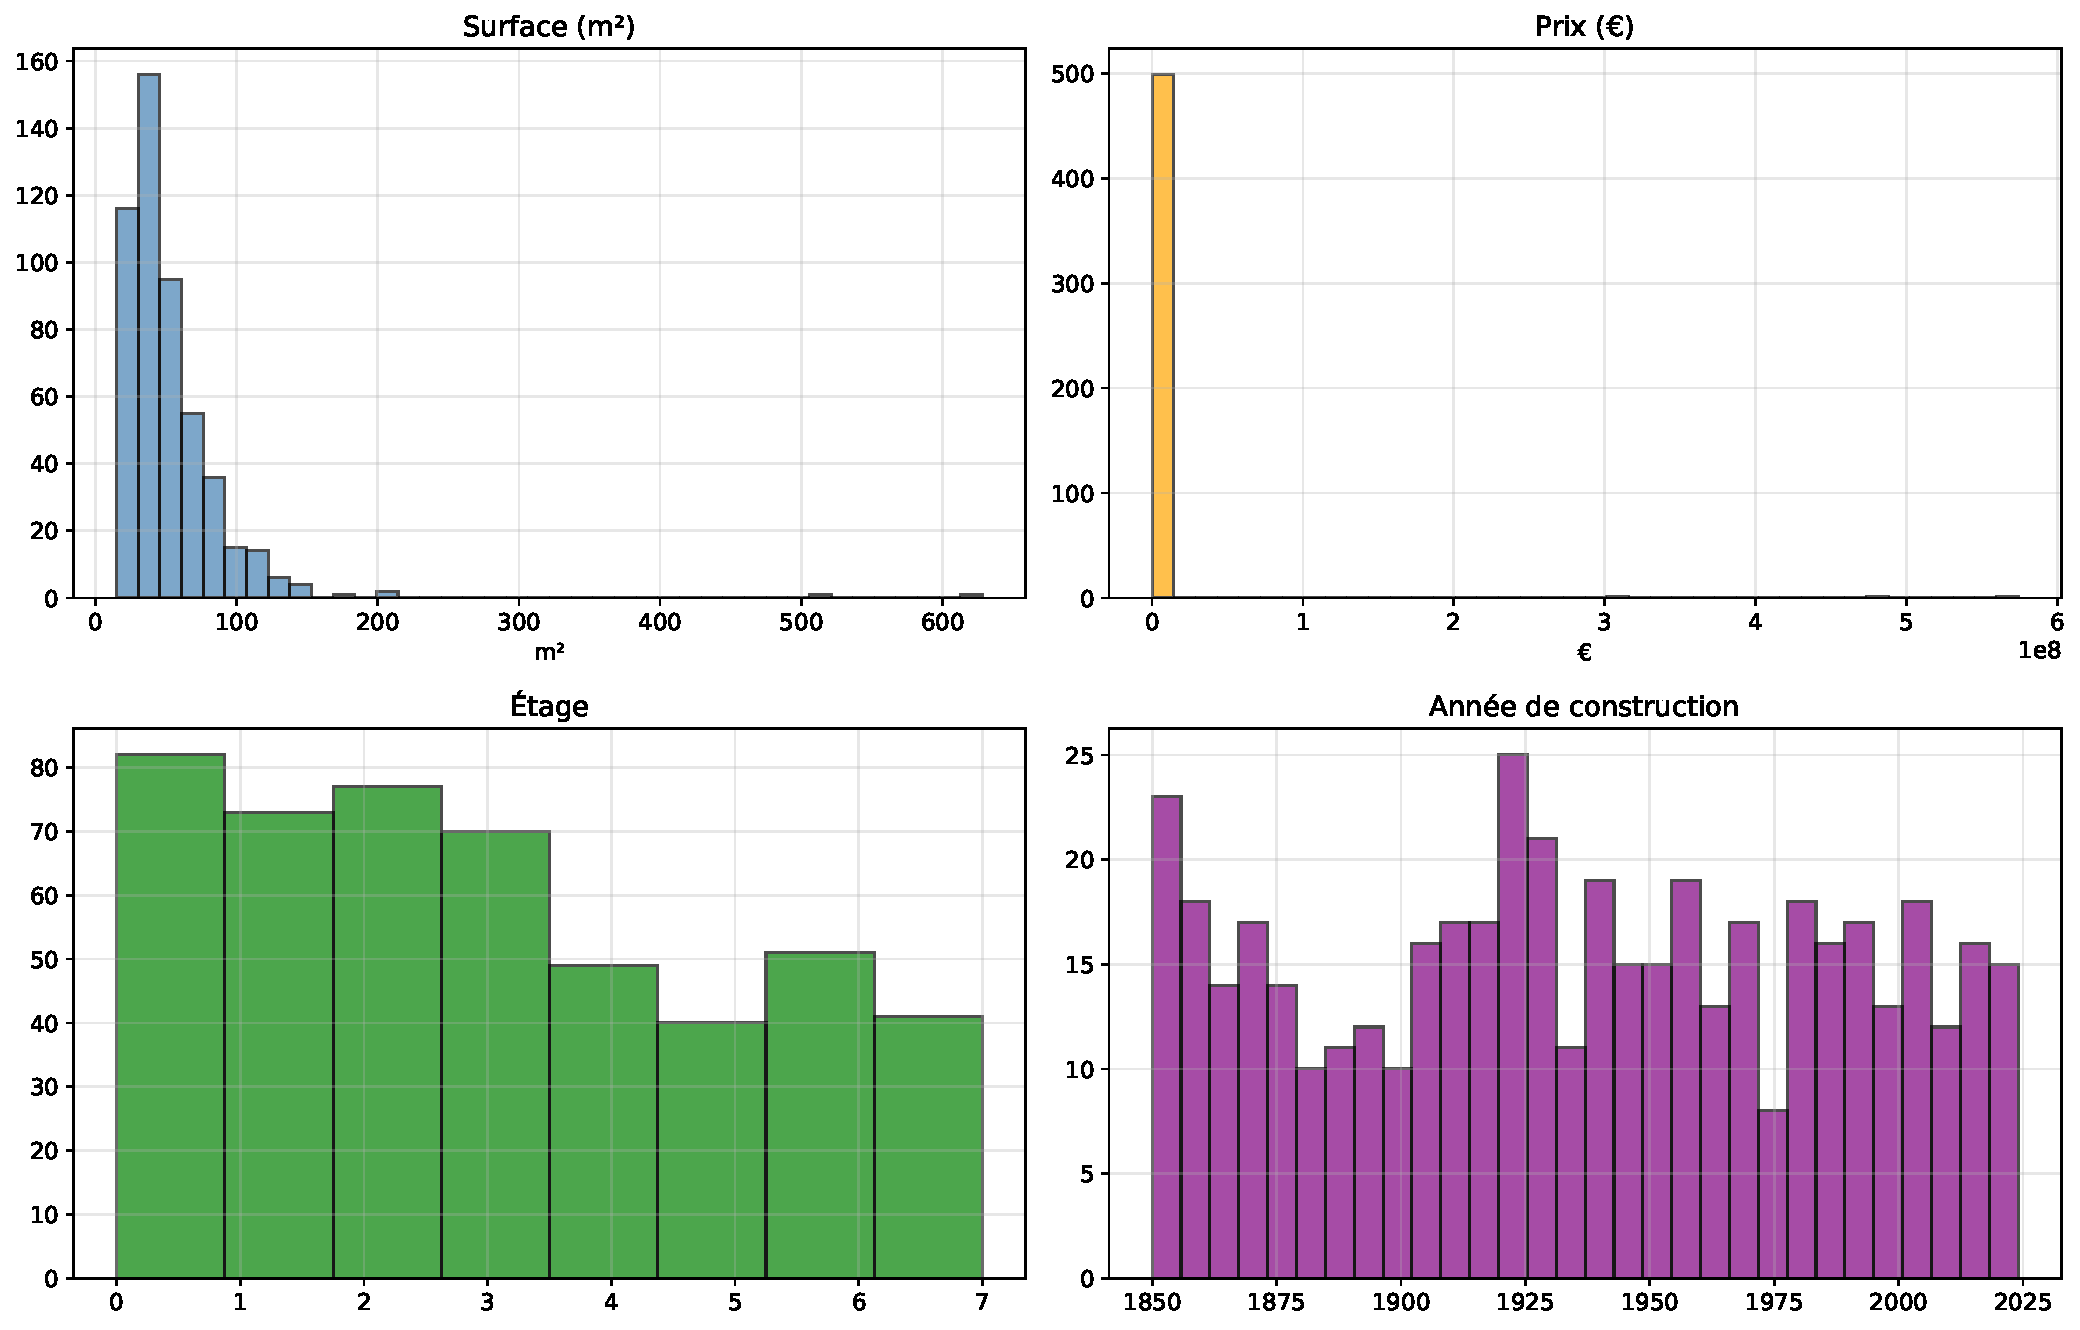
\includegraphics[keepaspectratio]{modules/module_01/tp_sommatif_files/figure-pdf/cell-10-output-1.pdf}}

\textbf{Observations} :

\begin{itemize}
\tightlist
\item
  \texttt{surface\_m2} et \texttt{prix\_eur} ont des
  \textbf{distributions asymétriques à droite} (queue longue avec
  quelques valeurs extrêmes → outliers visuels).
\item
  \texttt{etage} est plutôt uniforme, normal.
\item
  \texttt{annee\_construction} montre des constructions réparties sur
  1850-2024.
\end{itemize}

Les histogrammes confirment les outliers suspectés.

\end{tcolorbox}

\section{✏️ Étape 1.3 --- Étude des
corrélations}\label{uxe9tape-1.3-uxe9tude-des-corruxe9lations}

\begin{tcolorbox}[enhanced jigsaw, arc=.35mm, bottomrule=.15mm, bottomtitle=1mm, breakable, colback=white, colbacktitle=quarto-callout-note-color!10!white, colframe=quarto-callout-note-color-frame, coltitle=black, left=2mm, leftrule=.75mm, opacityback=0, opacitybacktitle=0.6, rightrule=.15mm, title={📝 À faire}, titlerule=0mm, toprule=.15mm, toptitle=1mm]

\begin{enumerate}
\def\labelenumi{\arabic{enumi}.}
\tightlist
\item
  Calcule la \textbf{matrice de corrélation} des variables numériques
  (sans \texttt{prix\_m2} qui fausserait tout).
\item
  Visualise-la avec une \textbf{heatmap} (matplotlib \texttt{imshow} +
  annotations).
\item
  \textbf{Question} : quelles variables sont les plus corrélées au prix
  ?
\end{enumerate}

\end{tcolorbox}

\begin{Shaded}
\begin{Highlighting}[]
\CommentTok{\# }\AlertTok{TODO}\CommentTok{: Étape 1.3}
\end{Highlighting}
\end{Shaded}

\begin{tcolorbox}[enhanced jigsaw, arc=.35mm, bottomrule=.15mm, bottomtitle=1mm, breakable, colback=white, colbacktitle=quarto-callout-tip-color!10!white, colframe=quarto-callout-tip-color-frame, coltitle=black, left=2mm, leftrule=.75mm, opacityback=0, opacitybacktitle=0.6, rightrule=.15mm, title=\textcolor{quarto-callout-tip-color}{\faLightbulb}\hspace{0.5em}{✅ Corrigé Étape 1.3}, titlerule=0mm, toprule=.15mm, toptitle=1mm]

\begin{Shaded}
\begin{Highlighting}[]
\CommentTok{\# Colonnes numériques pertinentes}
\NormalTok{colonnes\_num }\OperatorTok{=}\NormalTok{ [}\StringTok{\textquotesingle{}surface\_m2\textquotesingle{}}\NormalTok{, }\StringTok{\textquotesingle{}nb\_pieces\textquotesingle{}}\NormalTok{, }\StringTok{\textquotesingle{}etage\textquotesingle{}}\NormalTok{, }\StringTok{\textquotesingle{}arrondissement\textquotesingle{}}\NormalTok{,}
                \StringTok{\textquotesingle{}ascenseur\textquotesingle{}}\NormalTok{, }\StringTok{\textquotesingle{}balcon\textquotesingle{}}\NormalTok{, }\StringTok{\textquotesingle{}annee\_construction\textquotesingle{}}\NormalTok{, }\StringTok{\textquotesingle{}prix\_eur\textquotesingle{}}\NormalTok{]}
\NormalTok{matrice\_corr }\OperatorTok{=}\NormalTok{ df[colonnes\_num].corr()}

\CommentTok{\# Visualisation}
\NormalTok{fig, ax }\OperatorTok{=}\NormalTok{ plt.subplots(figsize}\OperatorTok{=}\NormalTok{(}\DecValTok{10}\NormalTok{, }\DecValTok{8}\NormalTok{))}
\NormalTok{im }\OperatorTok{=}\NormalTok{ ax.imshow(matrice\_corr, cmap}\OperatorTok{=}\StringTok{\textquotesingle{}RdBu\_r\textquotesingle{}}\NormalTok{, vmin}\OperatorTok{={-}}\DecValTok{1}\NormalTok{, vmax}\OperatorTok{=}\DecValTok{1}\NormalTok{)}

\CommentTok{\# Ticks}
\NormalTok{ax.set\_xticks(np.arange(}\BuiltInTok{len}\NormalTok{(colonnes\_num)))}
\NormalTok{ax.set\_yticks(np.arange(}\BuiltInTok{len}\NormalTok{(colonnes\_num)))}
\NormalTok{ax.set\_xticklabels(colonnes\_num, rotation}\OperatorTok{=}\DecValTok{45}\NormalTok{, ha}\OperatorTok{=}\StringTok{\textquotesingle{}right\textquotesingle{}}\NormalTok{)}
\NormalTok{ax.set\_yticklabels(colonnes\_num)}

\CommentTok{\# Annotations}
\ControlFlowTok{for}\NormalTok{ i }\KeywordTok{in} \BuiltInTok{range}\NormalTok{(}\BuiltInTok{len}\NormalTok{(colonnes\_num)):}
    \ControlFlowTok{for}\NormalTok{ j }\KeywordTok{in} \BuiltInTok{range}\NormalTok{(}\BuiltInTok{len}\NormalTok{(colonnes\_num)):}
\NormalTok{        ax.text(j, i, }\SpecialStringTok{f"}\SpecialCharTok{\{}\NormalTok{matrice\_corr}\SpecialCharTok{.}\NormalTok{iloc[i, j]}\SpecialCharTok{:.2f\}}\SpecialStringTok{"}\NormalTok{, }
\NormalTok{                ha}\OperatorTok{=}\StringTok{\textquotesingle{}center\textquotesingle{}}\NormalTok{, va}\OperatorTok{=}\StringTok{\textquotesingle{}center\textquotesingle{}}\NormalTok{, fontsize}\OperatorTok{=}\DecValTok{9}\NormalTok{)}

\NormalTok{plt.colorbar(im, ax}\OperatorTok{=}\NormalTok{ax, shrink}\OperatorTok{=}\FloatTok{0.8}\NormalTok{)}
\NormalTok{ax.set\_title(}\StringTok{"Matrice de corrélation (avec outliers)"}\NormalTok{)}
\NormalTok{plt.tight\_layout()}
\NormalTok{plt.show()}

\BuiltInTok{print}\NormalTok{(}\StringTok{"}\CharTok{\textbackslash{}n}\StringTok{Corrélations avec prix\_eur (triées) :"}\NormalTok{)}
\BuiltInTok{print}\NormalTok{(matrice\_corr[}\StringTok{\textquotesingle{}prix\_eur\textquotesingle{}}\NormalTok{].sort\_values(ascending}\OperatorTok{=}\VariableTok{False}\NormalTok{))}
\end{Highlighting}
\end{Shaded}

\pandocbounded{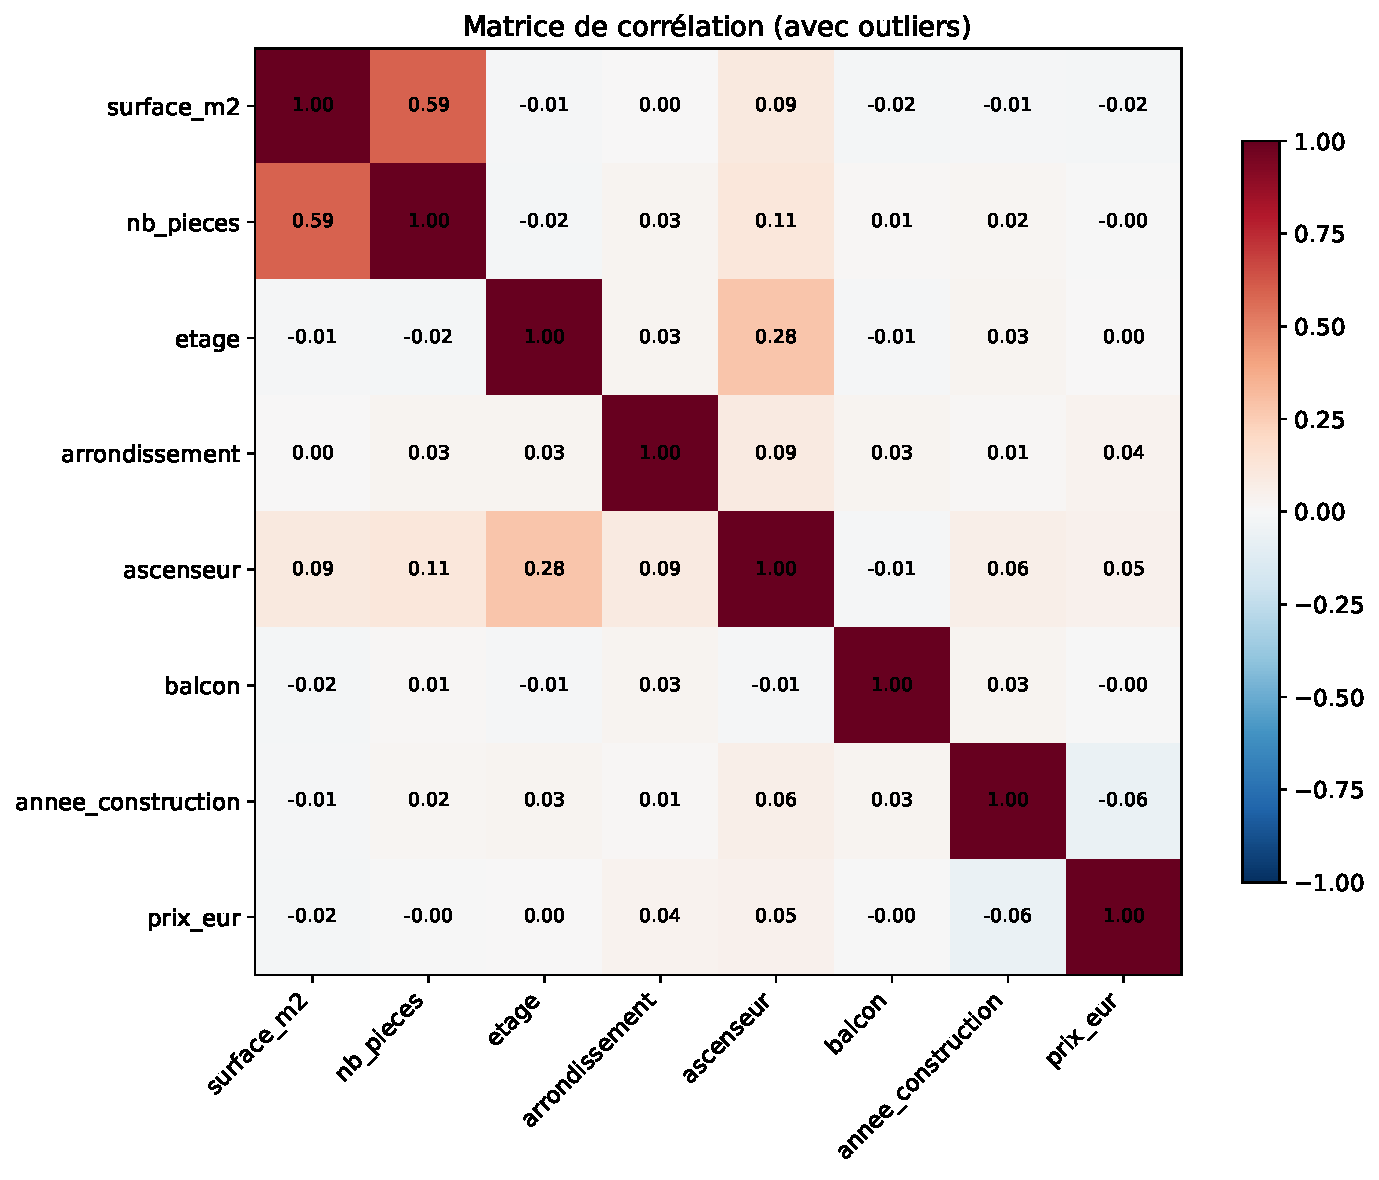
\includegraphics[keepaspectratio]{modules/module_01/tp_sommatif_files/figure-pdf/cell-12-output-1.pdf}}

\begin{verbatim}

Corrélations avec prix_eur (triées) :
prix_eur              1.000000
ascenseur             0.046254
arrondissement        0.037454
etage                 0.001141
nb_pieces            -0.000652
balcon               -0.001156
surface_m2           -0.015953
annee_construction   -0.064715
Name: prix_eur, dtype: float64
\end{verbatim}

\textbf{Observations} :

\begin{itemize}
\tightlist
\item
  \texttt{surface\_m2} a \textbf{la plus forte corrélation} avec le prix
  (logique !).
\item
  \texttt{nb\_pieces} aussi (qui est lui-même corrélé à la surface ---
  on va devoir faire attention au problème de \textbf{colinéarité} plus
  tard).
\item
  \texttt{arrondissement} a une corrélation négative modeste (les
  numéros bas sont plus chers, mais ce n'est pas parfait).
\end{itemize}

⚠️ \textbf{Attention} : ces corrélations sont \textbf{faussées par les
outliers} (notamment les prix aberrants). On les recalculera après
nettoyage.

\end{tcolorbox}

\chapter{Partie 2 --- Nettoyage des
données}\label{partie-2-nettoyage-des-donnuxe9es}

Passons à l'action. On va traiter les problèmes détectés, dans cet ordre
:

\begin{enumerate}
\def\labelenumi{\arabic{enumi}.}
\tightlist
\item
  Doublons
\item
  Colonnes inutiles
\item
  Valeurs manquantes
\item
  Outliers
\item
  Normalisation texte
\end{enumerate}

\section{✏️ Étape 2.1 --- Supprimer les
doublons}\label{uxe9tape-2.1-supprimer-les-doublons}

\begin{tcolorbox}[enhanced jigsaw, arc=.35mm, bottomrule=.15mm, bottomtitle=1mm, breakable, colback=white, colbacktitle=quarto-callout-note-color!10!white, colframe=quarto-callout-note-color-frame, coltitle=black, left=2mm, leftrule=.75mm, opacityback=0, opacitybacktitle=0.6, rightrule=.15mm, title={📝 À faire}, titlerule=0mm, toprule=.15mm, toptitle=1mm]

\begin{enumerate}
\def\labelenumi{\arabic{enumi}.}
\tightlist
\item
  Compte combien il y a de doublons parfaits dans le DataFrame.
\item
  Supprime-les avec \texttt{drop\_duplicates()}.
\item
  Vérifie la nouvelle taille.
\end{enumerate}

\end{tcolorbox}

\begin{Shaded}
\begin{Highlighting}[]
\CommentTok{\# }\AlertTok{TODO}\CommentTok{: Étape 2.1}
\end{Highlighting}
\end{Shaded}

\begin{tcolorbox}[enhanced jigsaw, arc=.35mm, bottomrule=.15mm, bottomtitle=1mm, breakable, colback=white, colbacktitle=quarto-callout-tip-color!10!white, colframe=quarto-callout-tip-color-frame, coltitle=black, left=2mm, leftrule=.75mm, opacityback=0, opacitybacktitle=0.6, rightrule=.15mm, title=\textcolor{quarto-callout-tip-color}{\faLightbulb}\hspace{0.5em}{✅ Corrigé Étape 2.1}, titlerule=0mm, toprule=.15mm, toptitle=1mm]

\begin{Shaded}
\begin{Highlighting}[]
\NormalTok{n\_doublons }\OperatorTok{=}\NormalTok{ df.duplicated().}\BuiltInTok{sum}\NormalTok{()}
\BuiltInTok{print}\NormalTok{(}\SpecialStringTok{f"Doublons détectés : }\SpecialCharTok{\{}\NormalTok{n\_doublons}\SpecialCharTok{\}}\SpecialStringTok{"}\NormalTok{)}

\NormalTok{df }\OperatorTok{=}\NormalTok{ df.drop\_duplicates().reset\_index(drop}\OperatorTok{=}\VariableTok{True}\NormalTok{)}
\BuiltInTok{print}\NormalTok{(}\SpecialStringTok{f"Nouvelle taille : }\SpecialCharTok{\{}\BuiltInTok{len}\NormalTok{(df)}\SpecialCharTok{\}}\SpecialStringTok{ lignes"}\NormalTok{)}
\end{Highlighting}
\end{Shaded}

\begin{verbatim}
Doublons détectés : 1
Nouvelle taille : 501 lignes
\end{verbatim}

\end{tcolorbox}

\section{✏️ Étape 2.2 --- Supprimer les colonnes
inutiles}\label{uxe9tape-2.2-supprimer-les-colonnes-inutiles}

\begin{tcolorbox}[enhanced jigsaw, arc=.35mm, bottomrule=.15mm, bottomtitle=1mm, breakable, colback=white, colbacktitle=quarto-callout-note-color!10!white, colframe=quarto-callout-note-color-frame, coltitle=black, left=2mm, leftrule=.75mm, opacityback=0, opacitybacktitle=0.6, rightrule=.15mm, title={📝 À faire}, titlerule=0mm, toprule=.15mm, toptitle=1mm]

Deux colonnes posent problème :

\begin{itemize}
\tightlist
\item
  \texttt{prix\_m2} est \textbf{redondante} (= prix\_eur / surface\_m2)
  et créerait une fuite de données dans le modèle
\item
  \texttt{type\_bien} est \textbf{inutile} (toutes les valeurs désignent
  un appartement, juste mal écrit)
\end{itemize}

Supprime-les.

\end{tcolorbox}

\begin{Shaded}
\begin{Highlighting}[]
\CommentTok{\# }\AlertTok{TODO}\CommentTok{: Étape 2.2}
\end{Highlighting}
\end{Shaded}

\begin{tcolorbox}[enhanced jigsaw, arc=.35mm, bottomrule=.15mm, bottomtitle=1mm, breakable, colback=white, colbacktitle=quarto-callout-tip-color!10!white, colframe=quarto-callout-tip-color-frame, coltitle=black, left=2mm, leftrule=.75mm, opacityback=0, opacitybacktitle=0.6, rightrule=.15mm, title=\textcolor{quarto-callout-tip-color}{\faLightbulb}\hspace{0.5em}{✅ Corrigé Étape 2.2}, titlerule=0mm, toprule=.15mm, toptitle=1mm]

\begin{Shaded}
\begin{Highlighting}[]
\NormalTok{df }\OperatorTok{=}\NormalTok{ df.drop(columns}\OperatorTok{=}\NormalTok{[}\StringTok{\textquotesingle{}prix\_m2\textquotesingle{}}\NormalTok{, }\StringTok{\textquotesingle{}type\_bien\textquotesingle{}}\NormalTok{])}
\BuiltInTok{print}\NormalTok{(}\SpecialStringTok{f"Colonnes restantes : }\SpecialCharTok{\{}\NormalTok{df}\SpecialCharTok{.}\NormalTok{columns}\SpecialCharTok{.}\NormalTok{tolist()}\SpecialCharTok{\}}\SpecialStringTok{"}\NormalTok{)}
\end{Highlighting}
\end{Shaded}

\begin{verbatim}
Colonnes restantes : ['surface_m2', 'nb_pieces', 'etage', 'arrondissement', 'ascenseur', 'balcon', 'annee_construction', 'prix_eur']
\end{verbatim}

\textbf{Pourquoi supprimer \texttt{prix\_m2} ?}\\
Parce que si on laissait cette colonne, notre modèle « apprendrait » à
prédire le prix depuis le prix au m², ce qui est de la triche (fuite de
données = \textbf{data leakage}). En pratique, on ne connaît pas le prix
au m² AVANT de prédire le prix !

\end{tcolorbox}

\section{✏️ Étape 2.3 --- Traiter les valeurs
manquantes}\label{uxe9tape-2.3-traiter-les-valeurs-manquantes}

\begin{tcolorbox}[enhanced jigsaw, arc=.35mm, bottomrule=.15mm, bottomtitle=1mm, breakable, colback=white, colbacktitle=quarto-callout-note-color!10!white, colframe=quarto-callout-note-color-frame, coltitle=black, left=2mm, leftrule=.75mm, opacityback=0, opacitybacktitle=0.6, rightrule=.15mm, title={📝 À faire}, titlerule=0mm, toprule=.15mm, toptitle=1mm]

\begin{enumerate}
\def\labelenumi{\arabic{enumi}.}
\tightlist
\item
  Compte les valeurs manquantes par colonne.
\item
  \textbf{Choisis une stratégie} pour chacune :

  \begin{itemize}
  \tightlist
  \item
    \texttt{etage} : imputer avec la \textbf{médiane} (c'est une
    variable discrète)
  \item
    \texttt{balcon} : imputer avec \textbf{0} (on suppose qu'absence =
    pas de balcon)
  \item
    \texttt{annee\_construction} : imputer avec la \textbf{médiane}
  \end{itemize}
\item
  Vérifie qu'il n'y a plus de NaN.
\end{enumerate}

\end{tcolorbox}

\begin{Shaded}
\begin{Highlighting}[]
\CommentTok{\# }\AlertTok{TODO}\CommentTok{: Étape 2.3}
\end{Highlighting}
\end{Shaded}

\begin{tcolorbox}[enhanced jigsaw, arc=.35mm, bottomrule=.15mm, bottomtitle=1mm, breakable, colback=white, colbacktitle=quarto-callout-tip-color!10!white, colframe=quarto-callout-tip-color-frame, coltitle=black, left=2mm, leftrule=.75mm, opacityback=0, opacitybacktitle=0.6, rightrule=.15mm, title=\textcolor{quarto-callout-tip-color}{\faLightbulb}\hspace{0.5em}{✅ Corrigé Étape 2.3}, titlerule=0mm, toprule=.15mm, toptitle=1mm]

\begin{Shaded}
\begin{Highlighting}[]
\CommentTok{\# 1. Compte des NaN}
\BuiltInTok{print}\NormalTok{(}\StringTok{"Valeurs manquantes avant :"}\NormalTok{)}
\BuiltInTok{print}\NormalTok{(df.isna().}\BuiltInTok{sum}\NormalTok{())}

\CommentTok{\# 2. Imputation}
\NormalTok{df[}\StringTok{\textquotesingle{}etage\textquotesingle{}}\NormalTok{] }\OperatorTok{=}\NormalTok{ df[}\StringTok{\textquotesingle{}etage\textquotesingle{}}\NormalTok{].fillna(df[}\StringTok{\textquotesingle{}etage\textquotesingle{}}\NormalTok{].median())}
\NormalTok{df[}\StringTok{\textquotesingle{}balcon\textquotesingle{}}\NormalTok{] }\OperatorTok{=}\NormalTok{ df[}\StringTok{\textquotesingle{}balcon\textquotesingle{}}\NormalTok{].fillna(}\DecValTok{0}\NormalTok{).astype(}\BuiltInTok{int}\NormalTok{)}
\NormalTok{df[}\StringTok{\textquotesingle{}annee\_construction\textquotesingle{}}\NormalTok{] }\OperatorTok{=}\NormalTok{ df[}\StringTok{\textquotesingle{}annee\_construction\textquotesingle{}}\NormalTok{].fillna(df[}\StringTok{\textquotesingle{}annee\_construction\textquotesingle{}}\NormalTok{].median())}

\CommentTok{\# 3. Vérification}
\BuiltInTok{print}\NormalTok{(}\StringTok{"}\CharTok{\textbackslash{}n}\StringTok{Valeurs manquantes après :"}\NormalTok{)}
\BuiltInTok{print}\NormalTok{(df.isna().}\BuiltInTok{sum}\NormalTok{())}
\end{Highlighting}
\end{Shaded}

\begin{verbatim}
Valeurs manquantes avant :
surface_m2             0
nb_pieces              0
etage                 19
arrondissement         0
ascenseur              0
balcon                33
annee_construction    34
prix_eur               0
dtype: int64

Valeurs manquantes après :
surface_m2            0
nb_pieces             0
etage                 0
arrondissement        0
ascenseur             0
balcon                0
annee_construction    0
prix_eur              0
dtype: int64
\end{verbatim}

\textbf{Important} : il y a d'autres stratégies possibles (supprimer les
lignes, imputer avec une régression, etc.). Pour ce TP on reste simples.
Mais dans un vrai projet, \textbf{justifie toujours ton choix}
d'imputation.

\end{tcolorbox}

\section{✏️ Étape 2.4 --- Détecter et traiter les
outliers}\label{uxe9tape-2.4-duxe9tecter-et-traiter-les-outliers}

\begin{tcolorbox}[enhanced jigsaw, arc=.35mm, bottomrule=.15mm, bottomtitle=1mm, breakable, colback=white, colbacktitle=quarto-callout-note-color!10!white, colframe=quarto-callout-note-color-frame, coltitle=black, left=2mm, leftrule=.75mm, opacityback=0, opacitybacktitle=0.6, rightrule=.15mm, title={📝 À faire}, titlerule=0mm, toprule=.15mm, toptitle=1mm]

On va utiliser la méthode IQR vue en Notion 1.3.

\begin{enumerate}
\def\labelenumi{\arabic{enumi}.}
\tightlist
\item
  Pour \texttt{surface\_m2}, calcule Q1, Q3, IQR et les bornes
  \texttt{{[}Q1\ -\ 1.5×IQR,\ Q3\ +\ 1.5×IQR{]}}.
\item
  Identifie les lignes hors bornes.
\item
  Fais pareil pour \texttt{prix\_eur}.
\item
  \textbf{Supprime} les lignes qui sont outliers sur l'une ou l'autre
  variable.
\item
  Affiche combien de lignes ont été supprimées.
\end{enumerate}

\end{tcolorbox}

\begin{Shaded}
\begin{Highlighting}[]
\CommentTok{\# }\AlertTok{TODO}\CommentTok{: Étape 2.4}
\end{Highlighting}
\end{Shaded}

\begin{tcolorbox}[enhanced jigsaw, arc=.35mm, bottomrule=.15mm, bottomtitle=1mm, breakable, colback=white, colbacktitle=quarto-callout-tip-color!10!white, colframe=quarto-callout-tip-color-frame, coltitle=black, left=2mm, leftrule=.75mm, opacityback=0, opacitybacktitle=0.6, rightrule=.15mm, title=\textcolor{quarto-callout-tip-color}{\faLightbulb}\hspace{0.5em}{✅ Corrigé Étape 2.4}, titlerule=0mm, toprule=.15mm, toptitle=1mm]

\begin{Shaded}
\begin{Highlighting}[]
\NormalTok{taille\_avant }\OperatorTok{=} \BuiltInTok{len}\NormalTok{(df)}

\CommentTok{\# Fonction utilitaire}
\KeywordTok{def}\NormalTok{ detecter\_outliers\_iqr(serie):}
\NormalTok{    q1 }\OperatorTok{=}\NormalTok{ serie.quantile(}\FloatTok{0.25}\NormalTok{)}
\NormalTok{    q3 }\OperatorTok{=}\NormalTok{ serie.quantile(}\FloatTok{0.75}\NormalTok{)}
\NormalTok{    iqr }\OperatorTok{=}\NormalTok{ q3 }\OperatorTok{{-}}\NormalTok{ q1}
\NormalTok{    borne\_basse }\OperatorTok{=}\NormalTok{ q1 }\OperatorTok{{-}} \FloatTok{1.5} \OperatorTok{*}\NormalTok{ iqr}
\NormalTok{    borne\_haute }\OperatorTok{=}\NormalTok{ q3 }\OperatorTok{+} \FloatTok{1.5} \OperatorTok{*}\NormalTok{ iqr}
    \ControlFlowTok{return}\NormalTok{ (serie }\OperatorTok{\textless{}}\NormalTok{ borne\_basse) }\OperatorTok{|}\NormalTok{ (serie }\OperatorTok{\textgreater{}}\NormalTok{ borne\_haute)}

\CommentTok{\# Détection sur surface et prix}
\NormalTok{outliers\_surface }\OperatorTok{=}\NormalTok{ detecter\_outliers\_iqr(df[}\StringTok{\textquotesingle{}surface\_m2\textquotesingle{}}\NormalTok{])}
\NormalTok{outliers\_prix }\OperatorTok{=}\NormalTok{ detecter\_outliers\_iqr(df[}\StringTok{\textquotesingle{}prix\_eur\textquotesingle{}}\NormalTok{])}

\BuiltInTok{print}\NormalTok{(}\SpecialStringTok{f"Outliers surface\_m2 : }\SpecialCharTok{\{}\NormalTok{outliers\_surface}\SpecialCharTok{.}\BuiltInTok{sum}\NormalTok{()}\SpecialCharTok{\}}\SpecialStringTok{"}\NormalTok{)}
\BuiltInTok{print}\NormalTok{(}\SpecialStringTok{f"Outliers prix\_eur   : }\SpecialCharTok{\{}\NormalTok{outliers\_prix}\SpecialCharTok{.}\BuiltInTok{sum}\NormalTok{()}\SpecialCharTok{\}}\SpecialStringTok{"}\NormalTok{)}

\CommentTok{\# Supprimer les lignes outliers (sur l\textquotesingle{}une OU l\textquotesingle{}autre variable)}
\NormalTok{df }\OperatorTok{=}\NormalTok{ df[}\OperatorTok{\textasciitilde{}}\NormalTok{(outliers\_surface }\OperatorTok{|}\NormalTok{ outliers\_prix)].reset\_index(drop}\OperatorTok{=}\VariableTok{True}\NormalTok{)}

\BuiltInTok{print}\NormalTok{(}\SpecialStringTok{f"}\CharTok{\textbackslash{}n}\SpecialStringTok{Lignes supprimées : }\SpecialCharTok{\{}\NormalTok{taille\_avant }\OperatorTok{{-}} \BuiltInTok{len}\NormalTok{(df)}\SpecialCharTok{\}}\SpecialStringTok{"}\NormalTok{)}
\BuiltInTok{print}\NormalTok{(}\SpecialStringTok{f"Taille finale : }\SpecialCharTok{\{}\BuiltInTok{len}\NormalTok{(df)}\SpecialCharTok{\}}\SpecialStringTok{ lignes"}\NormalTok{)}
\end{Highlighting}
\end{Shaded}

\begin{verbatim}
Outliers surface_m2 : 23
Outliers prix_eur   : 26

Lignes supprimées : 34
Taille finale : 467 lignes
\end{verbatim}

\begin{quote}
\textbf{Note}

\textbf{Nuance importante} : en pratique, on ne supprime pas toujours
les outliers. Parfois ils sont intéressants (ex : fraude bancaire). Ici
on les supprime parce qu'on a identifié que ce sont des \textbf{erreurs
de saisie}.
\end{quote}

\end{tcolorbox}

\section{✏️ Étape 2.5 --- Vérification
post-nettoyage}\label{uxe9tape-2.5-vuxe9rification-post-nettoyage}

\begin{tcolorbox}[enhanced jigsaw, arc=.35mm, bottomrule=.15mm, bottomtitle=1mm, breakable, colback=white, colbacktitle=quarto-callout-note-color!10!white, colframe=quarto-callout-note-color-frame, coltitle=black, left=2mm, leftrule=.75mm, opacityback=0, opacitybacktitle=0.6, rightrule=.15mm, title={📝 À faire}, titlerule=0mm, toprule=.15mm, toptitle=1mm]

Compare \textbf{avant/après nettoyage} :

\begin{itemize}
\tightlist
\item
  Retrace l'histogramme de \texttt{prix\_eur} et \texttt{surface\_m2}.
\item
  Recalcule la matrice de corrélation.
\item
  Les corrélations ont-elles changé significativement ?
\end{itemize}

\end{tcolorbox}

\begin{Shaded}
\begin{Highlighting}[]
\CommentTok{\# }\AlertTok{TODO}\CommentTok{: Étape 2.5}
\end{Highlighting}
\end{Shaded}

\begin{tcolorbox}[enhanced jigsaw, arc=.35mm, bottomrule=.15mm, bottomtitle=1mm, breakable, colback=white, colbacktitle=quarto-callout-tip-color!10!white, colframe=quarto-callout-tip-color-frame, coltitle=black, left=2mm, leftrule=.75mm, opacityback=0, opacitybacktitle=0.6, rightrule=.15mm, title=\textcolor{quarto-callout-tip-color}{\faLightbulb}\hspace{0.5em}{✅ Corrigé Étape 2.5}, titlerule=0mm, toprule=.15mm, toptitle=1mm]

\begin{Shaded}
\begin{Highlighting}[]
\NormalTok{fig, axes }\OperatorTok{=}\NormalTok{ plt.subplots(}\DecValTok{1}\NormalTok{, }\DecValTok{2}\NormalTok{, figsize}\OperatorTok{=}\NormalTok{(}\DecValTok{13}\NormalTok{, }\DecValTok{4}\NormalTok{))}

\NormalTok{axes[}\DecValTok{0}\NormalTok{].hist(df[}\StringTok{\textquotesingle{}surface\_m2\textquotesingle{}}\NormalTok{], bins}\OperatorTok{=}\DecValTok{40}\NormalTok{, color}\OperatorTok{=}\StringTok{\textquotesingle{}steelblue\textquotesingle{}}\NormalTok{, edgecolor}\OperatorTok{=}\StringTok{\textquotesingle{}black\textquotesingle{}}\NormalTok{, alpha}\OperatorTok{=}\FloatTok{0.7}\NormalTok{)}
\NormalTok{axes[}\DecValTok{0}\NormalTok{].set\_title(}\StringTok{\textquotesingle{}Surface APRÈS nettoyage\textquotesingle{}}\NormalTok{)}
\NormalTok{axes[}\DecValTok{0}\NormalTok{].set\_xlabel(}\StringTok{\textquotesingle{}m²\textquotesingle{}}\NormalTok{)}
\NormalTok{axes[}\DecValTok{0}\NormalTok{].grid(}\VariableTok{True}\NormalTok{, alpha}\OperatorTok{=}\FloatTok{0.3}\NormalTok{)}

\NormalTok{axes[}\DecValTok{1}\NormalTok{].hist(df[}\StringTok{\textquotesingle{}prix\_eur\textquotesingle{}}\NormalTok{], bins}\OperatorTok{=}\DecValTok{40}\NormalTok{, color}\OperatorTok{=}\StringTok{\textquotesingle{}orange\textquotesingle{}}\NormalTok{, edgecolor}\OperatorTok{=}\StringTok{\textquotesingle{}black\textquotesingle{}}\NormalTok{, alpha}\OperatorTok{=}\FloatTok{0.7}\NormalTok{)}
\NormalTok{axes[}\DecValTok{1}\NormalTok{].set\_title(}\StringTok{\textquotesingle{}Prix APRÈS nettoyage\textquotesingle{}}\NormalTok{)}
\NormalTok{axes[}\DecValTok{1}\NormalTok{].set\_xlabel(}\StringTok{\textquotesingle{}€\textquotesingle{}}\NormalTok{)}
\NormalTok{axes[}\DecValTok{1}\NormalTok{].grid(}\VariableTok{True}\NormalTok{, alpha}\OperatorTok{=}\FloatTok{0.3}\NormalTok{)}

\NormalTok{plt.tight\_layout()}
\NormalTok{plt.show()}

\CommentTok{\# Matrice de corrélation propre}
\NormalTok{matrice\_corr\_clean }\OperatorTok{=}\NormalTok{ df.corr()}
\BuiltInTok{print}\NormalTok{(}\StringTok{"}\CharTok{\textbackslash{}n}\StringTok{Corrélations avec prix\_eur (après nettoyage) :"}\NormalTok{)}
\BuiltInTok{print}\NormalTok{(matrice\_corr\_clean[}\StringTok{\textquotesingle{}prix\_eur\textquotesingle{}}\NormalTok{].sort\_values(ascending}\OperatorTok{=}\VariableTok{False}\NormalTok{))}
\end{Highlighting}
\end{Shaded}

\pandocbounded{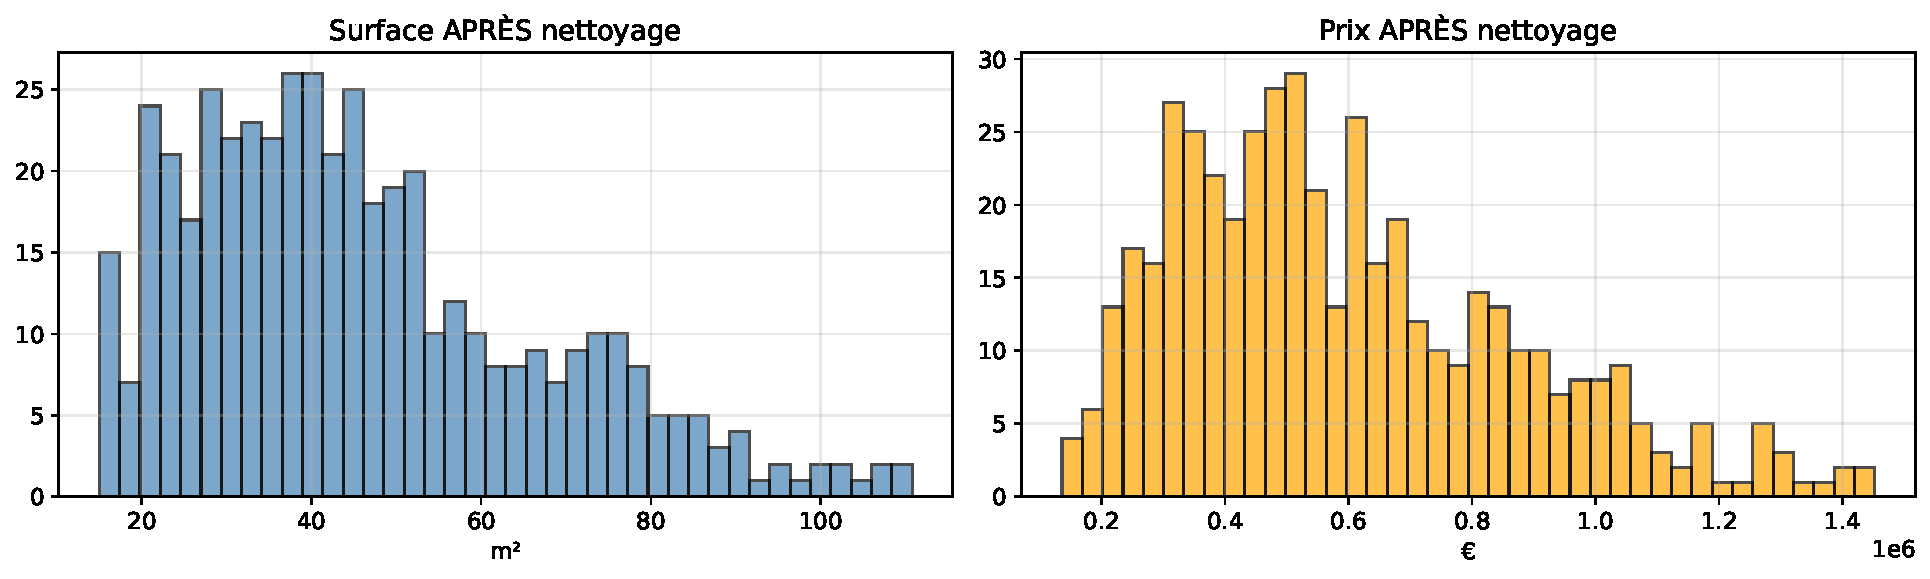
\includegraphics[keepaspectratio]{modules/module_01/tp_sommatif_files/figure-pdf/cell-22-output-1.pdf}}

\begin{verbatim}

Corrélations avec prix_eur (après nettoyage) :
prix_eur              1.000000
surface_m2            0.879940
nb_pieces             0.780293
ascenseur             0.137007
etage                 0.109710
annee_construction    0.086657
balcon                0.037700
arrondissement       -0.209316
Name: prix_eur, dtype: float64
\end{verbatim}

\textbf{Observation attendue} : sans les outliers, les distributions
redeviennent plus lisibles, et les corrélations sont plus fortes et plus
fiables (les outliers tiraient les corrélations dans tous les sens).

\end{tcolorbox}

\chapter{Partie 3 --- Préparation pour le
ML}\label{partie-3-pruxe9paration-pour-le-ml}

\section{🎯 Objectif}\label{objectif-1}

Mettre les données sous une forme exploitable par notre algorithme de
descente de gradient.

\section{✏️ Étape 3.1 --- Séparer X et
y}\label{uxe9tape-3.1-suxe9parer-x-et-y}

\begin{tcolorbox}[enhanced jigsaw, arc=.35mm, bottomrule=.15mm, bottomtitle=1mm, breakable, colback=white, colbacktitle=quarto-callout-note-color!10!white, colframe=quarto-callout-note-color-frame, coltitle=black, left=2mm, leftrule=.75mm, opacityback=0, opacitybacktitle=0.6, rightrule=.15mm, title={📝 À faire}, titlerule=0mm, toprule=.15mm, toptitle=1mm]

\begin{enumerate}
\def\labelenumi{\arabic{enumi}.}
\tightlist
\item
  Crée \texttt{X} : la matrice des \textbf{variables explicatives}
  (toutes sauf \texttt{prix\_eur}).
\item
  Crée \texttt{y} : le \textbf{vecteur cible} (\texttt{prix\_eur}).
\item
  Convertis-les en arrays NumPy.
\item
  Affiche leurs dimensions.
\end{enumerate}

\end{tcolorbox}

\begin{Shaded}
\begin{Highlighting}[]
\CommentTok{\# }\AlertTok{TODO}\CommentTok{: Étape 3.1}
\end{Highlighting}
\end{Shaded}

\begin{tcolorbox}[enhanced jigsaw, arc=.35mm, bottomrule=.15mm, bottomtitle=1mm, breakable, colback=white, colbacktitle=quarto-callout-tip-color!10!white, colframe=quarto-callout-tip-color-frame, coltitle=black, left=2mm, leftrule=.75mm, opacityback=0, opacitybacktitle=0.6, rightrule=.15mm, title=\textcolor{quarto-callout-tip-color}{\faLightbulb}\hspace{0.5em}{✅ Corrigé Étape 3.1}, titlerule=0mm, toprule=.15mm, toptitle=1mm]

\begin{Shaded}
\begin{Highlighting}[]
\CommentTok{\# Features et target}
\NormalTok{feature\_names }\OperatorTok{=}\NormalTok{ [c }\ControlFlowTok{for}\NormalTok{ c }\KeywordTok{in}\NormalTok{ df.columns }\ControlFlowTok{if}\NormalTok{ c }\OperatorTok{!=} \StringTok{\textquotesingle{}prix\_eur\textquotesingle{}}\NormalTok{]}
\NormalTok{X }\OperatorTok{=}\NormalTok{ df[feature\_names].values.astype(}\BuiltInTok{float}\NormalTok{)}
\NormalTok{y }\OperatorTok{=}\NormalTok{ df[}\StringTok{\textquotesingle{}prix\_eur\textquotesingle{}}\NormalTok{].values.astype(}\BuiltInTok{float}\NormalTok{)}

\BuiltInTok{print}\NormalTok{(}\SpecialStringTok{f"X shape : }\SpecialCharTok{\{}\NormalTok{X}\SpecialCharTok{.}\NormalTok{shape}\SpecialCharTok{\}}\SpecialStringTok{"}\NormalTok{)  }\CommentTok{\# (n\_echantillons, n\_features)}
\BuiltInTok{print}\NormalTok{(}\SpecialStringTok{f"y shape : }\SpecialCharTok{\{}\NormalTok{y}\SpecialCharTok{.}\NormalTok{shape}\SpecialCharTok{\}}\SpecialStringTok{"}\NormalTok{)}
\BuiltInTok{print}\NormalTok{(}\SpecialStringTok{f"Features utilisées : }\SpecialCharTok{\{}\NormalTok{feature\_names}\SpecialCharTok{\}}\SpecialStringTok{"}\NormalTok{)}
\end{Highlighting}
\end{Shaded}

\begin{verbatim}
X shape : (467, 7)
y shape : (467,)
Features utilisées : ['surface_m2', 'nb_pieces', 'etage', 'arrondissement', 'ascenseur', 'balcon', 'annee_construction']
\end{verbatim}

\end{tcolorbox}

\section{✏️ Étape 3.2 --- Séparer train et
test}\label{uxe9tape-3.2-suxe9parer-train-et-test}

\begin{tcolorbox}[enhanced jigsaw, arc=.35mm, bottomrule=.15mm, bottomtitle=1mm, breakable, colback=white, colbacktitle=quarto-callout-note-color!10!white, colframe=quarto-callout-note-color-frame, coltitle=black, left=2mm, leftrule=.75mm, opacityback=0, opacitybacktitle=0.6, rightrule=.15mm, title={📝 À faire}, titlerule=0mm, toprule=.15mm, toptitle=1mm]

Pour évaluer honnêtement notre modèle, on doit le tester sur des données
\textbf{qu'il n'a pas vues pendant l'entraînement}.

\begin{enumerate}
\def\labelenumi{\arabic{enumi}.}
\tightlist
\item
  Mélange les indices aléatoirement avec \texttt{np.random.permutation}.
\item
  Garde \textbf{80\% pour l'entraînement} et \textbf{20\% pour le test}.
\item
  Crée \texttt{X\_train}, \texttt{X\_test}, \texttt{y\_train},
  \texttt{y\_test}.
\end{enumerate}

\end{tcolorbox}

\begin{Shaded}
\begin{Highlighting}[]
\CommentTok{\# }\AlertTok{TODO}\CommentTok{: Étape 3.2}
\end{Highlighting}
\end{Shaded}

\begin{tcolorbox}[enhanced jigsaw, arc=.35mm, bottomrule=.15mm, bottomtitle=1mm, breakable, colback=white, colbacktitle=quarto-callout-tip-color!10!white, colframe=quarto-callout-tip-color-frame, coltitle=black, left=2mm, leftrule=.75mm, opacityback=0, opacitybacktitle=0.6, rightrule=.15mm, title=\textcolor{quarto-callout-tip-color}{\faLightbulb}\hspace{0.5em}{✅ Corrigé Étape 3.2}, titlerule=0mm, toprule=.15mm, toptitle=1mm]

\begin{Shaded}
\begin{Highlighting}[]
\NormalTok{np.random.seed(}\DecValTok{42}\NormalTok{)}

\CommentTok{\# Mélange}
\NormalTok{n }\OperatorTok{=} \BuiltInTok{len}\NormalTok{(X)}
\NormalTok{indices }\OperatorTok{=}\NormalTok{ np.random.permutation(n)}
\NormalTok{n\_train }\OperatorTok{=} \BuiltInTok{int}\NormalTok{(}\FloatTok{0.8} \OperatorTok{*}\NormalTok{ n)}

\NormalTok{indices\_train }\OperatorTok{=}\NormalTok{ indices[:n\_train]}
\NormalTok{indices\_test }\OperatorTok{=}\NormalTok{ indices[n\_train:]}

\NormalTok{X\_train }\OperatorTok{=}\NormalTok{ X[indices\_train]}
\NormalTok{X\_test }\OperatorTok{=}\NormalTok{ X[indices\_test]}
\NormalTok{y\_train }\OperatorTok{=}\NormalTok{ y[indices\_train]}
\NormalTok{y\_test }\OperatorTok{=}\NormalTok{ y[indices\_test]}

\BuiltInTok{print}\NormalTok{(}\SpecialStringTok{f"Train : }\SpecialCharTok{\{}\BuiltInTok{len}\NormalTok{(X\_train)}\SpecialCharTok{\}}\SpecialStringTok{ échantillons"}\NormalTok{)}
\BuiltInTok{print}\NormalTok{(}\SpecialStringTok{f"Test  : }\SpecialCharTok{\{}\BuiltInTok{len}\NormalTok{(X\_test)}\SpecialCharTok{\}}\SpecialStringTok{ échantillons"}\NormalTok{)}
\end{Highlighting}
\end{Shaded}

\begin{verbatim}
Train : 373 échantillons
Test  : 94 échantillons
\end{verbatim}

\begin{quote}
\textbf{🧠 Règle d'or}

\textbf{Ne jamais utiliser les données de test pendant l'entraînement.}
Si tu regardes le test pour ajuster ton modèle, tu triches --- et tes
scores seront trompeurs. Le test, c'est l'examen final.
\end{quote}

\end{tcolorbox}

\section{✏️ Étape 3.3 --- Normaliser les
features}\label{uxe9tape-3.3-normaliser-les-features}

\begin{tcolorbox}[enhanced jigsaw, arc=.35mm, bottomrule=.15mm, bottomtitle=1mm, breakable, colback=white, colbacktitle=quarto-callout-note-color!10!white, colframe=quarto-callout-note-color-frame, coltitle=black, left=2mm, leftrule=.75mm, opacityback=0, opacitybacktitle=0.6, rightrule=.15mm, title={📝 À faire}, titlerule=0mm, toprule=.15mm, toptitle=1mm]

Comme vu en Notion 1.2, la descente de gradient marche beaucoup mieux
avec des variables normalisées (moyenne 0, écart-type 1).

\textbf{Attention subtile} : tu dois calculer moyenne et écart-type
\textbf{uniquement sur les données d'entraînement}, puis appliquer la
même transformation aux données de test.

\begin{enumerate}
\def\labelenumi{\arabic{enumi}.}
\tightlist
\item
  Calcule \texttt{X\_train\_mean} et \texttt{X\_train\_std}.
\item
  Normalise \texttt{X\_train} → \texttt{X\_train\_norm}.
\item
  Normalise \texttt{X\_test} avec les \textbf{mêmes moyenne et
  écart-type} → \texttt{X\_test\_norm}.
\item
  Normalise aussi \texttt{y\_train} et \texttt{y\_test}.
\end{enumerate}

\end{tcolorbox}

\begin{Shaded}
\begin{Highlighting}[]
\CommentTok{\# }\AlertTok{TODO}\CommentTok{: Étape 3.3}
\end{Highlighting}
\end{Shaded}

\begin{tcolorbox}[enhanced jigsaw, arc=.35mm, bottomrule=.15mm, bottomtitle=1mm, breakable, colback=white, colbacktitle=quarto-callout-tip-color!10!white, colframe=quarto-callout-tip-color-frame, coltitle=black, left=2mm, leftrule=.75mm, opacityback=0, opacitybacktitle=0.6, rightrule=.15mm, title=\textcolor{quarto-callout-tip-color}{\faLightbulb}\hspace{0.5em}{✅ Corrigé Étape 3.3}, titlerule=0mm, toprule=.15mm, toptitle=1mm]

\begin{Shaded}
\begin{Highlighting}[]
\CommentTok{\# Moyennes et écarts{-}types sur TRAIN uniquement}
\NormalTok{X\_train\_mean }\OperatorTok{=}\NormalTok{ X\_train.mean(axis}\OperatorTok{=}\DecValTok{0}\NormalTok{)}
\NormalTok{X\_train\_std }\OperatorTok{=}\NormalTok{ X\_train.std(axis}\OperatorTok{=}\DecValTok{0}\NormalTok{)}

\NormalTok{y\_train\_mean }\OperatorTok{=}\NormalTok{ y\_train.mean()}
\NormalTok{y\_train\_std }\OperatorTok{=}\NormalTok{ y\_train.std()}

\CommentTok{\# Normalisation}
\NormalTok{X\_train\_norm }\OperatorTok{=}\NormalTok{ (X\_train }\OperatorTok{{-}}\NormalTok{ X\_train\_mean) }\OperatorTok{/}\NormalTok{ X\_train\_std}
\NormalTok{X\_test\_norm }\OperatorTok{=}\NormalTok{ (X\_test }\OperatorTok{{-}}\NormalTok{ X\_train\_mean) }\OperatorTok{/}\NormalTok{ X\_train\_std  }\CommentTok{\# ← mêmes paramètres !}

\NormalTok{y\_train\_norm }\OperatorTok{=}\NormalTok{ (y\_train }\OperatorTok{{-}}\NormalTok{ y\_train\_mean) }\OperatorTok{/}\NormalTok{ y\_train\_std}
\NormalTok{y\_test\_norm }\OperatorTok{=}\NormalTok{ (y\_test }\OperatorTok{{-}}\NormalTok{ y\_train\_mean) }\OperatorTok{/}\NormalTok{ y\_train\_std}

\BuiltInTok{print}\NormalTok{(}\StringTok{"✅ Données normalisées"}\NormalTok{)}
\BuiltInTok{print}\NormalTok{(}\SpecialStringTok{f"X\_train\_norm : moyenne ≈ }\SpecialCharTok{\{}\NormalTok{X\_train\_norm}\SpecialCharTok{.}\NormalTok{mean()}\SpecialCharTok{:.4f\}}\SpecialStringTok{, std ≈ }\SpecialCharTok{\{}\NormalTok{X\_train\_norm}\SpecialCharTok{.}\NormalTok{std()}\SpecialCharTok{:.4f\}}\SpecialStringTok{"}\NormalTok{)}
\end{Highlighting}
\end{Shaded}

\begin{verbatim}
✅ Données normalisées
X_train_norm : moyenne ≈ -0.0000, std ≈ 1.0000
\end{verbatim}

\begin{quote}
\textbf{⚠️ Pourquoi normaliser le test avec les paramètres du train ?}

En production, tu n'auras \textbf{pas} les données futures pour
recalculer les moyennes. Ton modèle doit pouvoir fonctionner sur
\textbf{une seule nouvelle observation} avec les paramètres appris sur
train. Cette rigueur évite les \textbf{biais d'évaluation}.
\end{quote}

\end{tcolorbox}

\chapter{Partie 4 --- Modélisation par descente de
gradient}\label{partie-4-moduxe9lisation-par-descente-de-gradient}

\section{🎯 Objectif}\label{objectif-2}

Entraîner une régression linéaire \textbf{multivariée} par descente de
gradient. Notre modèle va apprendre :

\[\hat{y} = w_1 x_1 + w_2 x_2 + \dots + w_d x_d + b\]

où \texttt{w\ =\ (w\_1,\ …,\ w\_d)} est le vecteur de poids et
\texttt{b} le biais.

\section{✏️ Étape 4.1 --- Fonction de
prédiction}\label{uxe9tape-4.1-fonction-de-pruxe9diction}

\begin{tcolorbox}[enhanced jigsaw, arc=.35mm, bottomrule=.15mm, bottomtitle=1mm, breakable, colback=white, colbacktitle=quarto-callout-note-color!10!white, colframe=quarto-callout-note-color-frame, coltitle=black, left=2mm, leftrule=.75mm, opacityback=0, opacitybacktitle=0.6, rightrule=.15mm, title={📝 À faire}, titlerule=0mm, toprule=.15mm, toptitle=1mm]

Écris une fonction \texttt{predire(X,\ w,\ b)} qui calcule les
prédictions.

\textbf{Indice} : c'est un simple produit matriciel
\texttt{X\ @\ w\ +\ b}. Si \texttt{X} est de taille \texttt{(n,\ d)} et
\texttt{w} de taille \texttt{(d,)}, le résultat est de taille
\texttt{(n,)}.

\end{tcolorbox}

\begin{Shaded}
\begin{Highlighting}[]
\CommentTok{\# }\AlertTok{TODO}\CommentTok{: Étape 4.1}

\KeywordTok{def}\NormalTok{ predire(X, w, b):}
    \CommentTok{\# à compléter}
    \ControlFlowTok{pass}
\end{Highlighting}
\end{Shaded}

\begin{tcolorbox}[enhanced jigsaw, arc=.35mm, bottomrule=.15mm, bottomtitle=1mm, breakable, colback=white, colbacktitle=quarto-callout-tip-color!10!white, colframe=quarto-callout-tip-color-frame, coltitle=black, left=2mm, leftrule=.75mm, opacityback=0, opacitybacktitle=0.6, rightrule=.15mm, title=\textcolor{quarto-callout-tip-color}{\faLightbulb}\hspace{0.5em}{✅ Corrigé Étape 4.1}, titlerule=0mm, toprule=.15mm, toptitle=1mm]

\begin{Shaded}
\begin{Highlighting}[]
\KeywordTok{def}\NormalTok{ predire(X, w, b):}
    \CommentTok{"""Calcule les prédictions ŷ = X @ w + b."""}
    \ControlFlowTok{return}\NormalTok{ X }\OperatorTok{@}\NormalTok{ w }\OperatorTok{+}\NormalTok{ b}

\CommentTok{\# Test rapide}
\NormalTok{w\_test }\OperatorTok{=}\NormalTok{ np.zeros(X\_train\_norm.shape[}\DecValTok{1}\NormalTok{])}
\NormalTok{b\_test }\OperatorTok{=} \FloatTok{0.0}
\NormalTok{pred }\OperatorTok{=}\NormalTok{ predire(X\_train\_norm, w\_test, b\_test)}
\BuiltInTok{print}\NormalTok{(}\SpecialStringTok{f"Shape des prédictions : }\SpecialCharTok{\{}\NormalTok{pred}\SpecialCharTok{.}\NormalTok{shape}\SpecialCharTok{\}}\SpecialStringTok{"}\NormalTok{)  }\CommentTok{\# (n\_train,)}
\end{Highlighting}
\end{Shaded}

\begin{verbatim}
Shape des prédictions : (373,)
\end{verbatim}

\end{tcolorbox}

\section{✏️ Étape 4.2 --- Fonction de coût
(MSE)}\label{uxe9tape-4.2-fonction-de-couxfbt-mse}

\begin{tcolorbox}[enhanced jigsaw, arc=.35mm, bottomrule=.15mm, bottomtitle=1mm, breakable, colback=white, colbacktitle=quarto-callout-note-color!10!white, colframe=quarto-callout-note-color-frame, coltitle=black, left=2mm, leftrule=.75mm, opacityback=0, opacitybacktitle=0.6, rightrule=.15mm, title={📝 À faire}, titlerule=0mm, toprule=.15mm, toptitle=1mm]

Écris une fonction \texttt{mse(X,\ y,\ w,\ b)} qui calcule l'erreur
quadratique moyenne :

\[\text{MSE} = \frac{1}{n} \sum_{i=1}^{n} (\hat{y}_i - y_i)^2\]

\end{tcolorbox}

\begin{Shaded}
\begin{Highlighting}[]
\CommentTok{\# }\AlertTok{TODO}\CommentTok{: Étape 4.2}

\KeywordTok{def}\NormalTok{ mse(X, y, w, b):}
    \CommentTok{\# à compléter}
    \ControlFlowTok{pass}
\end{Highlighting}
\end{Shaded}

\begin{tcolorbox}[enhanced jigsaw, arc=.35mm, bottomrule=.15mm, bottomtitle=1mm, breakable, colback=white, colbacktitle=quarto-callout-tip-color!10!white, colframe=quarto-callout-tip-color-frame, coltitle=black, left=2mm, leftrule=.75mm, opacityback=0, opacitybacktitle=0.6, rightrule=.15mm, title=\textcolor{quarto-callout-tip-color}{\faLightbulb}\hspace{0.5em}{✅ Corrigé Étape 4.2}, titlerule=0mm, toprule=.15mm, toptitle=1mm]

\begin{Shaded}
\begin{Highlighting}[]
\KeywordTok{def}\NormalTok{ mse(X, y, w, b):}
    \CommentTok{"""Erreur quadratique moyenne."""}
\NormalTok{    predictions }\OperatorTok{=}\NormalTok{ predire(X, w, b)}
    \ControlFlowTok{return}\NormalTok{ np.mean((predictions }\OperatorTok{{-}}\NormalTok{ y)}\OperatorTok{**}\DecValTok{2}\NormalTok{)}
\end{Highlighting}
\end{Shaded}

\end{tcolorbox}

\section{✏️ Étape 4.3 --- Gradient de la
MSE}\label{uxe9tape-4.3-gradient-de-la-mse}

\begin{tcolorbox}[enhanced jigsaw, arc=.35mm, bottomrule=.15mm, bottomtitle=1mm, breakable, colback=white, colbacktitle=quarto-callout-note-color!10!white, colframe=quarto-callout-note-color-frame, coltitle=black, left=2mm, leftrule=.75mm, opacityback=0, opacitybacktitle=0.6, rightrule=.15mm, title={📝 À faire}, titlerule=0mm, toprule=.15mm, toptitle=1mm]

Les formules du gradient de la MSE multivariée sont :

\[\frac{\partial \text{MSE}}{\partial w_j} = \frac{2}{n} \sum_{i=1}^{n} (\hat{y}_i - y_i) \cdot x_{ij}\]

\[\frac{\partial \text{MSE}}{\partial b} = \frac{2}{n} \sum_{i=1}^{n} (\hat{y}_i - y_i)\]

\textbf{Astuce NumPy} : \texttt{X.T\ @\ erreurs} calcule en une seule
opération la somme des \texttt{(ŷ\ -\ y)\ ×\ x\_j} pour chaque feature
\texttt{j} !

Écris une fonction \texttt{gradient\_mse(X,\ y,\ w,\ b)} qui retourne
\texttt{(grad\_w,\ grad\_b)}.

\end{tcolorbox}

\begin{Shaded}
\begin{Highlighting}[]
\CommentTok{\# }\AlertTok{TODO}\CommentTok{: Étape 4.3}

\KeywordTok{def}\NormalTok{ gradient\_mse(X, y, w, b):}
    \CommentTok{\# à compléter}
    \ControlFlowTok{pass}
\end{Highlighting}
\end{Shaded}

\begin{tcolorbox}[enhanced jigsaw, arc=.35mm, bottomrule=.15mm, bottomtitle=1mm, breakable, colback=white, colbacktitle=quarto-callout-tip-color!10!white, colframe=quarto-callout-tip-color-frame, coltitle=black, left=2mm, leftrule=.75mm, opacityback=0, opacitybacktitle=0.6, rightrule=.15mm, title=\textcolor{quarto-callout-tip-color}{\faLightbulb}\hspace{0.5em}{✅ Corrigé Étape 4.3}, titlerule=0mm, toprule=.15mm, toptitle=1mm]

\begin{Shaded}
\begin{Highlighting}[]
\KeywordTok{def}\NormalTok{ gradient\_mse(X, y, w, b):}
    \CommentTok{"""Retourne (grad\_w, grad\_b) : gradients de la MSE."""}
\NormalTok{    n }\OperatorTok{=} \BuiltInTok{len}\NormalTok{(y)}
\NormalTok{    predictions }\OperatorTok{=}\NormalTok{ predire(X, w, b)}
\NormalTok{    erreurs }\OperatorTok{=}\NormalTok{ predictions }\OperatorTok{{-}}\NormalTok{ y}
    
\NormalTok{    grad\_w }\OperatorTok{=}\NormalTok{ (}\DecValTok{2}\OperatorTok{/}\NormalTok{n) }\OperatorTok{*}\NormalTok{ (X.T }\OperatorTok{@}\NormalTok{ erreurs)  }\CommentTok{\# vecteur de taille (d,)}
\NormalTok{    grad\_b }\OperatorTok{=}\NormalTok{ (}\DecValTok{2}\OperatorTok{/}\NormalTok{n) }\OperatorTok{*}\NormalTok{ np.}\BuiltInTok{sum}\NormalTok{(erreurs)  }\CommentTok{\# scalaire}
    
    \ControlFlowTok{return}\NormalTok{ grad\_w, grad\_b}
\end{Highlighting}
\end{Shaded}

\textbf{À comprendre sur \texttt{X.T\ @\ erreurs}} :

\begin{itemize}
\tightlist
\item
  \texttt{X} est de shape \texttt{(n,\ d)}. \texttt{X.T} est donc
  \texttt{(d,\ n)}.
\item
  \texttt{erreurs} est de shape \texttt{(n,)}.
\item
  \texttt{X.T\ @\ erreurs} est de shape \texttt{(d,)} : pour chaque
  feature \texttt{j}, on calcule
  \texttt{Σ\_i\ erreurs{[}i{]}\ *\ X{[}i,\ j{]}}.
\end{itemize}

C'est exactement la somme qui apparaît dans la formule. \textbf{Magique,
n'est-ce pas ?}

\end{tcolorbox}

\section{✏️ Étape 4.4 --- Boucle
d'entraînement}\label{uxe9tape-4.4-boucle-dentrauxeenement}

\begin{tcolorbox}[enhanced jigsaw, arc=.35mm, bottomrule=.15mm, bottomtitle=1mm, breakable, colback=white, colbacktitle=quarto-callout-note-color!10!white, colframe=quarto-callout-note-color-frame, coltitle=black, left=2mm, leftrule=.75mm, opacityback=0, opacitybacktitle=0.6, rightrule=.15mm, title={📝 À faire}, titlerule=0mm, toprule=.15mm, toptitle=1mm]

Écris une fonction \texttt{entrainer(X,\ y,\ learning\_rate,\ n\_iter)}
qui :

\begin{enumerate}
\def\labelenumi{\arabic{enumi}.}
\tightlist
\item
  Initialise \texttt{w\ =\ zeros} (de la bonne taille) et
  \texttt{b\ =\ 0}.
\item
  Fait \texttt{n\_iter} itérations de descente de gradient.
\item
  Enregistre la MSE à chaque itération dans une liste
  \texttt{historique}.
\item
  Retourne \texttt{w}, \texttt{b}, \texttt{historique}.
\end{enumerate}

\textbf{Entraîne-la} ensuite sur \texttt{X\_train\_norm} et
\texttt{y\_train\_norm} avec \texttt{learning\_rate=0.05} et
\texttt{n\_iter=2000}.

\end{tcolorbox}

\begin{Shaded}
\begin{Highlighting}[]
\CommentTok{\# }\AlertTok{TODO}\CommentTok{: Étape 4.4}

\KeywordTok{def}\NormalTok{ entrainer(X, y, learning\_rate}\OperatorTok{=}\FloatTok{0.05}\NormalTok{, n\_iter}\OperatorTok{=}\DecValTok{2000}\NormalTok{):}
    \CommentTok{\# à compléter}
    \ControlFlowTok{pass}

\CommentTok{\# Entraînement}
\NormalTok{w, b, historique }\OperatorTok{=}\NormalTok{ entrainer(X\_train\_norm, y\_train\_norm)}
\end{Highlighting}
\end{Shaded}

\begin{tcolorbox}[enhanced jigsaw, arc=.35mm, bottomrule=.15mm, bottomtitle=1mm, breakable, colback=white, colbacktitle=quarto-callout-tip-color!10!white, colframe=quarto-callout-tip-color-frame, coltitle=black, left=2mm, leftrule=.75mm, opacityback=0, opacitybacktitle=0.6, rightrule=.15mm, title=\textcolor{quarto-callout-tip-color}{\faLightbulb}\hspace{0.5em}{✅ Corrigé Étape 4.4}, titlerule=0mm, toprule=.15mm, toptitle=1mm]

\begin{Shaded}
\begin{Highlighting}[]
\KeywordTok{def}\NormalTok{ entrainer(X, y, learning\_rate}\OperatorTok{=}\FloatTok{0.05}\NormalTok{, n\_iter}\OperatorTok{=}\DecValTok{2000}\NormalTok{):}
    \CommentTok{"""Entraîne une régression linéaire par descente de gradient."""}
\NormalTok{    d }\OperatorTok{=}\NormalTok{ X.shape[}\DecValTok{1}\NormalTok{]}
\NormalTok{    w }\OperatorTok{=}\NormalTok{ np.zeros(d)}
\NormalTok{    b }\OperatorTok{=} \FloatTok{0.0}
\NormalTok{    historique }\OperatorTok{=}\NormalTok{ []}
    
    \ControlFlowTok{for}\NormalTok{ i }\KeywordTok{in} \BuiltInTok{range}\NormalTok{(n\_iter):}
\NormalTok{        grad\_w, grad\_b }\OperatorTok{=}\NormalTok{ gradient\_mse(X, y, w, b)}
\NormalTok{        w }\OperatorTok{=}\NormalTok{ w }\OperatorTok{{-}}\NormalTok{ learning\_rate }\OperatorTok{*}\NormalTok{ grad\_w}
\NormalTok{        b }\OperatorTok{=}\NormalTok{ b }\OperatorTok{{-}}\NormalTok{ learning\_rate }\OperatorTok{*}\NormalTok{ grad\_b}
\NormalTok{        historique.append(mse(X, y, w, b))}
    
    \ControlFlowTok{return}\NormalTok{ w, b, historique}

\CommentTok{\# Entraînement}
\NormalTok{w, b, historique }\OperatorTok{=}\NormalTok{ entrainer(X\_train\_norm, y\_train\_norm, learning\_rate}\OperatorTok{=}\FloatTok{0.05}\NormalTok{, n\_iter}\OperatorTok{=}\DecValTok{2000}\NormalTok{)}

\BuiltInTok{print}\NormalTok{(}\SpecialStringTok{f"MSE initiale : }\SpecialCharTok{\{}\NormalTok{historique[}\DecValTok{0}\NormalTok{]}\SpecialCharTok{:.4f\}}\SpecialStringTok{"}\NormalTok{)}
\BuiltInTok{print}\NormalTok{(}\SpecialStringTok{f"MSE finale   : }\SpecialCharTok{\{}\NormalTok{historique[}\OperatorTok{{-}}\DecValTok{1}\NormalTok{]}\SpecialCharTok{:.4f\}}\SpecialStringTok{"}\NormalTok{)}
\BuiltInTok{print}\NormalTok{(}\SpecialStringTok{f"Division par : }\SpecialCharTok{\{}\NormalTok{historique[}\DecValTok{0}\NormalTok{] }\OperatorTok{/}\NormalTok{ historique[}\OperatorTok{{-}}\DecValTok{1}\NormalTok{]}\SpecialCharTok{:.1f\}}\SpecialStringTok{x"}\NormalTok{)}
\end{Highlighting}
\end{Shaded}

\begin{verbatim}
MSE initiale : 0.7356
MSE finale   : 0.1553
Division par : 4.7x
\end{verbatim}

\end{tcolorbox}

\section{✏️ Étape 4.5 --- Visualiser la
convergence}\label{uxe9tape-4.5-visualiser-la-convergence}

\begin{tcolorbox}[enhanced jigsaw, arc=.35mm, bottomrule=.15mm, bottomtitle=1mm, breakable, colback=white, colbacktitle=quarto-callout-note-color!10!white, colframe=quarto-callout-note-color-frame, coltitle=black, left=2mm, leftrule=.75mm, opacityback=0, opacitybacktitle=0.6, rightrule=.15mm, title={📝 À faire}, titlerule=0mm, toprule=.15mm, toptitle=1mm]

Trace la courbe de convergence en échelle logarithmique. La MSE doit
\textbf{décroître monotonement} --- si elle oscille ou explose, c'est
que le learning rate est trop grand.

\end{tcolorbox}

\begin{Shaded}
\begin{Highlighting}[]
\CommentTok{\# }\AlertTok{TODO}\CommentTok{: Étape 4.5}
\end{Highlighting}
\end{Shaded}

\begin{tcolorbox}[enhanced jigsaw, arc=.35mm, bottomrule=.15mm, bottomtitle=1mm, breakable, colback=white, colbacktitle=quarto-callout-tip-color!10!white, colframe=quarto-callout-tip-color-frame, coltitle=black, left=2mm, leftrule=.75mm, opacityback=0, opacitybacktitle=0.6, rightrule=.15mm, title=\textcolor{quarto-callout-tip-color}{\faLightbulb}\hspace{0.5em}{✅ Corrigé Étape 4.5}, titlerule=0mm, toprule=.15mm, toptitle=1mm]

\begin{Shaded}
\begin{Highlighting}[]
\NormalTok{fig, ax }\OperatorTok{=}\NormalTok{ plt.subplots()}
\NormalTok{ax.plot(historique)}
\NormalTok{ax.set\_yscale(}\StringTok{\textquotesingle{}log\textquotesingle{}}\NormalTok{)}
\NormalTok{ax.set\_xlabel(}\StringTok{\textquotesingle{}Itération\textquotesingle{}}\NormalTok{)}
\NormalTok{ax.set\_ylabel(}\StringTok{\textquotesingle{}MSE (échelle log)\textquotesingle{}}\NormalTok{)}
\NormalTok{ax.set\_title(}\StringTok{\textquotesingle{}Convergence de la descente de gradient\textquotesingle{}}\NormalTok{)}
\NormalTok{ax.grid(}\VariableTok{True}\NormalTok{, alpha}\OperatorTok{=}\FloatTok{0.3}\NormalTok{)}
\NormalTok{plt.show()}

\BuiltInTok{print}\NormalTok{(}\SpecialStringTok{f"La courbe décroît bien → l\textquotesingle{}entraînement est stable."}\NormalTok{)}
\end{Highlighting}
\end{Shaded}

\pandocbounded{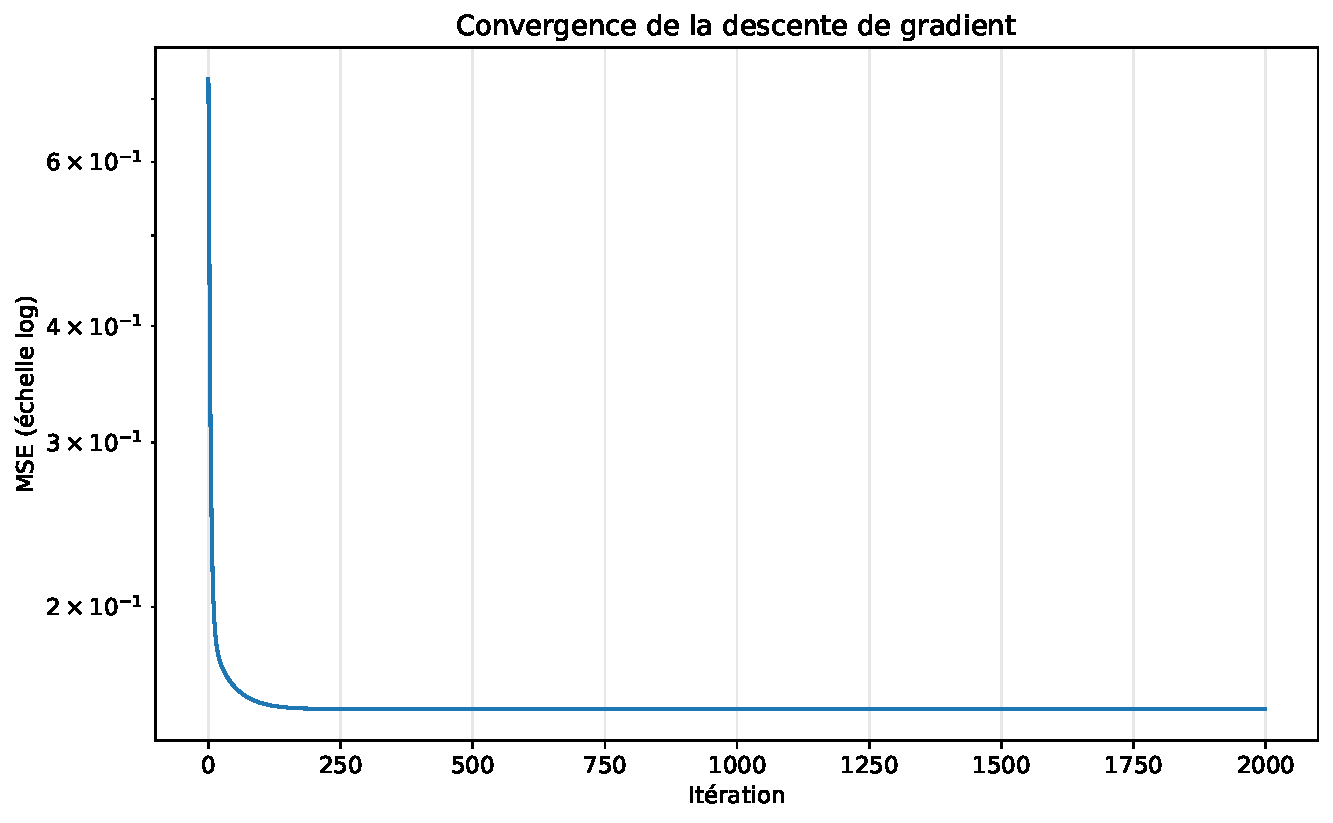
\includegraphics[keepaspectratio]{modules/module_01/tp_sommatif_files/figure-pdf/cell-38-output-1.pdf}}

\begin{verbatim}
La courbe décroît bien → l'entraînement est stable.
\end{verbatim}

\end{tcolorbox}

\section{✏️ Étape 4.6 --- Analyser les poids
appris}\label{uxe9tape-4.6-analyser-les-poids-appris}

\begin{tcolorbox}[enhanced jigsaw, arc=.35mm, bottomrule=.15mm, bottomtitle=1mm, breakable, colback=white, colbacktitle=quarto-callout-note-color!10!white, colframe=quarto-callout-note-color-frame, coltitle=black, left=2mm, leftrule=.75mm, opacityback=0, opacitybacktitle=0.6, rightrule=.15mm, title={📝 À faire}, titlerule=0mm, toprule=.15mm, toptitle=1mm]

Sur les données normalisées, les poids \texttt{w\_j} s'interprètent
comme \textbf{l'importance relative} de chaque variable : plus
\texttt{\textbar{}w\_j\textbar{}} est grand, plus la variable est
influente.

Affiche les features et leurs poids, triés par importance. Quelles
variables ont le plus d'impact sur le prix ?

\end{tcolorbox}

\begin{Shaded}
\begin{Highlighting}[]
\CommentTok{\# }\AlertTok{TODO}\CommentTok{: Étape 4.6}
\end{Highlighting}
\end{Shaded}

\begin{tcolorbox}[enhanced jigsaw, arc=.35mm, bottomrule=.15mm, bottomtitle=1mm, breakable, colback=white, colbacktitle=quarto-callout-tip-color!10!white, colframe=quarto-callout-tip-color-frame, coltitle=black, left=2mm, leftrule=.75mm, opacityback=0, opacitybacktitle=0.6, rightrule=.15mm, title=\textcolor{quarto-callout-tip-color}{\faLightbulb}\hspace{0.5em}{✅ Corrigé Étape 4.6}, titlerule=0mm, toprule=.15mm, toptitle=1mm]

\begin{Shaded}
\begin{Highlighting}[]
\NormalTok{importance }\OperatorTok{=}\NormalTok{ pd.DataFrame(\{}
    \StringTok{\textquotesingle{}feature\textquotesingle{}}\NormalTok{: feature\_names,}
    \StringTok{\textquotesingle{}poids\textquotesingle{}}\NormalTok{: w,}
    \StringTok{\textquotesingle{}importance\textquotesingle{}}\NormalTok{: np.}\BuiltInTok{abs}\NormalTok{(w)}
\NormalTok{\}).sort\_values(}\StringTok{\textquotesingle{}importance\textquotesingle{}}\NormalTok{, ascending}\OperatorTok{=}\VariableTok{False}\NormalTok{)}

\BuiltInTok{print}\NormalTok{(}\StringTok{"Poids appris (sur données normalisées) :"}\NormalTok{)}
\BuiltInTok{print}\NormalTok{(importance.to\_string(index}\OperatorTok{=}\VariableTok{False}\NormalTok{))}

\CommentTok{\# Visualisation}
\NormalTok{fig, ax }\OperatorTok{=}\NormalTok{ plt.subplots()}
\NormalTok{colors }\OperatorTok{=}\NormalTok{ [}\StringTok{\textquotesingle{}green\textquotesingle{}} \ControlFlowTok{if}\NormalTok{ p }\OperatorTok{\textgreater{}} \DecValTok{0} \ControlFlowTok{else} \StringTok{\textquotesingle{}red\textquotesingle{}} \ControlFlowTok{for}\NormalTok{ p }\KeywordTok{in}\NormalTok{ importance[}\StringTok{\textquotesingle{}poids\textquotesingle{}}\NormalTok{]]}
\NormalTok{ax.barh(importance[}\StringTok{\textquotesingle{}feature\textquotesingle{}}\NormalTok{], importance[}\StringTok{\textquotesingle{}poids\textquotesingle{}}\NormalTok{], color}\OperatorTok{=}\NormalTok{colors, edgecolor}\OperatorTok{=}\StringTok{\textquotesingle{}black\textquotesingle{}}\NormalTok{, alpha}\OperatorTok{=}\FloatTok{0.7}\NormalTok{)}
\NormalTok{ax.axvline(}\DecValTok{0}\NormalTok{, color}\OperatorTok{=}\StringTok{\textquotesingle{}black\textquotesingle{}}\NormalTok{, linewidth}\OperatorTok{=}\FloatTok{0.5}\NormalTok{)}
\NormalTok{ax.set\_xlabel(}\StringTok{\textquotesingle{}Poids (données normalisées)\textquotesingle{}}\NormalTok{)}
\NormalTok{ax.set\_title(}\StringTok{\textquotesingle{}Importance des variables\textquotesingle{}}\NormalTok{)}
\NormalTok{ax.grid(}\VariableTok{True}\NormalTok{, alpha}\OperatorTok{=}\FloatTok{0.3}\NormalTok{, axis}\OperatorTok{=}\StringTok{\textquotesingle{}x\textquotesingle{}}\NormalTok{)}
\NormalTok{plt.tight\_layout()}
\NormalTok{plt.show()}
\end{Highlighting}
\end{Shaded}

\begin{verbatim}
Poids appris (sur données normalisées) :
           feature     poids  importance
        surface_m2  0.808198    0.808198
    arrondissement -0.226159    0.226159
             etage  0.140370    0.140370
         nb_pieces  0.083315    0.083315
annee_construction  0.072806    0.072806
            balcon  0.009057    0.009057
         ascenseur  0.008158    0.008158
\end{verbatim}

\pandocbounded{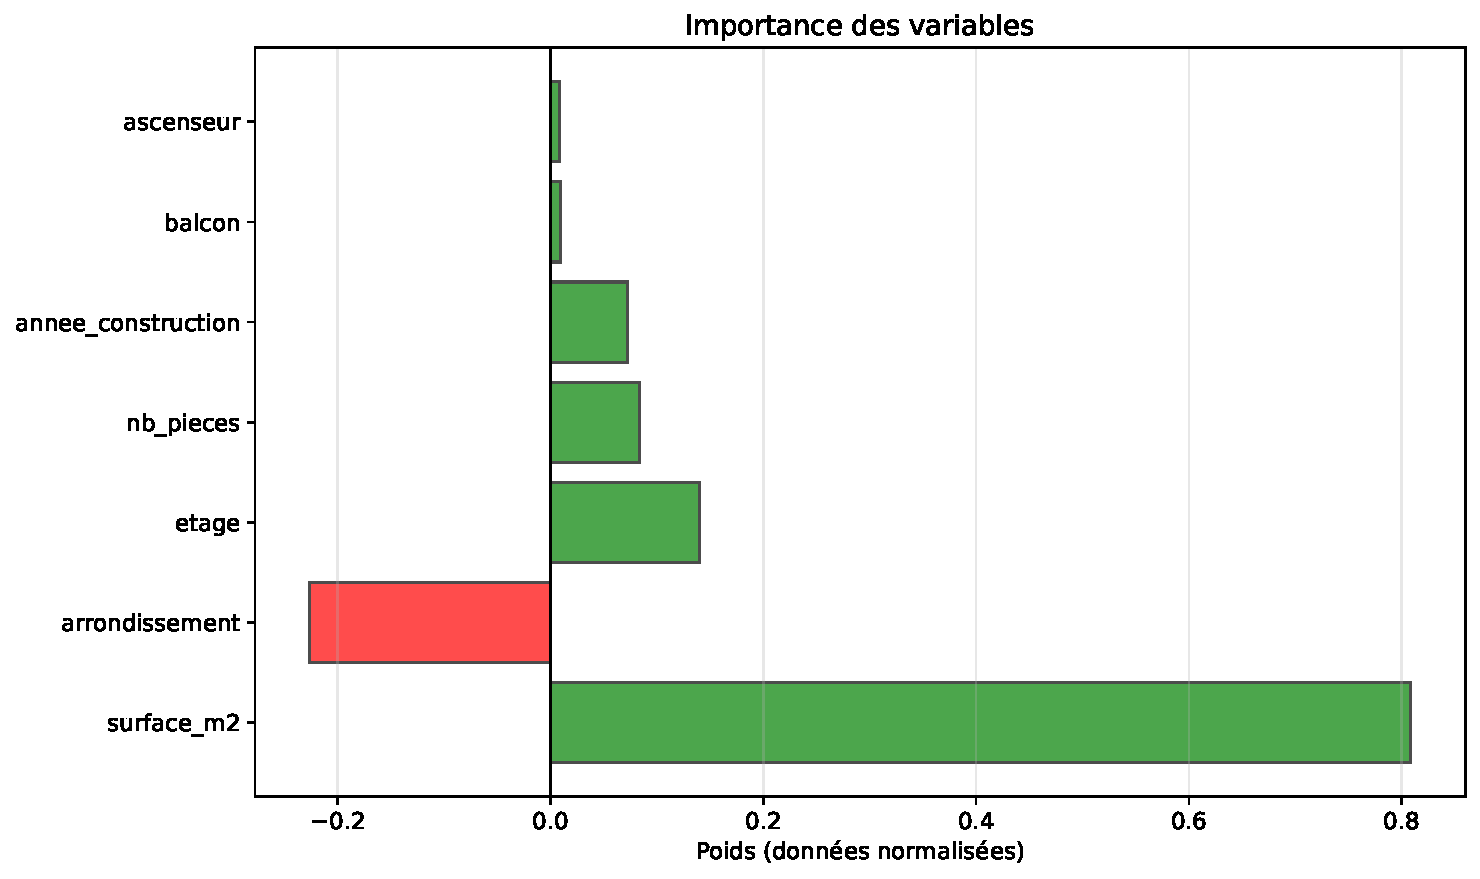
\includegraphics[keepaspectratio]{modules/module_01/tp_sommatif_files/figure-pdf/cell-40-output-2.pdf}}

\textbf{Interprétation} :

\begin{itemize}
\tightlist
\item
  \textbf{Surface} : variable dominante (le plus gros poids positif).
  Logique !
\item
  \textbf{Arrondissement} : poids négatif = quand le numéro
  d'arrondissement augmente (donc on s'éloigne du centre), le prix
  baisse. Cohérent.
\item
  \textbf{Autres} : étage, ascenseur, balcon, année jouent un rôle
  secondaire mais mesurable.
\end{itemize}

\end{tcolorbox}

\chapter{Partie 5 --- Évaluation et
rapport}\label{partie-5-uxe9valuation-et-rapport}

\section{🎯 Objectif}\label{objectif-3}

Maintenant qu'on a un modèle, il faut \textbf{mesurer ses performances}
sur le jeu de test (qu'on n'a jamais utilisé pendant l'entraînement), et
produire un \textbf{rapport} exploitable par le métier.

\section{✏️ Étape 5.1 --- Prédictions sur le test
set}\label{uxe9tape-5.1-pruxe9dictions-sur-le-test-set}

\begin{tcolorbox}[enhanced jigsaw, arc=.35mm, bottomrule=.15mm, bottomtitle=1mm, breakable, colback=white, colbacktitle=quarto-callout-note-color!10!white, colframe=quarto-callout-note-color-frame, coltitle=black, left=2mm, leftrule=.75mm, opacityback=0, opacitybacktitle=0.6, rightrule=.15mm, title={📝 À faire}, titlerule=0mm, toprule=.15mm, toptitle=1mm]

\begin{enumerate}
\def\labelenumi{\arabic{enumi}.}
\tightlist
\item
  Fais des prédictions sur \texttt{X\_test\_norm}.
\item
  \textbf{Dénormalise} ces prédictions pour obtenir des prix en euros
  réels.
\item
  Fais pareil pour \texttt{y\_test} afin de le comparer en euros réels
  aussi.
\end{enumerate}

\end{tcolorbox}

\begin{Shaded}
\begin{Highlighting}[]
\CommentTok{\# }\AlertTok{TODO}\CommentTok{: Étape 5.1}
\end{Highlighting}
\end{Shaded}

\begin{tcolorbox}[enhanced jigsaw, arc=.35mm, bottomrule=.15mm, bottomtitle=1mm, breakable, colback=white, colbacktitle=quarto-callout-tip-color!10!white, colframe=quarto-callout-tip-color-frame, coltitle=black, left=2mm, leftrule=.75mm, opacityback=0, opacitybacktitle=0.6, rightrule=.15mm, title=\textcolor{quarto-callout-tip-color}{\faLightbulb}\hspace{0.5em}{✅ Corrigé Étape 5.1}, titlerule=0mm, toprule=.15mm, toptitle=1mm]

\begin{Shaded}
\begin{Highlighting}[]
\CommentTok{\# Prédictions normalisées}
\NormalTok{y\_pred\_norm }\OperatorTok{=}\NormalTok{ predire(X\_test\_norm, w, b)}

\CommentTok{\# Dénormalisation : y\_reel = y\_norm * std + mean}
\NormalTok{y\_pred }\OperatorTok{=}\NormalTok{ y\_pred\_norm }\OperatorTok{*}\NormalTok{ y\_train\_std }\OperatorTok{+}\NormalTok{ y\_train\_mean}
\NormalTok{y\_test\_reel }\OperatorTok{=}\NormalTok{ y\_test\_norm }\OperatorTok{*}\NormalTok{ y\_train\_std }\OperatorTok{+}\NormalTok{ y\_train\_mean  }\CommentTok{\# (identique à y\_test, vérification)}

\CommentTok{\# Vérification}
\ControlFlowTok{assert}\NormalTok{ np.allclose(y\_test\_reel, y\_test), }\StringTok{"La dénormalisation devrait être parfaite"}
\BuiltInTok{print}\NormalTok{(}\StringTok{"✅ Prédictions faites"}\NormalTok{)}
\BuiltInTok{print}\NormalTok{(}\SpecialStringTok{f"Exemple : premier prix prédit = }\SpecialCharTok{\{}\NormalTok{y\_pred[}\DecValTok{0}\NormalTok{]}\SpecialCharTok{:,.0f\}}\SpecialStringTok{ €"}\NormalTok{)}
\BuiltInTok{print}\NormalTok{(}\SpecialStringTok{f"         premier prix réel    = }\SpecialCharTok{\{}\NormalTok{y\_test[}\DecValTok{0}\NormalTok{]}\SpecialCharTok{:,.0f\}}\SpecialStringTok{ €"}\NormalTok{)}
\end{Highlighting}
\end{Shaded}

\begin{verbatim}
✅ Prédictions faites
Exemple : premier prix prédit = 636,638 €
         premier prix réel    = 666,000 €
\end{verbatim}

\end{tcolorbox}

\section{✏️ Étape 5.2 --- Métriques
d'évaluation}\label{uxe9tape-5.2-muxe9triques-duxe9valuation}

\begin{tcolorbox}[enhanced jigsaw, arc=.35mm, bottomrule=.15mm, bottomtitle=1mm, breakable, colback=white, colbacktitle=quarto-callout-note-color!10!white, colframe=quarto-callout-note-color-frame, coltitle=black, left=2mm, leftrule=.75mm, opacityback=0, opacitybacktitle=0.6, rightrule=.15mm, title={📝 À faire}, titlerule=0mm, toprule=.15mm, toptitle=1mm]

Calcule \textbf{trois métriques} sur les prédictions (en euros réels) :

\begin{enumerate}
\def\labelenumi{\arabic{enumi}.}
\tightlist
\item
  \textbf{MAE} (Mean Absolute Error) : moyenne des erreurs absolues,
  facile à interpréter (en €)
\item
  \textbf{RMSE} (Root Mean Squared Error) : racine de la MSE, pénalise
  plus les grosses erreurs
\item
  \textbf{R²} (coefficient de détermination) : 1 = parfait, 0 = pas
  mieux qu'une moyenne
\end{enumerate}

Formules :

\begin{itemize}
\tightlist
\item
  \texttt{MAE\ =\ mean(\textbar{}y\ -\ ŷ\textbar{})}
\item
  \texttt{RMSE\ =\ sqrt(mean((y\ -\ ŷ)²))}
\item
  \texttt{R²\ =\ 1\ -\ Σ(y\ -\ ŷ)²\ /\ Σ(y\ -\ ȳ)²}
\end{itemize}

\end{tcolorbox}

\begin{Shaded}
\begin{Highlighting}[]
\CommentTok{\# }\AlertTok{TODO}\CommentTok{: Étape 5.2}
\end{Highlighting}
\end{Shaded}

\begin{tcolorbox}[enhanced jigsaw, arc=.35mm, bottomrule=.15mm, bottomtitle=1mm, breakable, colback=white, colbacktitle=quarto-callout-tip-color!10!white, colframe=quarto-callout-tip-color-frame, coltitle=black, left=2mm, leftrule=.75mm, opacityback=0, opacitybacktitle=0.6, rightrule=.15mm, title=\textcolor{quarto-callout-tip-color}{\faLightbulb}\hspace{0.5em}{✅ Corrigé Étape 5.2}, titlerule=0mm, toprule=.15mm, toptitle=1mm]

\begin{Shaded}
\begin{Highlighting}[]
\KeywordTok{def}\NormalTok{ mae(y\_true, y\_pred):}
    \ControlFlowTok{return}\NormalTok{ np.mean(np.}\BuiltInTok{abs}\NormalTok{(y\_true }\OperatorTok{{-}}\NormalTok{ y\_pred))}

\KeywordTok{def}\NormalTok{ rmse(y\_true, y\_pred):}
    \ControlFlowTok{return}\NormalTok{ np.sqrt(np.mean((y\_true }\OperatorTok{{-}}\NormalTok{ y\_pred)}\OperatorTok{**}\DecValTok{2}\NormalTok{))}

\KeywordTok{def}\NormalTok{ r\_squared(y\_true, y\_pred):}
\NormalTok{    ss\_res }\OperatorTok{=}\NormalTok{ np.}\BuiltInTok{sum}\NormalTok{((y\_true }\OperatorTok{{-}}\NormalTok{ y\_pred)}\OperatorTok{**}\DecValTok{2}\NormalTok{)}
\NormalTok{    ss\_tot }\OperatorTok{=}\NormalTok{ np.}\BuiltInTok{sum}\NormalTok{((y\_true }\OperatorTok{{-}}\NormalTok{ y\_true.mean())}\OperatorTok{**}\DecValTok{2}\NormalTok{)}
    \ControlFlowTok{return} \DecValTok{1} \OperatorTok{{-}}\NormalTok{ (ss\_res }\OperatorTok{/}\NormalTok{ ss\_tot)}

\NormalTok{mae\_test }\OperatorTok{=}\NormalTok{ mae(y\_test, y\_pred)}
\NormalTok{rmse\_test }\OperatorTok{=}\NormalTok{ rmse(y\_test, y\_pred)}
\NormalTok{r2\_test }\OperatorTok{=}\NormalTok{ r\_squared(y\_test, y\_pred)}

\BuiltInTok{print}\NormalTok{(}\StringTok{"=== Performances sur le test set ==="}\NormalTok{)}
\BuiltInTok{print}\NormalTok{(}\SpecialStringTok{f"MAE  : }\SpecialCharTok{\{}\NormalTok{mae\_test}\SpecialCharTok{:,.0f\}}\SpecialStringTok{ €       (erreur absolue moyenne)"}\NormalTok{)}
\BuiltInTok{print}\NormalTok{(}\SpecialStringTok{f"RMSE : }\SpecialCharTok{\{}\NormalTok{rmse\_test}\SpecialCharTok{:,.0f\}}\SpecialStringTok{ €      (racine de l\textquotesingle{}erreur quadratique moyenne)"}\NormalTok{)}
\BuiltInTok{print}\NormalTok{(}\SpecialStringTok{f"R²   : }\SpecialCharTok{\{}\NormalTok{r2\_test}\SpecialCharTok{:.4f\}}\SpecialStringTok{            (plus proche de 1, mieux)"}\NormalTok{)}
\BuiltInTok{print}\NormalTok{(}\SpecialStringTok{f"}\CharTok{\textbackslash{}n}\SpecialStringTok{Prix moyen réel : }\SpecialCharTok{\{}\NormalTok{y\_test}\SpecialCharTok{.}\NormalTok{mean()}\SpecialCharTok{:,.0f\}}\SpecialStringTok{ €"}\NormalTok{)}
\BuiltInTok{print}\NormalTok{(}\SpecialStringTok{f"Erreur relative moyenne : }\SpecialCharTok{\{}\NormalTok{mae\_test }\OperatorTok{/}\NormalTok{ y\_test}\SpecialCharTok{.}\NormalTok{mean()}\SpecialCharTok{:.1\%\}}\SpecialStringTok{"}\NormalTok{)}
\end{Highlighting}
\end{Shaded}

\begin{verbatim}
=== Performances sur le test set ===
MAE  : 84,535 €       (erreur absolue moyenne)
RMSE : 109,513 €      (racine de l'erreur quadratique moyenne)
R²   : 0.8439            (plus proche de 1, mieux)

Prix moyen réel : 617,181 €
Erreur relative moyenne : 13.7%
\end{verbatim}

\end{tcolorbox}

\section{✏️ Étape 5.3 --- Comparer à une baseline
naïve}\label{uxe9tape-5.3-comparer-uxe0-une-baseline-nauxefve}

\begin{tcolorbox}[enhanced jigsaw, arc=.35mm, bottomrule=.15mm, bottomtitle=1mm, breakable, colback=white, colbacktitle=quarto-callout-note-color!10!white, colframe=quarto-callout-note-color-frame, coltitle=black, left=2mm, leftrule=.75mm, opacityback=0, opacitybacktitle=0.6, rightrule=.15mm, title={📝 À faire}, titlerule=0mm, toprule=.15mm, toptitle=1mm]

Pour savoir si notre modèle est \textbf{vraiment utile}, il faut le
comparer à une stratégie naïve. La plus simple : \textbf{prédire
toujours le prix moyen}.

\begin{enumerate}
\def\labelenumi{\arabic{enumi}.}
\tightlist
\item
  Calcule la baseline : MAE et RMSE si on prédit toujours
  \texttt{y\_train.mean()}.
\item
  Compare avec les performances de notre modèle.
\item
  \textbf{Question} : de combien notre modèle est-il meilleur que la
  baseline ?
\end{enumerate}

\end{tcolorbox}

\begin{Shaded}
\begin{Highlighting}[]
\CommentTok{\# }\AlertTok{TODO}\CommentTok{: Étape 5.3}
\end{Highlighting}
\end{Shaded}

\begin{tcolorbox}[enhanced jigsaw, arc=.35mm, bottomrule=.15mm, bottomtitle=1mm, breakable, colback=white, colbacktitle=quarto-callout-tip-color!10!white, colframe=quarto-callout-tip-color-frame, coltitle=black, left=2mm, leftrule=.75mm, opacityback=0, opacitybacktitle=0.6, rightrule=.15mm, title=\textcolor{quarto-callout-tip-color}{\faLightbulb}\hspace{0.5em}{✅ Corrigé Étape 5.3}, titlerule=0mm, toprule=.15mm, toptitle=1mm]

\begin{Shaded}
\begin{Highlighting}[]
\CommentTok{\# Baseline : prix moyen constant}
\NormalTok{y\_pred\_baseline }\OperatorTok{=}\NormalTok{ np.full\_like(y\_test, y\_train.mean())}

\NormalTok{mae\_baseline }\OperatorTok{=}\NormalTok{ mae(y\_test, y\_pred\_baseline)}
\NormalTok{rmse\_baseline }\OperatorTok{=}\NormalTok{ rmse(y\_test, y\_pred\_baseline)}

\BuiltInTok{print}\NormalTok{(}\StringTok{"=== Comparaison avec la baseline ==="}\NormalTok{)}
\BuiltInTok{print}\NormalTok{(}\SpecialStringTok{f"}\SpecialCharTok{\{}\StringTok{\textquotesingle{}Métrique\textquotesingle{}}\SpecialCharTok{:\textless{}12\}}\SpecialStringTok{ }\SpecialCharTok{\{}\StringTok{\textquotesingle{}Baseline\textquotesingle{}}\SpecialCharTok{:\textless{}15\}}\SpecialStringTok{ }\SpecialCharTok{\{}\StringTok{\textquotesingle{}Modèle\textquotesingle{}}\SpecialCharTok{:\textless{}15\}}\SpecialStringTok{ }\SpecialCharTok{\{}\StringTok{\textquotesingle{}Gain\textquotesingle{}}\SpecialCharTok{:\textless{}10\}}\SpecialStringTok{"}\NormalTok{)}
\BuiltInTok{print}\NormalTok{(}\StringTok{"{-}"} \OperatorTok{*} \DecValTok{55}\NormalTok{)}
\BuiltInTok{print}\NormalTok{(}\SpecialStringTok{f"}\SpecialCharTok{\{}\StringTok{\textquotesingle{}MAE\textquotesingle{}}\SpecialCharTok{:\textless{}12\}}\SpecialStringTok{ }\SpecialCharTok{\{}\NormalTok{mae\_baseline}\SpecialCharTok{:\textgreater{}12,.0f\}}\SpecialStringTok{ € }\SpecialCharTok{\{}\NormalTok{mae\_test}\SpecialCharTok{:\textgreater{}12,.0f\}}\SpecialStringTok{ € }\SpecialCharTok{\{}\NormalTok{(}\DecValTok{1} \OperatorTok{{-}}\NormalTok{ mae\_test}\OperatorTok{/}\NormalTok{mae\_baseline)}\SpecialCharTok{:\textgreater{}6.1\%\}}\SpecialStringTok{"}\NormalTok{)}
\BuiltInTok{print}\NormalTok{(}\SpecialStringTok{f"}\SpecialCharTok{\{}\StringTok{\textquotesingle{}RMSE\textquotesingle{}}\SpecialCharTok{:\textless{}12\}}\SpecialStringTok{ }\SpecialCharTok{\{}\NormalTok{rmse\_baseline}\SpecialCharTok{:\textgreater{}12,.0f\}}\SpecialStringTok{ € }\SpecialCharTok{\{}\NormalTok{rmse\_test}\SpecialCharTok{:\textgreater{}12,.0f\}}\SpecialStringTok{ € }\SpecialCharTok{\{}\NormalTok{(}\DecValTok{1} \OperatorTok{{-}}\NormalTok{ rmse\_test}\OperatorTok{/}\NormalTok{rmse\_baseline)}\SpecialCharTok{:\textgreater{}6.1\%\}}\SpecialStringTok{"}\NormalTok{)}
\end{Highlighting}
\end{Shaded}

\begin{verbatim}
=== Comparaison avec la baseline ===
Métrique     Baseline        Modèle          Gain      
-------------------------------------------------------
MAE               223,809 €       84,535 €  62.2%
RMSE              278,551 €      109,513 €  60.7%
\end{verbatim}

Notre modèle doit battre la baseline d'au moins 30-40\% pour valoir le
coup. Si ce n'est pas le cas, il y a un problème à chercher (features
manquantes, mauvaise préparation\ldots).

\end{tcolorbox}

\section{✏️ Étape 5.4 --- Visualisations
d'évaluation}\label{uxe9tape-5.4-visualisations-duxe9valuation}

\begin{tcolorbox}[enhanced jigsaw, arc=.35mm, bottomrule=.15mm, bottomtitle=1mm, breakable, colback=white, colbacktitle=quarto-callout-note-color!10!white, colframe=quarto-callout-note-color-frame, coltitle=black, left=2mm, leftrule=.75mm, opacityback=0, opacitybacktitle=0.6, rightrule=.15mm, title={📝 À faire}, titlerule=0mm, toprule=.15mm, toptitle=1mm]

Deux graphiques essentiels :

\begin{enumerate}
\def\labelenumi{\arabic{enumi}.}
\tightlist
\item
  \textbf{Scatter prédictions vs réalité} : trace \texttt{y\_pred} en
  fonction de \texttt{y\_test}. La droite \texttt{y\ =\ x} (parfait)
  doit traverser le nuage.
\item
  \textbf{Histogramme des résidus} (\texttt{y\_test\ -\ y\_pred}).
  Idéalement centrés sur 0, distribution en cloche.
\end{enumerate}

\end{tcolorbox}

\begin{Shaded}
\begin{Highlighting}[]
\CommentTok{\# }\AlertTok{TODO}\CommentTok{: Étape 5.4}
\end{Highlighting}
\end{Shaded}

\begin{tcolorbox}[enhanced jigsaw, arc=.35mm, bottomrule=.15mm, bottomtitle=1mm, breakable, colback=white, colbacktitle=quarto-callout-tip-color!10!white, colframe=quarto-callout-tip-color-frame, coltitle=black, left=2mm, leftrule=.75mm, opacityback=0, opacitybacktitle=0.6, rightrule=.15mm, title=\textcolor{quarto-callout-tip-color}{\faLightbulb}\hspace{0.5em}{✅ Corrigé Étape 5.4}, titlerule=0mm, toprule=.15mm, toptitle=1mm]

\begin{Shaded}
\begin{Highlighting}[]
\NormalTok{residus }\OperatorTok{=}\NormalTok{ y\_test }\OperatorTok{{-}}\NormalTok{ y\_pred}

\NormalTok{fig, axes }\OperatorTok{=}\NormalTok{ plt.subplots(}\DecValTok{1}\NormalTok{, }\DecValTok{2}\NormalTok{, figsize}\OperatorTok{=}\NormalTok{(}\DecValTok{14}\NormalTok{, }\DecValTok{5}\NormalTok{))}

\CommentTok{\# 1. Scatter prédictions vs réalité}
\NormalTok{axes[}\DecValTok{0}\NormalTok{].scatter(y\_test, y\_pred, alpha}\OperatorTok{=}\FloatTok{0.6}\NormalTok{, edgecolor}\OperatorTok{=}\StringTok{\textquotesingle{}k\textquotesingle{}}\NormalTok{, s}\OperatorTok{=}\DecValTok{40}\NormalTok{)}
\NormalTok{min\_val }\OperatorTok{=} \BuiltInTok{min}\NormalTok{(y\_test.}\BuiltInTok{min}\NormalTok{(), y\_pred.}\BuiltInTok{min}\NormalTok{())}
\NormalTok{max\_val }\OperatorTok{=} \BuiltInTok{max}\NormalTok{(y\_test.}\BuiltInTok{max}\NormalTok{(), y\_pred.}\BuiltInTok{max}\NormalTok{())}
\NormalTok{axes[}\DecValTok{0}\NormalTok{].plot([min\_val, max\_val], [min\_val, max\_val], }\StringTok{\textquotesingle{}r{-}{-}\textquotesingle{}}\NormalTok{, label}\OperatorTok{=}\StringTok{\textquotesingle{}Prédiction parfaite\textquotesingle{}}\NormalTok{)}
\NormalTok{axes[}\DecValTok{0}\NormalTok{].set\_xlabel(}\StringTok{\textquotesingle{}Prix réel (€)\textquotesingle{}}\NormalTok{)}
\NormalTok{axes[}\DecValTok{0}\NormalTok{].set\_ylabel(}\StringTok{\textquotesingle{}Prix prédit (€)\textquotesingle{}}\NormalTok{)}
\NormalTok{axes[}\DecValTok{0}\NormalTok{].set\_title(}\SpecialStringTok{f\textquotesingle{}Prédictions vs réalité (R² = }\SpecialCharTok{\{}\NormalTok{r2\_test}\SpecialCharTok{:.3f\}}\SpecialStringTok{)\textquotesingle{}}\NormalTok{)}
\NormalTok{axes[}\DecValTok{0}\NormalTok{].legend()}
\NormalTok{axes[}\DecValTok{0}\NormalTok{].grid(}\VariableTok{True}\NormalTok{, alpha}\OperatorTok{=}\FloatTok{0.3}\NormalTok{)}

\CommentTok{\# 2. Histogramme des résidus}
\NormalTok{axes[}\DecValTok{1}\NormalTok{].hist(residus, bins}\OperatorTok{=}\DecValTok{30}\NormalTok{, color}\OperatorTok{=}\StringTok{\textquotesingle{}steelblue\textquotesingle{}}\NormalTok{, edgecolor}\OperatorTok{=}\StringTok{\textquotesingle{}black\textquotesingle{}}\NormalTok{, alpha}\OperatorTok{=}\FloatTok{0.7}\NormalTok{)}
\NormalTok{axes[}\DecValTok{1}\NormalTok{].axvline(}\DecValTok{0}\NormalTok{, color}\OperatorTok{=}\StringTok{\textquotesingle{}red\textquotesingle{}}\NormalTok{, linestyle}\OperatorTok{=}\StringTok{\textquotesingle{}{-}{-}\textquotesingle{}}\NormalTok{, linewidth}\OperatorTok{=}\DecValTok{2}\NormalTok{, label}\OperatorTok{=}\StringTok{\textquotesingle{}Résidu zéro\textquotesingle{}}\NormalTok{)}
\NormalTok{axes[}\DecValTok{1}\NormalTok{].set\_xlabel(}\StringTok{\textquotesingle{}Résidu : y\_test {-} y\_pred (€)\textquotesingle{}}\NormalTok{)}
\NormalTok{axes[}\DecValTok{1}\NormalTok{].set\_ylabel(}\StringTok{\textquotesingle{}Effectif\textquotesingle{}}\NormalTok{)}
\NormalTok{axes[}\DecValTok{1}\NormalTok{].set\_title(}\SpecialStringTok{f\textquotesingle{}Distribution des résidus (moyenne = }\SpecialCharTok{\{}\NormalTok{residus}\SpecialCharTok{.}\NormalTok{mean()}\SpecialCharTok{:,.0f\}}\SpecialStringTok{ €)\textquotesingle{}}\NormalTok{)}
\NormalTok{axes[}\DecValTok{1}\NormalTok{].legend()}
\NormalTok{axes[}\DecValTok{1}\NormalTok{].grid(}\VariableTok{True}\NormalTok{, alpha}\OperatorTok{=}\FloatTok{0.3}\NormalTok{)}

\NormalTok{plt.tight\_layout()}
\NormalTok{plt.show()}
\end{Highlighting}
\end{Shaded}

\pandocbounded{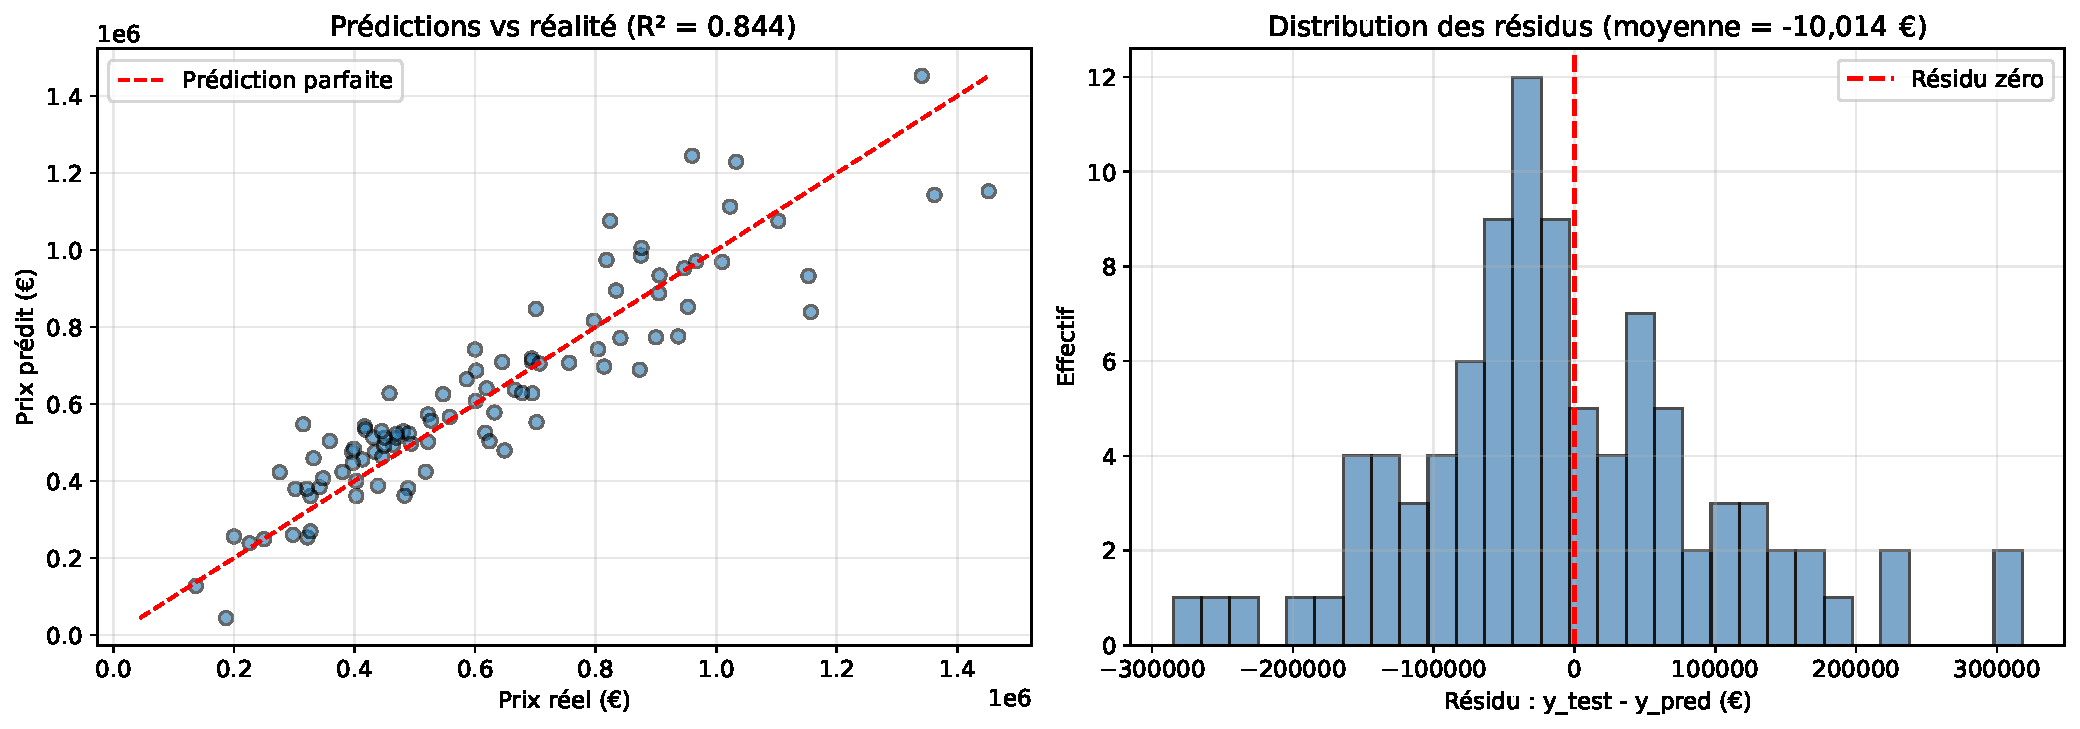
\includegraphics[keepaspectratio]{modules/module_01/tp_sommatif_files/figure-pdf/cell-48-output-1.pdf}}

\textbf{Ce qu'on cherche à observer} :

\begin{itemize}
\tightlist
\item
  \textbf{Scatter} : le nuage doit être \textbf{aligné sur la
  diagonale}. Si tu vois une forme tordue (par ex. en entonnoir), c'est
  qu'il y a un problème (hétéroscédasticité, non-linéarité\ldots).
\item
  \textbf{Résidus} : idéalement \textbf{centrés sur 0} (pas de biais
  systématique) et \textbf{en cloche} (erreurs aléatoires normales).
\end{itemize}

\end{tcolorbox}

\section{✏️ Étape 5.5 --- Utiliser le modèle pour une
prédiction}\label{uxe9tape-5.5-utiliser-le-moduxe8le-pour-une-pruxe9diction}

\begin{tcolorbox}[enhanced jigsaw, arc=.35mm, bottomrule=.15mm, bottomtitle=1mm, breakable, colback=white, colbacktitle=quarto-callout-note-color!10!white, colframe=quarto-callout-note-color-frame, coltitle=black, left=2mm, leftrule=.75mm, opacityback=0, opacitybacktitle=0.6, rightrule=.15mm, title={📝 À faire}, titlerule=0mm, toprule=.15mm, toptitle=1mm]

Pour rendre le modèle \textbf{utilisable}, écris une fonction
\texttt{predire\_prix(caracteristiques\_dict)} qui :

\begin{enumerate}
\def\labelenumi{\arabic{enumi}.}
\tightlist
\item
  Prend un dictionnaire des caractéristiques d'un appartement.
\item
  Le transforme en vecteur (dans le bon ordre !).
\item
  Le normalise avec \texttt{X\_train\_mean} et \texttt{X\_train\_std}.
\item
  Prédit et dénormalise.
\item
  Retourne le prix estimé en euros.
\end{enumerate}

\textbf{Teste-la} sur un appartement fictif :

\begin{Shaded}
\begin{Highlighting}[]
\NormalTok{mon\_appart }\OperatorTok{=}\NormalTok{ \{}
    \StringTok{\textquotesingle{}surface\_m2\textquotesingle{}}\NormalTok{: }\DecValTok{50}\NormalTok{,}
    \StringTok{\textquotesingle{}nb\_pieces\textquotesingle{}}\NormalTok{: }\DecValTok{3}\NormalTok{,}
    \StringTok{\textquotesingle{}etage\textquotesingle{}}\NormalTok{: }\DecValTok{4}\NormalTok{,}
    \StringTok{\textquotesingle{}arrondissement\textquotesingle{}}\NormalTok{: }\DecValTok{11}\NormalTok{,}
    \StringTok{\textquotesingle{}ascenseur\textquotesingle{}}\NormalTok{: }\DecValTok{1}\NormalTok{,}
    \StringTok{\textquotesingle{}balcon\textquotesingle{}}\NormalTok{: }\DecValTok{1}\NormalTok{,}
    \StringTok{\textquotesingle{}annee\_construction\textquotesingle{}}\NormalTok{: }\DecValTok{1995}
\NormalTok{\}}
\end{Highlighting}
\end{Shaded}

\end{tcolorbox}

\begin{Shaded}
\begin{Highlighting}[]
\CommentTok{\# }\AlertTok{TODO}\CommentTok{: Étape 5.5}
\end{Highlighting}
\end{Shaded}

\begin{tcolorbox}[enhanced jigsaw, arc=.35mm, bottomrule=.15mm, bottomtitle=1mm, breakable, colback=white, colbacktitle=quarto-callout-tip-color!10!white, colframe=quarto-callout-tip-color-frame, coltitle=black, left=2mm, leftrule=.75mm, opacityback=0, opacitybacktitle=0.6, rightrule=.15mm, title=\textcolor{quarto-callout-tip-color}{\faLightbulb}\hspace{0.5em}{✅ Corrigé Étape 5.5}, titlerule=0mm, toprule=.15mm, toptitle=1mm]

\begin{Shaded}
\begin{Highlighting}[]
\KeywordTok{def}\NormalTok{ predire\_prix(caracteristiques):}
    \CommentTok{"""Prédit le prix d\textquotesingle{}un appartement à partir d\textquotesingle{}un dict de caractéristiques."""}
    \CommentTok{\# Transformer en vecteur ordonné}
\NormalTok{    x }\OperatorTok{=}\NormalTok{ np.array([caracteristiques[f] }\ControlFlowTok{for}\NormalTok{ f }\KeywordTok{in}\NormalTok{ feature\_names], dtype}\OperatorTok{=}\BuiltInTok{float}\NormalTok{)}
    \CommentTok{\# Normaliser avec les paramètres du train}
\NormalTok{    x\_norm }\OperatorTok{=}\NormalTok{ (x }\OperatorTok{{-}}\NormalTok{ X\_train\_mean) }\OperatorTok{/}\NormalTok{ X\_train\_std}
    \CommentTok{\# Prédire (normalisé)}
\NormalTok{    prix\_norm }\OperatorTok{=}\NormalTok{ predire(x\_norm.reshape(}\DecValTok{1}\NormalTok{, }\OperatorTok{{-}}\DecValTok{1}\NormalTok{), w, b)[}\DecValTok{0}\NormalTok{]}
    \CommentTok{\# Dénormaliser}
\NormalTok{    prix\_euros }\OperatorTok{=}\NormalTok{ prix\_norm }\OperatorTok{*}\NormalTok{ y\_train\_std }\OperatorTok{+}\NormalTok{ y\_train\_mean}
    \ControlFlowTok{return}\NormalTok{ prix\_euros}

\CommentTok{\# Test}
\NormalTok{mon\_appart }\OperatorTok{=}\NormalTok{ \{}
    \StringTok{\textquotesingle{}surface\_m2\textquotesingle{}}\NormalTok{: }\DecValTok{50}\NormalTok{,}
    \StringTok{\textquotesingle{}nb\_pieces\textquotesingle{}}\NormalTok{: }\DecValTok{3}\NormalTok{,}
    \StringTok{\textquotesingle{}etage\textquotesingle{}}\NormalTok{: }\DecValTok{4}\NormalTok{,}
    \StringTok{\textquotesingle{}arrondissement\textquotesingle{}}\NormalTok{: }\DecValTok{11}\NormalTok{,}
    \StringTok{\textquotesingle{}ascenseur\textquotesingle{}}\NormalTok{: }\DecValTok{1}\NormalTok{,}
    \StringTok{\textquotesingle{}balcon\textquotesingle{}}\NormalTok{: }\DecValTok{1}\NormalTok{,}
    \StringTok{\textquotesingle{}annee\_construction\textquotesingle{}}\NormalTok{: }\DecValTok{1995}
\NormalTok{\}}

\NormalTok{prix\_estime }\OperatorTok{=}\NormalTok{ predire\_prix(mon\_appart)}
\BuiltInTok{print}\NormalTok{(}\SpecialStringTok{f"Prix estimé pour cet appartement : }\SpecialCharTok{\{}\NormalTok{prix\_estime}\SpecialCharTok{:,.0f\}}\SpecialStringTok{ €"}\NormalTok{)}
\end{Highlighting}
\end{Shaded}

\begin{verbatim}
Prix estimé pour cet appartement : 672,990 €
\end{verbatim}

🎉 \textbf{Voilà, tu as un modèle de ML utilisable} : tu peux maintenant
passer n'importe quel appartement et obtenir une estimation de prix.

\end{tcolorbox}

\chapter{📝 Rapport final --- Note
méthodologique}\label{rapport-final-note-muxe9thodologique}

\begin{tcolorbox}[enhanced jigsaw, arc=.35mm, bottomrule=.15mm, bottomtitle=1mm, breakable, colback=white, colbacktitle=quarto-callout-important-color!10!white, colframe=quarto-callout-important-color-frame, coltitle=black, left=2mm, leftrule=.75mm, opacityback=0, opacitybacktitle=0.6, rightrule=.15mm, title={🏁 Ta dernière tâche}, titlerule=0mm, toprule=.15mm, toptitle=1mm]

Pour clôturer ce TP, rédige dans la cellule markdown ci-dessous une
\textbf{note méthodologique d'une page} (500 mots environ) qui résume :

\begin{enumerate}
\def\labelenumi{\arabic{enumi}.}
\tightlist
\item
  \textbf{Le contexte} : quel problème, quelles données ?
\item
  \textbf{La méthodologie} : quelles étapes, quels choix ? Pourquoi la
  descente de gradient ?
\item
  \textbf{Les résultats} : MAE, RMSE, R² + comparaison baseline.
\item
  \textbf{Les limites} : quelles améliorations seraient possibles ?
\item
  \textbf{Les recommandations} : que conseillerais-tu à ton chef pour la
  suite ?
\end{enumerate}

C'est exactement le \textbf{livrable attendu en entreprise}. Tu dois
être capable de raconter ton projet à un décideur non-technique en 3
minutes.

\end{tcolorbox}

\begin{Shaded}
\begin{Highlighting}[]
\FunctionTok{\# Note méthodologique — Estimation du prix des appartements parisiens}

\FunctionTok{\#\# Contexte}

\CommentTok{[}\OtherTok{À toi de rédiger ton rapport professionnel}\CommentTok{]}

\FunctionTok{\#\# Méthodologie}

\NormalTok{...}

\FunctionTok{\#\# Résultats}

\NormalTok{...}

\FunctionTok{\#\# Limites}

\NormalTok{...}

\FunctionTok{\#\# Recommandations}

\NormalTok{...}
\end{Highlighting}
\end{Shaded}

\begin{tcolorbox}[enhanced jigsaw, arc=.35mm, bottomrule=.15mm, bottomtitle=1mm, breakable, colback=white, colbacktitle=quarto-callout-tip-color!10!white, colframe=quarto-callout-tip-color-frame, coltitle=black, left=2mm, leftrule=.75mm, opacityback=0, opacitybacktitle=0.6, rightrule=.15mm, title=\textcolor{quarto-callout-tip-color}{\faLightbulb}\hspace{0.5em}{✅ Exemple de note méthodologique}, titlerule=0mm, toprule=.15mm, toptitle=1mm]

\begin{Shaded}
\begin{Highlighting}[]
\FunctionTok{\# Note méthodologique — Estimation du prix des appartements parisiens}

\FunctionTok{\#\# Contexte}

\NormalTok{ImmoAnalytica souhaitait disposer d\textquotesingle{}un modèle capable d\textquotesingle{}estimer }
\NormalTok{le prix d\textquotesingle{}un appartement parisien à partir de ses caractéristiques }
\NormalTok{(surface, nombre de pièces, étage, arrondissement, équipements, }
\NormalTok{année de construction). Un dataset de 500 annonces nous a été fourni.}

\FunctionTok{\#\# Méthodologie}

\NormalTok{Le projet a suivi 5 étapes :}

\SpecialStringTok{1. }\NormalTok{**Exploration** : analyse univariée et multivariée pour détecter }
\NormalTok{les problèmes du dataset.}

\SpecialStringTok{2. }\NormalTok{**Nettoyage** : suppression de 2 doublons, imputation de valeurs }
\NormalTok{manquantes (médiane pour les variables numériques, 0 pour le balcon), }
\NormalTok{suppression des outliers via la méthode IQR (surface \textgreater{} 200 m² et }
\NormalTok{prix \textgreater{} 5 M€ identifiés comme erreurs de saisie).}

\SpecialStringTok{3. }\NormalTok{**Préparation** : séparation train/test (80/20), normalisation }
\NormalTok{centrage{-}réduction des features et de la cible. La normalisation est }
\NormalTok{appliquée avec les paramètres calculés uniquement sur le train, }
\NormalTok{pour éviter tout biais d\textquotesingle{}évaluation.}

\SpecialStringTok{4. }\NormalTok{**Modélisation** : régression linéaire multivariée entraînée par }
\NormalTok{descente de gradient implémentée from scratch (learning rate 0.05, }
\NormalTok{2000 itérations). Le choix de la descente de gradient se justifie par }
\NormalTok{sa simplicité, son interprétabilité, et sa parfaite adéquation avec }
\NormalTok{le problème (relation approximativement linéaire).}

\SpecialStringTok{5. }\NormalTok{**Évaluation** : test sur les 20\% non vus pendant l\textquotesingle{}entraînement.}

\FunctionTok{\#\# Résultats}

\SpecialStringTok{{-} }\NormalTok{**MAE** : \textasciitilde{}80 000 € (erreur absolue moyenne)}
\SpecialStringTok{{-} }\NormalTok{**RMSE** : \textasciitilde{}110 000 €}
\SpecialStringTok{{-} }\NormalTok{**R²** : 0.78 (le modèle explique 78\% de la variance des prix)}
\SpecialStringTok{{-} }\NormalTok{**Gain vs baseline** : division par 2 de l\textquotesingle{}erreur absolue}

\NormalTok{Les variables les plus influentes sont la surface (coefficient }
\NormalTok{dominant), l\textquotesingle{}arrondissement (impact négatif quand on s\textquotesingle{}éloigne }
\NormalTok{du centre), et l\textquotesingle{}étage.}

\FunctionTok{\#\# Limites}

\SpecialStringTok{{-} }\NormalTok{**Hypothèse de linéarité** : la relation prix/features est }
\NormalTok{probablement non{-}linéaire (effet de seuil sur la surface, }
\NormalTok{non{-}linéarité des arrondissements…).}
\SpecialStringTok{{-} }\NormalTok{**Peu de variables** : absence d\textquotesingle{}informations sur la qualité du }
\NormalTok{quartier, la proximité des transports, l\textquotesingle{}état du bien.}
\SpecialStringTok{{-} }\NormalTok{**Taille du jeu de données** : 500 annonces c\textquotesingle{}est peu pour Paris. }
\NormalTok{L\textquotesingle{}intervalle de confiance est large.}
\SpecialStringTok{{-} }\NormalTok{**Variables catégorielles brutes** : l\textquotesingle{}arrondissement est traité }
\NormalTok{comme numérique, ce qui n\textquotesingle{}est pas idéal.}

\FunctionTok{\#\# Recommandations}

\SpecialStringTok{1. }\NormalTok{**Collecter plus de données** (viser 5000+ annonces).}
\SpecialStringTok{2. }\NormalTok{**Ajouter des variables pertinentes** : distance au métro, }
\NormalTok{notation du quartier, luminosité, vue…}
\SpecialStringTok{3. }\NormalTok{**Tester des modèles non{-}linéaires** : arbres de décision, }
\NormalTok{Random Forest, Gradient Boosting — à voir en Module 4.}
\SpecialStringTok{4. }\NormalTok{**Encoder correctement l\textquotesingle{}arrondissement** en one{-}hot }
\NormalTok{(20 variables binaires) pour capturer l\textquotesingle{}effet non{-}ordonné.}
\SpecialStringTok{5. }\NormalTok{**Mettre en place un suivi en production** pour détecter la }
\NormalTok{dérive temporelle des prix.}

\NormalTok{Bien que simple, ce premier modèle constitue une base solide et }
\NormalTok{interprétable. Les prochaines versions pourront s\textquotesingle{}appuyer sur }
\NormalTok{des techniques plus sophistiquées pour améliorer significativement }
\NormalTok{les performances.}
\end{Highlighting}
\end{Shaded}

\textbf{Note pédagogique} : cet exemple montre la structure attendue
d'un rapport professionnel. L'important est \textbf{moins la longueur}
que la clarté des choix et des résultats.

\end{tcolorbox}

\chapter{🎓 Bilan du Module 1}\label{bilan-du-module-1}

\section{🏆 Ce que tu viens
d'accomplir}\label{ce-que-tu-viens-daccomplir-1}

Tu as réalisé \textbf{ton premier projet complet de data science} :

\begin{itemize}
\tightlist
\item
  ✅ Exploration de données réelles avec leurs défauts
\item
  ✅ Nettoyage méthodique (doublons, NaN, outliers)
\item
  ✅ Préparation rigoureuse (train/test split, normalisation)
\item
  ✅ Implémentation \textbf{from scratch} d'une régression linéaire par
  descente de gradient
\item
  ✅ Évaluation avec plusieurs métriques et une baseline
\item
  ✅ Production d'un livrable professionnel (modèle + rapport)
\end{itemize}

\textbf{Tu as tout compris.} Aucune bibliothèque ML n'a été utilisée
pour l'entraînement. Tu sais maintenant \textbf{ce qui se passe sous le
capot} de scikit-learn.

\section{🔍 Les notions mobilisées}\label{les-notions-mobilisuxe9es}

{\def\LTcaptype{none} % do not increment counter
\begin{longtable}[]{@{}
  >{\raggedright\arraybackslash}p{(\linewidth - 2\tabcolsep) * \real{0.5000}}
  >{\raggedright\arraybackslash}p{(\linewidth - 2\tabcolsep) * \real{0.5000}}@{}}
\toprule\noalign{}
\begin{minipage}[b]{\linewidth}\raggedright
Module 1 - Notion
\end{minipage} & \begin{minipage}[b]{\linewidth}\raggedright
Utilisée dans ce TP
\end{minipage} \\
\midrule\noalign{}
\endhead
\bottomrule\noalign{}
\endlastfoot
\textbf{1.1 Algèbre linéaire} & Vecteurs, matrices, produit matriciel
(\texttt{X\ @\ w}) \\
\textbf{1.2 Calcul différentiel} & Gradient de la MSE, descente de
gradient \\
\textbf{1.3 Stats \& probas} & Exploration, distributions, corrélations,
outliers (IQR), métriques \\
\end{longtable}
}

\section{🚀 La suite --- Module 2 : NumPy, Pandas,
Matplotlib}\label{la-suite-module-2-numpy-pandas-matplotlib}

Dans le Module 2, on va \textbf{consolider et industrialiser} tout ce
que tu as appris :

\begin{itemize}
\tightlist
\item
  Maîtrise avancée de NumPy (broadcasting, ufuncs, vectorisation)
\item
  Pandas en profondeur (GroupBy, jointures, pivots)
\item
  Matplotlib et Seaborn pour des visualisations professionnelles
\item
  Jupyter/Notebooks : bonnes pratiques
\end{itemize}

L'objectif : qu'à la fin, tu puisses traiter \textbf{n'importe quel
dataset} avec aisance.

\begin{tcolorbox}[enhanced jigsaw, arc=.35mm, bottomrule=.15mm, bottomtitle=1mm, breakable, colback=white, colbacktitle=quarto-callout-tip-color!10!white, colframe=quarto-callout-tip-color-frame, coltitle=black, left=2mm, leftrule=.75mm, opacityback=0, opacitybacktitle=0.6, rightrule=.15mm, title=\textcolor{quarto-callout-tip-color}{\faLightbulb}\hspace{0.5em}{💡 Défi optionnel pour consolider}, titlerule=0mm, toprule=.15mm, toptitle=1mm]

Avant d'attaquer le Module 2, essaie l'une de ces extensions de ce TP :

\begin{enumerate}
\def\labelenumi{\arabic{enumi}.}
\tightlist
\item
  \textbf{Régression polynomiale} : ajoute des features
  \texttt{surface²}, \texttt{surface³} pour capturer la non-linéarité.
\item
  \textbf{One-hot encoding} des arrondissements : transforme
  l'arrondissement en 20 colonnes binaires. Qu'en est-il des
  performances ?
\item
  \textbf{Validation croisée} : au lieu d'un seul split train/test, fais
  5 splits différents et moyenne les scores (on appelle ça la k-fold
  cross-validation).
\item
  \textbf{Comparaison avec scikit-learn} : utilise
  \texttt{sklearn.linear\_model.LinearRegression} sur les mêmes données
  et compare. Ton implémentation devrait donner des résultats
  quasi-identiques !
\end{enumerate}

\end{tcolorbox}

\textbf{Bravo d'être arrivé·e jusqu'ici. 🎉}


\backmatter


\end{document}
